\documentclass[11pt]{article}
\usepackage[a4paper, margin=0.95in]{geometry}
\usepackage{setspace}
\usepackage{blindtext}
\usepackage{booktabs}
\usepackage{titlesec}
\usepackage{titling}
\usepackage{amsmath,amssymb}
\usepackage{graphicx}
\usepackage[font=scriptsize]{caption}
\usepackage{subcaption}
\usepackage{dsfont}
\usepackage{xcolor}
\usepackage{float}
\usepackage[numbers,sort&compress, link]{natbib}
\usepackage[colorlinks=true,linkcolor=black,citecolor=red,urlcolor=blue]{hyperref}
\usepackage[toc,page]{appendix}
\pagenumbering{gobble}

%%%%%%%%%%%%%%%%%%%%%%%%%%%%%%%%%%%%% SETTING UP SUBSUBSUBSECS %%%%%%%%%%%%%%%%%%%%%%%%%%%%%%%%%%%%%%%%%%%%%%%
% Number & show levels down to subsubsubsection in headings and ToC
\setcounter{secnumdepth}{4}
\setcounter{tocdepth}{4}
\hypersetup{bookmarksopen=true,bookmarksdepth=4}

% Define a true subsubsubsection using titlesec
\titleclass{\subsubsubsection}{straight}[\subsubsection]
\newcounter{subsubsubsection}[subsubsection]
\renewcommand\thesubsubsubsection{\thesubsubsection.\arabic{subsubsubsection}}

\titleformat{\subsubsubsection}
  {\normalfont\normalsize\bfseries}
  {\thesubsubsubsection}{1em}{}

\titlespacing*{\subsubsubsection}{0pt}{3.25ex plus 1ex minus .2ex}{1.5ex plus .2ex}

% Make ToC entries for subsubsubsection
\makeatletter
\def\toclevel@subsubsubsection{4}
\def\l@subsubsubsection{\@dottedtocline{4}{7em}{4em}}
\makeatother


%%%%%%%%%%%%%%%%%%%%%%%%%%%%%%%%%%%%%%%%%%%%%%%%%%%%%% TITLE %%%%%%%%%%%%%%%%%%%%%%%%%%%%%%%%%%%%%%%%%%%%%%%%%%%%%%

% Title formatting
\setlength{\droptitle}{0cm} % moves title up/down on page


\begin{document}

\begin{titlepage}
    \centering
    % Title
    {\Huge {Quantum Resources in Two--Level Systems\\
    Coupled to Quantum Harmonic Oscillators}\par}

        
    \vspace{4cm}
    {\large Author: Rowan Adeya \par}
    {\large \today \par}
    
    \vspace{4cm}
    {\Large Master of Science \par}
    \vspace{0.3cm}
    {\Large University College London \par}
    \vspace{0.3cm}
    {\Large Department of Physics and Astronomy \par}
    \vspace{2.5cm}
    {\large \textit{Supervisor: Prof. Alexandra Olaya-Castro} \par}
    {\large \textit{Second Supervisor: Prof. Dan Browne} \par}
    \vspace{4cm}
    
\includegraphics[scale=0.7]{Images/ucl_logo.png}\par
    


    
\end{titlepage}


\newpage

\vspace{\fill}
\begin{abstract}
    Quantum resources are the key ingredients that enable quantum technologies such as quantum computing and quantum communication to outperform their classical counterparts. This work aims to investigate how entanglement and coherence manifest in systems that can be represented by a two-level system coupled to a quantum harmonic oscillator. Such models represent a plethora of physical and experimental systems, such as atoms trapped in a cavity, dimers which are coupled to the vibrations of a molecule, and nitrogen--vacancy centres in nanocrystals. We investigate these quantum resources in two canonical models: the Jaynes--Cummings model, and the exciton--vibration model. We computationally simulate and analyse both models under closed and open quantum dynamics for two distinct initial states. Both models demonstrate that entanglement is the more sensitive quantum resource, whereas coherence is more robust, persisting throughout dissipative processes. Furthermore, we observe a trade--off between entanglement and coherence, with superposition initial states enhancing coherence at the cost of reduced entanglement. Together, these findings highlight that entanglement and coherence are fragile quantum resources, and a thorough understanding in the systems investigated here provides a basis for developing improved strategies for their control.
\end{abstract}
\vspace{\fill}

\newpage
\section*{Acknowledgments}
I would like to express my deepest gratitude to Atmaram, Sunita and Shane Adeya for their unwavering emotional and economic support during my masters studies. The completion of this thesis would not have been possible without the invaluable guidance of Prof. Alexandra Olaya--Castro, who's expertise in quantum physics and mentorship has helped me to become a better physicist. I am also sincerely grateful to Chawntell Kulkarni for her continuos support with both the computational and technical aspects of this research project.  
\newpage
\tableofcontents
\newpage
\pagenumbering{arabic}
%%%%%%%%%%%%%%%%%%%%%%%%%%%%%%%%%%%%%%%%%%%%% INTRODUCTION %%%%%%%%%%%%%%%%%%%%%%%%%%%%%%%%%%%%%%%%%%%%%%%%%%%%%%
\section{Introduction}

Entanglement and coherence are fundamental quantum resources that define the behaviour of composite quantum systems. Entanglement is a basis--independent measure of the quantum correlation between subsystems of a
composite system, indicating the deviation of the system’s state from a separable (product) state \cite{Entanglement2009-Definition}. It is a unique quantum mechanical feature that enables us to utilise non--local correlations, and has played a significant role in advancements of quantum information theory and quantum computation. In contrast, coherence is a basis--dependent measure that describes the ability of a system to remain in a quantum superposition state \cite{Coherence2017-Colloquium}. We may use coherence to distinguish between quantum and classical regimes, and it is often considered one of the most important features of modern quantum mechanics. However, coherence is fragile and maintaining coherent systems is a key challenge in quantum computation \cite{OQS2019_decoherence}. \\
\\
One of the simplest composite systems which we may investigate these quantum resources is a two--level system (TLS) coupled to a quantum harmonic oscillator (QHO). TLSs naturally manifest in quantum computation as qubits, making qubit–qubit interactions a natural environment for the study of quantum resources. However, in natural physical systems, we often find TLSs (such as two--level atomic states) coupled to other systems, and more often than not, this is in the form of a QHO. Thus, for these physical systems, it is important to introduce models that convey the types of interactions between the TLS and QHO.\\
\\
A canonical model is the Jaynes--Cummings model. It models a TLS coupled to a single quantised mode of a QHO, representing TLS excitation when a photon is destroyed, and de--excitation when a photon is created. The simplicity of of this model allows for analytical solutions and insights into the dynamics of TLS--QHO systems, but is limited in its ability to capture the richer behaviour found in more complex systems. The exciton–vibration model is one such extension. For example, it can describe a dimer (two coupled TLSs) interacting with its own vibrational mode, modelled as a QHO \cite{ExVib2014-Alexandra}.\\
\\
Together, these models illustrate the ways in which TLS–QHO interactions arise across many physical systems, motivating the central question of this work: How do entanglement and coherence manifest in such joint TLS--QHO systems? Understanding this question in the context of the Jaynes--Cummings and Exciton--Vibration models would deepen our knowledge of quantum resources and reveal how they may be harnessed in quantum information science and quantum computation. \\
\\
The remainder of this paper is organised as follows: Section \ref{sec:theory} includes the theoretical framework of TLS--QHO models, the dynamics of open quantum systems, and the concepts of entanglement and coherence. Section \ref{sec:method} outlines the methodology, including both analytical and numerical approaches. Then, we analyse populations and quantum resources of the TLS--QHO models in Section \ref{sec:results}. Finally, Section  \ref{sec:conc} presents concluding remarks and possible directions for future research.


\newpage
%%%%%%%%%%%%%%%%%%%%%%%%%%%%%%%% THEORY %%%%%%%%%%%%%%%%%%%%%%%%%%%%%%%%

\section{Theoretical Background} \label{sec:theory}


%%%%%%%%%%%%%%%%%%%%%%%%%%%%%%%% TLS-QHO %%%%%%%%%%%%%%%%%%%%%%%%%%%%%%%%

\subsection{Two--Level Systems Coupled to Quantum Harmonic Oscillators} \label{sec:theory_sub_TLSQHO}

A two-level system (TLS) coupled to a quantum harmonic oscillator (QHO) is a pervasive model in quantum physics, as illustrated in Figure \ref{img:TLSQHO}. It describes a wide range of platforms, including a superconducting qubit coupled to a microwave resonator in circuit QED \cite{Context2024-CircuitQED}, a trapped ion interacting with its quantised vibration mode \cite{Context1992-Trapped_ions}, an atomic transition coupled to an optical cavity field in cavity QED \cite{Context2024-CQED_JCM}, and a dimer interacting with molecular vibrations \cite{ExVib2014-Alexandra}. This variety makes TLS–QHO systems an important and ideal framework for exploring quantum resources under both closed and open system dynamics.\\

\begin{figure}[h]
    \centering
    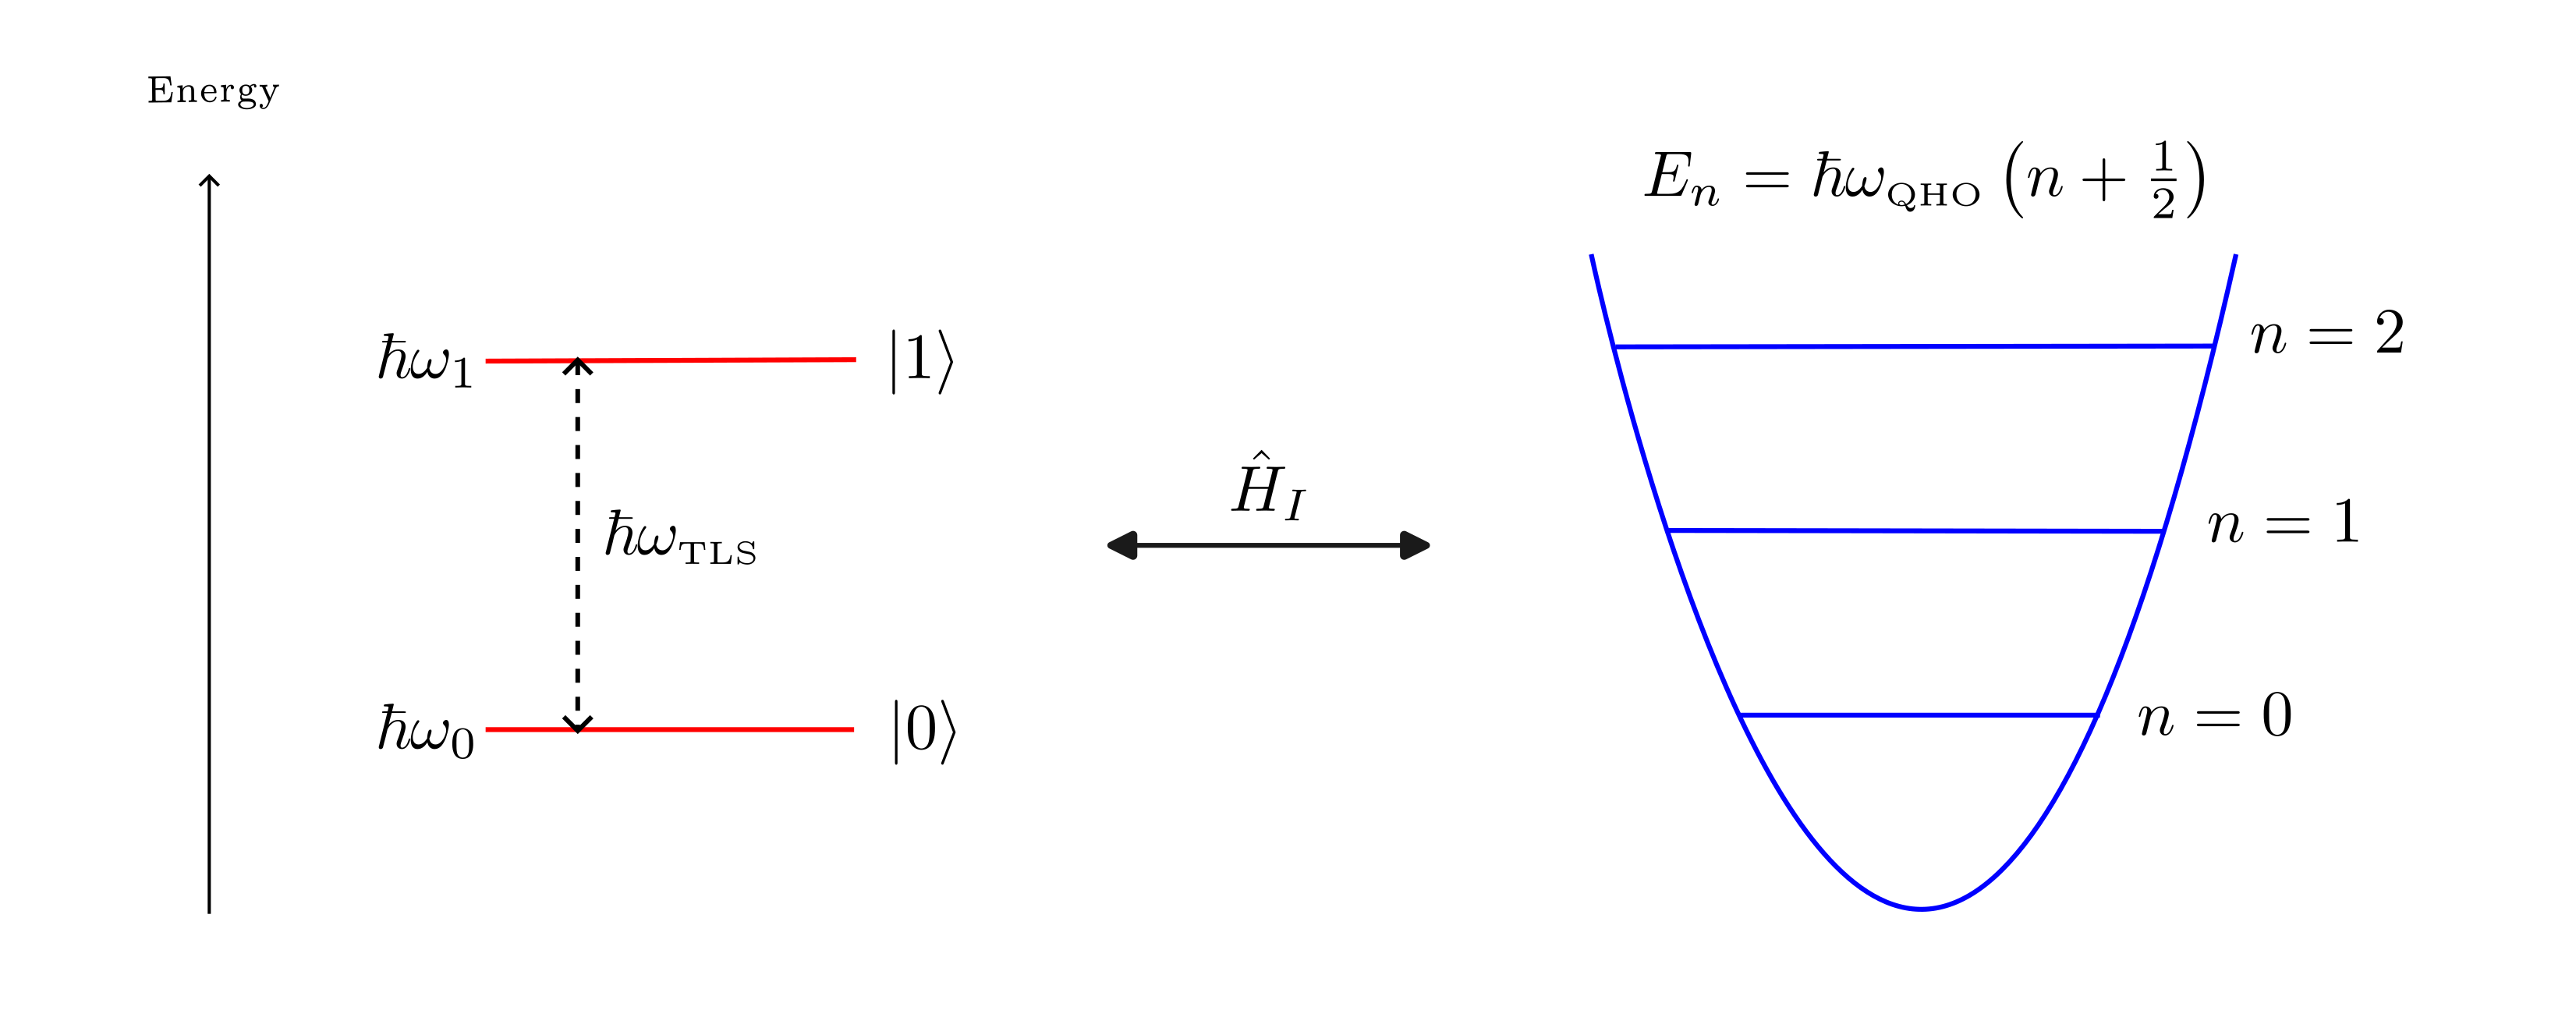
\includegraphics[]{Images/TLSQHO.png}
    \caption{Schematic diagram of a TLS coupled to a QHO. The red lines represent the two distinct energy levels of the TLS, with an energy gap of $\hbar\omega_{\scriptscriptstyle \text{TLS}} = \hbar\left(\omega_1 - \omega_0\right)$. The blue lines represent the quantised energy levels of the QHO, given by $E_n = \hbar\omega_{\scriptscriptstyle \text{QHO}}\left(n+1/2\right)$ with $n=0,1,2\ ...$. $\hat{H}_I$ represents the interaction Hamiltonian, which governs the interaction between the TLS and QHO.}
    \label{img:TLSQHO}
\end{figure}

\noindent In this section, we present the theoretical framework for TLS--QHO systems. This formalism is the basis for a variety of models, including the Jaynes--Cummings and Exciton--Vibration models \cite{Hamiltonian2012-JC_Friction, ExVib2015-ChemPhysBorn}, both of which are central to our later analysis. Developing a clear understanding of how TLS--QHO systems function is essential for exploring how quantum resources manifest in such systems. \\
\\
To understand the entire system, we must first understand each subsystem. We can then examine their interactions as a composite quantum system.

A TLS is a simple yet fundamental quantum mechanical system that can occupy only two distinct energy states. A state vector describing a TLS is written as:

\begin{equation}
    |\psi_{\scriptscriptstyle \text{TLS}}\rangle = \alpha|0\rangle + \beta|1\rangle,
\end{equation}

where $|0\rangle$ and $|1\rangle$ are the basis vectors describing the lower and higher energy states respectively, spanning a 2--dimensional Hilbert Space, $\mathcal{H}_{\scriptscriptstyle \text{TLS}}$ , and $\alpha$ and $\beta$ are the complex amplitudes associated with each basis vector. A TLS can be represented by many quantum systems. Most notably, the simplest form is a qubit, which is often used in quantum computations \cite{TLS2024-qubits}. However, it may also be represented by an atom, with $|0\rangle \rightarrow |g\rangle$ representing the ground (lowest energy) state of an atom, and $|1\rangle \rightarrow |e\rangle$ representing the excited (highest energy) state. Quantum systems may also be reducde to an effective TLS if the system is truncated to only two possible energy states. \\
\\
A QHO is another fundamental quantum mechanical model that describes a system with evenly spaced energy levels, and a quantised energy spectrum. A general state vector describing a QHO is written as:

\begin{equation}
|\psi_{\scriptscriptstyle \text{QHO}}\rangle = \sum_{n=0}^\infty c_n |n\rangle,
\end{equation}

where $|n\rangle$ is the n$^{th}$ Fock state (a state with exactly n quanta of excitation), spanning an infinite--dimensional Hilbert Space $\mathcal{H}_{\scriptscriptstyle \text{QHO}}$, and and $c_n$ are the complex amplitudes associated with each Fock state. A QHO may represent a field confined to a cavity, or molecular vibrations \cite{Context2004-CQED_JCM}.\\
\\
The TLS--QHO composite quantum system is the tensor product of both systems:

\begin{equation}
    |\Psi\rangle = |\psi_{\scriptscriptstyle \text{TLS}}\rangle \otimes |\psi_{\scriptscriptstyle \text{QHO}}\rangle,
\end{equation}

where $|\Psi\rangle$ now resides in the $\mathcal{H}_{\scriptscriptstyle \text{TLS}} \otimes\mathcal{H}_{\scriptscriptstyle \text{QHO}}$ Hilbert space. The Hamiltonian of such a system may be separated into three parts, one for each subsystem (the free Hamiltonians) and one for the interaction of the two systems:

\begin{equation}
    \hat{H} = \hat{H}_{\scriptscriptstyle \text{TLS}} + \hat{H}_{\scriptscriptstyle \text{QHO}} + \hat{H_{\scriptscriptstyle \text{I}}}.
\end{equation}
\\
Such composite systems arise in a wide range of physical contexts and are described by several well-known models. One of these is the quantum Rabi model, introduced in 1936 to model light--matter interactions \cite{Context1936-Rabi}. Furthermore, in 1953, the Dicke model was formulated to describe a large ensemble of atoms (many TLSs) coupled to a single cavity mode \cite{Context1954-Dicke}. However, these models are not analytically solvable because of their complex interaction Hamiltonians. Moreover, they are overly detailed in describing the weak and strong coupling regimes, and are more tailored to the ultrastrong regime and beyond. The Jaynes--Cummings model was originally developed in 1963 to clarify the relationship between quantum radiation and semi--classical theory in the context of cavity QED \cite{Context1963-JC_Original}. In doing so, it also resolved both the suitability and solvability of the Rabi and Dicke models in the weak and strong coupling regimes. Therefore, we shall use the Jaynes--Cummings model to explore quantum resource manifestation in TLS--QHO systems.\\
While it remains a valuable model for study, the Jaynes--Cummings model has been extensively explored and offers limited new insights at this level. Thus, to explore richer dynamics, we must examine more complex models. The exciton--vibration model characterises the interaction between multiple electronic excitations (excitons) and their coupling to quantised vibrational modes. If we consider a dimer containing two excitons and restrict the system to a single excitation, we arrive at a system wherein a single exciton (TLS) is coupled to one vibration (QHO). The model then becomes similar to the Jaynes--Cummings model, albeit with a more complex TLS and interaction description. Thus, this model offers novel dynamics within which we may explore more interesting quantum resource characteristics. \\
\\
Now that we have introduced the TLS–QHO composite system and its Hamiltonian structure, we turn our attention to the theoretical background of our chosen models: the Jaynes–Cummings and the exciton–vibration models. We then examine open quantum dynamics before analysing the effects of entanglement and coherence on quantum systems.

%%%%%%%%%%%%%%%%%%%%%%%%%%%%%%%% JCM %%%%%%%%%%%%%%%%%%%%%%%%%%%%%%%%
\subsubsection{Jaynes--Cummings Model} \label{sec:theory_subsub_JCM}

The Jaynes--Cummings model (JCM) describes a system in which a single TLS is coupled to a single quantised mode of the QHO. The model has found wide application, as outlined in our literature review. One prominent realisation is cavity QED, as shown in Figure \ref{fig:img_JCM}, where an atom interacts with a quantised cavity field. In this setting, a 2024 study presented a method for achieving a deep-strong coupling regime for a JCM system by modulating the transition frequency of the TLS \cite{Context2024-CQED_JCM}. In the same year, the non-linear JCM, an extension of the JCM, was employed to investigate the effects of non--linearity in superconducting quantum circuits \cite{Context2024-CircuitQED}. The JCM has also been applied in the study of nitrogen-vacancy centres, where interference phenomena in diamond nanocrystals have been explored \cite{Context2009-Alt_NVcentres}. 
\begin{figure}[h]
    \centering
    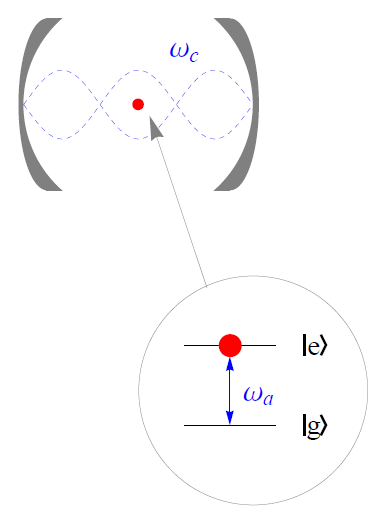
\includegraphics[scale=0.5]{Images/Jaynes-Cummings_model.png}
    \caption{Example of the JCM in the context of cavity QED. The atom, modelled as a TLS with frequency $\omega_a$, is the red dot on the top left. The atom resides in an optical cavity, modelled as a QHO with frequency $\omega_c$. Image adapted from \cite{Image-Prince_JCM}. Used under the terms of the CC BY-SA 3.0 license.}
    \label{fig:img_JCM}
\end{figure}

\noindent The Hamiltonian describing the JCM may be written as:

\begin{equation} \label{JC_H}
    \hat{H}_{\scriptscriptstyle \text{JC}} = \frac{\hbar\omega_a}{2}\hat{\sigma}_z + \hbar\omega_c\left(\hat{a}^\dagger \hat{a} + \frac{1}{2} \right) + g(\hat{a}\hat{\sigma}_{+} + \hat{a}^\dagger\hat{\sigma}_{-}), 
\end{equation} 
with 
\begin{align*}
    \begin{aligned}
        \hat{H}_{\scriptscriptstyle \text{TLS}} &\equiv \frac{\hbar\omega_a}{2}\hat{\sigma}_z \\
        \hat{H}_{\scriptscriptstyle \text{QHO}} &\equiv \hbar\omega_c\left(\hat{a}^\dagger \hat{a} + \frac{1}{2} \right) \\
        \hat{H}_{\scriptscriptstyle \text{I}} &\equiv \hbar g(\hat{\sigma}_{+}\hat{a} +\hat{\sigma}_{-}\hat{a}^\dagger).
    \end{aligned}
\end{align*}

In Equation \eqref{JC_H}, $\omega_a$ is the excitation frequency of the TLS, $\omega_c$ is excitation frequency of the QHO, and $g$ is the coupling strength constant. $\hat{\sigma}_z, \hat{\sigma}_+, \text{and } \hat{\sigma}_-$ are Pauli spin operators of the form $\hat{\sigma}_z = |1\rangle\langle1| - |0\rangle\langle0|, \hat{\sigma}_+ = |1\rangle\langle0|, \text{and } \hat{\sigma}_- = |0\rangle\langle1|$ which act upon the TLS. The operators $\hat{a}, \hat{a}^\dagger$ act solely on the QHO, such that $\hat{a}|n\rangle = \sqrt{n}|n-1\rangle$ acts to lower the state of the QHO, and $\hat{a}^{\dagger}|n\rangle = \sqrt{n+1}|n+1\rangle$ acts to raise the state of the QHO.\\
\\
The JCM is a simple model that is exactly solvable. Its simplicity arises from a set of four key approximations that constrain the model’s applicability to specific systems and coupling regimes \cite{General2024-JC_overview}. 

The first approximation is the dipole approximation. Here, we consider the QHO to be uniform, such that the interaction Hamiltonian of the JCM can be modelled by a dipole (with energy $\boldsymbol{\hat{d}}$) in a uniform electric field $\boldsymbol{\hat{E}}$, such that:

\begin{equation*}
    \hat{H}_{\scriptscriptstyle \text{I}} \propto \boldsymbol{\hat{d}} \cdot \boldsymbol{\hat{E}}.
\end{equation*}

The second approximation is the single mode approximation. Here, we take the infinite set of quantised modes of the field and discard all except the mode whose frequency is closest to the transition frequency of the TLS (the resonant mode where $\omega_a = \omega_c$). Thus, the dynamics can be described as a QHO \cite{General2024-JCM_relevance}. In the dipole approximation, the electric field becomes

\begin{equation*}
    \boldsymbol{\hat{E}}  \propto \hat{a} + \hat{a}^\dagger.
\end{equation*}


The third approximation is the TLS approximation. Many quantum systems, such as atoms have numerous discrete energy levels. The JCM, however, only considers the two lowest energy levels of the system, $|0\rangle$ and $|1\rangle$, and all higher energy levels are neglected. The approximation is only valid when the system is weakly driven, such that the higher energy levels are negligible, and the system may be described as a TLS. In the dipole approximation, the dipole energy becomes:

\begin{equation*}
    \boldsymbol{\hat{d}}  \propto \hat{\sigma}_{-} + \hat{\sigma}_{+}.
\end{equation*}

The last approximation is the Rotating Wave Approximation (RWA). In the full interaction Hamiltonian, the product of the electric field and dipole operator under the RWA becomes

\begin{equation}
    \boldsymbol{\hat{d}} \cdot \boldsymbol{\hat{E}} \propto (\hat{\sigma}_{-} + \hat{\sigma}_{+})(\hat{a} + \hat{a}^\dagger) \approx \hat{\sigma}_{+}\hat{a} +\hat{\sigma}_{-}\hat{a}^\dagger. 
\end{equation}

The RWA neglects the terms $\hat{\sigma}_{-}\hat{a}, \hat{\sigma}_{+}\hat{a}^\dagger$ of the quadratic expansion, which oscillate rapidly. However, this approximation is only valid when the coupling strength of the interaction $g$ is much less than the characteristic frequencies $\omega_a$ and $\omega_c$. \\
\\
These approximations, particularly the RWA, restrict the JCM to certain physical regimes. Indeed, the JCM primarily concerns itself with systems in the strong--coupling regime \cite{General2024-JCM_relevance}. We now introduce three key conditions for upholding this physical regime.
\begin{equation} \label{JCM_condition_g<omega}
    g \ll \omega_a, \omega_c 
\end{equation} 

must be held to ensure that the RWA remains valid. Furthermore, we introduce the cooperativity parameter:

\begin{equation} \label{JCM_condition_cooperativity}
    C = \frac{4g^2}{\gamma\cdot\gamma_{\scriptscriptstyle th}} > 1
\end{equation}

where $\gamma, \gamma_{\scriptscriptstyle th}$ are the decay rates owing to spontaneous atomic emission and thermal decay respectively. Finally, we introduce the normalised coupling parameter, 

\begin{equation} \label{JCM_condition_norm_coupling}
    \zeta = \frac{4g^2}{\omega_a\cdot\omega_c} < 0.04
\end{equation}, 

with $\zeta \approx \mathcal{O}(1)$ indicating an ultrastrong--coupling regime in which the condition in equation \eqref{JCM_condition_g<omega} is no longer held, and the discarded terms under the RWA approximation are no longer negligible.\\
\\
If we remain in valid coupling regimes, the JCM is a strong model for studying quantum resources in TLS--QHO systems. In fact, certain characteristic features are captured by the JCM which are key to understanding the nature of the light--matter interactions it describes. 

One key characteristic of the JCM is Rabi oscillations, which are coherent, periodic exchanges of excitation between the TLS and QHO. The interaction Hamiltonian in Equation \eqref{JC_H} creates a flip--flop effect, where an excitation in the TLS causes a photon to be destroyed in the QHO and de--excitation causes a photon to be created. The interaction Hamiltonian clearly shows this periodic exchange of energy via the coupling of the annihilation operator $\hat{a}$ with the atomic excitation operator $\hat{\sigma}_+$, and $\hat{a}^\dagger$ with $\hat{\sigma}_-$.

This operator coupling further leads to the conservation of the excitation number operator $\hat{N} = \hat{a}^\dagger \hat{a} + \frac{1}{2}(1 + \hat{\sigma}_z)$. The excitation number operator commutes with the Hamiltonian ($[\hat{N}, \hat{H}_{\scriptscriptstyle \text{JC}}] = 0$); therefore $\hat{N}$ is conserved. As a consequence, the JCM only allows transitions between states with the same excitation number, such as $|g, n+1\rangle$ and $|e,n\rangle$. For example, states such as

\begin{equation} \label{JCM_general_state}
    |\psi\rangle = \alpha|g,n+1\rangle + \beta|e,n\rangle
\end{equation} 

are allowed, and such states will be explored in Section \ref{sec:results_JCM}.\\
\\
It is clear that the JCM's simplicity, arising from the aforementioned approximations, allows it to capture interesting phenomena such as Rabi oscillations. However, owing to its popularity and age, quantum resources in the JCM have been studied extensively, and are well documented. To explore more novel manifestations of these quantum resources, we turn to the exciton--vibration model. 

%%%%%%%%%%%%%%%%%%%%%%%%%%%%%%%% EVM %%%%%%%%%%%%%%%%%%%%%%%%%%%%%%%%
\subsubsection{Exciton--Vibration Model}  \label{sec:theory_subsub_EVM}
The exciton--vibration model (EVM) describes the interaction between multiple electronic excitations (excitons) and quantised vibrational modes. For a general EVM, the excitons are modelled by TLSs, and the QHO is modelled by the quantised vibrational modes that are local to each site. One of the first explicit formulations of the EVM can be found in the 1996 paper by Schanz et al., in which two excitons are modelled by a dimer, which are in turn coupled to local vibrational modes \cite{ExVib1997-First}. The EVM has since been deployed in the field of chemical physics to study entanglement and the breakdown of the Born--Oppenheimer approximation, which treats nuclear and electronic dynamics separately \cite{ExVib2015-ChemPhysBorn}. Moreover, in quantum biology, the exciton is modelled by a dimer to investigate enhanced exciton--vibration energy exchange in light harvesting complexes at room temperature \cite{ExVib2014-Alexandra}.\\

\begin{figure}[H]
    \centering
    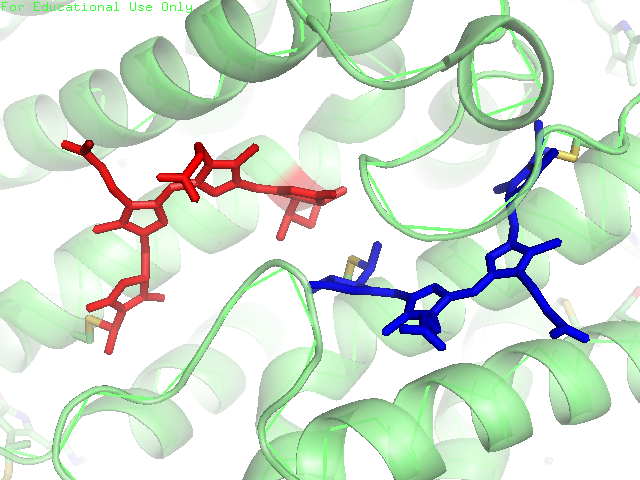
\includegraphics[width=0.5\linewidth]{Images/PEB50dimer.png}
    \caption{Schematic diagram of the central dimer of the protein phycoerythrin 545 (PE545) drawn based on PDB 1XG0. The two pigments forming the dimer are shown in red and blue, representing chromophores that host excitons. The green helices depict the surrounding protein. Courtesy of Prof. Olaya--Castro.}
    \label{fig:dimer}
\end{figure}

\noindent We consider a special case of the EVM which is consistent with reference \cite{ExVib2014-Alexandra} in which a dimer is coupled to local vibrational modes. A dimer contains two chromophores (sites), each of which contains an exciton, as illustrated in Figure \ref{fig:dimer}. Consequently, each exciton is coupled to a local vibrational mode called a phonon. The Hamiltonian of this model is expressed as

\begin{equation} \label{eqn:H_EV_general}
    \hat{H}_{\scriptscriptstyle \text{EV}} = \sum_{i=1,2}\epsilon_i\hat{\sigma}_{+,i}\hat{\sigma}_{-,i} + V\left(\hat{\sigma}_{+,1}\hat{\sigma}_{-,2}+\hat{\sigma}_{+,2}\hat{\sigma}_{-,1}\right)
    + \omega_{\scriptscriptstyle \text{vib}} \left(\hat{b}_1^\dagger \hat{b}_1 + \hat{b}_2^\dagger \hat{b}_2\right)
    + g\sum_{i=1,2}\hat{\sigma}_{+,i}\hat{\sigma}_{-,i}\left(\hat{b}_i^\dagger + \hat{b}_i\right),
\end{equation}

with 

\begin{align*}
    \begin{aligned}
        \hat{H}_{\scriptscriptstyle \text{TLS}} &\equiv \sum_{i=1,2}\epsilon_i\hat{\sigma}_{+,i}\hat{\sigma}_{-,i} + V\left(\hat{\sigma}_{+,1}\hat{\sigma}_{-,2}+\hat{\sigma}_{+,2}\hat{\sigma}_{-,1}\right) \\
        \hat{H}_{\scriptscriptstyle \text{QHO}} &\equiv \omega_{\scriptscriptstyle \text{vib}} \left(\hat{b}_1^\dagger \hat{b}_1 + \hat{b}_2^\dagger \hat{b}_2\right) \\
        \hat{H}_{\scriptscriptstyle \text{I}} &\equiv g\sum_{i=1,2}\hat{\sigma}_{+,i}\hat{\sigma}_{-,i}\left(\hat{b}_i^\dagger + \hat{b}_i\right)
    \end{aligned}
\end{align*}

In equation \eqref{eqn:H_EV_general}, $\epsilon_i$ is site $i$'s excited state energy, $V$ is the coupling strength between the two sites, $\omega_{\scriptscriptstyle \text{vib}}$ is the frequency of the vibrational mode, and $g$ is the coupling strength of the excitons and vibrational modes. The Pauli operators $\hat{\sigma}_{\pm,i}$ act to raise/lower the excitation of a site $i$, whereas the operators $\hat{b}_i, \hat{b}_i^\dagger$ annihilate/create a phonon of the vibrational mode of a site $i$.\\
\\
\noindent To introduce the simplified Hamiltonian which will be the focus of our study, we first outline two key procedures.\\
\\
We first restrict the dimer to a single excitation, leaving only states with an excitation localised on one site, allowing us to model the dimer (and thus its two chromophores) as a single effective TLS.

Second, we transform the two local vibrational modes into collective coordinates. We observe that the centre of mass mode $\hat{b}_{\scriptscriptstyle \text{cm}}$ decouples from the exciton dynamics; therefore, only the relative displacement mode $\hat{b}_{\scriptscriptstyle \text{rd}}$ couples to the exciton. Thus, we reduce the two QHOs to one.

These two procedures are schematically illustrated in Figure \ref{fig:img_EVM}, which shows how the general dimer model with two local vibrational modes reduces to an effective single TLS coupled to a single collective vibrational mode.\\
\\
Our Hamiltonian in equation \eqref{eqn:H_EV_general} then reduces to the following:

\begin{equation} \label{eqn:H_EV}
    \hat{H}_{\scriptscriptstyle \text{EV}} = \frac{\Delta\epsilon}{2}\hat{\sigma}_z + V\hat{\sigma}_x + \omega_{\scriptscriptstyle \text{vib}} \hat{b}_{\scriptscriptstyle \text{rd}}^\dagger \hat{b}_{\scriptscriptstyle \text{rd}} -\frac{g}{\sqrt{2}}\hat{\sigma}_z\left(\hat{b}_{\scriptscriptstyle \text{rd}}^\dagger + \hat{b}_{\scriptscriptstyle \text{rd}}\right),
\end{equation}

with 
\begin{align*}
    \begin{aligned}
        \hat{H}_{\scriptscriptstyle \text{TLS}} &\equiv \frac{\Delta\epsilon}{2}\hat{\sigma}_z + V\hat{\sigma}_x \\
        \hat{H}_{\scriptscriptstyle \text{QHO}} &\equiv \omega_{\scriptscriptstyle \text{vib}} \hat{b}_{\scriptscriptstyle \text{rd}}^\dagger \hat{b}_{\scriptscriptstyle \text{rd}} \\
        \hat{H}_{\scriptscriptstyle \text{I}} &\equiv-\frac{g}{\sqrt{2}}\hat{\sigma}_z\left(\hat{b}_{\scriptscriptstyle \text{rd}}^\dagger + \hat{b}_{\scriptscriptstyle \text{rd}}\right),
    \end{aligned}
\end{align*}

where $\Delta\epsilon = \epsilon_1 - \epsilon_2$ is the site energy difference between the two chromophores. \\

\begin{figure}[h]
    \centering
    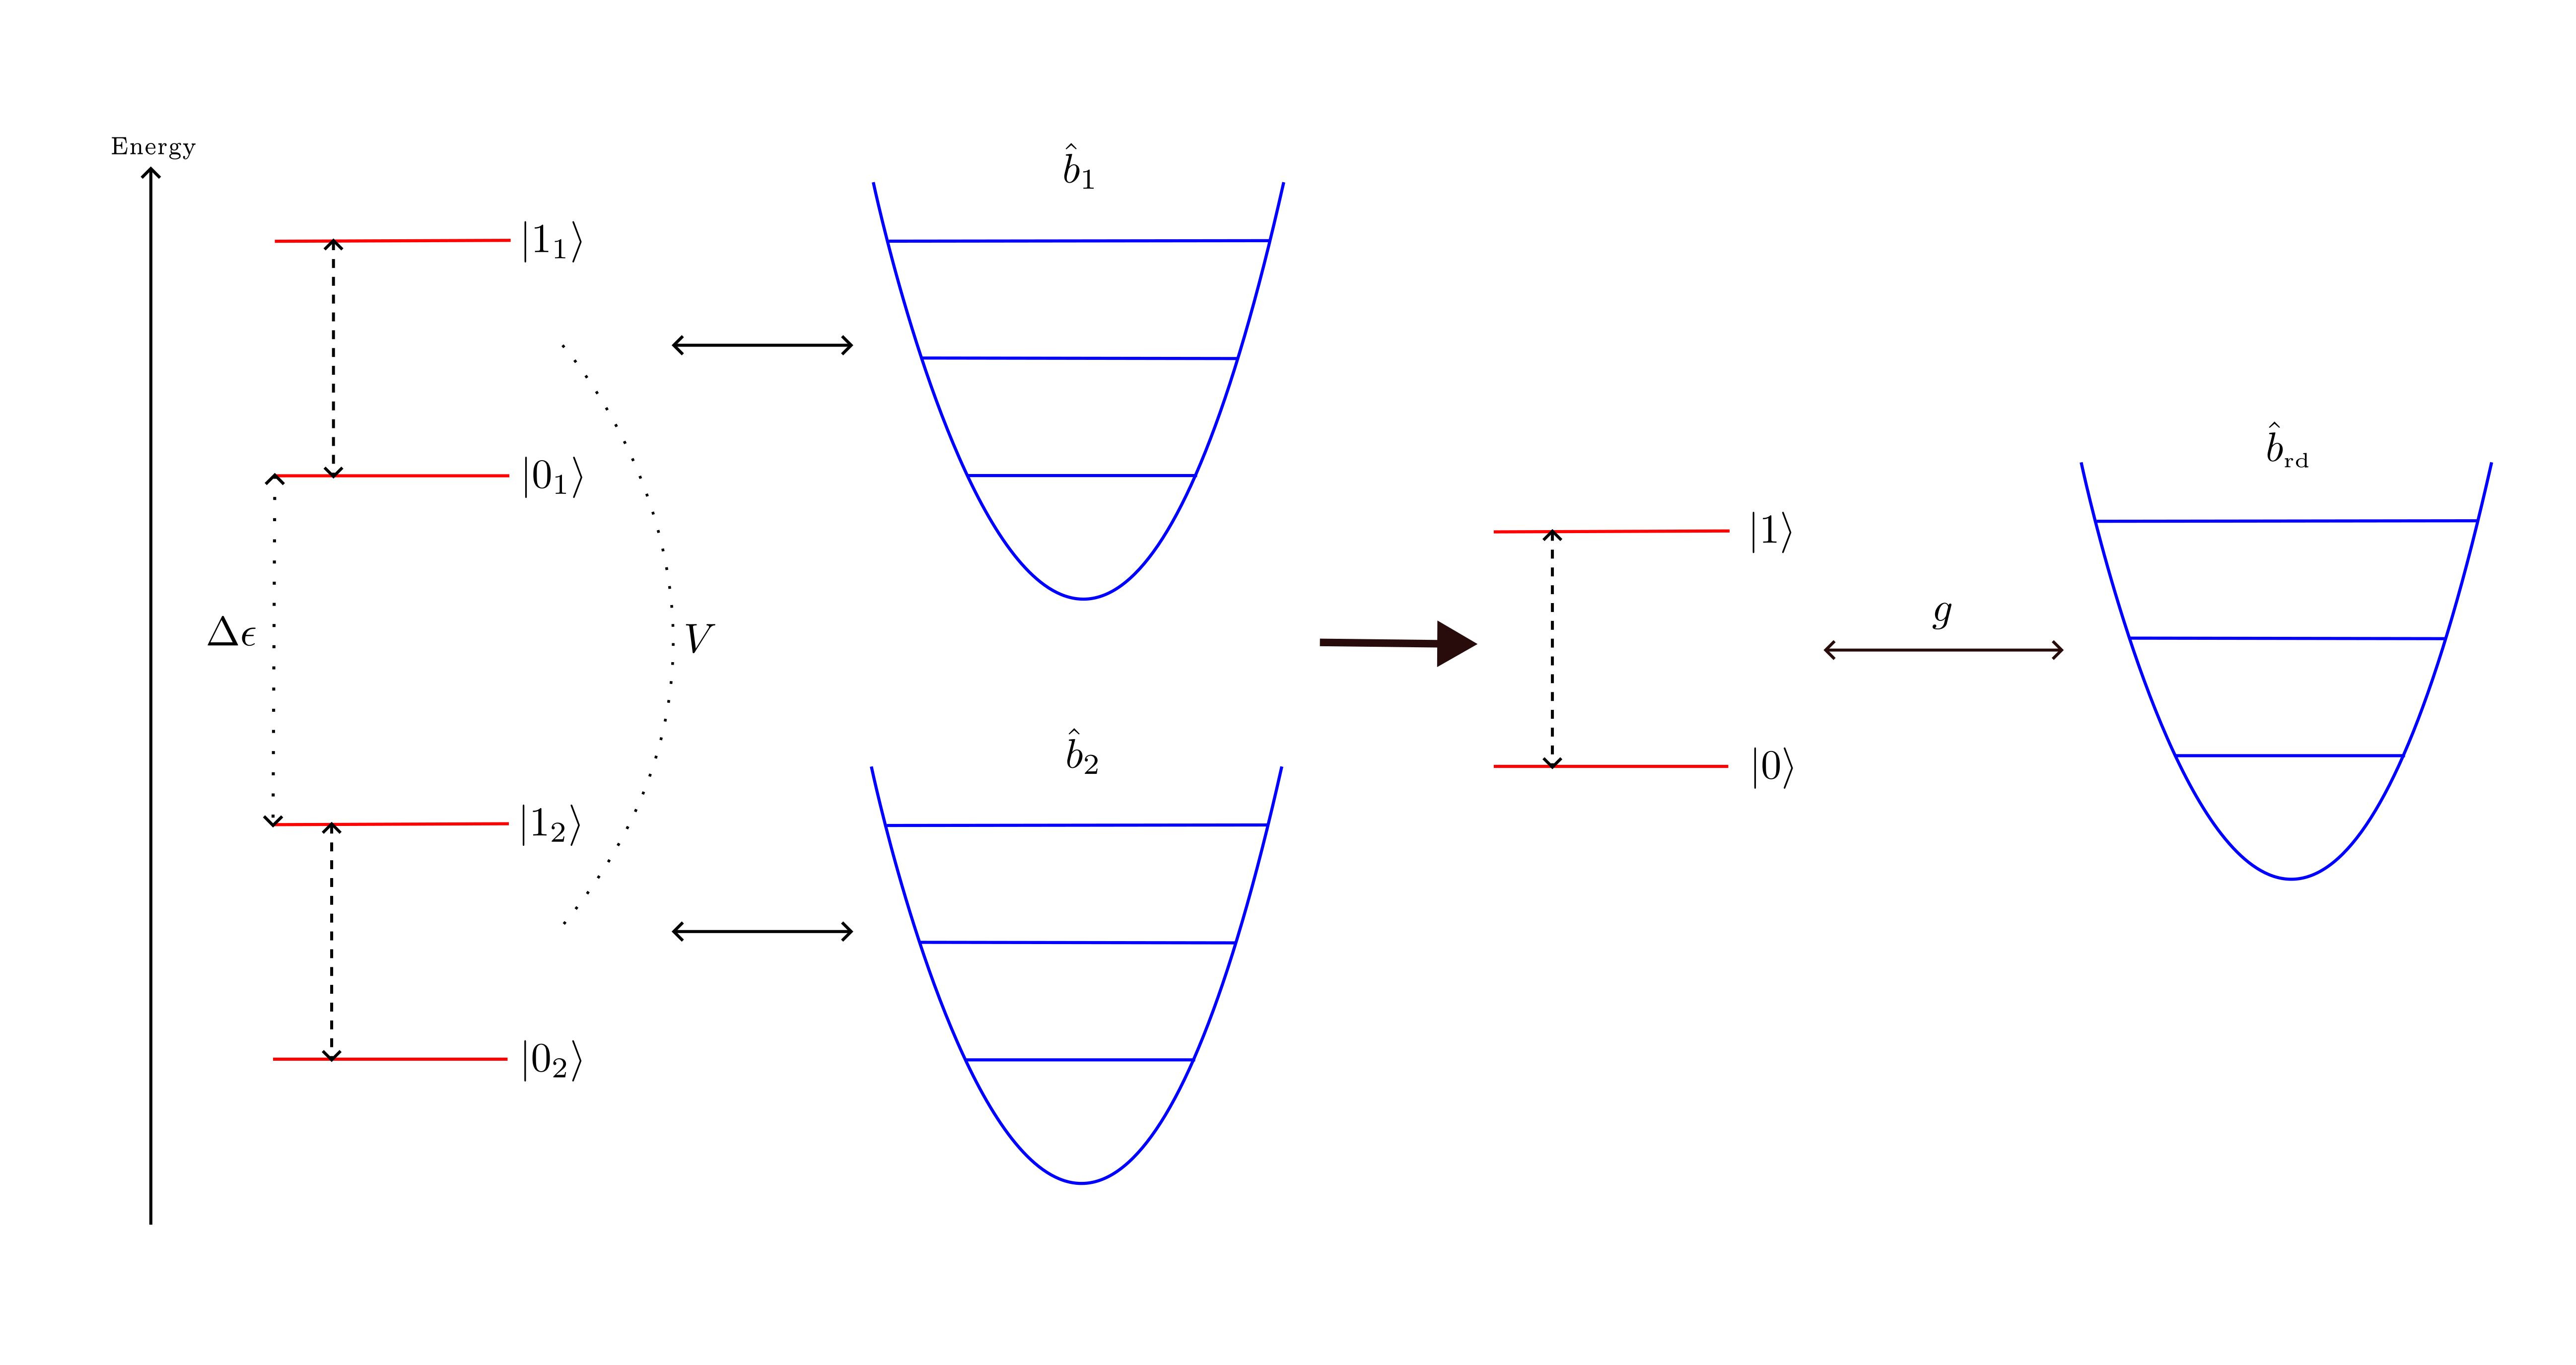
\includegraphics[scale=0.7]{Images/EVM.png}
    \caption{Schematic diagram of the EVM. The left--hand side shows two excitons (which represent the two chromophores in a dimer), with an inter--exciton coupling strength $V$ and an energy gap $\Delta\epsilon$. The QHO with $\hat{b}_1$ is coupled to the first chromophore (site 1), and the QHO with $\hat{b}_2$ is coupled to the second chromophore (site 2). The right--pointing thick arrow in the centre of the diagram represents the single excitation restriction and collective coordinate transformation. The right--hand side shows the effective single--TLS exciton, coupled to the collective vibration $\hat{b}_{\scriptscriptstyle \text{rd}}$ with a coupling strength $g$.}
    \label{fig:img_EVM}
\end{figure}

\noindent This Hamiltonian is similar to the Jaynes–-Cummings Hamiltonian in equation \eqref{JC_H}, but differs by including an additional TLS and interaction term, making the EVM a slightly more complex variant that enables the study of richer dynamics. Furthermore, although this model shares some characteristics with the JCM, it differs in other, more interesting ways. \\
\\
The EVM exhibits coherent energy exchange when the excitonic energy--splitting resonates with the vibrational mode frequency. This resonant coupling sustains oscillations akin to the JCM's Rabi oscillations between the two subsystems, even under incoherent excitation. Moreover, the additional TLS term $V\hat{\sigma}_x$ introduces a direct coupling between the two excitonic states, providing an extra channel for the generation of non--classical correlations such as entanglement and coherence. Thus, while population transfer for the exciton only occurs through the $V\hat{\sigma}_x$, the vibration subsystem transfers its populations through the interaction Hamiltonian.\\
\\
Now that we have a more complete understanding of the JCM and EVM, we need to explore how these models evolve. To do so, we must examine both the idealised closed evolution, and the more physically relevant open evolution of the system. Therefore, we turn to the general framework of open quantum systems, which forms the basis for analysing the time evolution of both models.

%%%%%%%%%%%%%%%%%%%%%%%%%%%%%%%% OQS %%%%%%%%%%%%%%%%%%%%%%%%%%%%%%%%
\subsection{Open Quantum Systems} \label{sec:theory_sub_OQS}

In quantum theory, the evolution of a system can be treated in two distinct ways: a closed system approach, where the system is isolated from its environment, and an open system approach, where the external environment directly influences the dynamics. While closed system evolution is sufficient for examining a snapshot of the behaviour of a model, the open evolution ultimately determines how the system behaves in physical settings. We now proceed to define the theoretical mechanisms of closed system evolution before doing the same for open system evolution.\\
\\
For an initial state $|\psi (t=0)\rangle$, its closed evolution is governed by

\begin{equation} \label{eqn:closed_evo}
    |\psi(t)\rangle = \hat{U}(t)|\psi(t=0)\rangle,
\end{equation}

where the unitary evolution operator $\hat{U}(t) = e^{i\hat{H}t/\hbar}$ is defined for a time-independent Hamiltonian $\hat{H}$. The exponentiation of the Hamiltonian operator is significantly simplified if the Hamiltonian is diagonal. For example, consider the diagonal Hamiltonian $\hat{H}$:

\begin{equation*}
    \hat{H} = 
    \begin{bmatrix}
        \lambda_1 & 0 \\
        0 & \lambda_2
    \end{bmatrix},
\end{equation*}, 

which is exponentiated as

\begin{equation*}
    e^{\hat{H}} = \sum_j 
    \begin{bmatrix}
        \lambda_i^j/j! & 0 \\
        0 & \lambda_2^j/j!
    \end{bmatrix}
    = \begin{bmatrix}
        e^{\lambda_1} & 0 \\
        0 & e^{\lambda_2}
    \end{bmatrix}.
\end{equation*}

\noindent Understanding how a closed system evolves provides insights into the key characteristics of a system. For example, closed evolution may illuminate population and coherence oscillations of exciton--vibration systems such as dimers in light--harvesting biological complexes \cite{ExVib2014-Alexandra}. We can also observe how Rabi oscillations of the JCM lead to oscillations in entanglement and coherence \cite{Entanglement2009-REE_VNapplied}. However, to capture the complete physics of TLS--QHO systems, their evolution must be examined under open quantum dynamics. In fact, many studies, including the aforementioned ones, take the approach to begin by looking at closed system evolution, and then proceed to look at open system evolution when the core dynamics of the system are understood.\\

\begin{figure}[h]
    \centering
    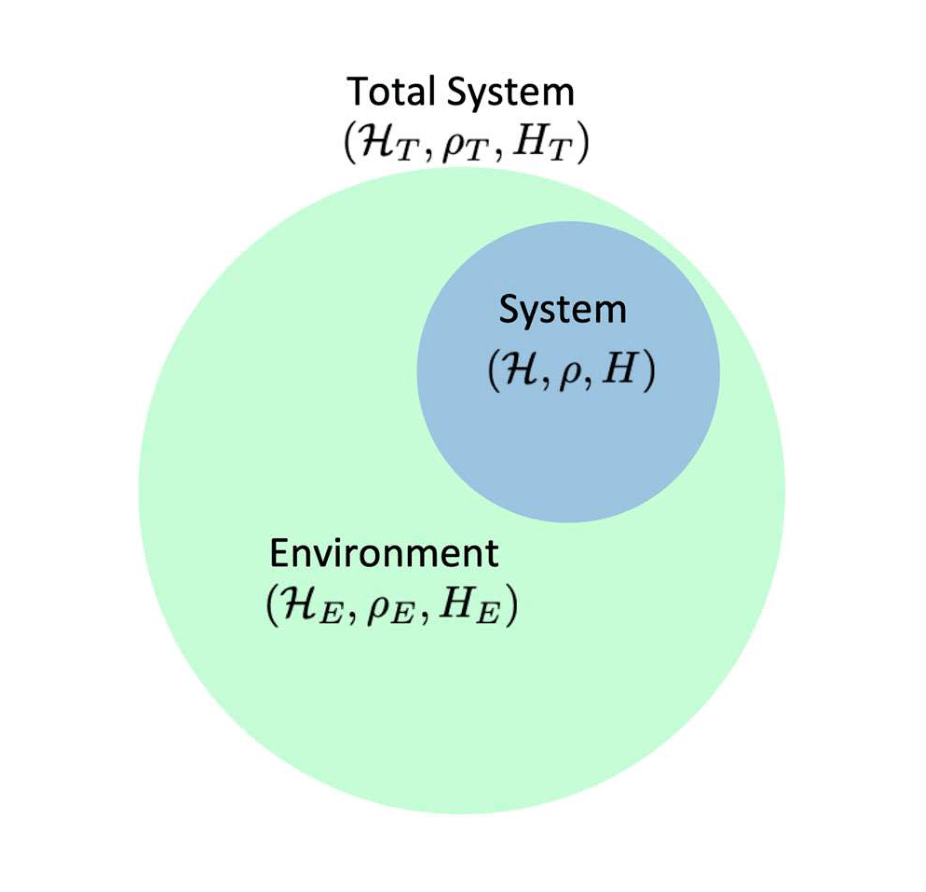
\includegraphics[scale=0.55]{Images/open_q_sys.png}
    \caption{Open quantum systems schematic diagram. The system is represented by the state $\rho$ with a Hamiltonian $H$ governing its dynamics, and resides in the Hilbert space $\mathcal{H}$. It is surrounded by an environment, represented by the state $\rho_{\scriptscriptstyle \text{E}}$ with a Hamiltonian $H_{\scriptscriptstyle \text{E}}$ and resides in the Hilbert space $\mathcal{H}_{\scriptscriptstyle \text{E}}$. Under open quantum systems, we take into account both the system and its environment, such that the total system is represented by the state $\rho_{\scriptscriptstyle \text{T}}$ with a joint Hamiltonian $H_{\scriptscriptstyle \text{T}}$ and a joint Hilbert space $\mathcal{H}_{\scriptscriptstyle \text{T}}$. Image adapted from \cite{Image2020-OQS}. Used under the terms of the CC BY-SA 4.0
        license.}
    \label{fig:img_OQS}
\end{figure}\\

\noindent An open quantum system is any system that takes into account its environment, such that there is a minimum transfer of information between the environment and the system. This is schematically illustrated in Figure \ref{fig:img_OQS}, where the system interacts with its surrounding environment to form a composite system. There are two types of open system evolution: Markovian and non-Markovian.

Markovian evolution describes dynamics in which the system's future evolution depends only on its current state and not on its history; as such, the environment has no memory. 

In contrast, non-Markovian evolution occurs when the environment retains memory of its interaction with the system, allowing information to flow back into the system. Future states depend on both the current state of the system and its history. 

In this work, we adopt the Markovian approach to open-system evolution for its relative simplicity, as our primary goal is to illustrate how entanglement and coherence evolve. To evolve our state in this manner, we need to define a master equation, that tells us how the state of a system changes over time when using a density matrix as a state descriptor. The Lindblad equation is a general form of a Markovian master equation, and is written as 

\begin{equation} \label{eqn:lindblad}
    \dot \rho(t) = - i[\hat{H}, \rho(t)] + \sum_i\left(L_i\rho(t)L_i^\dagger - \frac{1}{2}\{L_i^\dagger L_i,\rho(t)\} \right) \equiv \mathcal{L}\rho(t).
\end{equation} 

In equation \ref{eqn:lindblad}, $[L_i^\dagger L_i, \rho (t)] = L_i^\dagger L_i\rho(t) + \rho(t)L_i^\dagger L_i$ is an anti--commutator. $L$ are the Lindblad operators, that define how the environments couple to the system and hence how the system decays; they correspond to different types of decay channels. $\mathcal{L}$ is the Liouvillian superoperator (a mathematical object which acts on operators). Solving the Lindblad equation requires handling a set of first--order differential equations, which yields the full time evolution of the system. \\
\\
This particular form of the Lindblad equation is particularly notable, because it separates the unitary, closed evolution part of the system from the open, decay elements. If, for instance, we set all the Lindblad decay operators to 0, we are left with:

\begin{equation}
    \dot \rho(t) = - i[\hat{H}, \rho(t)],
\end{equation}

which is the von Neumann equation. In this formulation, the environment is completely ignored and our system evolves under closed dynamics. As mentioned, the decay operators $L$ represent the different types of channels through which the system decays. Many decay operators can be used in TLS--QHO systems. We selected two specific decay channels for our analysis: spontaneous atomic emission and thermal dissipation. 

Spontaneous atomic emission models the excitation decay in the TLS, representing one of the most fundamental and unavoidable losses in TLS--QHO systems. In terms of the decay operator, spontaneous atomic emission is modelled as

\begin{equation} \label{eqn:L_spont}
    L = \gamma|0\rangle\langle1|,
\end{equation}

where $\gamma$ is the rate of decay, and $|0\rangle,|1\rangle$ represent the ground and excited states respectively. The strength of this decay model is its simplicity, as it captures the essential physics of excitation loss with a single parameter while remaining straightforward to implement in the Lindblad formalism.

Another decay channel that we consider is thermal dissipation. This decay models the energy loss of the QHO to a finite--temperature environment, thus capturing the effect of thermal photons/phonons that drive the oscillator towards equilibrium with its surroundings. The thermal dissipation decay operators are written as follows:

\begin{equation}\label{eqn:L_therm}
    L_1 = \gamma_{\scriptscriptstyle \text{th}}(N+1)\hat{a} 
\end{equation}

and 

\begin{equation*}
    L_2 = \gamma_{\scriptscriptstyle \text{th}}N\hat{a}^\dagger ,
\end{equation*}

where $\gamma_{\scriptscriptstyle \text{th}}$ is the thermal rate of decay, and $\hat{a},\hat{a}^\dagger$ act to annihilate/create a photon (phonon) in the QHO. 
The mean thermal occupation number is defined as 
\begin{equation} \label{therm_occ_num}
    N = [\text{exp}(\omega/k_bT) -1]^{-1},
\end{equation}
where $T$ is the temperature of the bath to which system is coupled, $\omega$ is the frequency of the QHO, and $k_b$ is the Boltzmann constant. These decay operators not only govern energy loss in the TLS and QHO, but also play a central role in driving decoherence.\\
\\
Decoherence refers to the decay of off--diagonal elements of a density matrix in a given basis, indicating a loss of quantum superposition. Decoherence is induced by environmental interactions which are captured by the decay operators $L$. Since the magnitude of these off–diagonal elements directly quantifies coherence, decoherence corresponds to the gradual reduction of this quantum resource, ultimately driving the system towards classical behaviour. In the next section, we explicitly define coherence and its quantifiers. \\
\\
While decoherence describes how quantum resources diminish over time, efficiently simulating such processes requires a suitable mathematical framework. One powerful approach is vectorisation, which is a method used to transform operators into vectors and superoperators into operators. Noting that matrices form a vector space, we define a Hilbert space of matrices, called the Fock--Liouville space (FLS). In this space, an operator such as $|i\rangle\langle j| \rightarrow |j\rangle \otimes |i\rangle$. For a density matrix, $\rho$, 

\begin{equation*}
    \rho = \sum_{i,j}\rho_{i,j}|i\rangle\langle j| \rightarrow \sum_{i,j}\rho_{i,j}|i\rangle\otimes |j\rangle
\end{equation*}

In matrix--vector column notation, this translates to 

\begin{equation*}
    \text{vec}\begin{bmatrix}
        a & b \\
        c & d
    \end{bmatrix}
    = \begin{bmatrix}
        a\\
        b\\
        c\\
        d
    \end{bmatrix}.
\end{equation*}

In terms of bra--ket notation, $\text{vec}(\rho) = |\rho \rangle\rangle.$ Thus, we see that the rank of an operator is reduced by 1, and thus any vectorised operator behaves as a vector in the FLS. Moreover, we observe that for superoperators, their rank also reduces by 1 and thus they behave like operators instead. A key property of the FLS is

\begin{equation*}
    \text{vec}(ABC) = (C^T \otimes A)\text{vec}(B),
\end{equation*}

where $A,B,C$ are operators or superoperators. If we apply vectorisation to the Lindblad master equation, we obtain the following:

\begin{equation}
    \frac{d}{dt}|\rho\rangle\rangle = \hat{\mathcal{L}}|\rho\rangle\rangle,
\end{equation}

where the Liouvillian matrix $\hat{\mathcal{L}}$ is written as:

\begin{equation}
    \hat{\mathcal{L}} = -i\left( \mathds{1} \otimes \hat{H} - \hat{H}^T \otimes \mathds{1}  \right) + \sum_k \gamma_k\left(L_k^*\otimes L_k - \frac{1}{2}\left(\mathds{1} \otimes L_k^\dagger L_k + (L_k^\dagger L_k)^T\otimes \mathds{1} \right) \right),
\end{equation}

where $\gamma_k$ is the decay rate associated with the $k^{th}$ decay operator $L_k$.This form of the Lindblad equation makes it especially useful for computational methods, as it transforms the set of linear differential equations into a matrix--vector problem. In libraries such as Python's QuTip, master equation solvers use this method to evolve input states \cite{Comp2012-Qutip}.\\
\\
Having established the framework for modelling TLS--QHO systems under both closed and open evolution, and the role of environmental interactions through the Lindblad formalism, we now turn to the specific quantum resources of interest in this work. In particular, we focus on entanglement and coherence, as they capture the essential non-classical features whose dynamics we aim to investigate.
%%%%%%%%%%%%%%%%%%%%%%%%%%%%%%% Q RESOURCES %%%%%%%%%%%%%%%%%%%%%%%%%%%%%%%%%%%%%%%%%%
\subsection{Quantum Resources} \label{sec:theory_sub_ent}

Quantum resources are fundamental properties of quantum systems that enable us to perform computations and improve a system's efficiency and are essential for leveraging the unique advantages of quantum mechanics over classical physics. Two of the most essential resources we study are entanglement and coherence. To inspect how these resources manifest in TLS--QHO systems, we must understand and quantify them. This section focuses on the explanation and quantification of entanglement and coherence and how they might be used to learn more about our system in question. 

\subsubsection{Entanglement}

One of the most celebrated quantum resources is entanglement, a unique quantum phenomenon that describes non--classical correlations between subsystems of a composite quantum system. A total state $|\Psi\rangle$ is said to be entangled if it cannot be written as a product state; that is

\begin{equation}
    |\Psi\rangle \neq |\psi_A\rangle \otimes |\psi_B\rangle,
\end{equation}

where $|\psi_A\rangle, |\psi_B\rangle$ are the pure states of subsystems A and B, respectively, and $|\Psi\rangle$ is entangled \cite{Entanglement1999-Overview_&REE}. If a state \textit{can} be written as a product state, it is considered separable and exhibits only classical correlations. However, entangled states exhibit non--local correlations that can violate Bell Inequalities, which can be demonstrated using, for example, the GHZ game. 

In physical systems such as the TLS--QHO, entanglement may  naturally occur. A 2024 book on the JCM states that entanglement is a key quantum resource that emerges within the model because the JCM preserves the total excitation number \cite{General2024-JC_overview}. Moreover, a 2025 study deployed an exciton--vibration--type system in the context of optomechanics to generate room-temperature entanglement \cite{Entanglement2025-ExVib_roomtemp}. We now explore several ways of quantifying entanglement by studying various measures.

\subsubsubsection{von Neumann Entropy}

For a pure state density matrix $\rho_{\scriptscriptstyle \text{AB}}$ \cite{Entanglement1999-Overview_&REE}, subsystem A is  found by taking the partial trace over subsystem B, and vice versa, such that $\rho_{\scriptscriptstyle \text{A}} = tr_{\scriptscriptstyle \text{B}}(\rho_{\scriptscriptstyle \text{AB}})$ and $\rho_{\scriptscriptstyle \text{B}} = tr_{\scriptscriptstyle \text{A}}(\rho_{\scriptscriptstyle \text{AB}})$. The von Neumann entropy of the reduced density operators is then given by:

\begin{equation} \label{VNE_original}
    S(\rho_{\scriptscriptstyle \text{AB}}) = -\text{tr}(\rho_{\scriptscriptstyle \text{A}}\ln\rho_{\scriptscriptstyle \text{A}}) = -\text{tr}(\rho_{\scriptscriptstyle \text{B}}\ln\rho_{\scriptscriptstyle \text{B}}).
\end{equation}

This can be simplified further by considering the eigenvalues of the subsystem density matrices. For example, if we are looking at the von Neumann entropy of subsystem A, we first write the subsystem's density matrix as a spectral decomposition:

\begin{equation} \label{VNE_spectral_decomp}
    \rho_{\scriptscriptstyle \text{A}} = \sum_i \lambda_i|\psi_i\rangle\langle\psi_i|, 
\end{equation}

where $\lambda_i$ and $|\psi_i\rangle$ are the eigenvalues and eigenstates of the subsystem density matrix. Since $\rho_{\scriptscriptstyle \text{A}}$ in \eqref{VNE_spectral_decomp} is diagonal,

\begin{equation} \label{VNE_eigenvals}
\text{tr}(\ln\rho_{\scriptscriptstyle \text{A}}) = \sum_i \ln\lambda_i,\text{ and } \text{tr}(\rho_{\scriptscriptstyle \text{A}}) = \sum_i \lambda_i.
\end{equation}

Inserting equations \eqref{VNE_spectral_decomp}, \eqref{VNE_eigenvals} into \eqref{VNE_original} yields a more manageable formulation of the von Neumann entropy:

\begin{equation} \label{eqn:vne}
    \mathcal{E} = S(\rho_{\scriptscriptstyle \text{A}}) = S(\rho_{\scriptscriptstyle \text{B}}) = \sum_i \lambda_i\ln\lambda_i,
\end{equation}

where $\mathcal{E}$ denotes the entanglement of the total system. The von Neumann entropy is a strong and popular candidate when working with pure density matrices, and has been used in the JCM to track entanglement oscillations under closed evolution \cite{Entanglement2009-REE_VNapplied}. However, the measure fails to distinguish between classical and quantum correlations for mixed states. As we shall see in Section \ref{sec:results}, we use the von Neumann entropy for closed system evolution since we always start in pure states. For open quantum systems, however, since pure states become mixed states during evolution, the von Neumann entropy is no longer appropriate. For mixed states, then, we may use negativity, which applies to both pure and mixed states.

\subsubsubsection{Negativity}

Negativity is defined as

\begin{equation} \label{neg_eqn}
    \mathcal{N} = \sum_i |\lambda_i|,
\end{equation}

where $\lambda_i$ is the $i^{th}$ negative eigenvalue of the partial transpose of the full system density matrix $\rho_{\scriptscriptstyle \text{AB}}$. The partial transpose of a density matrix is computed by transposing one subsystem of the full density matrix, and is written as $\rho_{\scriptscriptstyle \text{AB}}^{T_A}$ or $\rho_{\scriptscriptstyle \text{AB}}^{T_B}$. A 2025 study used negativity to quantify entanglement in the JCM, and examined how noise and various interactions influence its dynamics \cite{Entanglement2025-Negativity}. Negativity is a valid measure for both pure and mixed states, making it a powerful tool for quantifying the entanglement of systems undergoing open quantum evolution. Furthermore, it is said to be exhibit local operations and classical communications (LOCC) monotone \cite{Entanglement2009-Definition}. Thus, we use negativity to analyse the entanglement of our models under open quantum evolution in Section \ref{sec:results}. 

\subsubsubsection{Wooters' Concurrence}

Wooters' concurrence is a measure of entanglement for a pair of TLSs, and provides a direct method for computing entanglement of mixed and pure states. The concurrence, $C(\rho)$ of a pure two-qubit density matrix is given by $C(|\Psi\rangle) = |\langle\psi|\tilde{\psi}\rangle|$, where $|\tilde{\psi}\rangle = (\sigma_y\otimes\sigma_y)|\psi*\rangle$ is the spin flipped state of $|\psi\rangle$. Wootters established that, for a two-qubit system, entanglement is given by

\begin{equation}
    \mathcal{E}(\rho) = h\left(\frac{1+\sqrt{1-C^2}}{2}\right),
\end{equation} 

where $h(x) = - x\log_2x - (1 - x)\log_2(1 -x)$ is a binary entropy function. In the same 2025 study that examined JCM entanglement dynamics via negativity, concurrence was also used to track entanglement \cite{Entanglement2025-Negativity}. While this works for the JCM (because the QHO may be treated as an effective TLS), it is unsuitable for the EVM, where the QHO is no longer restricted to two levels. Thus, we do not use concurrence in our work.\\
\\
In summary, entanglement is a strong indicator of non--classical correlations in TLS--QHO systems. In this work, we primarily use the von Neumann entropy for closed--system dynamics, where the initial states are pure, and negativity for open--system dynamics, where mixed states are present. These choices reflect the strengths of each measure, as discussed above, and together they provide a comprehensive view of entanglement. However, entanglement alone does not capture all quantum features of our models. To gain a more complete picture of the quantum resources at play, we now turn to coherence, which complements entanglement in describing the behaviour of TLS--QHO systems.

\subsubsection{Coherence} \label{sec:theory_sub_coh}

While entanglement captures non--classical correlations between subsystems, coherence reflects the superposition properties within individual subsystems and is another essential quantum resource that must be examined to fully understand the dynamics of TLS--QHO systems.\\
\\
A quantum state $\rho$ is said to be coherent if it has off--diagonal elements in its matrix form \cite{Coherence2017-Colloquium}. That is,

\begin{equation}
    \rho = \sum_{i\neq j}\rho|i\rangle\langle j|,
\end{equation}

These off--diagonals are coherences; in particular, they make coherence a basis--dependent quantum resource. For example, let us look at the state $|\psi_{\scriptscriptstyle \text{A}}\rangle = \frac{1}{\sqrt{2}}(|0\rangle + |1\rangle)$. As a density matrix, this takes the form:

\begin{equation*}
    \rho_{\scriptscriptstyle \text{A}} = \frac{1}{2}(|0\rangle + |1\rangle)(\langle0| +\langle1|) \rightarrow \frac{1}{2}
    \begin{pmatrix}
        1 & 1 \\
        1 & 1
    \end{pmatrix}.
\end{equation*}

This density matrix is indeed coherent, as indicated by the presence of these off--diagonals. However, if the state is $|\psi_{\scriptscriptstyle \text{B}}\rangle = |0\rangle$, we would have

\begin{equation*}
    \rho_{\scriptscriptstyle \text{B}} = |0\rangle\langle0| \rightarrow 
    \begin{pmatrix}
        1 & 0 \\
        0 & 0
    \end{pmatrix},
\end{equation*}

which has no off--diagonals and is thus incoherent. As can be seen, the presence of off--diagonals in $|\rho_{\scriptscriptstyle \text{A}} \rangle$ is a measure of the superposition of the state, a property which is uniquely quantum. Therefore, the lack of these off--diagonals therefore implies that, in this measurement basis, the state behaves classically. Thus, coherence helps us to identify the 'quantumness' of a state in a given basis by looking at the amount of superposition present. In cavity QED, coherence has been used to examine the decay of cavities in open evolutions \cite{QResJCm2004-cQED_coherence}, with subsequent work finding that the degradation is negligible up to an optimal number of TLS--QHO interactions \cite{CohEnt2020-Cavity_controlled_coherence}. Moreover, a recent study found that coherence in the JCM can be used to generate entangled states of a cavity by performing measurements after the interaction of the atom with the cavity, highlighting the intimate connection between coherence and entanglement \cite{CohEnt2024-2_JCM_coherence}. In the EVM, coherence can  sustain molecular vibrations that assist exciton energy transfer in representative biological systems such as dimers of light--harvesting complexes \cite{ExVib2014-Alexandra}. As we saw in Section \ref{sec:theory_sub_OQS}, for open quantum systems, the decay of coherence (decoherence) in the system is incredibly important to monitor and minimise,  since it determines the rate at which the system loses its superposition features and begins to behave classically. We now explore several ways of quantifying coherence to study its presence in our TLS--QHO models. 

\subsubsubsection{$l_p$ Norm of Coherence}

The $l_p$ norm of coherence is defined as:

\begin{equation}
    C_l(\rho) = \sum_{i\neq j} |\rho_{i,j}|, 
\end{equation}

This measure is particularly intuitive, as it directly reflects the departure of a quantum state from classicality through the off--diagonal elements of a state. According to \cite{Coherence2014-seed}, the $l_p$ norm satisfies the coherence monotonicity criteria which makes it a valid coherence monotone. In addition to the relative entropy of coherence, it constitutes one of the most general and widely accepted coherence measures. In contrast, coherence measures based on other $l_p$ norms, such as the squared Hilbert–Schmidt norm ($l_2$), while similarly based on off--diagonal elements, may fail to satisfy the full set of monotonicity conditions, and hence do not generally define proper coherence monotones.

\subsubsubsection{Relative Entropy of Coherence} 

A general distance-based coherence measure is defined as:

\begin{equation}
    C_{\scriptscriptstyle\text{D}}(\rho) = \inf_{\sigma \in I} D(\rho,\sigma)
\end{equation}

where D is the distance; we take the infimum over the set of incoherent states, and $\sigma$ is the reference state \cite{Coherence2017-Colloquium}. If, similarly to entanglement, we take the distance measure to be the quantum relative entropy, we obtain the relative entropy of coherence, $C_r$:

\begin{equation} \label{rel_ent_coh}
C_r(\rho) = C_d(\rho) = S(\rho_{diag}) - S(\rho)
\end{equation}

where $S$ is the Von Neumann entropy, and $\rho_{diag}$ is the state obtained by removing all off-diagonal elements. \\
\\
In our simulations, we exclusively use the relative entropy of coherence. This choice is motivated by its widespread adoption and ease of implementation, while still faithfully quantifying coherence via the off--diagonals of the state. In contrast, we do not be use the $l_p$ norm of coherence, as it offers no significant advantage in our context. Moreover, since the relative entropy already captures the essential coherence behaviour we aim to quantify, introducing additional measures would add redundancy without providing further insight.\\
\\
We have now established the theoretical foundations necessary to study the manifestation of quantum resources in TLS--QHO systems, including two key models, open quantum evolution, and quantifiers for both entanglement and coherence. In Section \ref{sec:method}, we proceed to summarise our theoretical background before defining our methodology.

\subsection{Concluding Remarks on Theory Framework}

This work investigates how entanglement and coherence manifest in TLS--QHO systems, which are pervasive across many physical contexts. While numerous TLS--QHO models exist, we focus on two specific cases. The JCM is a time--proven, exactly solvable model that exhibits well-known dynamics such as Rabi oscillations. The EVM, in the context of dimers as excitons, is a more complex system with richer dynamics, yet retains familiar traits of the JCM.

We examine both models under unitary evolution, to study their coherence, entanglement, and populations, and under Markovian open--system evolution, to observe decoherence, population decay, and the behaviour of these quantum resources in open dynamics. For entanglement quantification, we use the von Neumann entropy and negativity: the former is straightforward to compute but restricted to pure density matrices, so it is applied to closed-system evolutions; the latter is valid for mixed states and is used in open-system evolution. For coherence quantification, we use the relative entropy of coherence, a simple measure that is applicable to both pure and mixed states.\\
\\
With the theoretical framework and chosen quantifiers in place, we proceed to implement the JCM and EVM and study entanglement and coherence. The following Section outlines how each model is constructed, the parameters selected, and the procedures used to simulate their evolution under both closed and open dynamics. 
\newpage
%%%%%%%%%%%%%%%%%%%%%%%%%%%%%%%%%%%%%%%%%%%%% METHODS %%%%%%%%%%%%%%%%%%%%%%%%%%%%%%%%%%%%%%%%%%%%%%%%%%%%%%
\section{Methodology} \label{sec:method}

In this section, we describe our methodology for investigating entanglement and coherence in TLS--QHO systems. We choose two models, the Jaynes--Cummings (JCM) and exciton--vibration models (EVM). The JCM is chosen because of its pervasiveness in quantum physics. As mentioned in Section \ref{sec:theory_subsub_JCM}, it describes a range of physical systems and is valid for coupling strengths up to and including the strong coupling regime. Furthermore, it is exactly solvable, which enables us to analytically demonstrate certain entanglement and coherence dynamics. 
The EVM is chosen because it is similar to the JCM. It adds complexity to our investigation by adding a different interaction Hamiltonian, and an extra term in the TLS  free Hamiltonian. This allows us to transition our analysis from the JCM to the EVM without losing too much familiarity, while also adding a richer feature set for us to explore. We further choose a particular EVM model, where a dimer is coupled to local vibrational modes. As explained in Section \ref{sec:theory_subsub_EVM}, we follow ref. \cite{ExVib2014-Alexandra} closely for comparison of our findings. \\
\\
We used the QuTip library of the Python coding language throughout the computational elements of this study. QuTip is a highly developed library with extensive functionality that enables users to model almost any quantum system. It provides nearly all of the required functionality for our simulations and is well suited for the models considered in this work. The only functions define manually are those for computing the relative entropy of coherence and negativity functions. All code used in this project is available at \href{https://github.com/rowan-adeya/masters-project.git}{https://github.com/rowan-adeya/masters-project.git}.\\
\\
We examine both models under closed and open quantum evolution. We start with the JCM, and then proceed to the EVM.

%%%%%%%%%%%%%%%%%%%%%%%%%%%%%%%%%%%%%%% JCM METHODS %%%%%%%%%%%%%%%%%%%%%%%%%%%%%%%%%%%%%%%%%
\subsection{Jaynes--Cummings Model Implementation} \label{sec:method_sub_JCM}

We recall from equation \eqref{JC_H}, that the Jaynes--Cummings Hamiltonian is written as:

\begin{equation*}
    \hat{H}_{\scriptscriptstyle \text{JC}} = \frac{\hbar\omega_a}{2}\hat{\sigma}_z + \hbar\omega_c\left(\hat{a}^\dagger \hat{a} + \frac{1}{2} \right) + g(\hat{a}\hat{\sigma}_{+} + \hat{a}^\dagger\hat{\sigma}_{-}). 
\end{equation*} 

To explore how the JCM evolves under closed and open dynamics, we must define our initial state. We consider:

\begin{equation} \label{init_JCM_e0}
    |\psi (\text{t}=0)\rangle = |e, 0\rangle,
\end{equation}

where we have relabelled the TLS subsystem so that $|0\rangle \rightarrow|g\rangle$ represents the ground state, and $|1\rangle \rightarrow |e\rangle$ represents the excited state. This initial state appears in several theoretical treatments of the JCM (for example, reference \cite{Entanglement2009-REE_VNapplied}), as it isolates a single excitation in the system and allows for analytical solutions due to photon number conservation.

We also consider:

\begin{equation} \label{init_JCM_e0g0}
    |\psi (\text{t=0})\rangle = \frac{1}{\sqrt{2}}(|e\rangle + |g\rangle)\otimes|n=0\rangle.
\end{equation}

This system is particularly well-suited for exploring coherence dynamics, as the superposition introduces off-diagonal elements in the TLS subsystem of the initial state.\\
\\
We begin our analysis of the JCM by exploring its closed evolution. We start by analytically solving the JCM to demonstrate that the model is exactly solvable. Moreover, we also demonstrate that we can obtain simple coherence and entanglement results from theoretical analysis alone. 

First, we diagonalise the Hamiltonian. We then transform the initial condition \eqref{init_JCM_e0} into the eigenbasis, so that it is consistent with the basis of the diagonalised Hamiltonian. Using equation \eqref{eqn:closed_evo},

\begin{equation*} 
    |\psi(t)\rangle = \hat{U}(t)|\psi(t=0)\rangle
\end{equation*}

where 

\begin{equation*}
    \hat{U}(t) = e^{i\hat{H}t/\hbar},
\end{equation*}

we evolve the initial state. We write the evolved state $|\psi(t)\rangle$ as a pure density matrix, and transform the state back into the $|e, n\rangle, |g,n+1\rangle$ computational basis so we may examine dynamics in the natural bases of the TLS and QHO. To quantify entanglement for this system, we determine the von Neumann entropy using

\begin{equation*}
    \mathcal{E} = S(\rho_{\scriptscriptstyle \text{A}}) = S(\rho_{\scriptscriptstyle \text{B}}) = \sum_i \lambda_i\ln\lambda_i,
\end{equation*}

from equation \eqref{eqn:vne}. We also determine the coherence of both subsystems and the total systems using equation \eqref{rel_ent_coh}:

\begin{equation*} 
C_r(\rho) = C_d(\rho) = S(\rho_{diag}) - S(\rho)
\end{equation*}

We verify our findings computationally by examining the populations, von Neumann entropy, and relative entropy of coherence of the JCM with the initial condition in equation \eqref{init_JCM_e0}. We then perform the same computational simulation again, instead using the second initial condition in equation \eqref{init_JCM_e0g0}. \\
\\
Once we have explored the closed dynamics of the JCM, we turn to explore its open quantum evolution computationally. For each initial condition (equations \eqref{init_JCM_e0} and \eqref{init_JCM_e0g0}), we consider three types of decay:

\begin{enumerate}
    \item Spontaneous atomic emission, 
    \item thermal dissipation, and
    \item both decay channels acting simultaneously.\\
\end{enumerate}

For each decay process, the corresponding Lindblad operators take the forms summarised in Table\ref{tab:decay_ops}. These operators implement the dissipative dynamics in our open--system simulations. 

\begin{table}[H]
    \centering
    \caption{Decay operators used in the open system descriptions of the TLS--QHO model. For the thermal dissipation channel, N is the mean thermal occupation number, and is dependent on the temperature of the bath, $T$ (see equation \ref{therm_occ_num}), as mentioned in Section \ref{sec:theory_sub_OQS}.}
    \begin{tabular}{l|l}
        \toprule
        \textbf{Decay Type} & \textbf{Operator(s)} \\
        \midrule
        Spontaneous emission & $L = \gamma\hat{\sigma}_-$ \\
        Thermal dissipation & $L_1 = \gamma_{\scriptscriptstyle \text{th}}(N+1)\hat{a}$, \\
                            & $L_2 = \gamma_{\scriptscriptstyle \text{th}}N\hat{a}^\dagger$ \\
        \bottomrule
    \end{tabular}
    \label{tab:decay_ops}
\end{table}

\noindent Finally, for each decay model, we observe entanglement using the negativity measure, which is written as:
\begin{equation*} 
    \mathcal{N} = \sum_i |\lambda_i|.
\end{equation*}

We also observe coherence using the relative entropy of coherence measure, and the subsystem populations, for each decay model.\\

\begin{table}[h]
    \centering
    \caption{Parameters used for the computational simulation of the JCM, in units of meV.}
    \begin{tabular}{l|l}
        \toprule
        \textbf{Parameter} & \textbf{Value / meV} \\
        \midrule
        $\hbar$ & $1.0$ \\
        $g$ & $0.05$ \\
        $\omega_a$ & $1.0$ \\
        $\omega_c$ & $1.0$ \\
        $\gamma$ & $0.01$ \\
        $\gamma_{\scriptscriptstyle \text{th}}$ & $0.01$ \\
        $k_bT$ & $0.001$ \\
        \bottomrule
    \end{tabular}
    \label{tab:JCM_parameters}
\end{table}

\noindent For all computational simulations of the JCM, we restrict the model to the strong coupling regime and choose parameters as listed in Table\ref{tab:JCM_parameters}. We consider the characteristic frequencies of our system ($\omega_a, \omega_c$) to be on resonance with one another, that is, $\omega_a = \omega_c = \omega$. This is a common method to simplify the JCM, and is also employed during our analytical work in the closed evolution study. We set $\omega = 1.0$ and $\hbar = 1$, such that the system is in natural units, and energy in this system is in units of $\omega$. 

\noindent To connect our model to experimentally relevant systems, we interpret $\omega$ as being on the scale of meV, which corresponds to THz frequencies, a regime commonly encountered in cavity QED and quantum dot experiments \cite{General2024-JCM_relevance}. As such, the timescales of the system are in the picosecond (ps) range, ensuring that our simulations represent realistic physical regimes.

We choose the coupling strength $g = 0.05$, and our decay rates for spontaneous emission ($\gamma$) and thermal dissipation ($\gamma_{\scriptscriptstyle th}$) to be $\gamma = \gamma_{\scriptscriptstyle th} = 0.01$, all in units of $\omega$. These values correspond to a cooperativity parameter of $C = 100 > 1$ and a coupling ratio $g = 0.05 \ll \omega$, satisfying the strong coupling condition given in equation \eqref{JCM_condition_cooperativity} and validating the rotating wave approximation (RWA) via equation \eqref{JCM_condition_g<omega}. Moreover, the normalised coupling parameter in equation \eqref{JCM_condition_norm_coupling} is $\zeta = 0.01 < 0.04$, confirming that the system remains outside of the ultrastrong coupling regime. Finally, for our thermal dissipation decay operator, we choose $k_bT = 0.001$ to simulate a low but finite thermal background, ensuring that thermal excitations are sufficiently suppressed so that the decay of the QHO remains the dominant channel rather than thermal re-population.\\
\\
Once the JCM has been explored under these conditions, we apply a similar methodology to the EVM to examine how its additional terms and interaction structure influence the coherence, entanglement, and population dynamics of the TLS--QHO system. 
%%%%%%%%%%%%%%%%%%%%%%%%%%%%%%%%%%%%%%% EVM METHODS %%%%%%%%%%%%%%%%%%%%%%%%%%%%%%%%%%%%%%%%%
\subsection{Exciton--Vibration Model Implementation} \label{sec:method_sub_EVM}
We analyse the EVM purely computationally, because, as mentioned in Section \ref{sec:theory_subsub_EVM}, it is not exactly solvable. For all plots, we implement a smoothed version of each dataset to make trends more apparent. Smoothing is carried out using a uniform moving average filter, which can introduce minor boundary artefacts that appear as small end--point flicks. These flicks are numerical artefacts of the filter and have no physical meaning. We choose to work in the computational basis so that results can be directly compared with those of the JCM, ensuring consistency in the interpretation of coherence, entanglement, and population dynamics. We recall from equation \eqref{eqn:H_EV}, that the Excition--Vibration Hamiltonian (representing a dimer coupled to molecular vibrations) is written as:

\begin{equation*}
    \hat{H}_{\scriptscriptstyle \text{EV}} = \frac{\Delta\epsilon}{2}\hat{\sigma}_z + V\hat{\sigma}_x + \omega_{\scriptscriptstyle \text{vib}} \hat{b}_{\scriptscriptstyle \text{rd}}^\dagger \hat{b}_{\scriptscriptstyle \text{rd}} -\frac{g}{\sqrt{2}}\hat{\sigma}_z\left(\hat{b}_{\scriptscriptstyle \text{rd}}^\dagger + \hat{b}_{\scriptscriptstyle \text{rd}}\right),
\end{equation*}
\\
We choose the same initial states as we did for the JCM, this time labelling the EVM's effective TLS excited state as $|1\rangle$, and ground state as $|0\rangle$. In the EVM, these are computational basis labels for excitonic configurations in the dimer, not true atomic ground and excited states, so this notation avoids confusion. Our initial states are thus:

\begin{equation} \label{eqn:init_EVM_e0}
    |\psi (\text{t}=0)\rangle = |1,n=0\rangle,
\end{equation}

and 

\begin{equation}\label{eqn:init_EVM_e0g0}
    |\psi (\text{t=0})\rangle = \frac{1}{\sqrt{2}}(|1\rangle + |0\rangle)\otimes|n=0\rangle.
\end{equation}

Unlike the JCM, our EVM model is not analytically solvable, so we instead consider the EVM purely computationally. We begin our analysis of the EVM by exploring its closed evolution. For each initial state, we examine the entanglement via the von Neumann entropy (equation \eqref{eqn:vne}), coherence via the relative entropy of coherence (equation \eqref{rel_ent_coh}), and the populations of each subsystem, as well as the total system.\\
\\
Once we have explored the closed dynamics of the EVM, we turn to explore its open quantum evolution computationally. For each initial condition (equations \eqref{eqn:init_EVM_e0} and \eqref{eqn:init_EVM_e0g0}), we look at three types of decay, just as we do with the JCM:

\begin{enumerate}
    \item Spontaneous atomic emission, 
    \item thermal dissipation, and
    \item both decay channels acting simultaneously.
\end{enumerate}

The Lindblad operators corresponding to these decay channels are summarised in Table \ref{tab:decay_ops}. Finally, for each decay model, we explore the negativity, relative entropy of coherence, and the subsystem populations.

\begin{table}[h]
    \centering
    \caption{Parameters used for the computational simulation of the EVM, in units of cm$^{-1}$.}
    \begin{tabular}{l|l}
        \toprule
        \textbf{Parameter} & \textbf{Value / cm$^{-1}$} \\
        \midrule
        $\hbar$ & $1.0$ \\
        $g$ & $267.1$ \\
        $\Delta\epsilon$ & $1111$ \\
         $\omega_{\scriptscriptstyle \text{vib}}$ & $1042$ \\
        $V$ & $92$ \\
        $\gamma$ & $1.0$ \\
        $\gamma_{\scriptscriptstyle \text{th}}$ & $1.0$ \\
        $k_bT$ & $208.5$ \\
        \bottomrule
    \end{tabular}
    \label{tab:EVM_parameters}
\end{table}

\noindent For all computational simulations of the EVM, we take parameters from reference \cite{ExVib2014-Alexandra}, which simulates a PEB$_{50}$ dimer of the PE545 complex. The full set of parameters used in our simulations is listed in Table\ref{tab:EVM_parameters}. In accordance with the Hamiltonian in equation \eqref{eqn:H_EV}, we fix the vibrational frequency to $\omega_{\scriptscriptstyle \text{vib}} = 1111 \text{ cm}^{-1}$, the site energy difference to $\Delta\epsilon = 1042\text{ cm}^{-1}$, the excitonic coupling to $V = 92 \text{ cm}^{-1}$, and the effective exciton--vibration coupling strength to $g = \omega_{\scriptscriptstyle \text{vib}}(0.0578)^{1/2} = 267.1 \text{ cm}^{-1}.$ 

Similarly to the JCM parameters, we set $\hbar = 1$, such that our frequencies are in units of energy of $\text{ cm}^{-1}.$ As such, our timescales are conveniently in the picosecond range, just as with our JCM simulation, which makes the comparison of the EVM and JCM evolution more simple.

We set our decay rates for spontaneous emission and thermal dissipation to be $\gamma = \gamma_{\scriptscriptstyle\text{th}} = 1.0 \text{ cm}^{-1}$, representing weak, picosecond--scale relaxation consistent with typical molecular systems. Finally, we choose choose $k_bT = 208.5 \text{ cm}^{-1}$, which matches the room temperature simulations of reference \cite{ExVib2014-Alexandra}.\\
\\
This completes the description of our methodology. In the following section, we present the results obtained from applying the defined procedures to both models.

%%%%%%%%%%%%%%%%%%%%%%%%%%%%%%%%%%%%%%%%%%%%% RESULTS %%%%%%%%%%%%%%%%%%%%%%%%%%%%%%%%%%%%%%%%%%%%%%%%%%%%%%
\newpage
\section{Results} \label{sec:results}
In this section, we present both analytical and numerical results that illustrate how entanglement and coherence emerge and evolve in TLS--QHO systems under both closed and open evolution dynamics. Our methodology follows that of Section \ref{sec:method}. We begin by exploring entanglement, coherence and the populations of the Jaynes--Cummings model (JCM). 

\subsection{Population, Entanglement and Coherence of the Jaynes--Cummings Model}  \label{sec:results_JCM}
\subsubsection{Closed Evolution}

We start our closed evolution analysis of the JCM by analytically deriving the von Neumann entropy and relative entropy of coherence. We then proceed with our closed evolution simluations, in which we analyse the populations, coherence and entanglement of the JCM, and verify our analytical findings.

\subsubsubsection{Case I: Excited State Initial Condition}

Our analytical goal for the closed evolution of the JCM is to see whether we can compute both the von Neumann entropy and relative entropy of coherence by solving the Jaynes--Cummings Hamiltonian, which would demonstrate both the exact solvability of the JCM and its value as a practical model for studying entanglement and coherence dynamics.\\
\\
Firstly, we diagonalise the Hamiltonian, so we can evolve the initial state $|\psi (\text{t}=0)\rangle = |e, 0\rangle$ using the time evolution operator $\hat{U}(t) = e^{-i\hat{H}t/\hbar}$. We then express the time evolved state as a density matrix, and from there we can use equation \eqref{VNE_spectral_decomp} to find the von Neumann entropy, and equation \eqref{rel_ent_coh} to find the relative entropy of coherence.\\
\\
Recall from equation \eqref{JC_H} that the Jaynes--Cummings Hamiltonian is written as follows:
\begin{equation*}
        \hat{H}_{\scriptscriptstyle \text{JC}} = \frac{\hbar\omega_a}{2}\hat{\sigma}_z + \hbar\omega_c\left(\hat{a}^\dagger \hat{a} + \frac{1}{2} \right) + g(\hat{a}\hat{\sigma}_{+} + \hat{a}^\dagger\hat{\sigma}_{-}).
\end{equation*}

A general state of the JCM, due  to the conservation of the excitation number, is written in equation \eqref{JCM_general_state} as

\begin{equation*}
    |\psi\rangle = \alpha|g,n+1\rangle + \beta|e,n\rangle.
\end{equation*}
\\
We now restrict the system to the $n=0$ excitation subspace, which corresponds to the computational basis \{$|g,1\rangle,|e,0\rangle$\}. This choice is consistent with our initial condition $|e,0\rangle$. The diagonalisation is simplified by working in the matrix form of $\hat{H}_{\scriptscriptstyle \text{JC}}$.\\
\\
\begin{equation*}
    \hat{H}_{\scriptscriptstyle \text{JC}} = 
    \begin{bmatrix}
        \langle g,1|\hat{H}|g,1\rangle & \langle g,1|\hat{H}|e,0\rangle\\
        \langle e,0|\hat{H}|g,1\rangle & \langle e,0|\hat{H}|e,0\rangle
    \end{bmatrix}
\end{equation*}
\\
\begin{equation*}
=
    \begin{bmatrix}
        \large{\frac{3\hbar\omega_c - \hbar\omega_a}{2}} & \small{\hbar g} \\
        \small{\hbar g} & \large{\frac{\hbar\omega_c + \hbar\omega_a}{2}}
    \end{bmatrix}
\end{equation*}
\\
After solving this matrix for the eigenvalues and eigenstates, we retrieve the diagonalised Hamiltonian written in its eigenbasis:

\begin{equation*}
    \hat{H}_{\scriptscriptstyle \text{diag}} = 
    \begin{bmatrix}
        \hbar\omega_c + k & 0 \\
        0 & \hbar\omega_c - k
    \end{bmatrix},
\end{equation*}

where $k = \hbar\sqrt{\frac{\omega_a^2 + \omega_c^2}{4} - \frac{\omega_a\omega_c}{2} + g^2}$. The eigenstates of $\hat{H}_{\scriptscriptstyle \text{diag}}$ are labelled as \{$|\psi_\pm\rangle$\}, and can be expressed as a superposition of our computational basis as follows:

\begin{equation*}
    |\psi_\pm\rangle = \left(1 + \left(\frac{a\pm k}{\hbar g}\right)^2\right)^{-\frac{1}{2}} \cdot\left(|g,1\rangle + \frac{a\pm k}{\hbar g}|e,0\rangle\right),
\end{equation*}

where $a = \hbar\left(\frac{\omega_a - \omega_c}{2}\right)$. Now that we have our diagonalised Hamiltonian, we write it as the unitary evolution operator:

\begin{equation*}
    \hat{U}(t) = e^{-i\hat{H}t/\hbar}
\end{equation*}
\\ 
\begin{equation*}
    = 
    \begin{bmatrix}
        e^{-i(\omega_c + k/\hbar)t} & 0 \\
        0 & e^{-i(\omega_c - k/\hbar)t}
    \end{bmatrix}.
\end{equation*}

We may retrieve the time--evolved state using the relation:
\begin{equation} \label{unitary_evo_eqn}
    |\psi(t)\rangle = \hat{U}(t)|\psi(\text{t}=0)\rangle.
\end{equation}
\\
However, $\hat{U}(t)$ is in the eigenbasis, a different basis to our initial condition. We must therefore perform a basis transformation on our initial condition, such that $P^\dagger|\psi(\text{t} = 0)\rangle = |\psi'(\text{t} = 0)\rangle$, where $P$ is our transformation matrix whose columns are formed of the eigenstates, and $|\psi'(\text{t} = 0)\rangle$ is our initial condition in the eigenbasis. Performing this operation, we get:

\begin{equation*}
    |\psi'(\text{t} = 0)\rangle = 
    \begin{bmatrix}
        \left(1 + \left(\frac{a + k}{\hbar g}\right)^2\right)^{-\frac{1}{2}}\cdot\left(\frac{a + k}{\hbar g}\right) \\
        \left(1 + \left(\frac{a - k}{\hbar g}\right)^2\right)^{-\frac{1}{2}}\cdot\left(\frac{a - k}{\hbar g}\right)
    \end{bmatrix}.
\end{equation*}
\\
Using equation \eqref{unitary_evo_eqn}, we may then write our final time--evolved state in the eigenbasis as:

\begin{equation*}
    |\psi'(\text{t})\rangle = 
    \begin{bmatrix}
        e^{-i(\omega_c + k/\hbar)t}\cdot\left(1 + \left(\frac{a + k}{\hbar g}\right)^2\right)^{-\frac{1}{2}}\cdot\left(\frac{a + k}{\hbar g}\right) \\
        e^{-i(\omega_c - k/\hbar)t}\cdot\left(1 + \left(\frac{a - k}{\hbar g}\right)^2\right)^{-\frac{1}{2}}\cdot\left(\frac{a - k}{\hbar g}\right)
    \end{bmatrix}.
\end{equation*}
\\
As mentioned in Section \ref{sec:theory_sub_coh}, coherence is a basis-dependent measure. We are currently in the eigenbasis of the Jaynes--Cummings Hamiltonian; however, we are interested in measuring the coherence in the computational basis, since it corresponds to the physical states of the atom and field and thus reflects an observable superposition between the atom and cavity states. We perform this transformation this time by using the closure relation, such that:

\begin{equation*}
    \mathds{1} = \sum_i|\phi_i\rangle\langle\phi_i| = |g,1\rangle\langle g,1| + |e,0\rangle\langle e,0|
\end{equation*}

\begin{equation*}
    \rightarrow \text{  } \mathds{1}|\psi'(\text{t})\rangle = |\psi(\text{t})\rangle,
\end{equation*}


where $|\psi(\text{t})\rangle$ is now in the computational basis. Of course, we could have chosen to use the basis transformation matrix method again (as we did with our initial state). We decided upon using the identity method instead to develop and strengthen our understanding of the formal methods of quantum theory. 

We know that our time--evolved state will be in some superposition $|\psi(\text{t})\rangle = \alpha(t)|g,1\rangle + \beta(t)|e,0\rangle$, where $\alpha(t),\beta(t)$ are complex coefficients which are found by performing the basis transformation. Our corresponding time--evolved density operator is:

\begin{equation} \label{eqn:JCM_dm(t)_closed}
    \rho(t) = |\alpha(t)|^2|g,1\rangle\langle g,1| + |\beta(t)|^2 |e,0\rangle\langle e,0| + \alpha(t)\beta^*(t)|g,1\rangle\langle e,0| + \alpha^*(t)\beta(t)|e,0\rangle\langle g,1|,
\end{equation}

which is a pure density operator. We are now equipped to calculate both the von Neumann entropy and relative entropy of coherence. We start with the von Neumann entropy, a measure of entanglement, which we recall from equation \eqref{eqn:vne} is written as 

\begin{equation*}
   \mathcal{E} = S(\rho_{\scriptscriptstyle \text{A}}) = \sum_i \lambda_i\ln\lambda_i,
\end{equation*}

where $\lambda_i$ are the eigenvalues of the density matrix $\rho_{\scriptscriptstyle \text{A}}$. Given a pure density matrix, the von Neumann entropy of either of the subsystems yields the entanglement, $\mathcal{E}$ of the total system. In order to find one subsystem of the density matrix, we trace out the other subsystem using the partial trace. This yields:

\begin{equation*}
        \rho_{\scriptscriptstyle \text{TLS}}(t) = |\alpha(t)|^2|g\rangle\langle g| + |\beta(t)|^2 |e\rangle\langle e|,
\end{equation*}

and

\begin{equation} \label{eqn:subsys_JCM_closed}
        \rho_{\scriptscriptstyle \text{QHO}}(t) = |\alpha(t)|^2|1\rangle\langle 1| + |\beta(t)|^2 |0\rangle\langle 0|.
\end{equation}
\\
We can already clearly see that both subsystems are diagonal, and both subsystems have the same eigenvalues of $|\alpha(t)|^2,|\beta(t)|^2$, and so the von Neumann entropy of either subsystem will indeed be the same. To simplify our analytical calculations, we apply the resonance condition, $\omega_a = \omega_c = \omega$, a condition used throughout both closed and open computational evolutions of the JCM. This results in the following simplifications of our parameters: $k = \hbar g$ and $a = 0$. Under resonance, the coefficients reduce to:

\begin{equation*}
    |\alpha(t)|^2 = \frac{1}{2} - \frac{1}{2}\cos gt,
\end{equation*}

and 
\begin{equation} \label{eqn:JCM_complex_coeffs}
    |\beta(t)|^2 = \frac{1}{2} + \frac{1}{2}\cos gt.
\end{equation}
\\
Let us choose the TLS subsystem, $\rho_{\scriptscriptstyle \text{TLS}}(t)$. Since the coefficients are a function of $\cos(gt)$, we can consider what happens at three points during the curve: $\cos(gt) = 0,1, \text{and} -1$. Our findings are summarised in Table \ref{tab:vne_JCM_closed}.

\begin{table}[H]
    \centering
    \begin{tabular}{c|c|c|c}
        \toprule
        $\cos(gt)$ & $|\alpha(t)|^2$ & $|\beta(t)|^2$ & $\mathcal{E}$ \\
        \midrule
        1   & 0   & 1   & 0 \\
        -1  & 1   & 0   & 0 \\
        0   & $\tfrac{1}{2}$ & $\tfrac{1}{2}$ & $\ln 2$ \\
        \bottomrule
    \end{tabular}
    \caption{Entanglement entropy $\mathcal{E}$ of the JCM under closed evolution at characteristic points of the dynamics.}
    \label{tab:vne_JCM_closed}
\end{table}

For closed evolution of the JCM under the initial condition $|\psi(\text{t} = 0)\rangle = |e,0\rangle$, we find that the entanglement $\mathcal{E}(t)$ oscillates at a rate $g$, with values ranging between $0 \text{ and } \ln2 \approx 0.7$.\\
\\
We complete our analytical goals by exploring the relative entropy of coherence. This measure of coherence, which we recall from equation \eqref{rel_ent_coh} is written as:

\begin{equation*}
C_r(\rho) = C_d(\rho) = S(\rho_{diag}) - S(\rho),
\end{equation*}

where $\rho_{diag}$ is obtained by removing all non-diagonal entries of the matrix $\rho$. We firstly look at $C_r(\rho_{\scriptscriptstyle \text{TLS}}(t)) \text{ and }  C_r(\rho_{\scriptscriptstyle \text{QHO}}(t))$, the relative entropy of coherence for both subsystems. By inspection of the density matrices in equation \eqref{eqn:subsys_JCM_closed}, we see that both subsystem matrices are diagonal. Thus, $S(\rho_{diag}) = S(\rho)$, and so their coherences are $0$. For the total system, however, the result is non-trivial. We start by calculating the second term, $S(\rho(t))$, by diagonalising our density matrix in \eqref{eqn:JCM_dm(t)_closed}.
\begin{equation*}
    \det(\rho(t) - \lambda I) = 0,
\end{equation*}
and so 
\begin{equation*}
    \left(|\alpha(t)|^2\ - \lambda\right) \left(|\beta(t)|^2\ - \lambda \right) - |\alpha(t)|^2|\beta(t)|^2 =0
\end{equation*}

Solving for the eigenvalues $\lambda$, we get $\lambda_1 = 0$ and $\lambda_2 = |\alpha(t)|^2 + |\beta(t)|^2$. We know that, for a valid pure density matrix, $\text{Tr}(\rho(t)) = 1$, so $\lambda_2 = 1$. Using the von Neumann entropy from equation \eqref{eqn:vne},

\begin{equation*}
    S(\rho(t)) = - 0 \ln0 - 1\ln1 = 0, 
\end{equation*}

and therefore $C_r(\rho(t)) = S(\rho_{diag}(t))$. Removing the off--diagonals from $\rho(t)$ gives

\begin{equation*}
    \rho_{diag}(t) = |\alpha(t)|^2|g,1\rangle\langle g,1| + |\beta(t)|^2|e,0\rangle\langle e,0|,
\end{equation*}

so that

\begin{equation*}
    S(\rho_{diag}(t)) = - |\alpha(t)|^2\ln(|\alpha(t)|^2) - |\beta(t)|^2\ln(|\beta(t)|^2) = C_r(\rho(t)).
\end{equation*}
\\
Both $|\alpha(t)|^2$ and $|\beta(t)|^2$ are the same as equation \eqref{eqn:JCM_complex_coeffs}, and so we find that for the total system, $C_r(\rho(t))$
oscillates between $0$ and $\ln2$.\\
\\
We have completed our theoretical analysis of the JCM under closed evolution, successfully finding results for the von Neumann entropy and relative entropy of coherence, as well as plotting the populations for comparison. We now move on to computationally simulate the JCM under closed evolution dynamics for the initial state in equation \ref{init_JCM_e0}.\\
\\
In Figure \ref{fig:JCM_cqs_xpt_e0}, we observe oscillations in the subsystem populations. These oscillations are one of the key features of the JCM: Rabi oscillations. As mentioned in Section \ref{sec:theory_subsub_JCM}, the oscillations come from the interaction part of the Hamiltonian:

\begin{equation*}
     \hat{H}_{\scriptscriptstyle \text{I}} = \hbar g(\hat{\sigma}_{+}\hat{a} +\hat{\sigma}_{-}\hat{a}^\dagger),
\end{equation*}

which drives coherent exchange of excitations between the atom and field. The term $\hat{\sigma}_{+}\hat{a}$ describes photon absorption resulting in atomic excitation, while $\hat{\sigma}_{-}\hat{a}^\dagger$ corresponds to photon emission with atomic de-excitation. Since $\hat{H}_{\scriptscriptstyle\text{I}}$ commutes with the total excitation number operator, $\hat{N} = \hat{a}^\dagger \hat{a} + \frac{1}{2}(1 + \hat{\sigma}_z)$, evolution is confined to subspaces of fixed $\hat{N}$. So, for the initial state $|e,0\rangle$ where $\hat{N} = 1$, the dynamics occur entirely within the space \{$|g,1\rangle,|e,0\rangle$\}, producing Rabi oscillations at frequency $g$.
\begin{figure}[H]
    \centering
    \begin{subfigure}{0.45\textwidth}
        \centering
        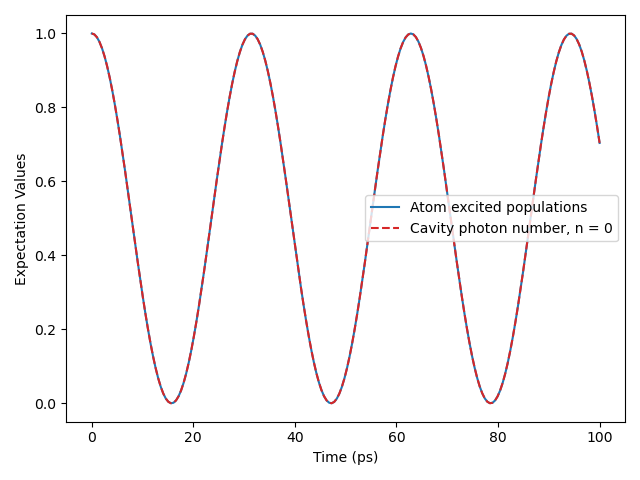
\includegraphics[width=\linewidth]{Research Project/Code/results/JCM/CQS_expt.png}
        \caption{}
        \label{fig:JCM_cqs_xpt_e0}
    \end{subfigure}
    \begin{subfigure}{0.45\textwidth}
        \centering
        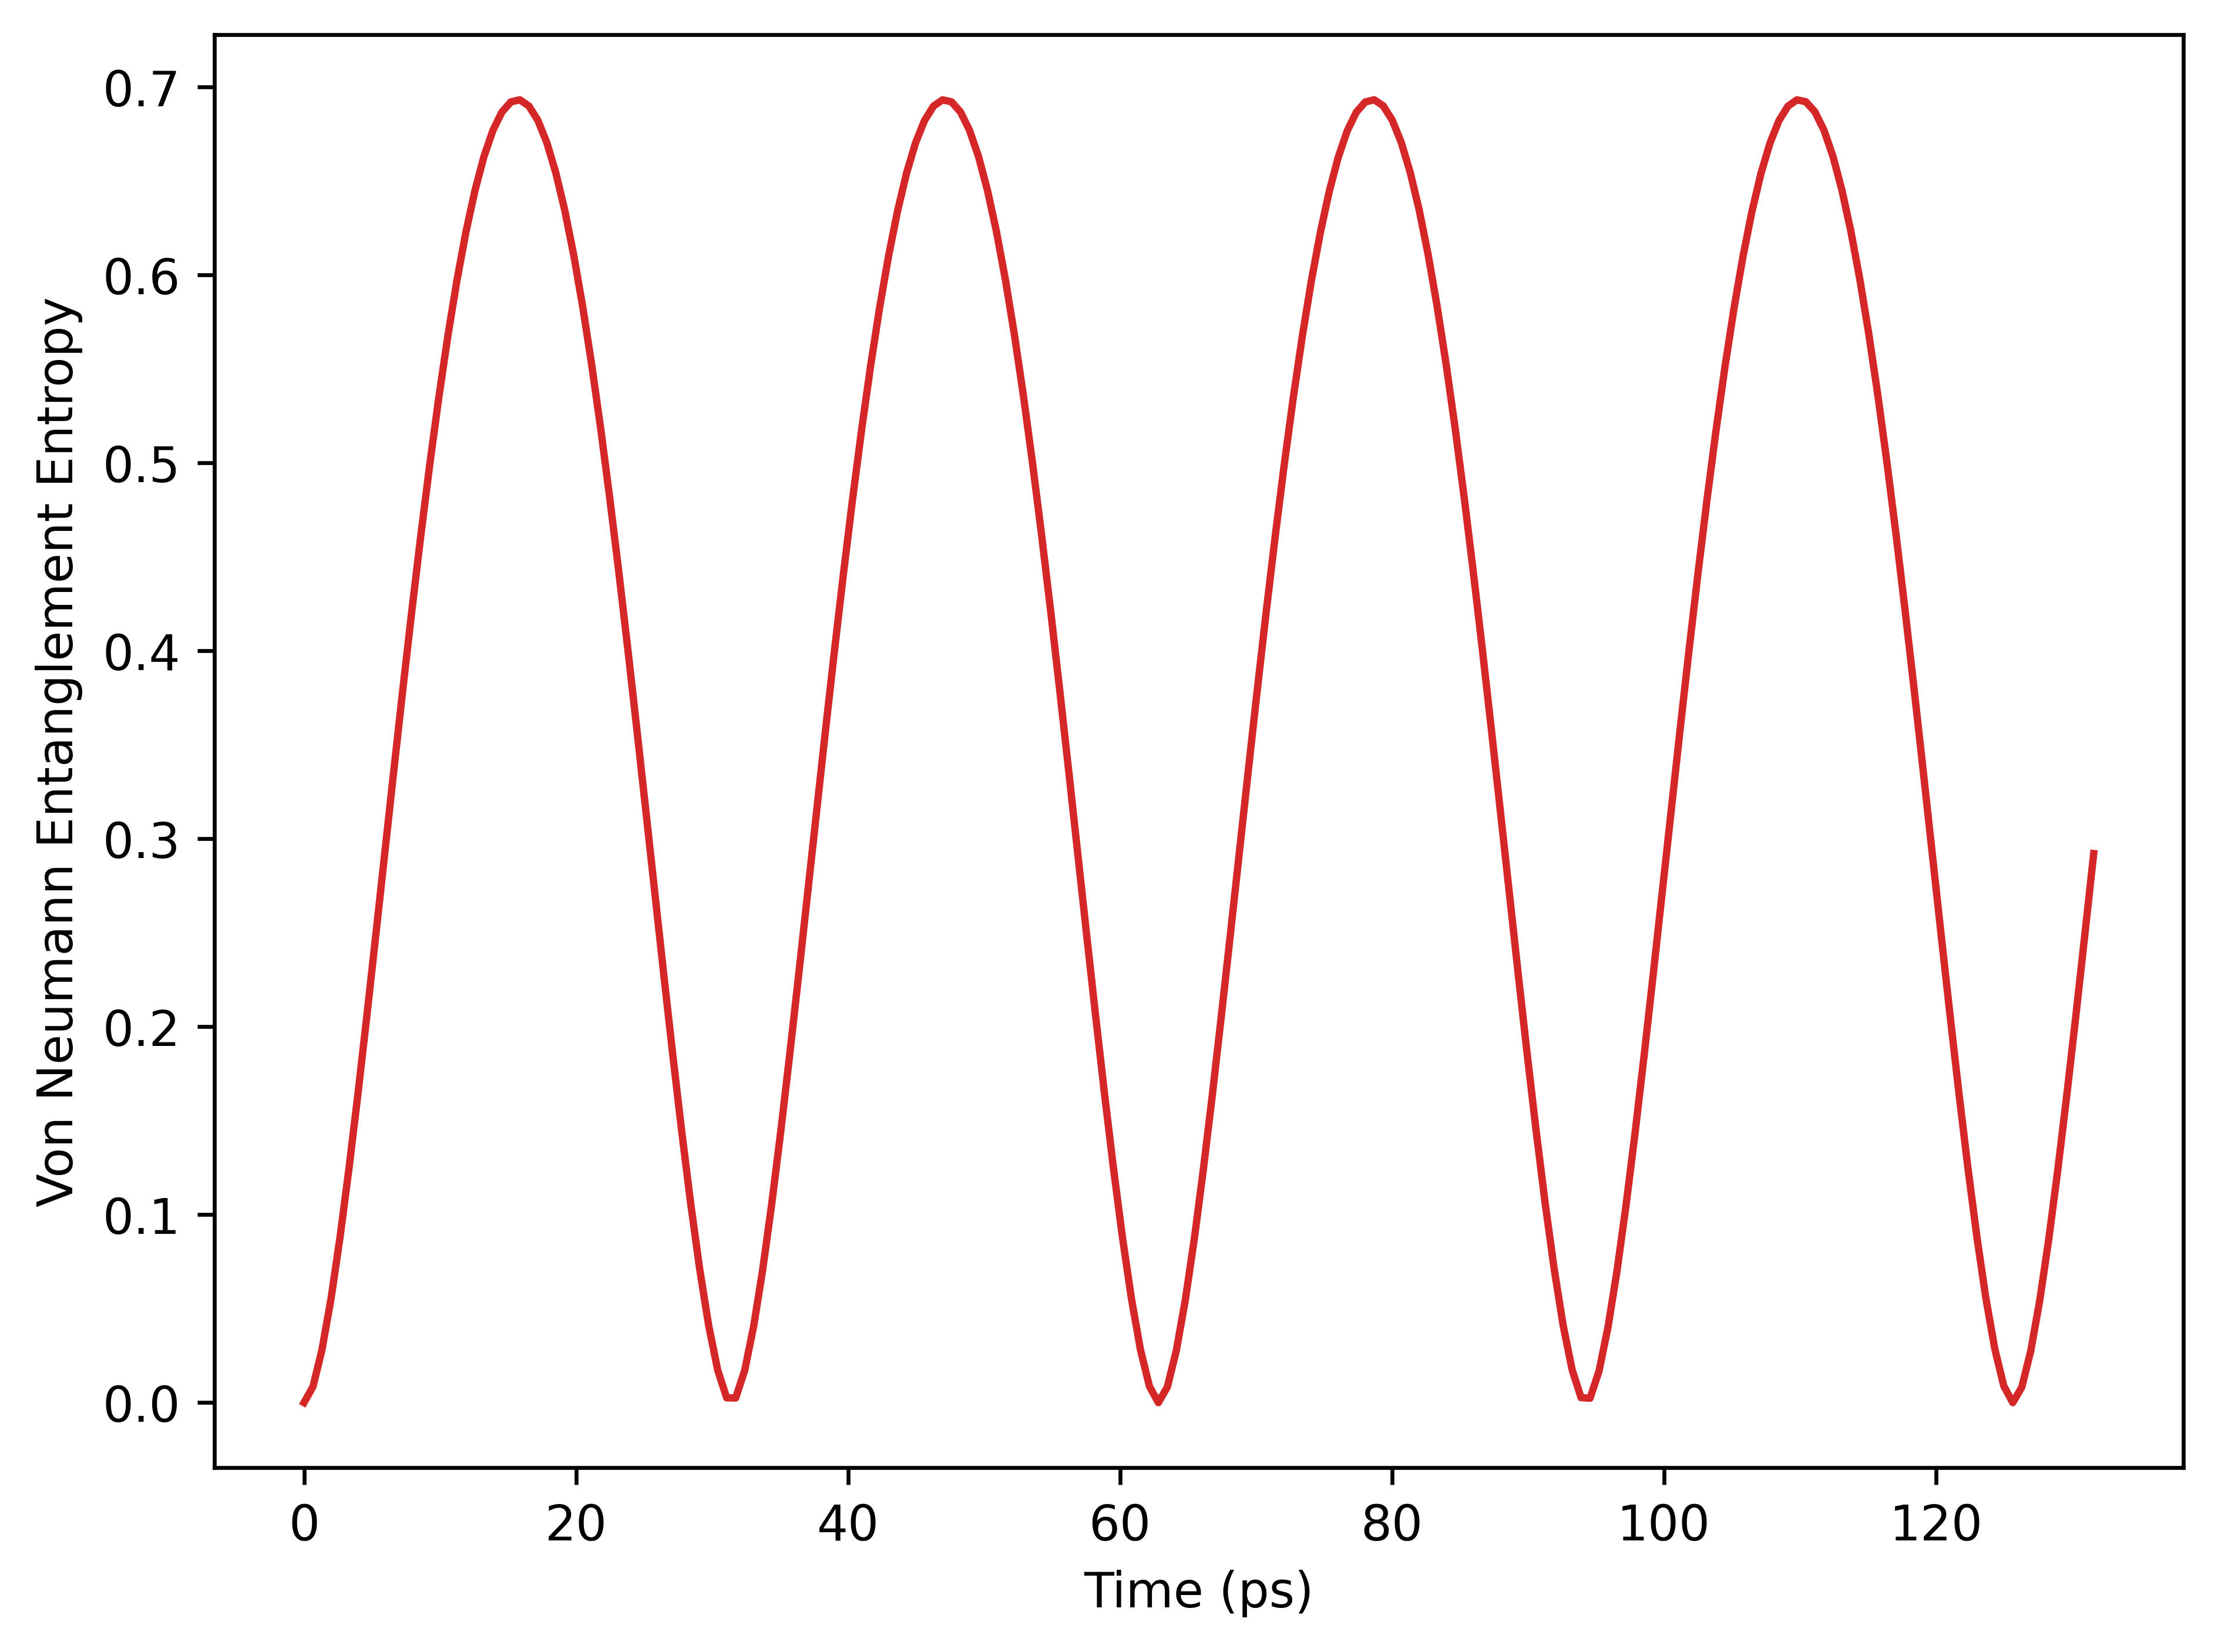
\includegraphics[width=\linewidth]{Research Project/Code/results/JCM/CQS_vne.png}
        \caption{}
        \label{fig:JCM_cqs_vne_e0}
    \end{subfigure}
    
        \vspace{0.5cm}
    
    \begin{subfigure}{0.45\textwidth}
        \centering
        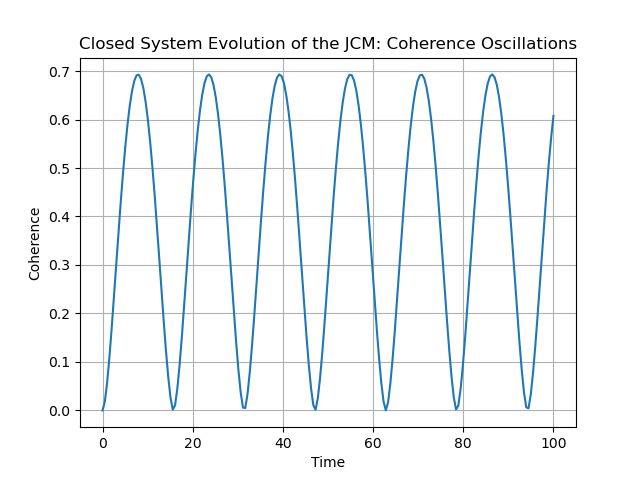
\includegraphics[width=\linewidth]{Research Project/Code/results/JCM/CQS_coh.png}
        \caption{}
        \label{fig:JCM_cqs_coh_e0}
    \end{subfigure}
    \hfill
    \caption{Plots of the JCM under closed unitary evolution with an initial state of $|\psi (\text{t=0})\rangle = |e, 0\rangle$. (a) Populations of the excited atomic state $|e\rangle$, and the cavity state, $|n=1\rangle$. (b) Von Neumann entropy. (c) Relative entropy of coherence for the two subsystems and the total system. For both subsystems, coherence is 0, as indicated by the blue line along the horizontal axis.}
\end{figure}

\noindent In Figure \ref{fig:JCM_cqs_vne_e0}, we observe the Rabi oscillations directly translating into oscillations of entanglement. The periodic transfer of excitation between atom and field drives the von Neumann entropy to cycle between 0 (pure states) and $\ln 2$ (maximal entanglement for a TLS), consistent with our analytical results.\\
\\
When we turn to observe coherence in Figure \ref{fig:JCM_cqs_coh_e0}, there are initially no off-diagonal elements and coherence is thus 0 for the total system. However, as the population begins to transfer between the states $|e,0\rangle,|g,1\rangle$, superpositions of these basis states develop. This produces non-zero off-diagonal terms in the computational basis, corresponding to coherence. The coherence reaches its maximum value of $\ln2$ when the system is in an equal superposition of the basis states, consistent with our theoretical analysis. The Rabi oscillations of the populations are therefore directly responsible for the generation of coherence in the total system of the computational basis. 

\subsubsubsection{Case II: Superposition Initial Condition}

We now carry out our computational analysis of the second initial state from equation \eqref{init_JCM_e0g0}, which reads:

\begin{equation*}
    |\psi (\text{t=0})\rangle = \frac{1}{\sqrt{2}}(|e\rangle + |g\rangle)\otimes|n=0\rangle.
\end{equation*}

\noindent This initial state contains the $|g,0\rangle$ component, which is effectively stationary. In the JCM, the only allowed couplings are between $|e,n\rangle,$ and $|g,n+1\rangle$ due to excitation number conservation. There is no lower photon state for $|g,0\rangle$ couple to,  so it remains unchanged during the evolution. The $|e,0\rangle$ component, however, will evolve in the same manner as the previously considered initial state. We expect that there will be entanglement in the system, since the component $|e,0\rangle$ will, during its transition into the $|g,1\rangle$, be in some linear combination of $|e,0\rangle$ and $|g,1\rangle$. We also anticipate that both the subsystems and the total system will exhibit coherence, as the initial state is a superposition. Consequently, the subsystems should contain off--diagonal terms.\\
\begin{figure}[h]
    \centering
    \begin{subfigure}{0.45\textwidth}
        \centering
        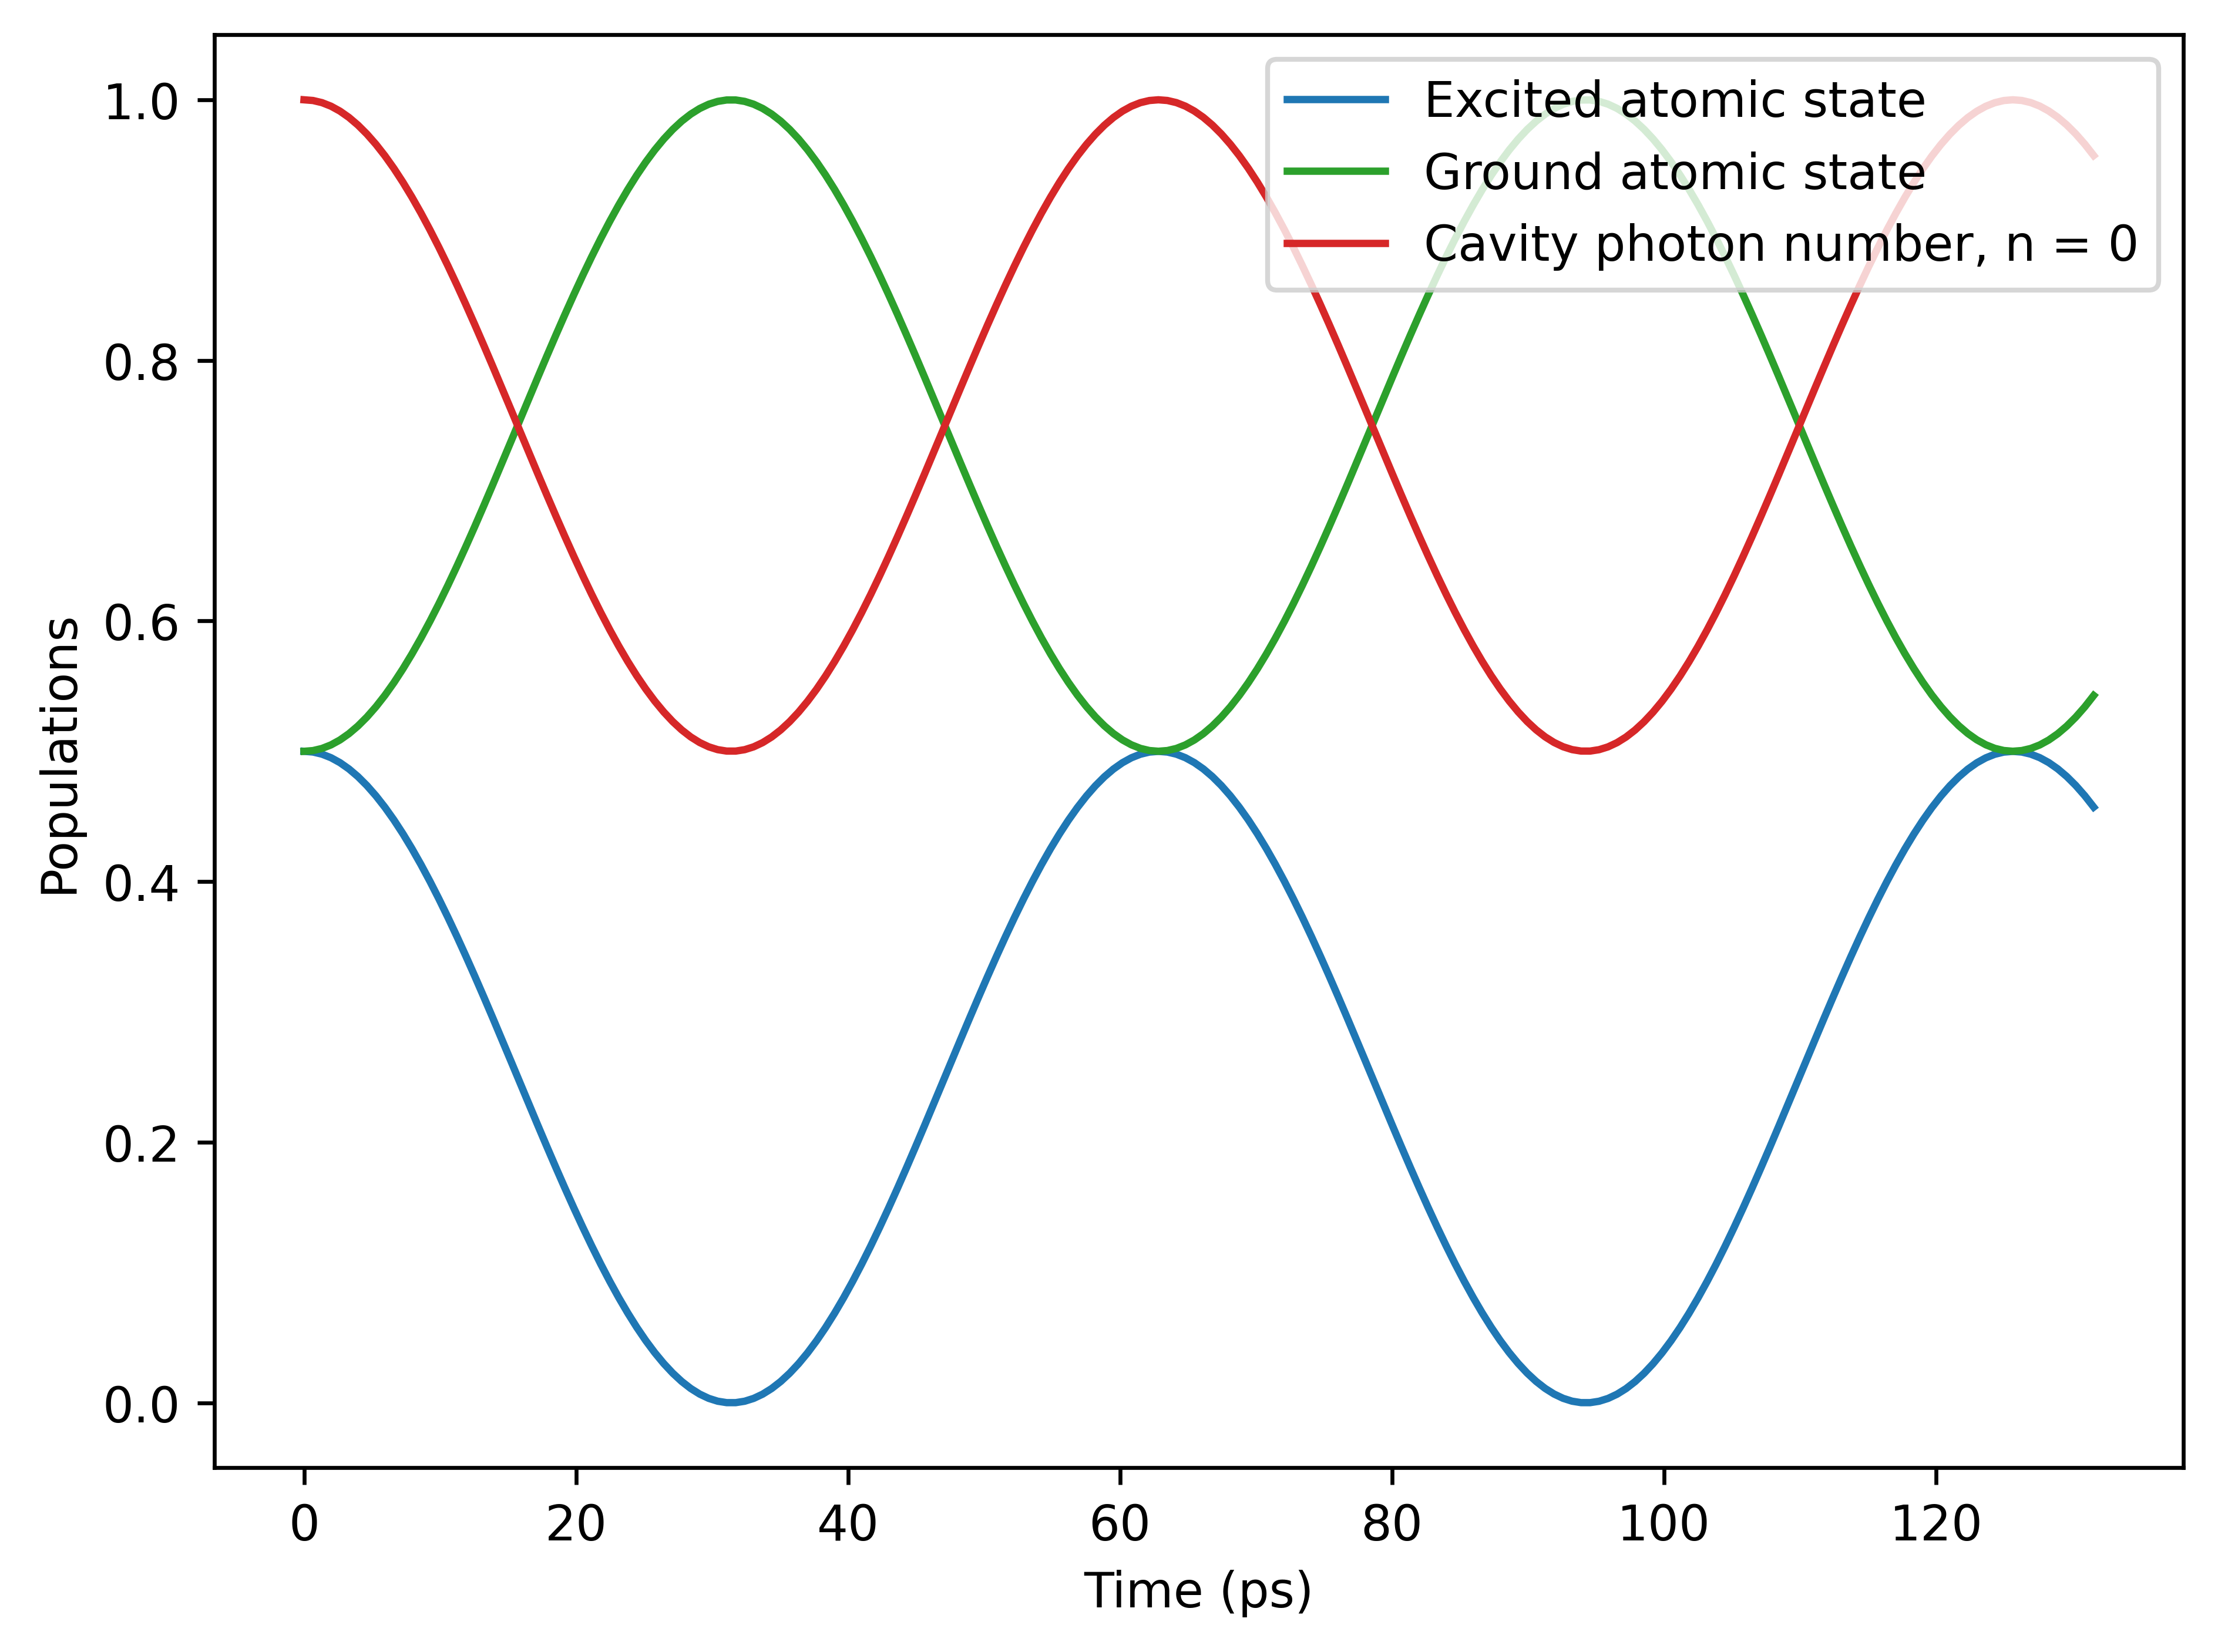
\includegraphics[width=\linewidth]{Research Project/Code/results/JCM/CQS_expt_eg.png}
        \caption{}
        \label{fig:jcm_cqs_expt_eg}
    \end{subfigure}
    \hfill
    \begin{subfigure}{0.45\textwidth}
        \centering
        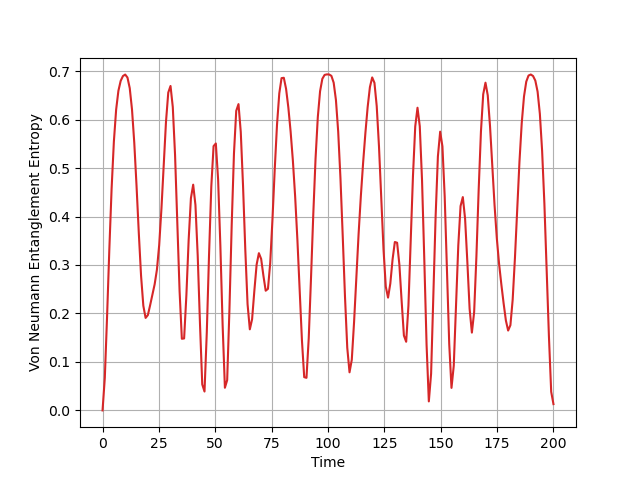
\includegraphics[width=\linewidth]{Research Project/Code/results/JCM/CQS_vne_eg.png}
        \caption{}
        \label{fig:jcm_cqs_vne_eg}
    \end{subfigure}
    
    \vspace{0.5cm}
    
    \begin{subfigure}{0.45\textwidth}
        \centering
        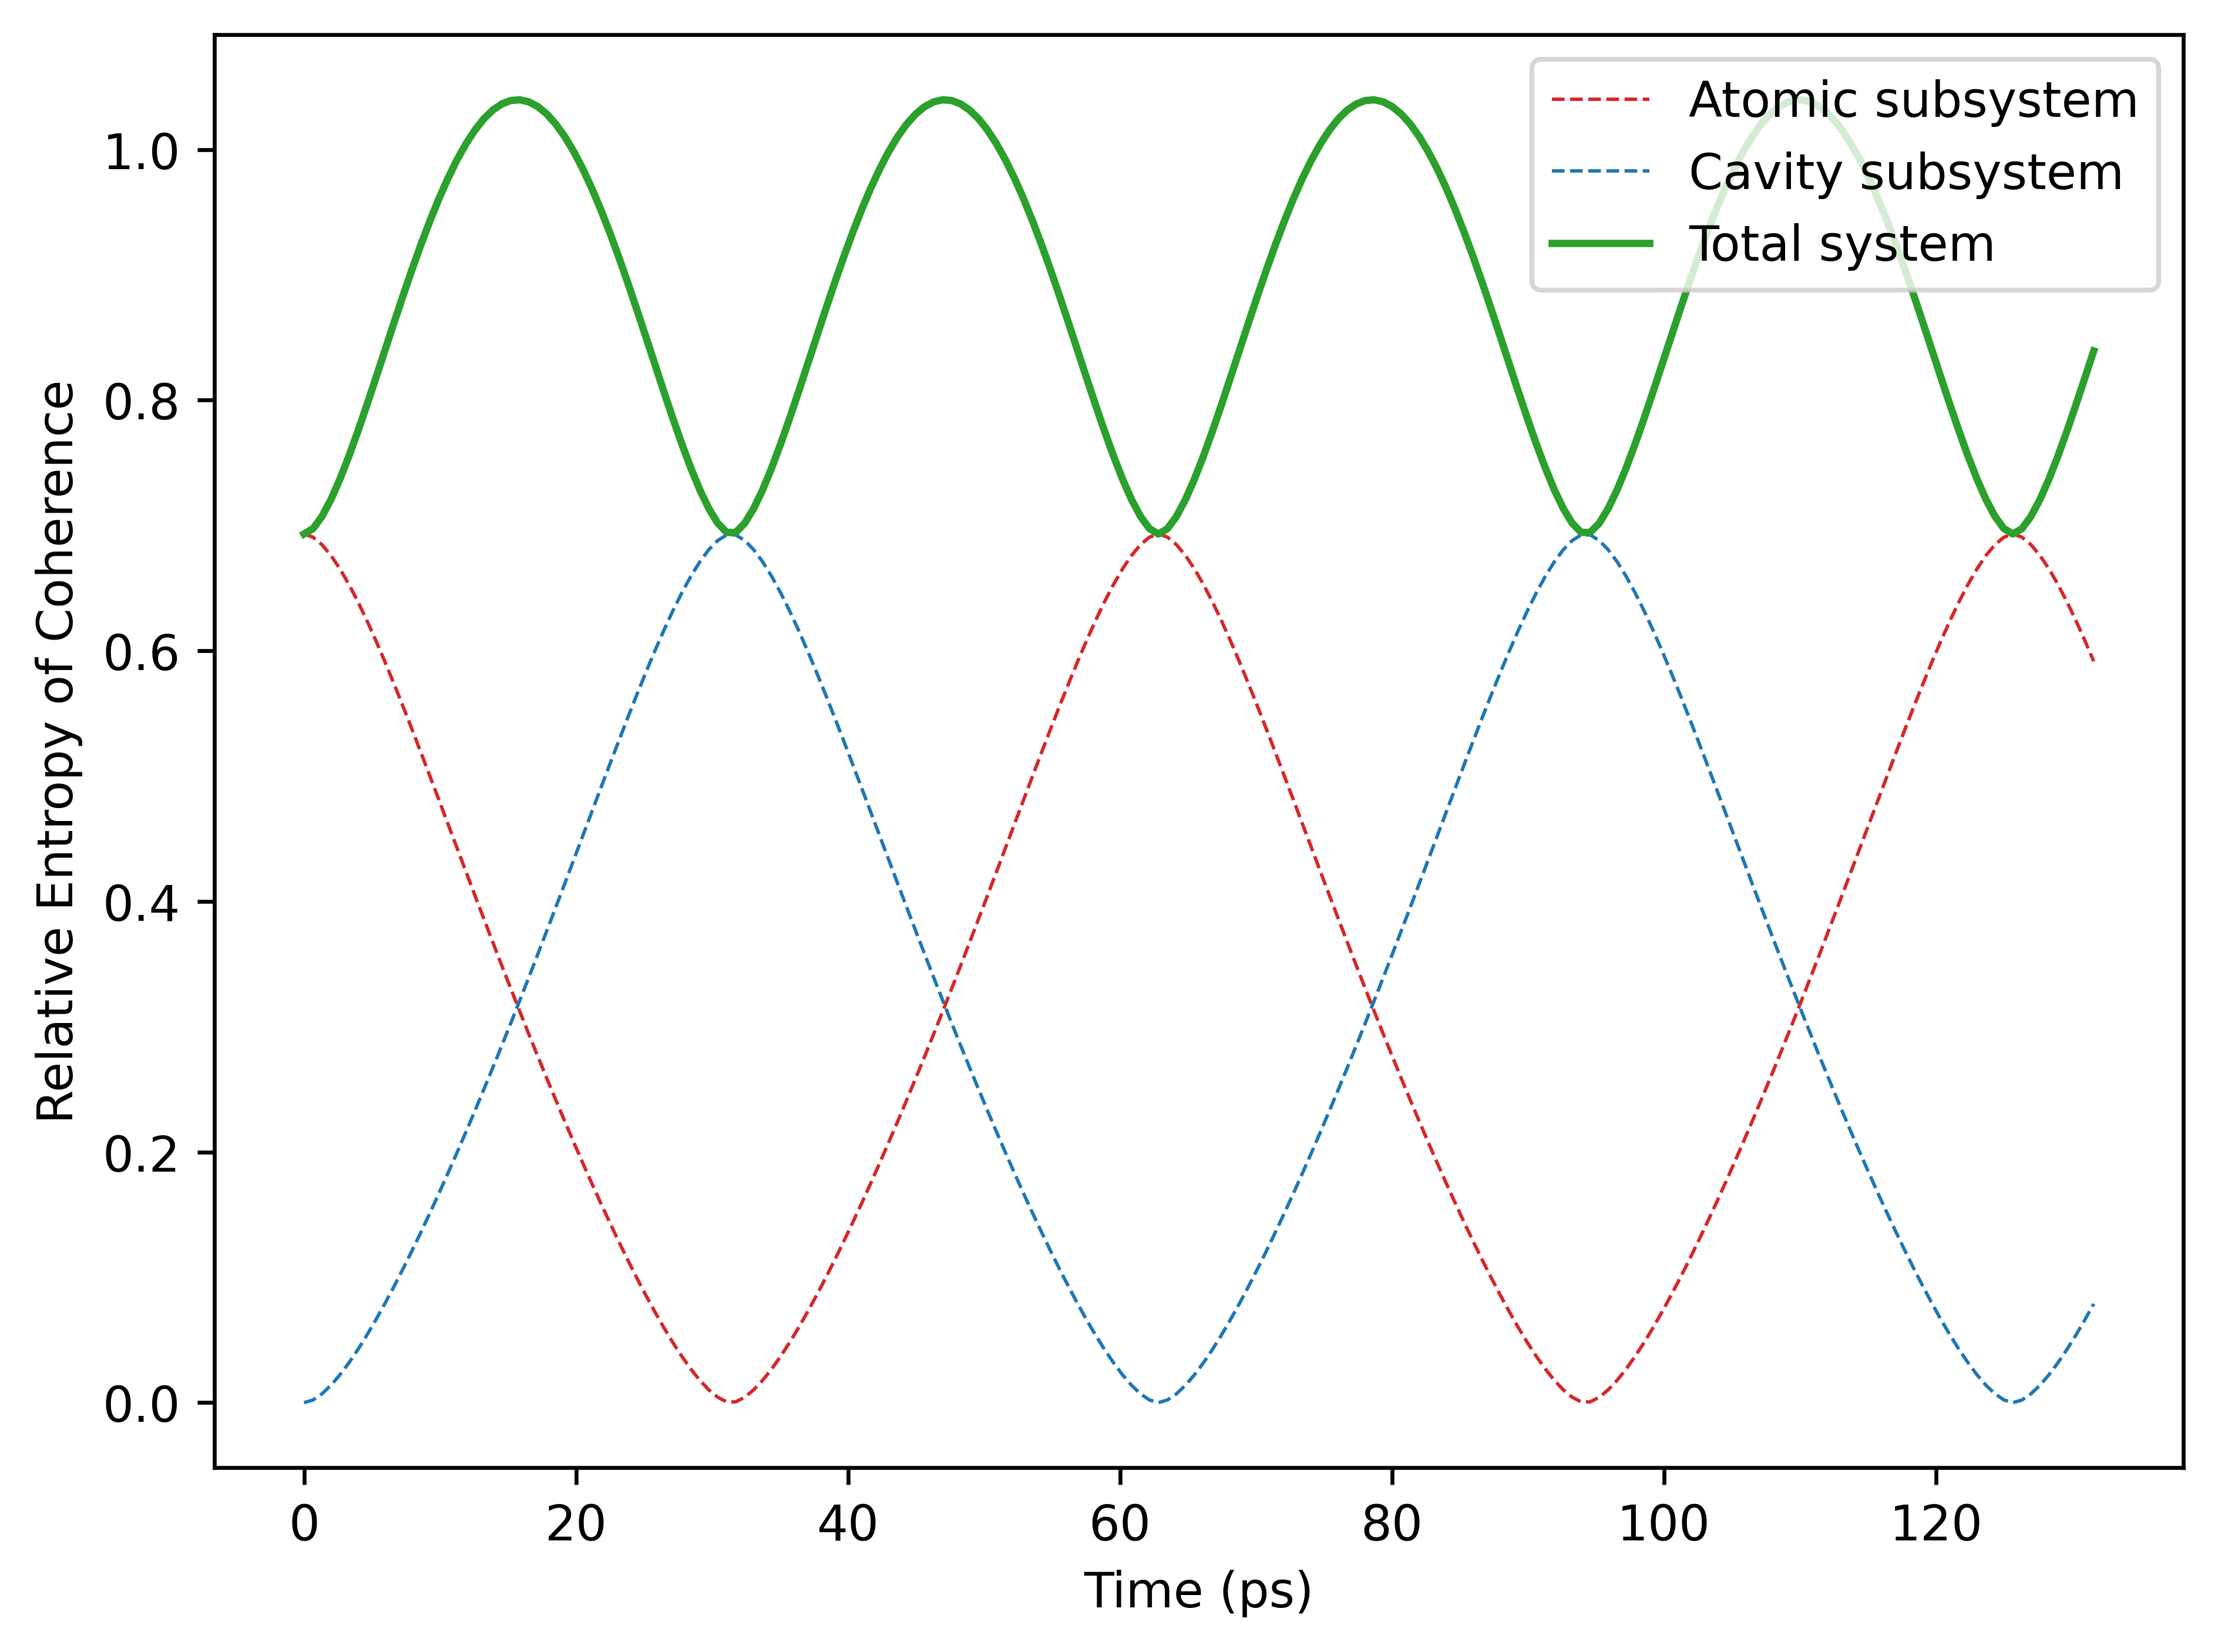
\includegraphics[width=\linewidth]{Research Project/Code/results/JCM/CQS_coh_eg.png}
        \caption{}
        \label{fig:jcm_cqs_coh_eg}
    \end{subfigure}
    \hfill

    \caption{Plots of the JCM under closed unitary evolution with an initial state of $|\psi (\text{t=0})\rangle = 1/\sqrt{2}(|e\rangle + |g\rangle)\otimes|n=0\rangle$. (a) Populations of the excited atomic state $|e\rangle$, the ground atomic state $|g\rangle$ and the cavity state, $|n=0\rangle$. (b) Von Neumann entropy. (c) Relative entropy of coherence for the two subsystems and the total system.}
    \label{fig:JCM_cqs_e0g0}
\end{figure}

\noindent We start by analysing Figure \ref{fig:jcm_cqs_expt_eg}, which shows the populations of the ground and excited state of the atom, and the cavity state population of the $|n=0\rangle$ Fock state. As expected, the $|g,0\rangle$ component of the initial state is stationary, and so there will always be a non-zero contribution to the populations of $|g\rangle$ and $|n=0\rangle$. At $t\approx 30\text{ps}$, we see that half the population of the cavity is transferred to $|n=1\rangle$, and for the atom, to $|g\rangle$. This illustrates the expected Rabi oscillation dynamics, where the excitation initially in the $|e,0\rangle$ state is transferred coherently to the $|g,1\rangle$ state. \\
\\
As expected, there is entanglement in the system, characterised by the von Neumann entropy (Figure \ref{fig:jcm_cqs_vne_eg}). It exhibits the same oscillations as the previous initial state's entanglement characteristics due to the Rabi oscillations in the populations. Furthermore, entanglement is maximal during the transition of the $|e,0\rangle$ component to $|g,1\rangle$ which matches our predictions. However, the range of entanglement is much lower (between 0 and 0.25 as compared to 0 and 0.7 in Figure \ref{fig:JCM_cqs_vne_e0}. This could be attributed to entanglement being diluted by the $|g,0\rangle$ component. The $|g,0\rangle$ component remains stationary, never mixes with the other components, and effectively behaves as an unentangled product state.
In terms of the von Neumann entropy, this stationary, classically--behaving fraction of the total state limits the entanglement achieved during evolution.\\
\\
Finally, we observe coherence in the full system, $C_r(\rho(t))$. Although this behaviour resembles that of our previous initial condition,  the presence of the stationary component leads to some key differences. The stationary component $|g,0\rangle$ adds an off--diagonal term to our full system, thus creating a baseline level of coherence throughout the evolution. This causes the minimum of $C_r(\rho(t))$ is approximately 0.5, whereas previously it was 0. Moreover, it raises the maximum value of $C_r(\rho(t))$. We also observe coherences in both subsystems. To see why there is coherence in the initial state for the atomic subsystem, but not the cavity subsystem, let us analyse the initial condition's subsystems.

\begin{equation*}
    |\psi (\text{t=0})\rangle = \frac{1}{\sqrt{2}}(|e\rangle + |g\rangle)\otimes|n=0\rangle,
\end{equation*}

so its density matrix is

\begin{equation*}
    |\rho(t=0)\rangle = \frac{1}{2}\left(|e,0\rangle\langle e,0| + |g,0\rangle\langle g,0| + |e,0\rangle\langle g,0| + |g,0\rangle\langle e,0| \right).
\end{equation*}

The atomic subsystem is found by taking the partial trace:

\begin{equation*}
    \rho_{\scriptscriptstyle \text{TLS}}(t = 0) = \frac{1}{2}\left(|e\rangle\langle e|+ |g\rangle\langle g|+|e\rangle\langle g|+|g\rangle\langle e|\right),
\end{equation*}

and so we expect there to be coherence in this subsystem initially. For the cavity subsystem, however, 

\begin{equation*}
    \rho_{\scriptscriptstyle \text{QHO}}(t = 0) = \left(|0\rangle\langle 0|\right),
\end{equation*}

which is a diagonal matrix and thus has no coherence at t=0. The coherence values for each subsystem oscillates between 0 and 0.7, which matches our expectations due to the population transfers caused by Rabi oscillations.\\
\\
We observe an important effect of this initial condition on the coherence and entanglement of the system. While the presence of the stationary $|g,0\rangle$ component enhances coherence, it simultaneously reduces the maximum amount of entanglement generated. This trade--off emphasises the sensitivity of coherence and entanglement to the initial state: introducing a pure, unentangled state with a superposition can increase the overall coherence, but only at the cost of reduced entanglement.\\
\\
Having analysed the coherence and population dynamics under closed evolution, we now turn to open system dynamics, where the interaction with the environment is included via the Lindblad formalism. This allows us to explore how decoherence and dissipation affect the behaviour observed in the closed system.

\subsubsection{Open Evolution}
\subsubsubsection{Case I: Excited State Initial Condition}
We start our analysis of open quantum evolution by considering our first initial state in equation \eqref{init_JCM_e0}.

\begin{figure}[H]
    \centering
    \begin{subfigure}{0.45\textwidth} 
        \centering
        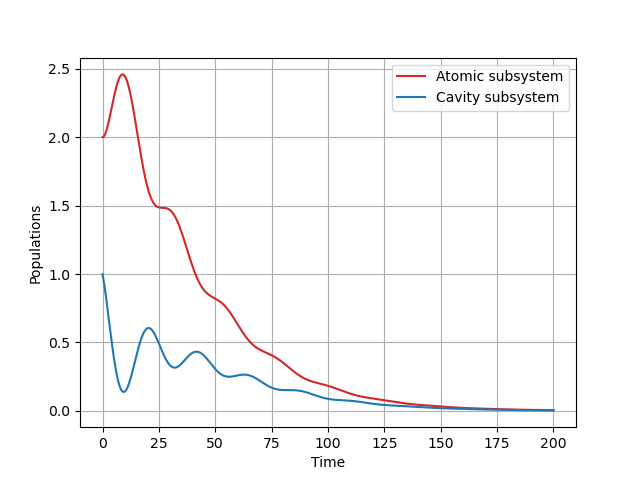
\includegraphics[width=\linewidth]{Research Project/Code/results/JCM/OQS_Pop_Spont.png}
        \caption{}
        \label{fig:JCM_OQS_Pop_Spont}
    \end{subfigure}
    \hfill
    \begin{subfigure}{0.45\textwidth}
        \centering
        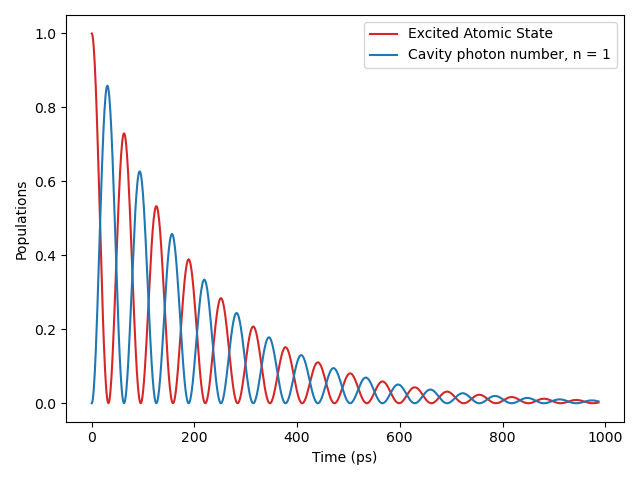
\includegraphics[width=\linewidth]{Research Project/Code/results/JCM/OQS_Pop_Therm.png}
        \caption{}
         \label{fig:JCM_OQS_Pop_Therm}
    \end{subfigure}
    
    \vspace{0.5cm}
    
    \begin{subfigure}{0.45\textwidth} 
        \centering
        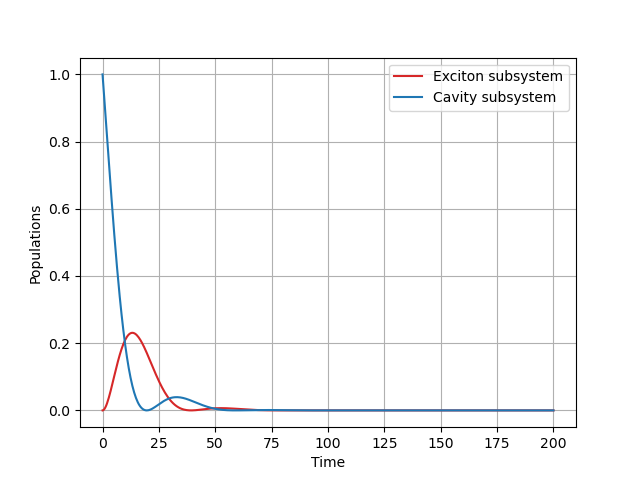
\includegraphics[width=\linewidth]{Research Project/Code/results/JCM/OQS_Pop_Both.png}
        \caption{}
         \label{fig:JCM_OQS_Pop_Both}
    \end{subfigure}
    \hfill
    \caption{Plots of the JCM subsystem populations under open system evolution, with an initial state of $|\psi (\text{t=0})\rangle = |e, 0\rangle$. (a) Evolution under spontaneous atomic emission. (b) Evolution under thermal dissipation. (c) Evolution under both spontaneous atomic emission and thermal dissipation.}
    \label{fig:JCM_OQS_Pop}
\end{figure}

\noindent Under all types of decay (see Section \ref{sec:method_sub_JCM}), we observe Rabi oscillations as expected. However, the populations of both subsystems dissipate due to losses to the environment, a hallmark of open quantum evolution. Interestingly, the Rabi oscillation period remains constant over all time, since the Rabi frequency $g$ is time--independent. Figures \ref{fig:JCM_OQS_Pop_Spont}, \ref{fig:JCM_OQS_Pop_Therm} further show that the decay of both subsystems under either spontaneous atomic emission and thermal dissipation are almost identical. We can attribute this similarity to the low--temperature regime, where thermal dissipation is effectively reduced to photon loss (see equation \eqref{eqn:L_therm}). Thus, the decay operator for the dissipator is effectively only photon loss. Moreover, since we set the decay rates of the thermal and spontaneous emission to be equal ($\gamma = \gamma_{\scriptscriptstyle \text{th}} =0.01$, the two decay channels act in essentially the same way, just on different subsystems. The Rabi oscillations themselves also mediate decay between subsystems via excitation transfer, a key characteristic of the JCM. Finally, while the isolated decay channels drive the populations to their ground state around $t = 1000 ps$, when both channels are open simultaneously, we observe a decay timescale of about $t = 600 ps$ (Figure \ref{fig:JCM_OQS_Pop_Both}). 

\begin{figure}[H]
    \centering
    \begin{subfigure}{0.45\textwidth}
        \centering
        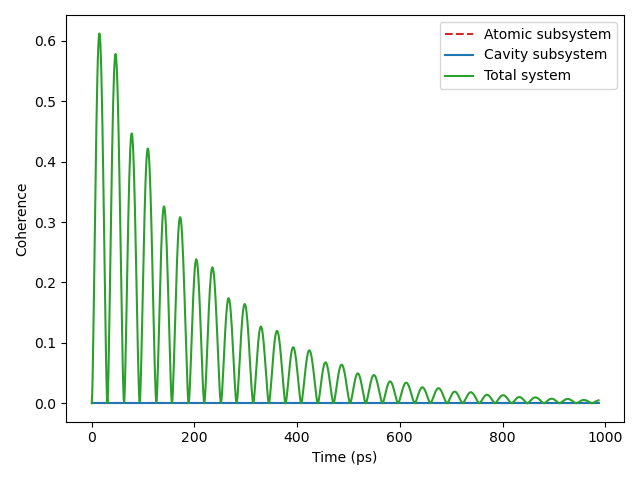
\includegraphics[width=\linewidth]{Research Project/Code/results/JCM/OQS_Coh_Spont.png}
        \caption{}
        \label{fig:JCM_OQS_Coh_Spont}
    \end{subfigure}
    \hfill
    \begin{subfigure}{0.45\textwidth}
        \centering
        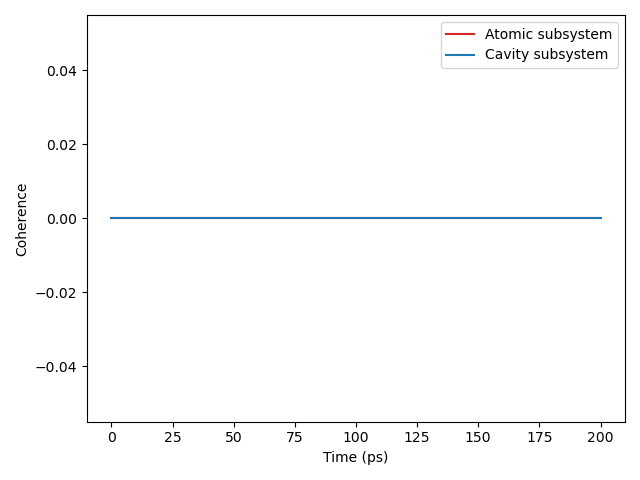
\includegraphics[width=\linewidth]{Research Project/Code/results/JCM/OQS_Coh_Therm.png}
        \caption{}
        \label{fig:JCM_OQS_Coh_Therm}
    \end{subfigure}
    
    \vspace{0.5cm}
    
    \begin{subfigure}{0.45\textwidth}
        \centering
        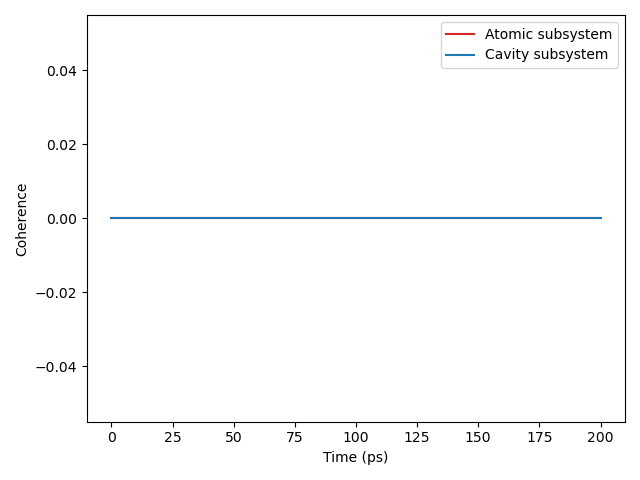
\includegraphics[width=\linewidth]{Research Project/Code/results/JCM/OQS_Coh_Both.png}
        \caption{}
        \label{fig:JCM_OQS_Coh_Both}
    \end{subfigure}
    \hfill
    \caption{Plots of the decay of coherence (decoherence) of the JCM under open system evolution using the relative entropy of coherence measure, with an initial state of $|\psi (\text{t=0})\rangle = |e, 0\rangle$. Both subsystems have a coherence of 0, indicated by the blue line along the horizontal axis. (a) Decoherence under spontaneous atomic emission. (b) Decoherence under thermal dissipation. (c) Decoherence under both spontaneous atomic emission and thermal dissipation.}
    \label{fig:JCM_OQS_Coh}
\end{figure}

\noindent When discussing open quantum systems, a defining feature of such evolution is decoherence, which, as noted in Section \ref{sec:theory_sub_OQS}, corresponds to the decay of off--diagonals elements of the density matrix, leading to a loss of 'quantumness'. We can observe this directly by tracking the decay of coherence. In the computational basis $\{|e,0\rangle, |g,1\rangle\}$, closed evolution exhibits coherence for the total system, so we expect coherence to be present under open system evolution as well. We indeed observe this. For all types of decay, the total system's coherence decays on the same timescales as the populations: around $t \approx 1000ps$ for spontaneous emission and thermal dissipation (Figures \ref{fig:JCM_OQS_Coh_Spont}, \ref{fig:JCM_OQS_Coh_Therm}), and $ t \approx 600ps$ when both decay channels are active simultaneously (Figure \ref{fig:JCM_OQS_Coh_Both}). Since Lindblad operators remove excitations, they suppress both diagonal and off--diagonal elements of the density matrix on comparable timescales. Thus, in this basis, coherence cannot outlive population, so both decay together. \\
\\
To conclude our simulations of the JCM, we examine the system's entanglement via the negativity measure. Figure \ref{fig:JCM_OQS_Neg} shows that negativity decays on a timescale roughly twice as fast as the population for all types of decay. This can be understood by noting that entanglement requires simultaneous occupation of both states $|e,0\rangle$ and $|g,1\rangle$. Consider, for instance, the spontaneous emission channel. For entanglement to persist, both states must remain populated. However, spontaneous emission acts directly damps the excited atomic state $|e,0\rangle$.  and through Rabi oscillations, the $|g,1\rangle$ state is also gradually depleted. Thus, the superposition of both states decays twice as fast, resulting in the observed doubling of decay rate for entanglement. A similar process occurs under the thermal dissipation, except that the single photon state $|g,1\rangle$ is directly damped by photon loss, and
\begin{figure}[H] 
    \centering
    \begin{subfigure}{0.45\textwidth}
        \centering
        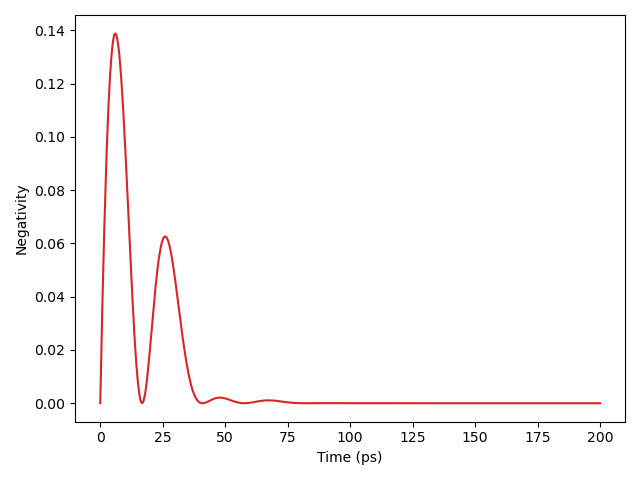
\includegraphics[width=\linewidth]{Research Project/Code/results/JCM/OQS_Neg_Spont.png}
        \caption{}
        \label{fig:JCM_OQS_Neg_Spont}
    \end{subfigure}
    \hfill
    \begin{subfigure}{0.45\textwidth}
        \centering
        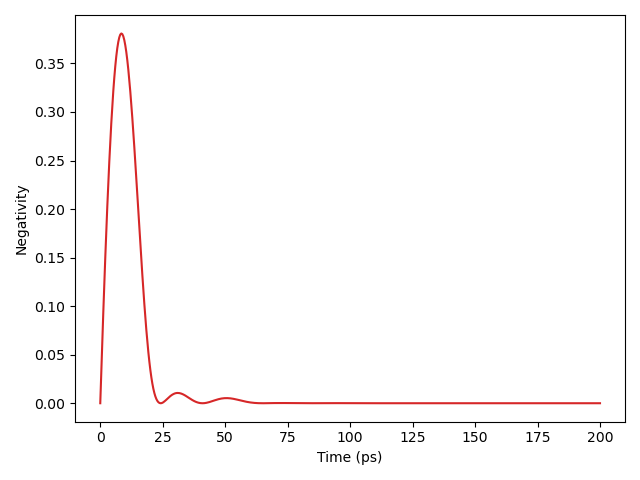
\includegraphics[width=\linewidth]{Research Project/Code/results/JCM/OQS_Neg_Therm.png}
        \caption{}
        \label{fig:JCM_OQS_Neg_Therm}
    \end{subfigure}
    
    \vspace{0.5cm}
    
    \begin{subfigure}{0.45\textwidth}
        \centering
        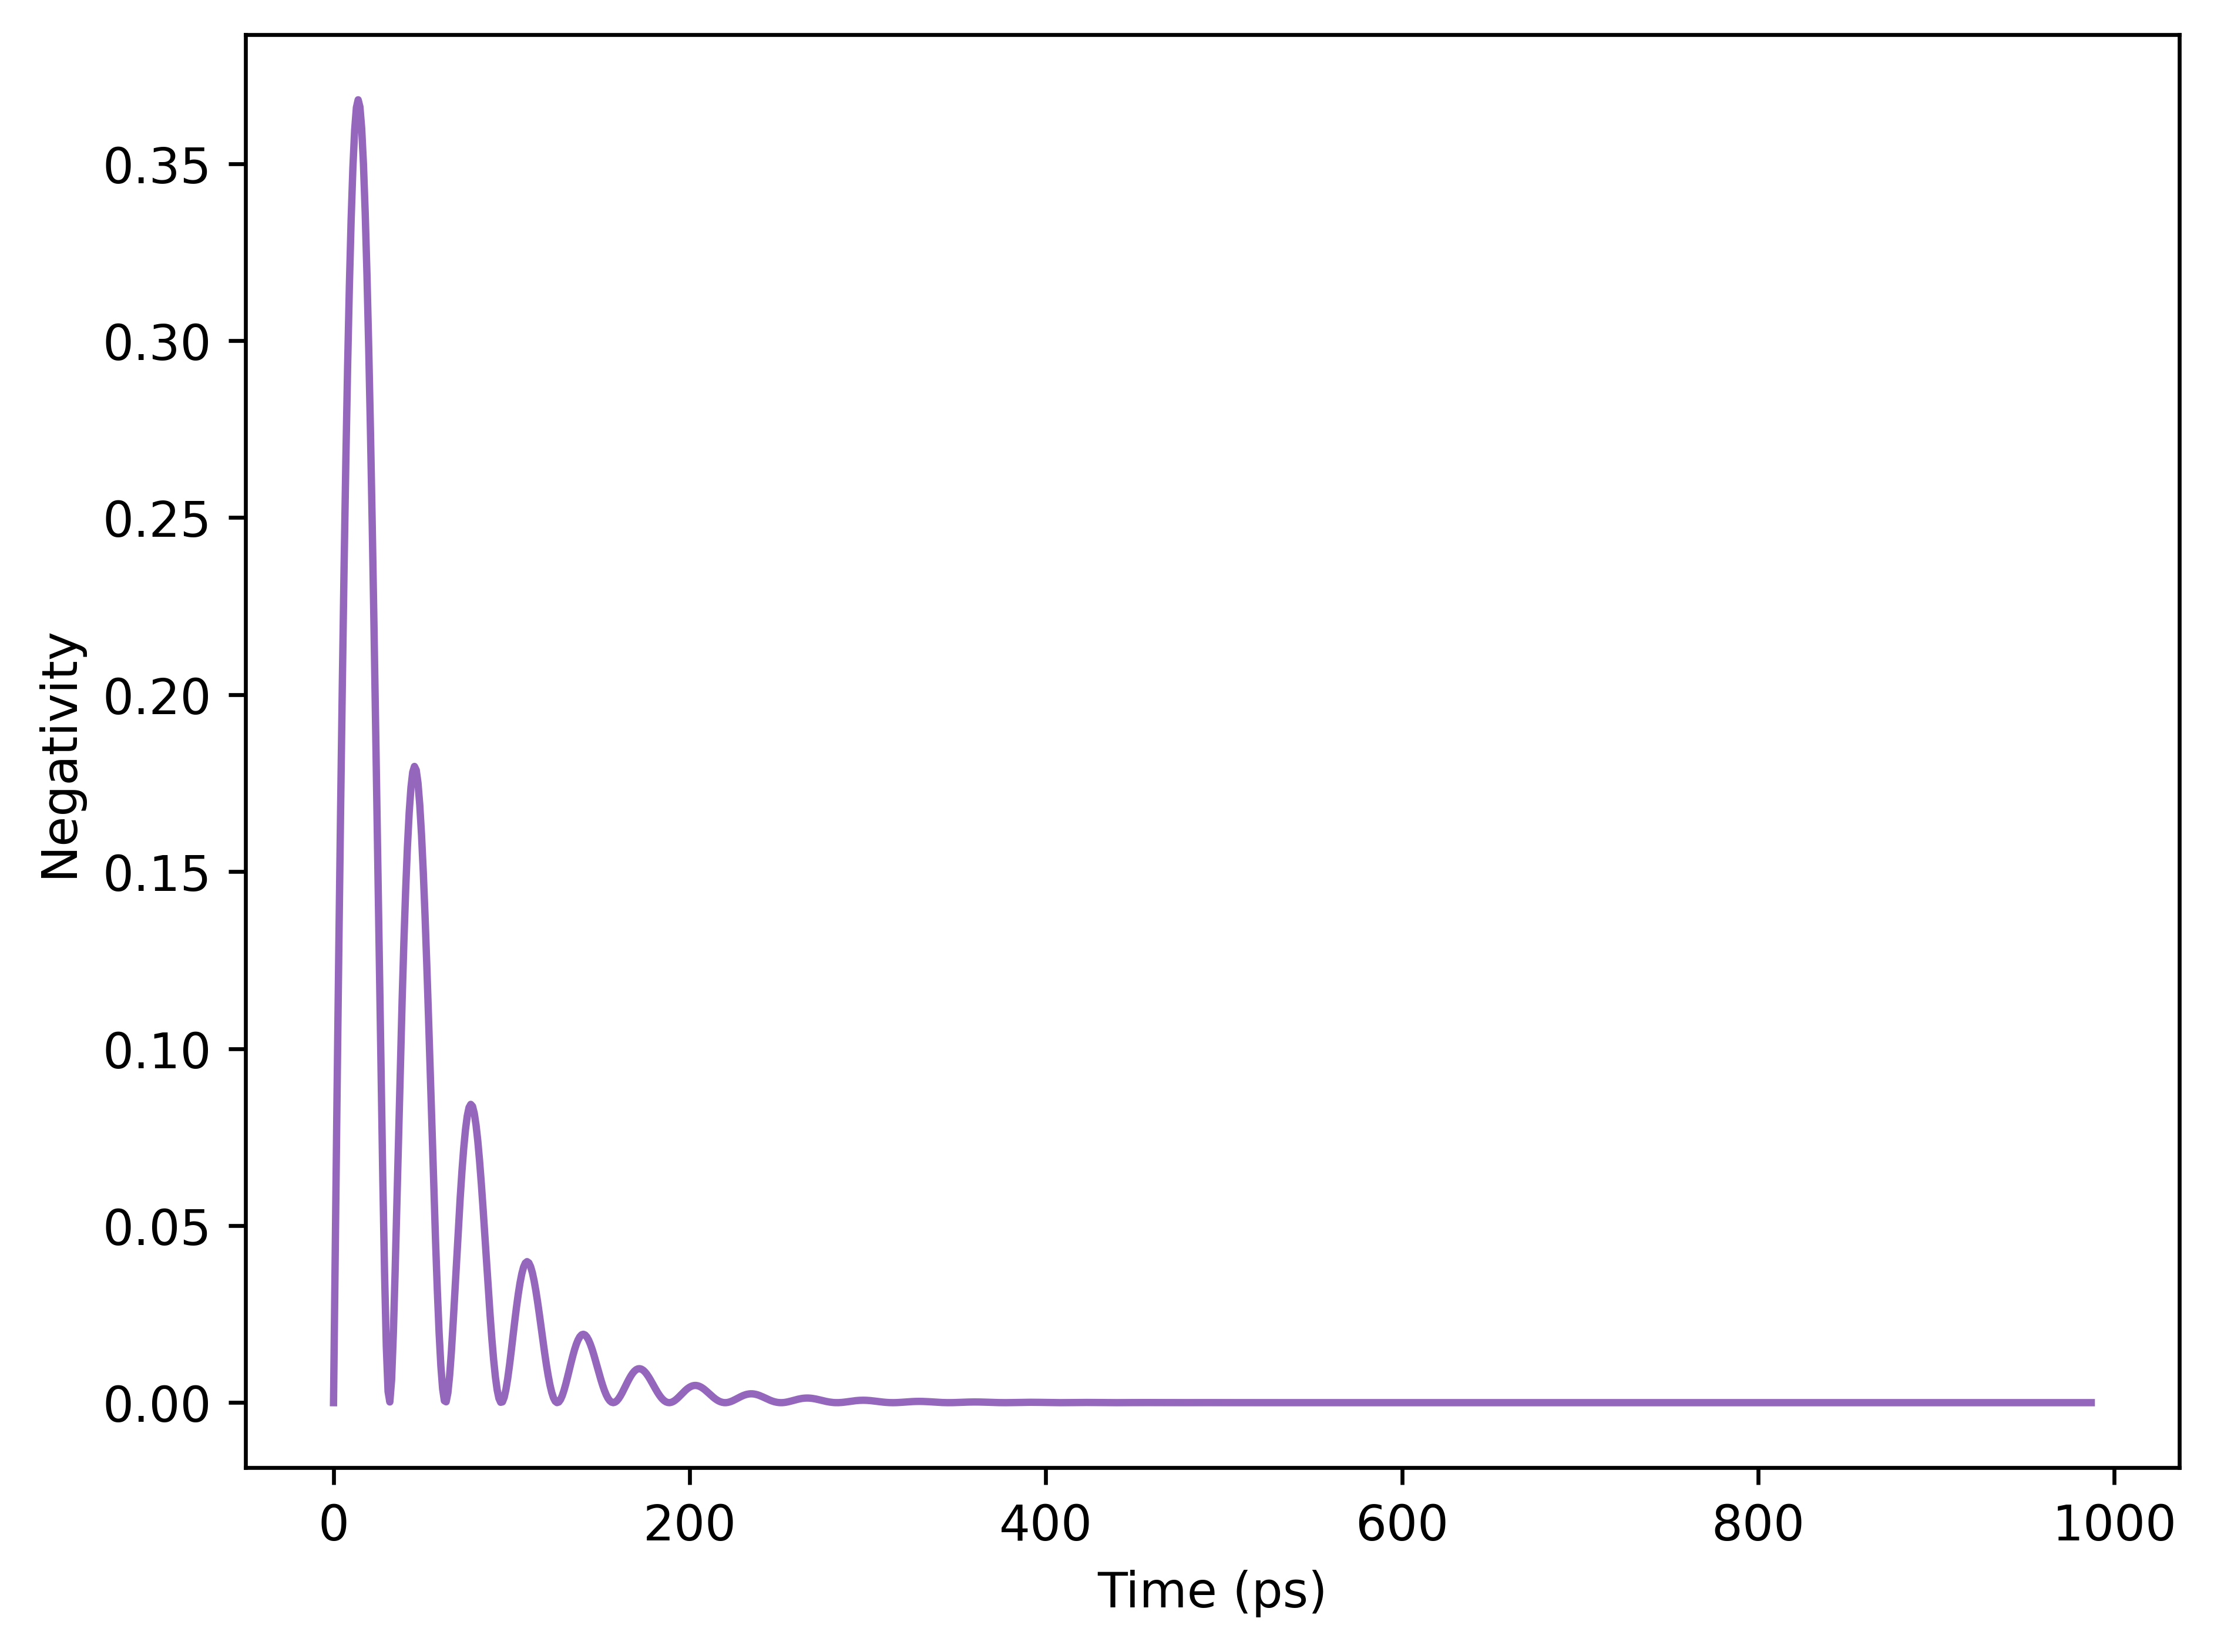
\includegraphics[width=\linewidth]{Research Project/Code/results/JCM/OQS_Neg_Both.png}
        \caption{}
        \label{fig:JCM_OQS_Neg_Both}
    \end{subfigure}
    \hfill
    \caption{Plots of the decay of entanglement of the JCM under open system evolution using the negativity measure, with an initial state of $|\psi (\text{t=0})\rangle = |e, 0\rangle$. (a) Entanglement decay under spontaneous atomic emission. (b) Entanglement decay under thermal dissipation. (c) Entanglement decay under both spontaneous atomic emission and thermal dissipation.}
    \label{fig:JCM_OQS_Neg}
\end{figure}

\noindent through Rabi oscillations the $|e,0\rangle$ component is likewise suppressed. When both decay channels are open (Figure \ref{fig:JCM_OQS_Neg_Both}), we observe a decay time that is approximately halved compared to either channel acting alone. This behaviour highlights a key way in which entanglement manifests in TLS--QHO systems: it is generated by Rabi oscillations, but is particularly fragile to environmental loss, decaying more rapidly than populations themselves. In contrast to coherence and population oscillations, which persist on comparable timescales, entanglement emerges as a more vulnerable quantum resource, setting a fundamental limit on how such systems may be exploited for quantum information tasks.

\subsubsubsection{Case II: Superposition Initial Condition}

As with the closed simulation, we also consider the second initial state in equation \eqref{init_JCM_e0g0}.\\
\\
Figure \ref{fig:JCM_OQS_Pop_eg} shows that the populations decay at the same rate as in the previous initial condition (Figure \ref{fig:JCM_OQS_Pop}) for all decay channel types. This is expected, since we use the same decay parameters ($\gamma= \gamma_{\scriptscriptstyle \text{th}} = 0.01$). The only difference is that the population for the excited atomic state is 0.5, consistent with the initial state being an equal superposition of the $|e\rangle$ and $|g\rangle$ coupled to the $|n=0\rangle$ Fock state of the cavity. \\


\begin{figure}[H]
    \centering
    \begin{subfigure}{0.45\textwidth}
        \centering
        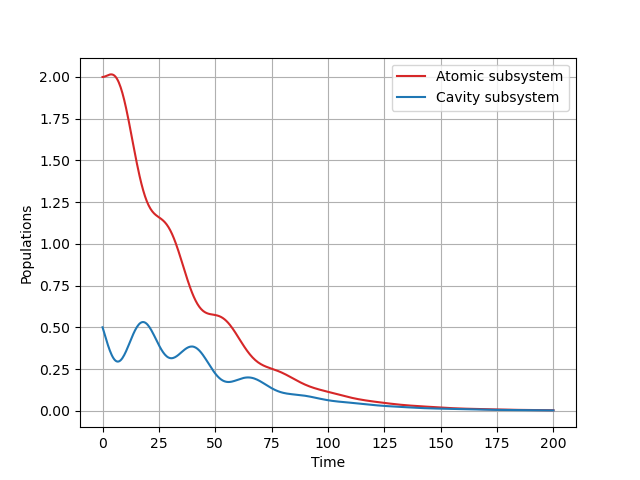
\includegraphics[width=\linewidth]{Research Project/Code/results/JCM/OQS_Pop_Spont_eg.png}
        \caption{}
        \label{fig:JCM_OQS_Pop_Spont_eg}
    \end{subfigure}
    \hfill
    \begin{subfigure}{0.45\textwidth}
        \centering
        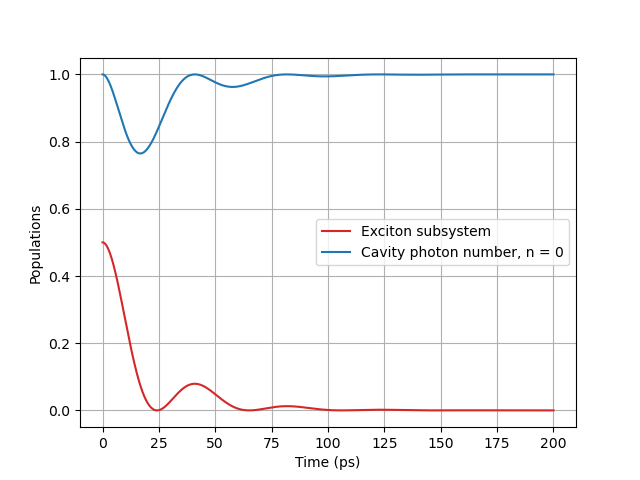
\includegraphics[width=\linewidth]{Research Project/Code/results/JCM/OQS_Pop_Therm_eg.png}
        \caption{}
        \label{fig:JCM_OQS_Pop_Therm_eg}
    \end{subfigure}
    
    \vspace{0.5cm}
    
    \begin{subfigure}{0.45\textwidth}
        \centering
        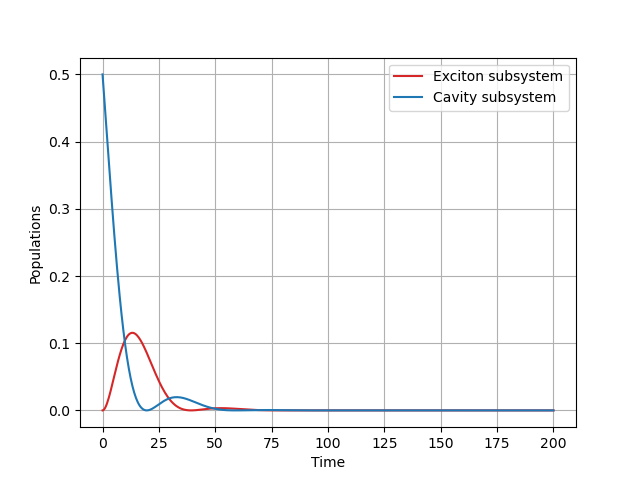
\includegraphics[width=\linewidth]{Research Project/Code/results/JCM/OQS_Pop_Both_eg.png}
        \caption{}
        \label{fig:JCM_OQS_Pop_Both_eg}
    \end{subfigure}
    \hfill

    \caption{Plots of the JCM subsystem populations under open system evolution, with an initial state of $|\psi (\text{t=0})\rangle = 1/\sqrt{2}(|e\rangle + |g\rangle)\otimes|n=0\rangle$. (a) Evolution under spontaneous atomic emission. (b) Evolution under thermal dissipation. (c) Evolution under both spontaneous atomic emission and thermal dissipation.}
    \label{fig:JCM_OQS_Pop_eg}
\end{figure}

\noindent
\\
For coherence, we observe the same features in Figure \ref{fig:JCM_OQS_Coh_eg} as observed with the closed evolution coherence: the $|g,0\rangle$ contribution introduces an off--diagonal term in the full system, creating a baseline level of coherence throughout the evolution, as reflected by the total system's coherence remaining greater than 0. Beyond this, the system's decoherence behaves as expected, with decay timescales matching those of the populations (as also observed for the first initial state), and coherence being present (and thus decaying) in our subsystems. Notably, by starting in an unentangled superposition state, we generate additional coherence in the computational basis, which then decays on a comparable timescale to the populations.\\
\\
Lastly, we observe reduced entanglement in Figure \ref{fig:JCM_OQS_Neg_eg}, arising from the dilution caused by the stationary $|g,0\rangle$ component throughout evolution. Nevertheless, entanglement decays at the same rate as for the previous initial condition, since the initial superposition decays twice as fast, leading to an effectively doubled decay rate for entanglement.\\
\\
This concludes our analysis of the JCM under both closed and open evolution, for two distinct initial states. We now turn to the EVM, to explore how this model may provide novel entanglement and coherence dynamics under both closed and open evolution. 

\begin{figure}[H]
    \centering
    \begin{subfigure}{0.45\textwidth}
        \centering
        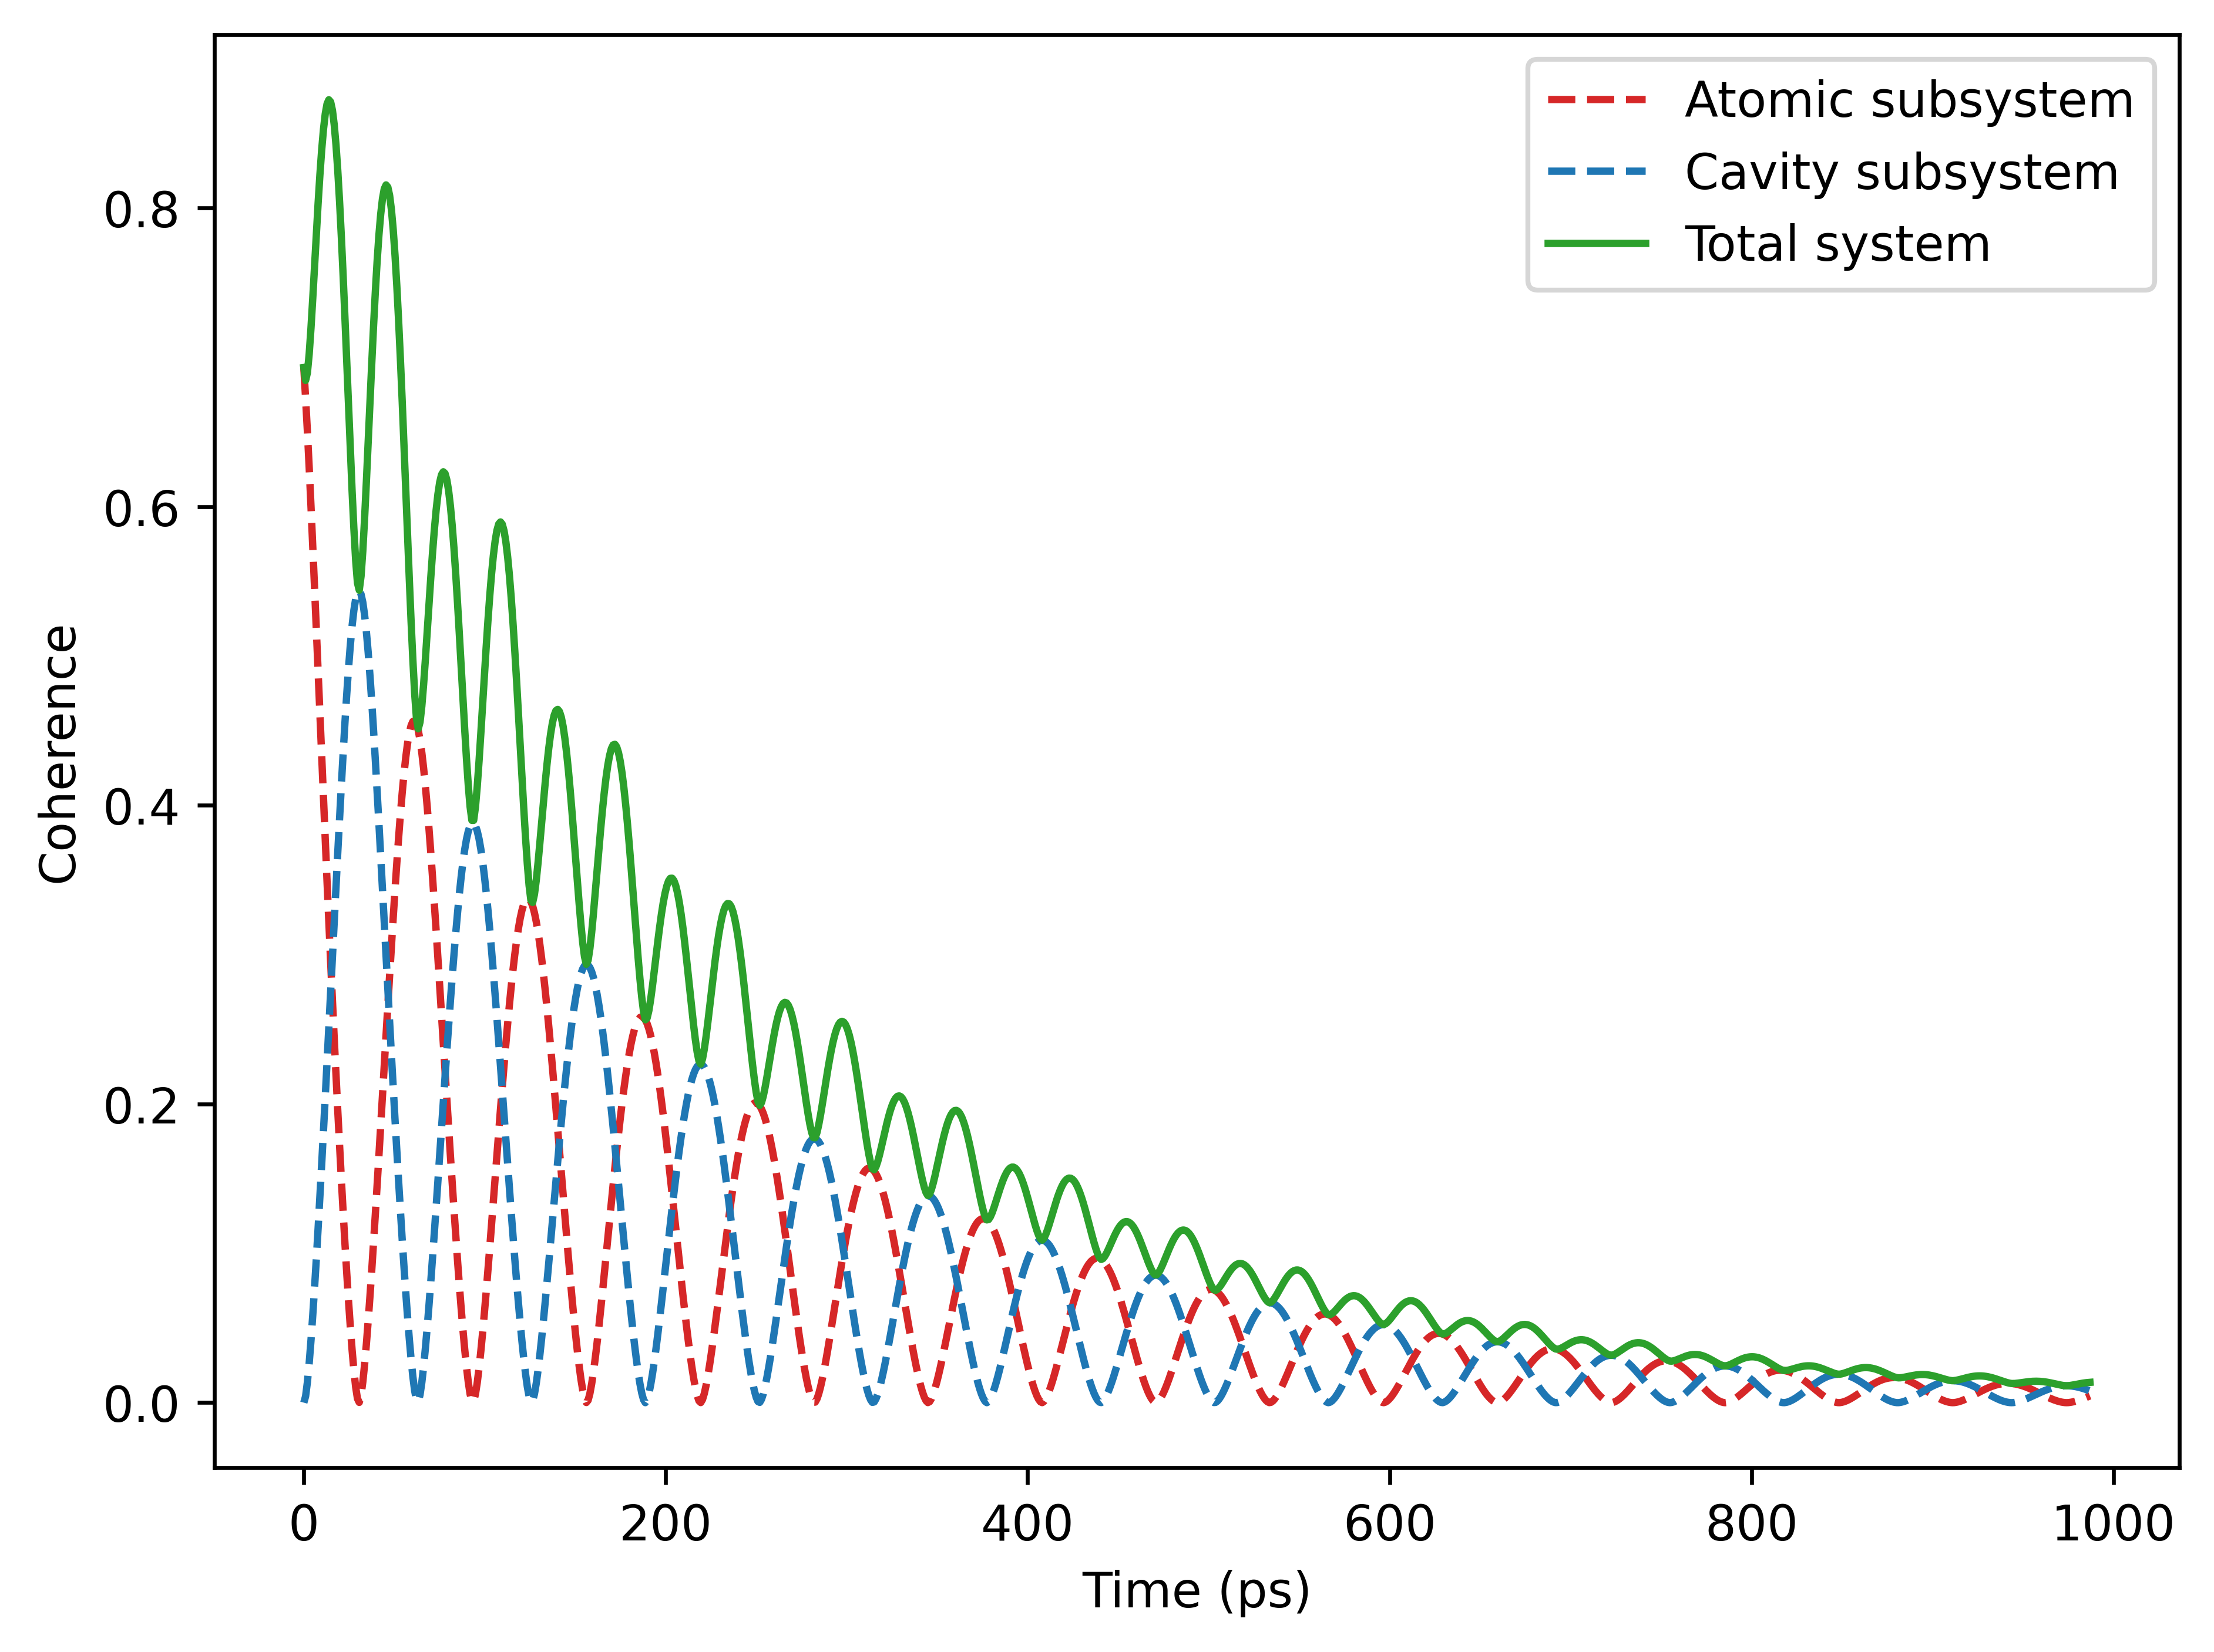
\includegraphics[width=0.85\linewidth]{Research Project/Code/results/JCM/OQS_Coh_Spont_eg.png}
        \caption{}
        \label{fig:JCM_OQS_Coh_Spont_eg}
    \end{subfigure}
    \hfill
    \begin{subfigure}{0.45\textwidth}
        \centering
        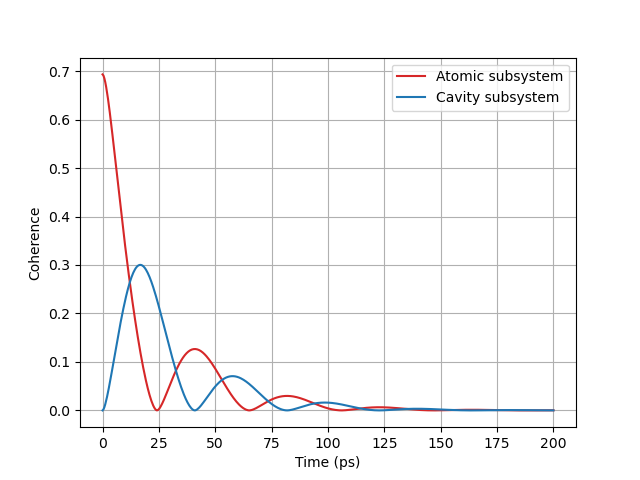
\includegraphics[width=0.85\linewidth]{Research Project/Code/results/JCM/OQS_Coh_Therm_eg.png}
        \caption{}
        \label{fig:JCM_OQS_Coh_Therm_eg}
    \end{subfigure}
    
    \vspace{0.5cm}
    
    \begin{subfigure}{0.45\textwidth}
        \centering
        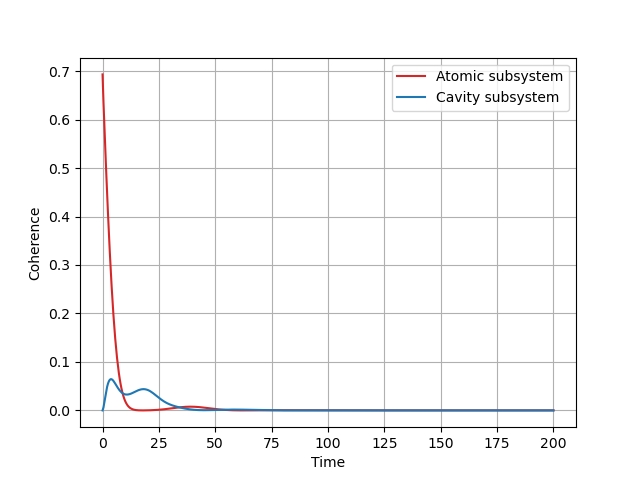
\includegraphics[width=0.85\linewidth]{Research Project/Code/results/JCM/OQS_Coh_Both_eg.png}
        \caption{}
        \label{fig:JCM_OQS_Coh_Both_eg}
    \end{subfigure}
    \hfill
    \caption{Plots of the decay of coherence (decoherence) of the JCM under open system evolution using the relative entropy of coherence measure, with an initial state of $|\psi (\text{t=0})\rangle = 1/\sqrt{2}(|e\rangle + |g\rangle)\otimes|n=0\rangle$. (a) Decoherence under spontaneous atomic emission. (b) Decoherence under thermal dissipation. (c) Decoherence under both spontaneous atomic emission and thermal dissipation.}
    \label{fig:JCM_OQS_Coh_eg}
\end{figure}


\begin{figure}[H]
    \centering
    \begin{subfigure}{0.45\textwidth}
        \centering
        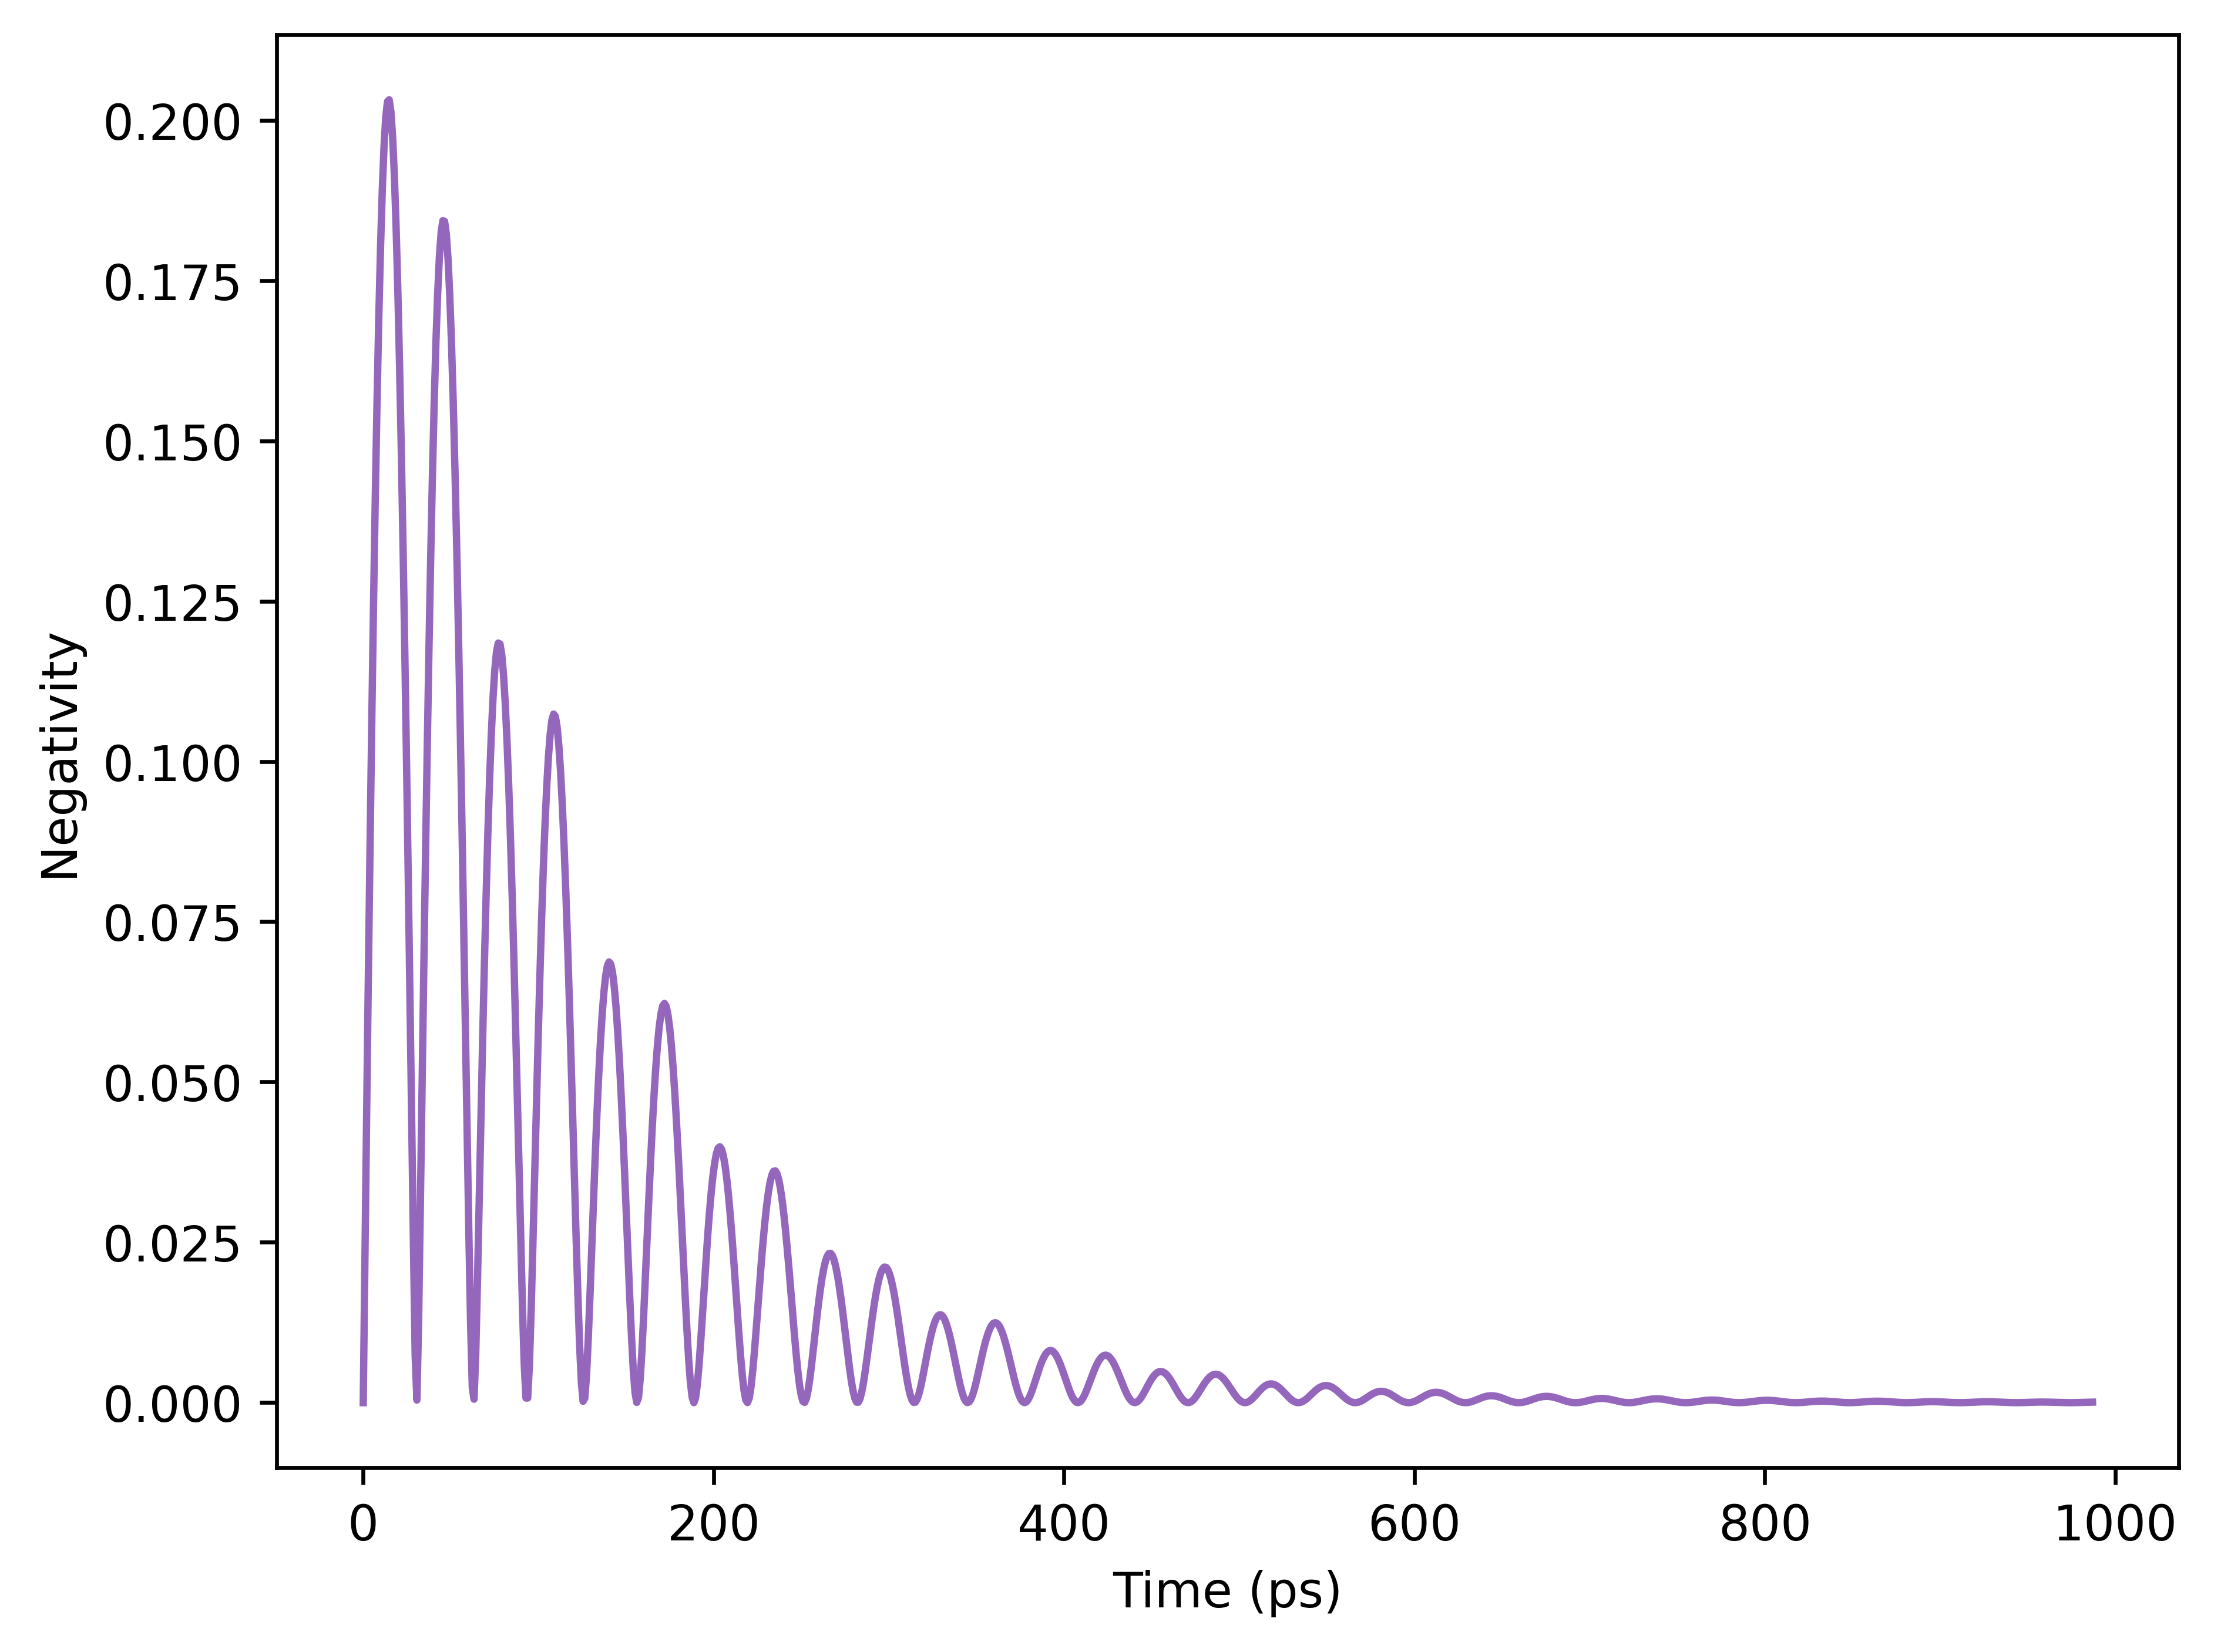
\includegraphics[width=0.85\linewidth]{Research Project/Code/results/JCM/OQS_Neg_Spont_eg.png}
        \caption{}
        \label{fig:jcm_cqs_expt_eg}
    \end{subfigure}
    \hfill
    \begin{subfigure}{0.45\textwidth}
        \centering
        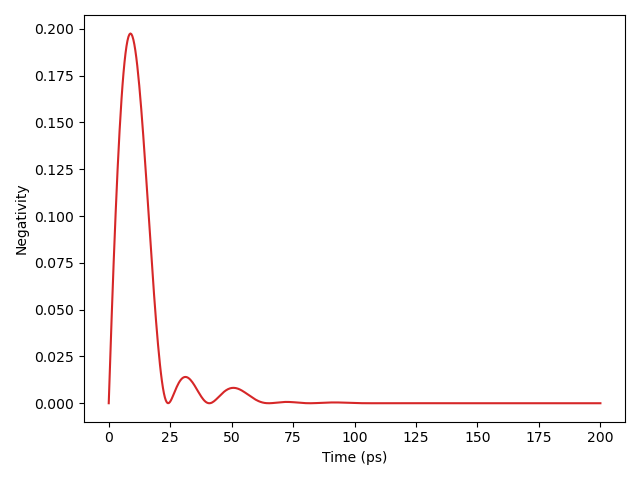
\includegraphics[width=0.85\linewidth]{Research Project/Code/results/JCM/OQS_Neg_Therm_eg.png}
        \caption{}
        \label{fig:jcm_cqs_vne_eg}
    \end{subfigure}
    
    \vspace{0.5cm}
    
    \begin{subfigure}{0.45\textwidth}
        \centering
        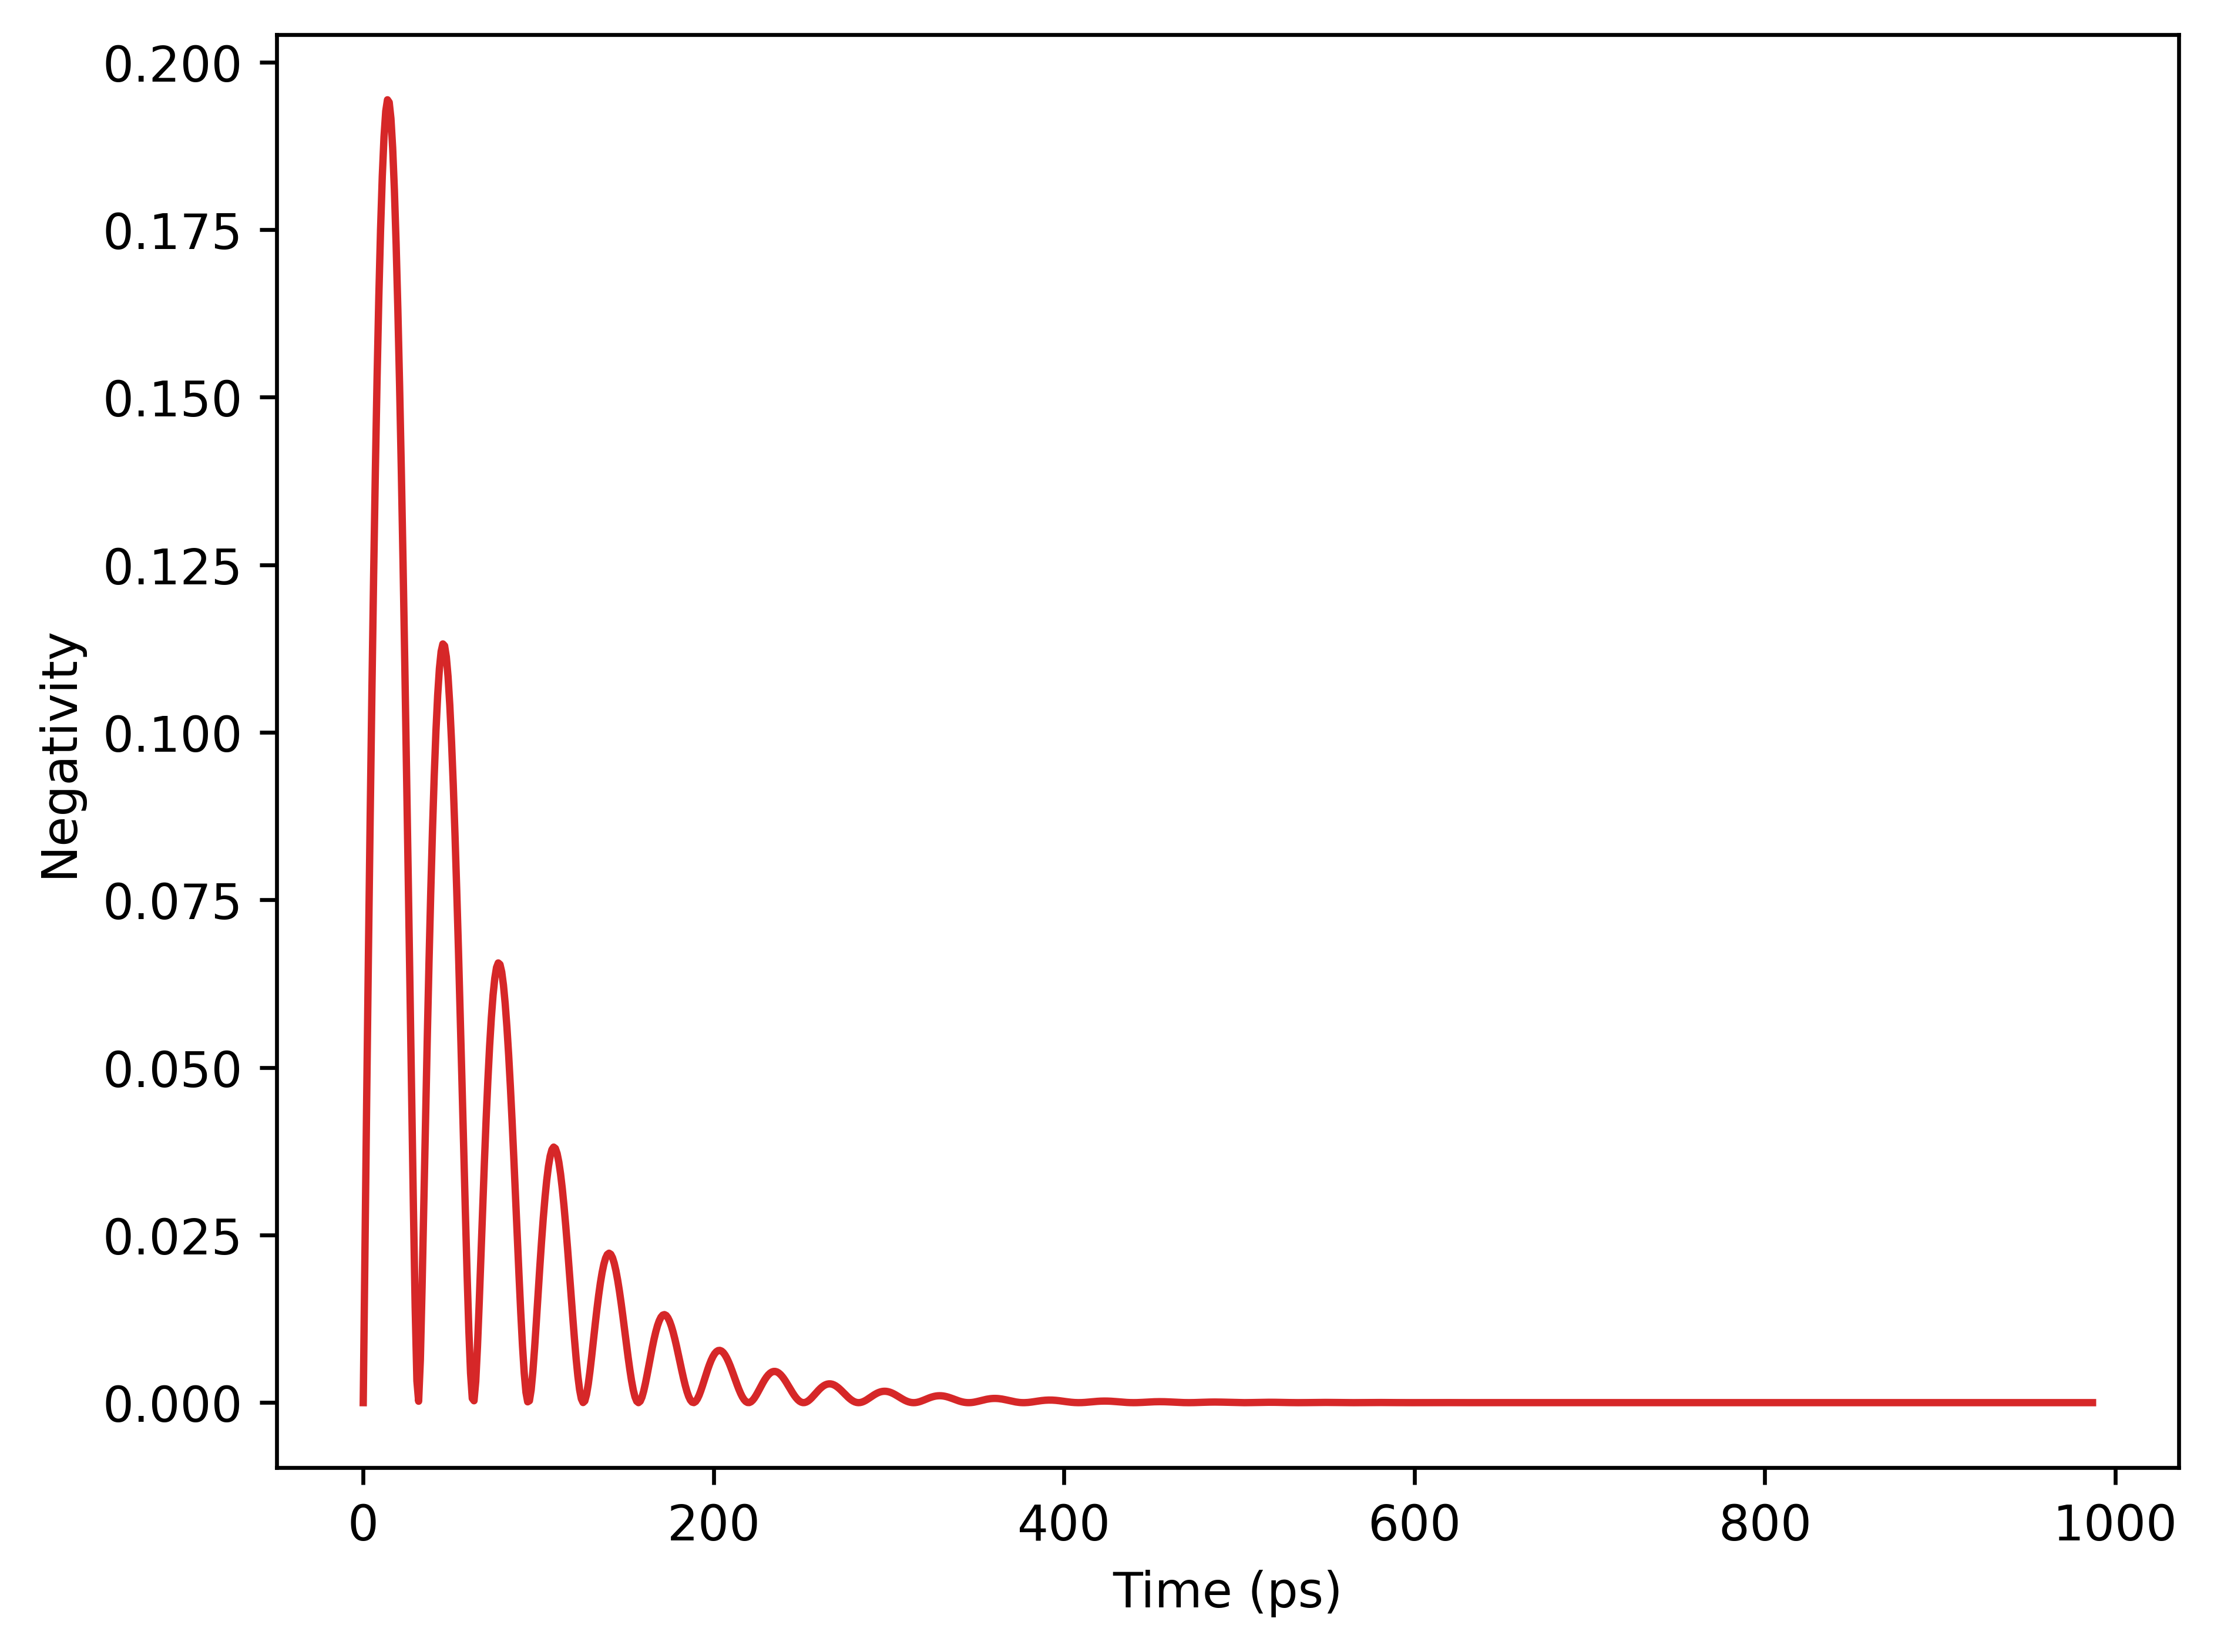
\includegraphics[width=0.85\linewidth]{Research Project/Code/results/JCM/OQS_Neg_Both_eg.png}
        \caption{}
        \label{fig:jcm_cqs_coh_eg}
    \end{subfigure}
    \hfill
    \caption{Plots of the decay of entanglement of the JCM under open system evolution using the negativity measure, with an initial state of $|\psi (\text{t=0})\rangle = 1/\sqrt{2}(|e\rangle + |g\rangle)\otimes|n=0\rangle$. (a) Entanglement decay under spontaneous atomic emission. (b) Entanglement decay under thermal dissipation. (c) Entanglement decay under both spontaneous atomic emission and thermal dissipation.}
    \label{fig:JCM_OQS_Neg_eg}
\end{figure}

%%%%%%%%%%%%%%%%%%%%%%%%%%%%%%%%%%%%%%%%%%%% EVM RESULTS %%%%%%%%%%%%%%%%%%%%%%%%%%%%%%%%%%%
\subsection{Population, Entanglement and Coherence of the Exciton--Vibration Model}

We begin our computational analysis of the EVM by examining subsystem populations, entanglement and coherence under closed (unitary) evolution for two initial conditions. The analysis is then repeated for the same initial conditions within the framework of open quantum dynamics. As outlined in Section \ref{sec:method_sub_EVM}, all plots are smoothed for improved visualisation of trends; this procedure occasionally introduces minor boundary artefacts, seen as small end--point flicks, which have no physical meaning. Furthermore, we present two plots for each result: one showing oscillations on a shorter timescale (left--hand columns), and another on a longer timescale (right--hand columns). Lastly, we retain the raw data, depicted by faint dashed lines, in all plots. 

\subsubsection{Closed Evolution}

\subsubsubsection{Case I: Excited State Initial Condition}

We begin our closed analysis of the EVM by considering the initial state in equation \eqref{eqn:init_EVM_e0}:

\begin{equation*}
    |\psi (\text{t=0})\rangle = |1, 0\rangle.
\end{equation*}


\noindent Figure \ref{fig:EVM_CQS_Pop_e0} illustrates the populations of the effective exciton's excited state and the vibrational mode $|n=0\rangle$. One of the clearest features in the populations is the presence of a hierarchy of oscillations, each traceable to specific energy scales in the Hamiltonian. 

For the exciton subsystem, the fastest oscillations (visible as the faint dashed lines on the right--hand side of the figure) have a period of $\approx0.008$ ps. The Hamiltonian term $\tfrac{\Delta\epsilon}{2}\hat{\sigma}_z$ generates phase evolution; however, in the presence of the exciton--exciton coupling term $V\hat{\sigma}_x$, population transfer is present. Since $\Delta\epsilon \gg V$, the exciton fast oscillations are dominated by $\Delta\epsilon = 1042,\text{cm}^{-1}$. On a slower timescale of $\approx0.1$ ps, we observe medium oscillations that arise from the exciton--vibration coupling $-\tfrac{g}{\sqrt{2}}\hat{\sigma}z(\hat{b}^\dagger+\hat{b})$, which generates coherent exchange between $|1,0\rangle$ and displaced
\begin{figure}[H]
    \centering

    % -------- Row (a): Populations --------
    \begin{subfigure}{\textwidth}
        \centering
        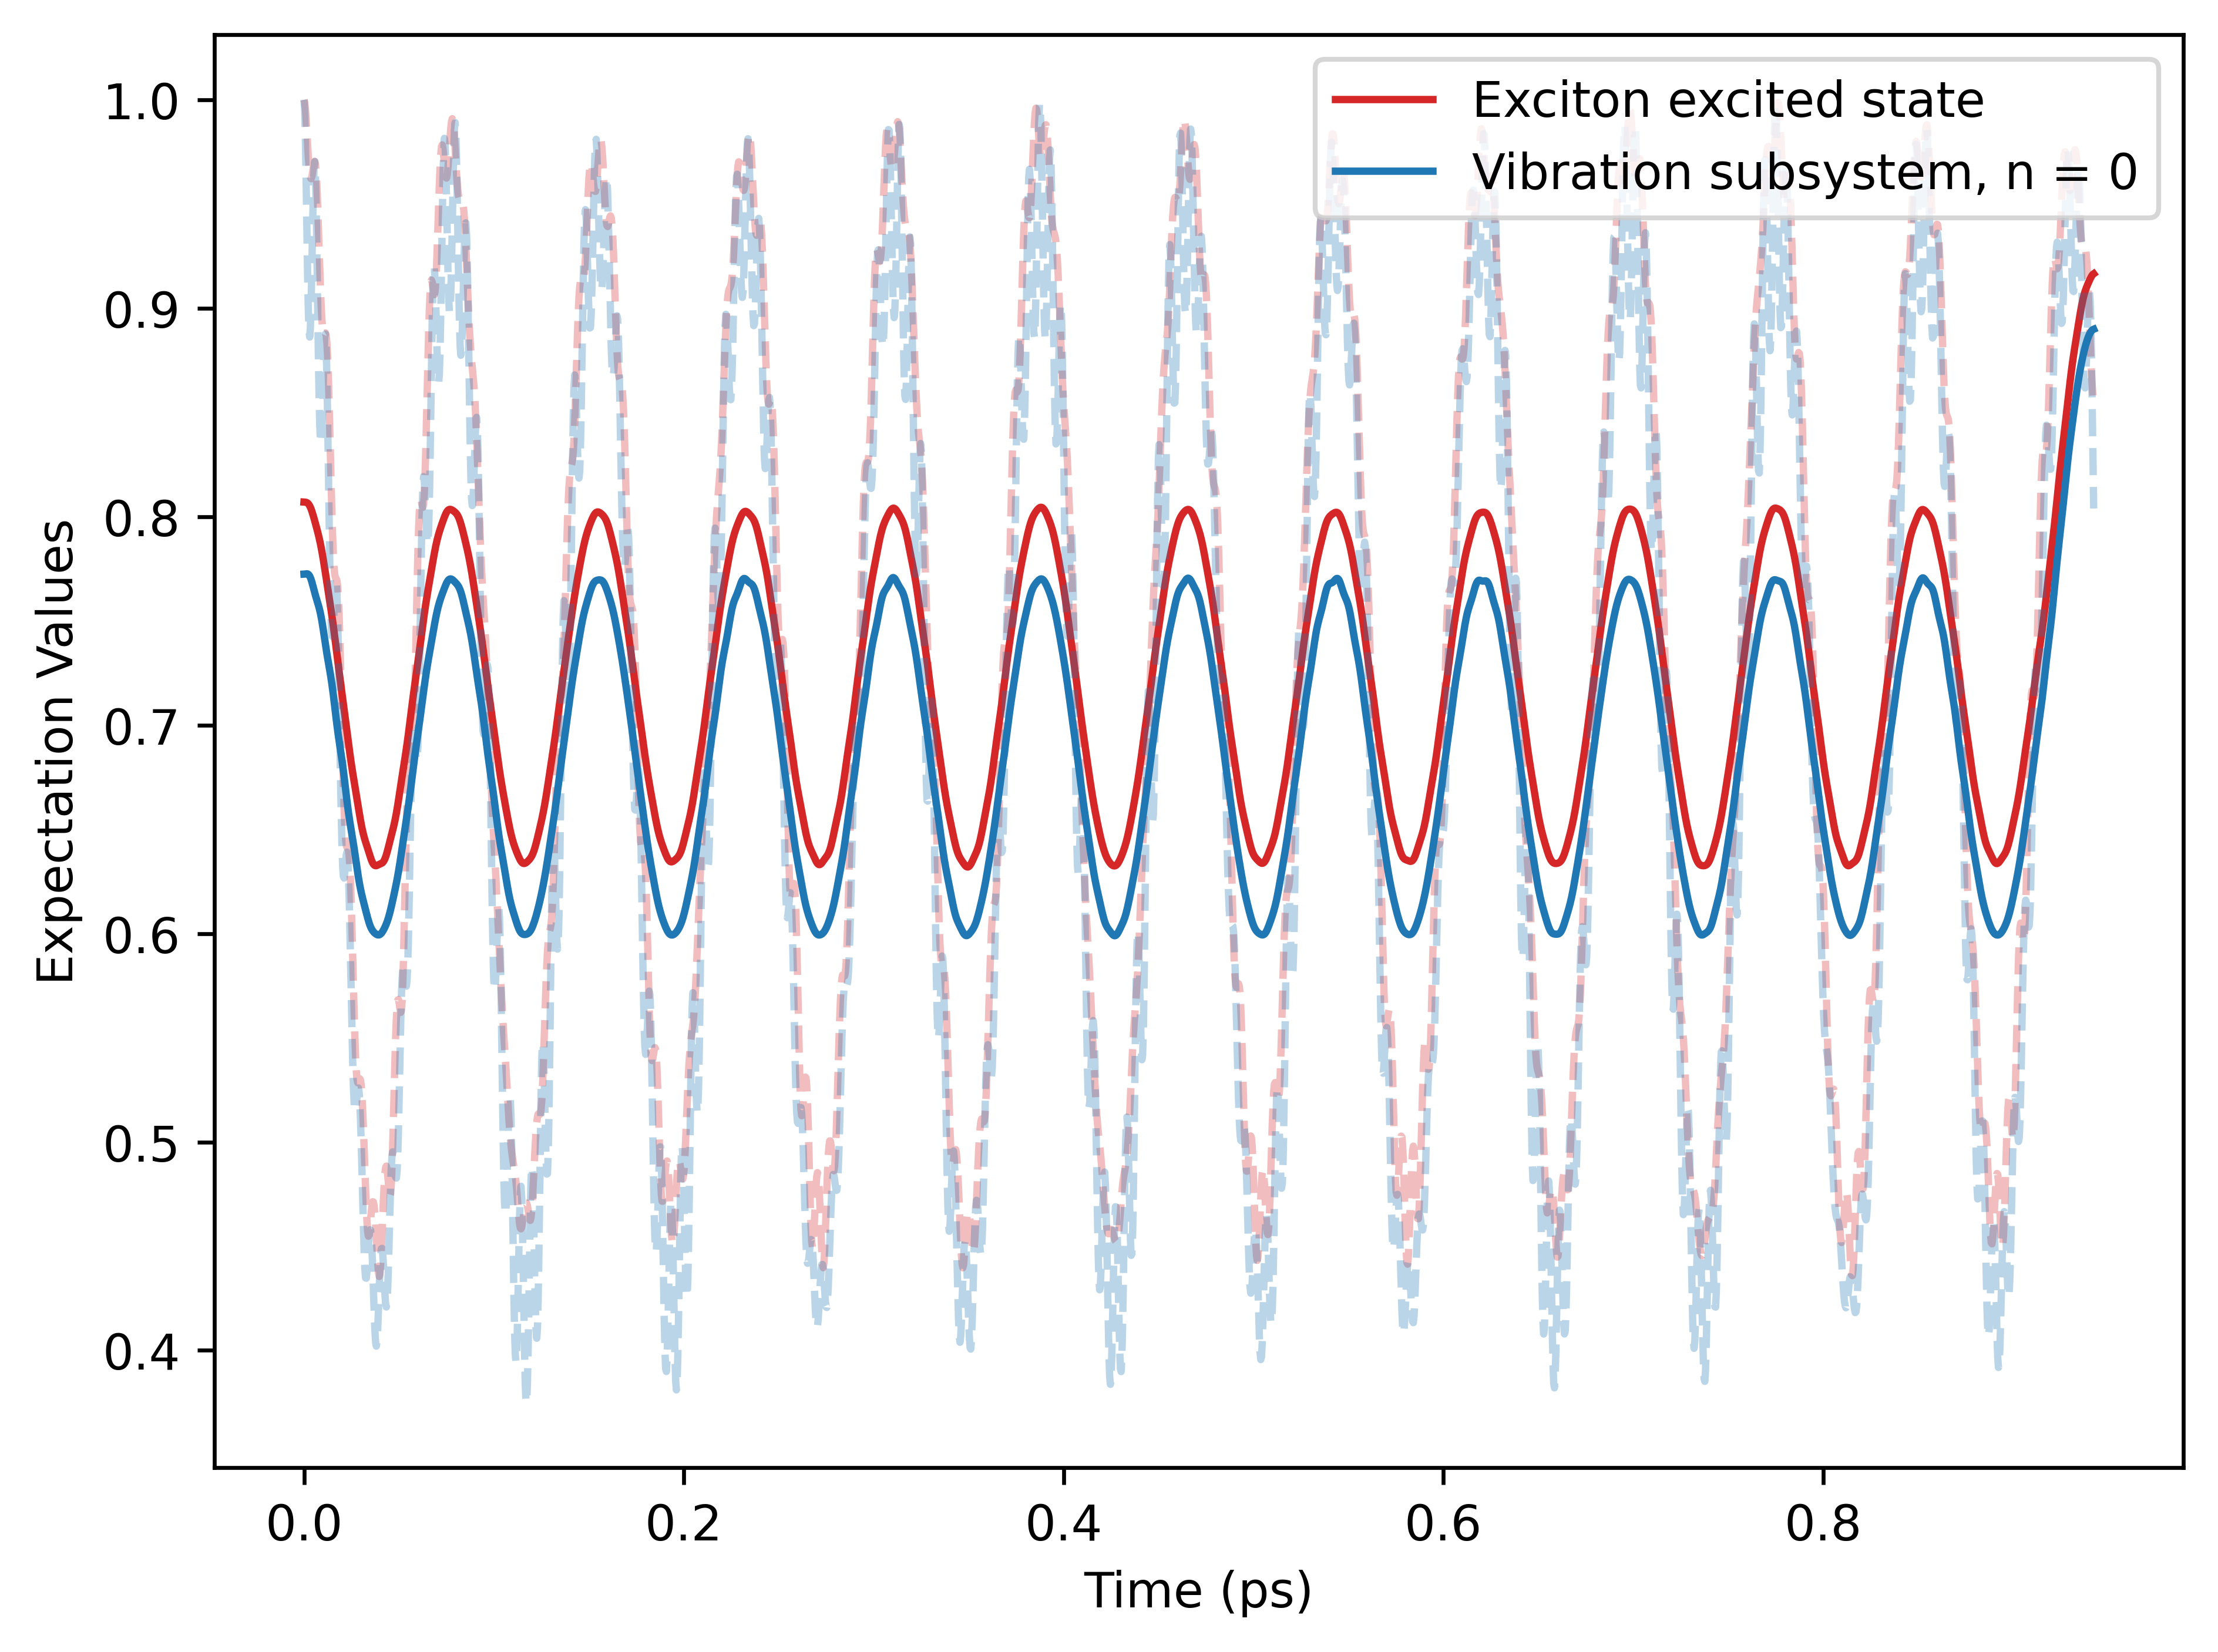
\includegraphics[width=0.49\textwidth]{Research Project/Code/results/ExVib/Closed/Envelope/pops_excited.png}
        \hfill
        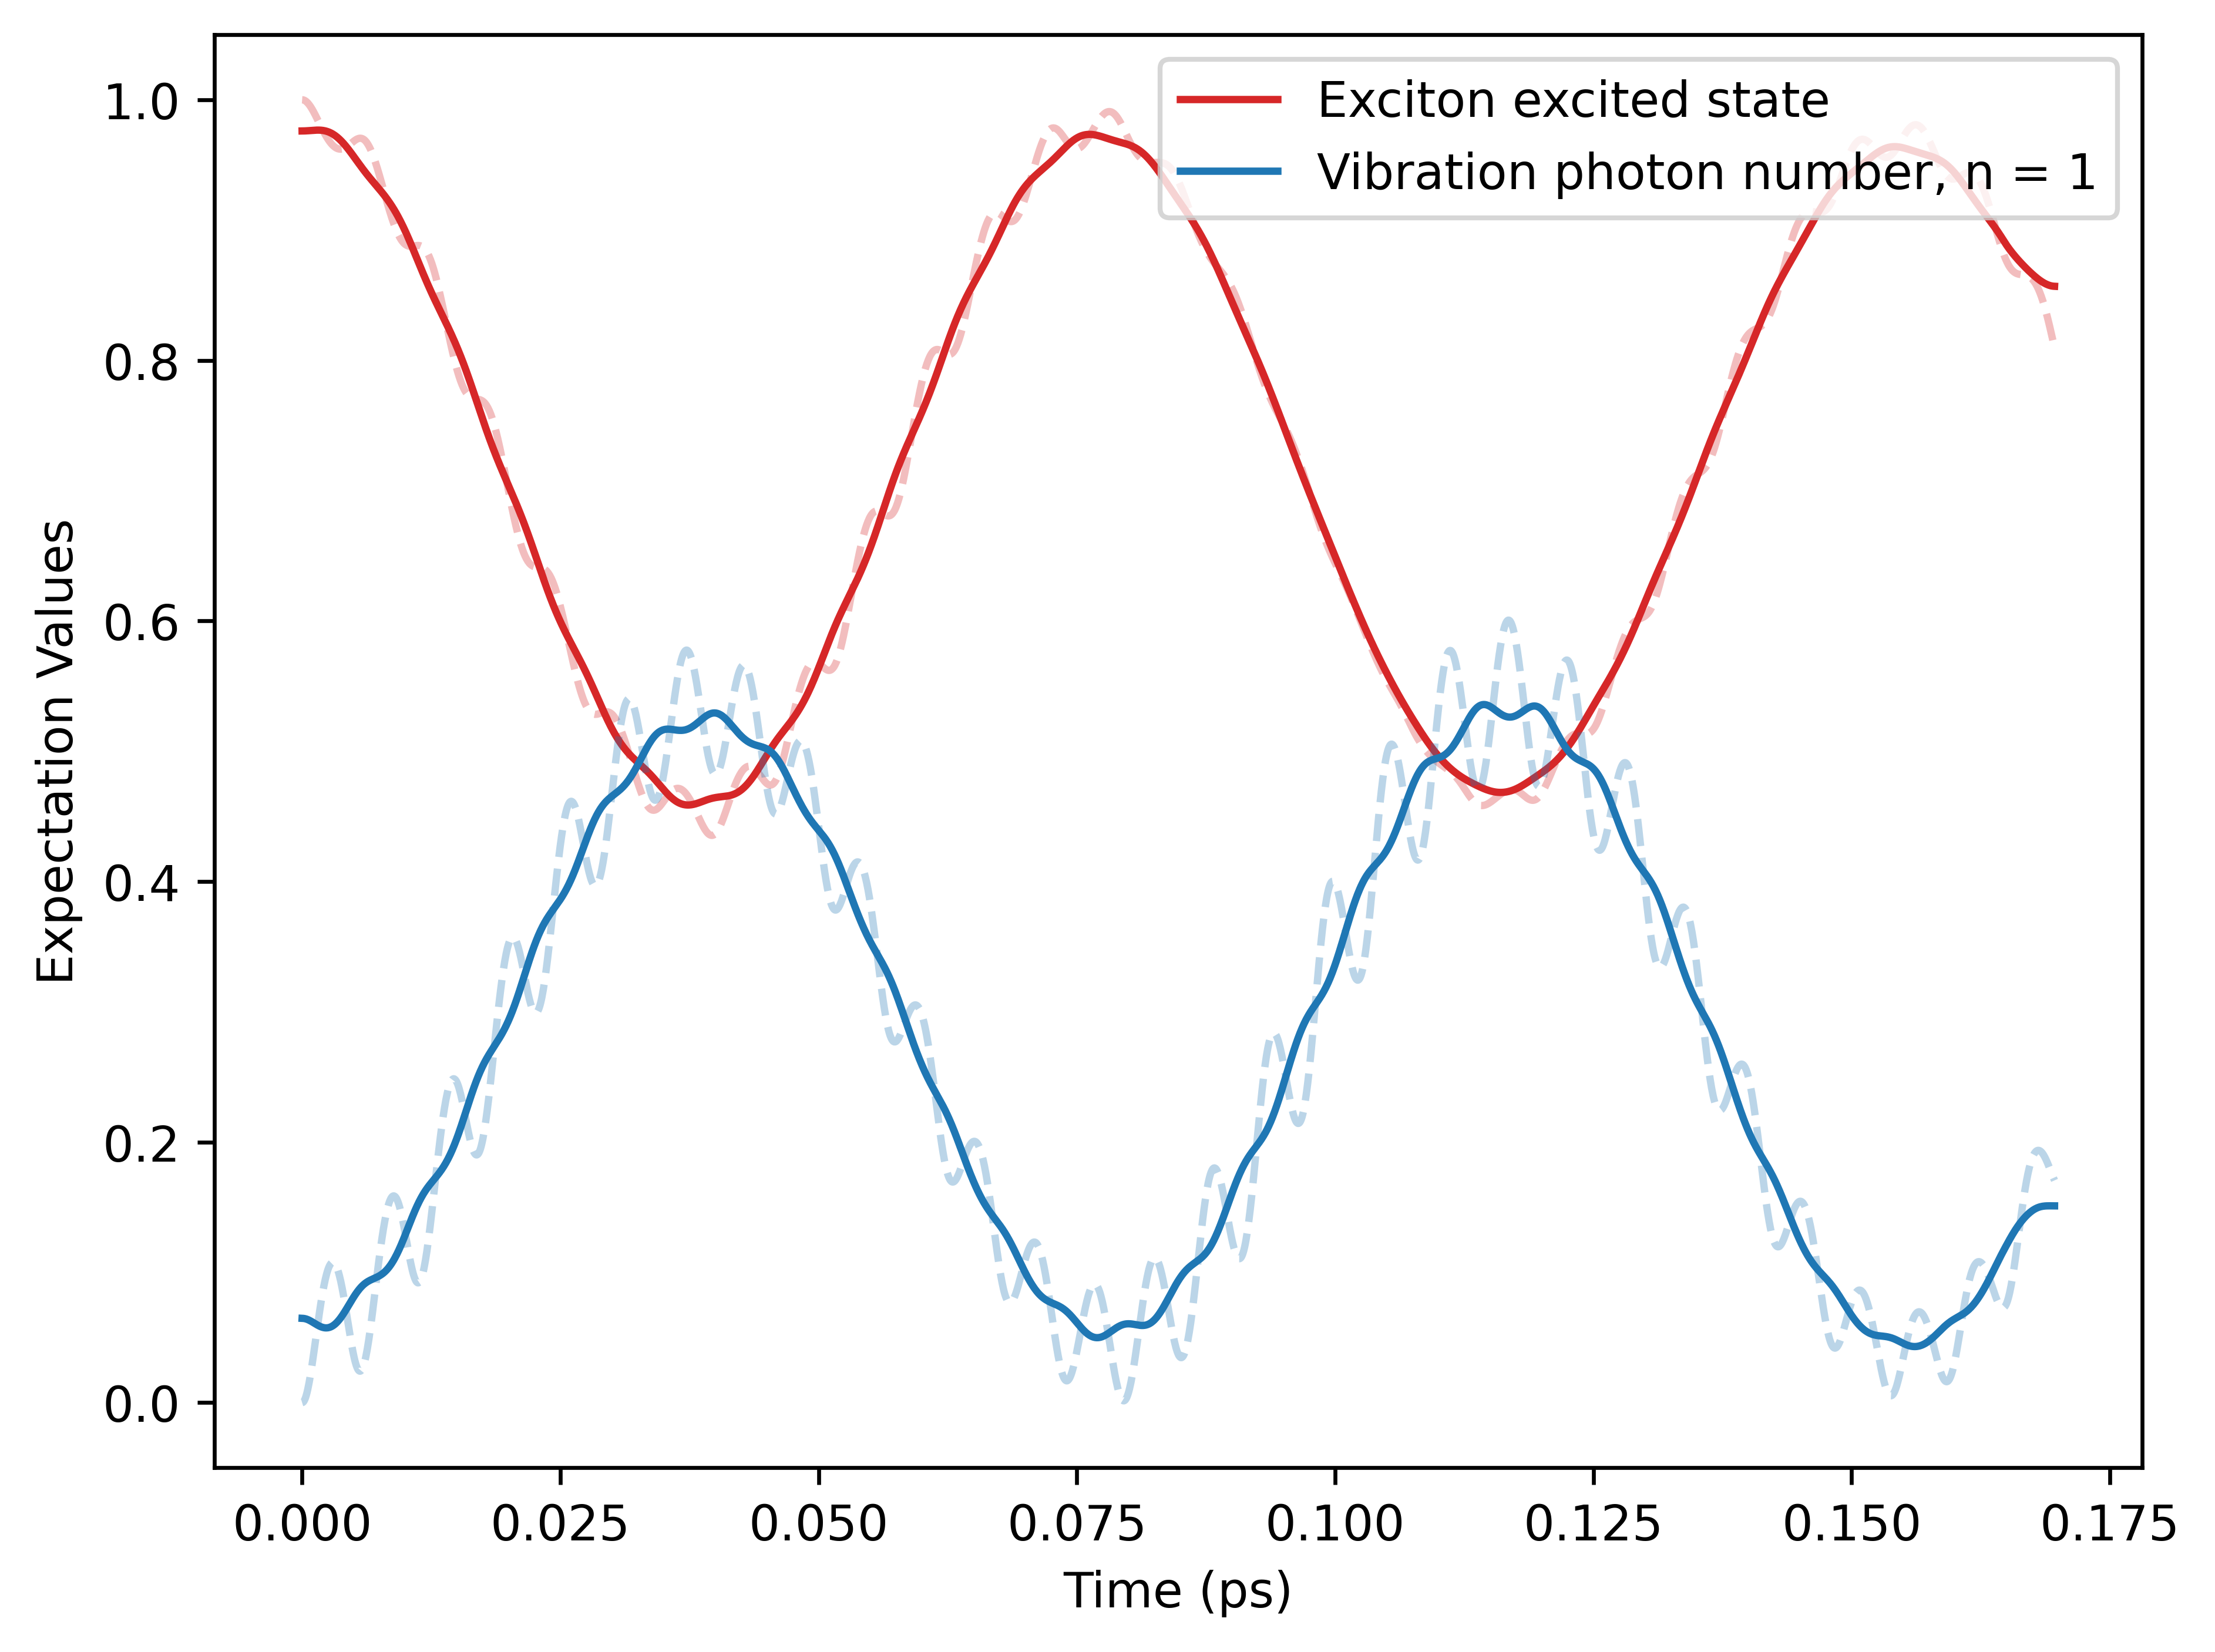
\includegraphics[width=0.49\textwidth]{Research Project/Code/results/ExVib/Closed/Fast/pops_excited.png}
        \caption{}
        \label{fig:EVM_CQS_Pop_e0}
    \end{subfigure}

    \vspace{0.8em}

    % -------- Row (b): Entanglement --------
    \begin{subfigure}{\textwidth}
        \centering
        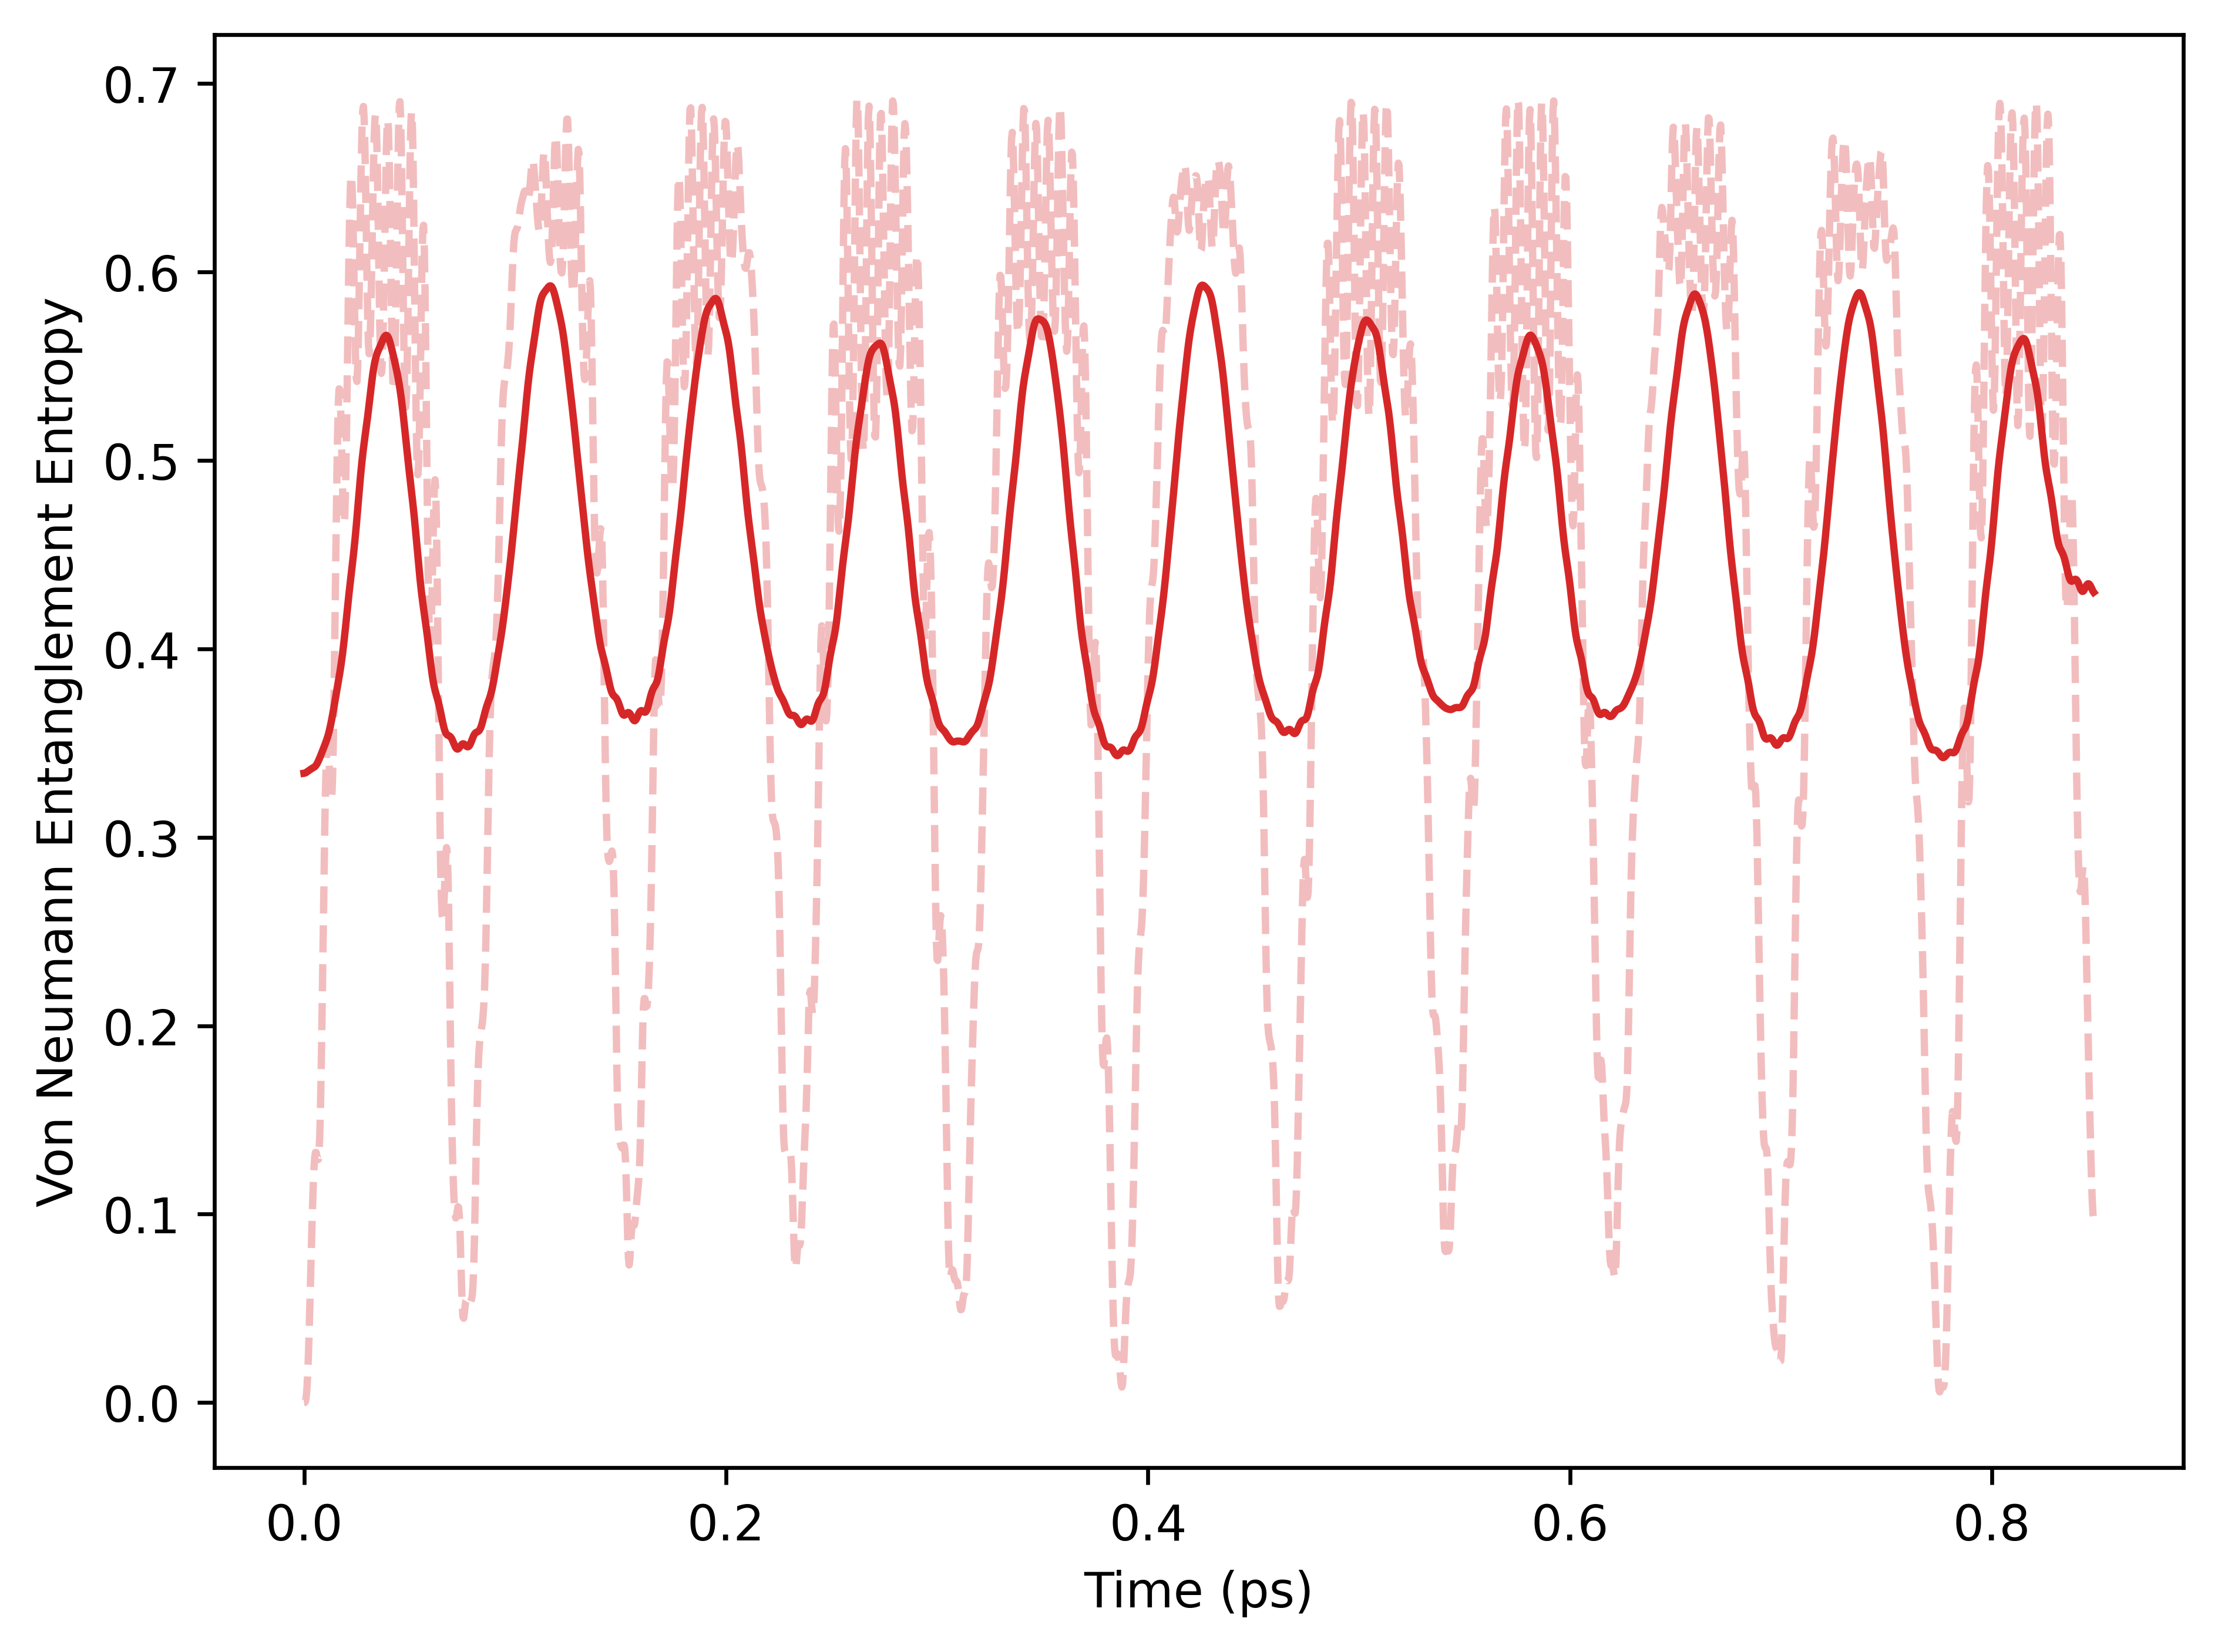
\includegraphics[width=0.49\textwidth]{Research Project/Code/results/ExVib/Closed/Envelope/vne.png}
        \hfill
        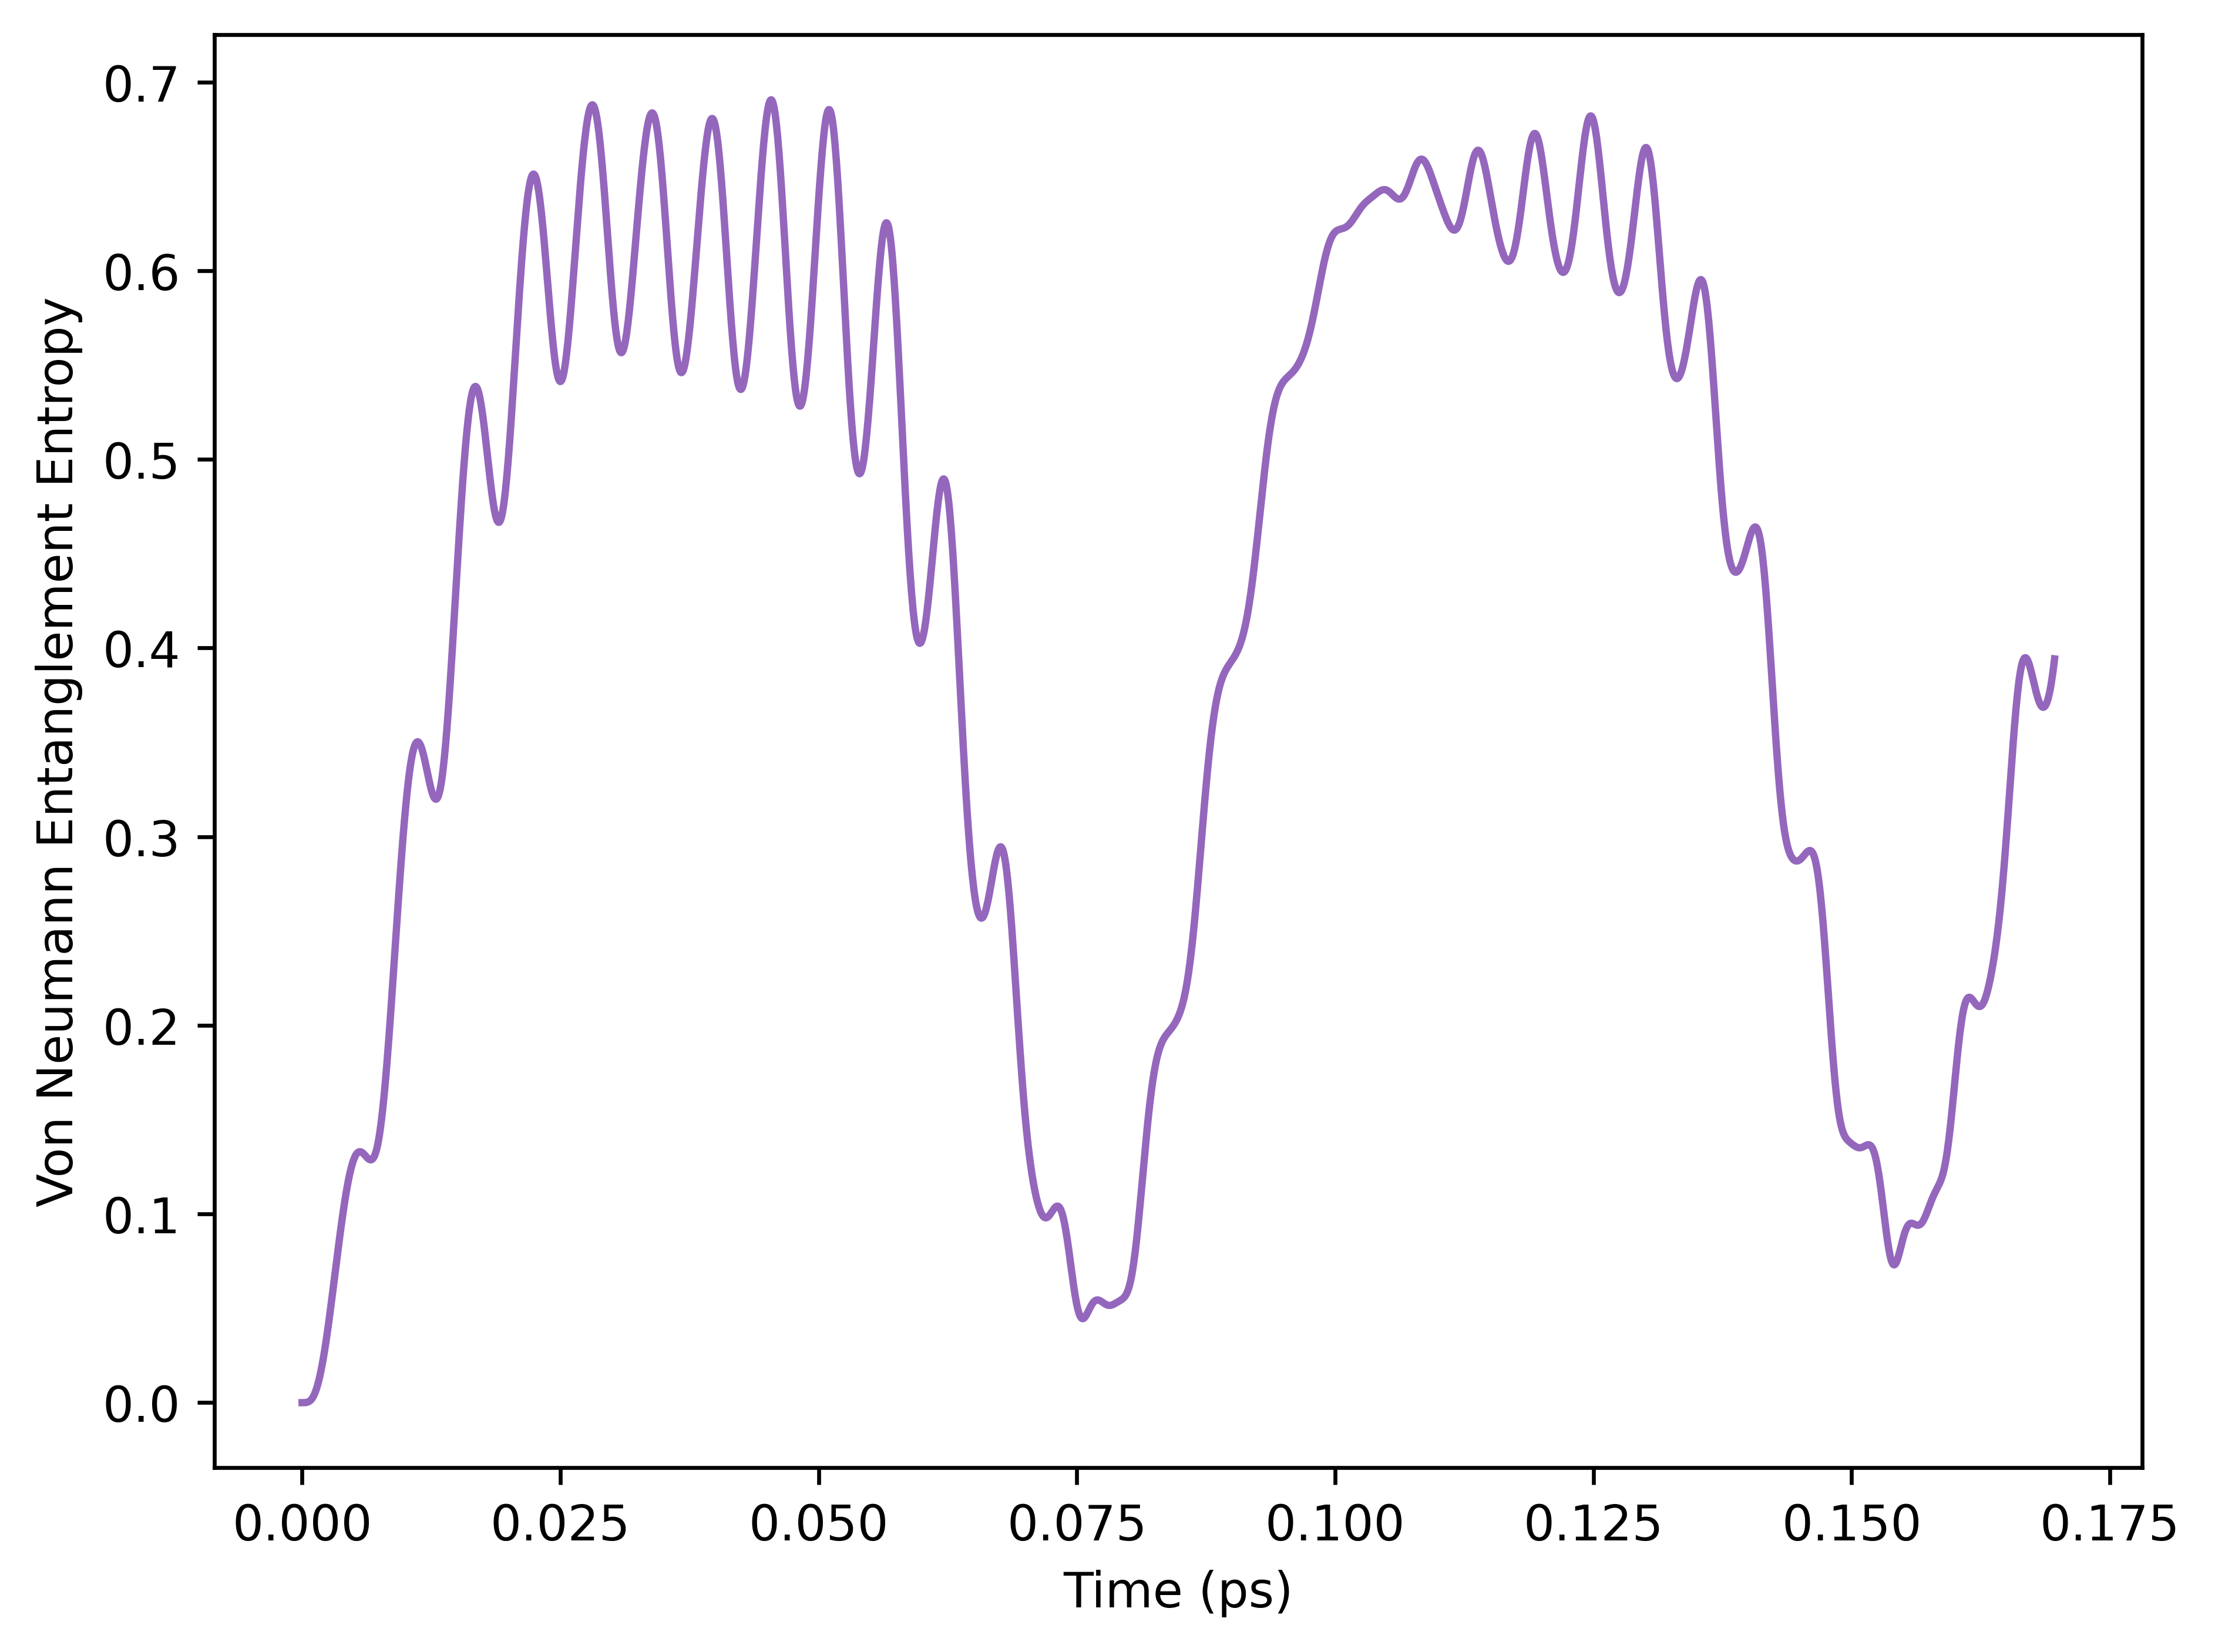
\includegraphics[width=0.49\textwidth]{Research Project/Code/results/ExVib/Closed/Fast/vne.png}
        \caption{}
        \label{fig:EVM_CQS_Ent_e0}
    \end{subfigure}

    \vspace{0.8em}

    % -------- Row (c): Coherence --------
    \begin{subfigure}{\textwidth}
        \centering
        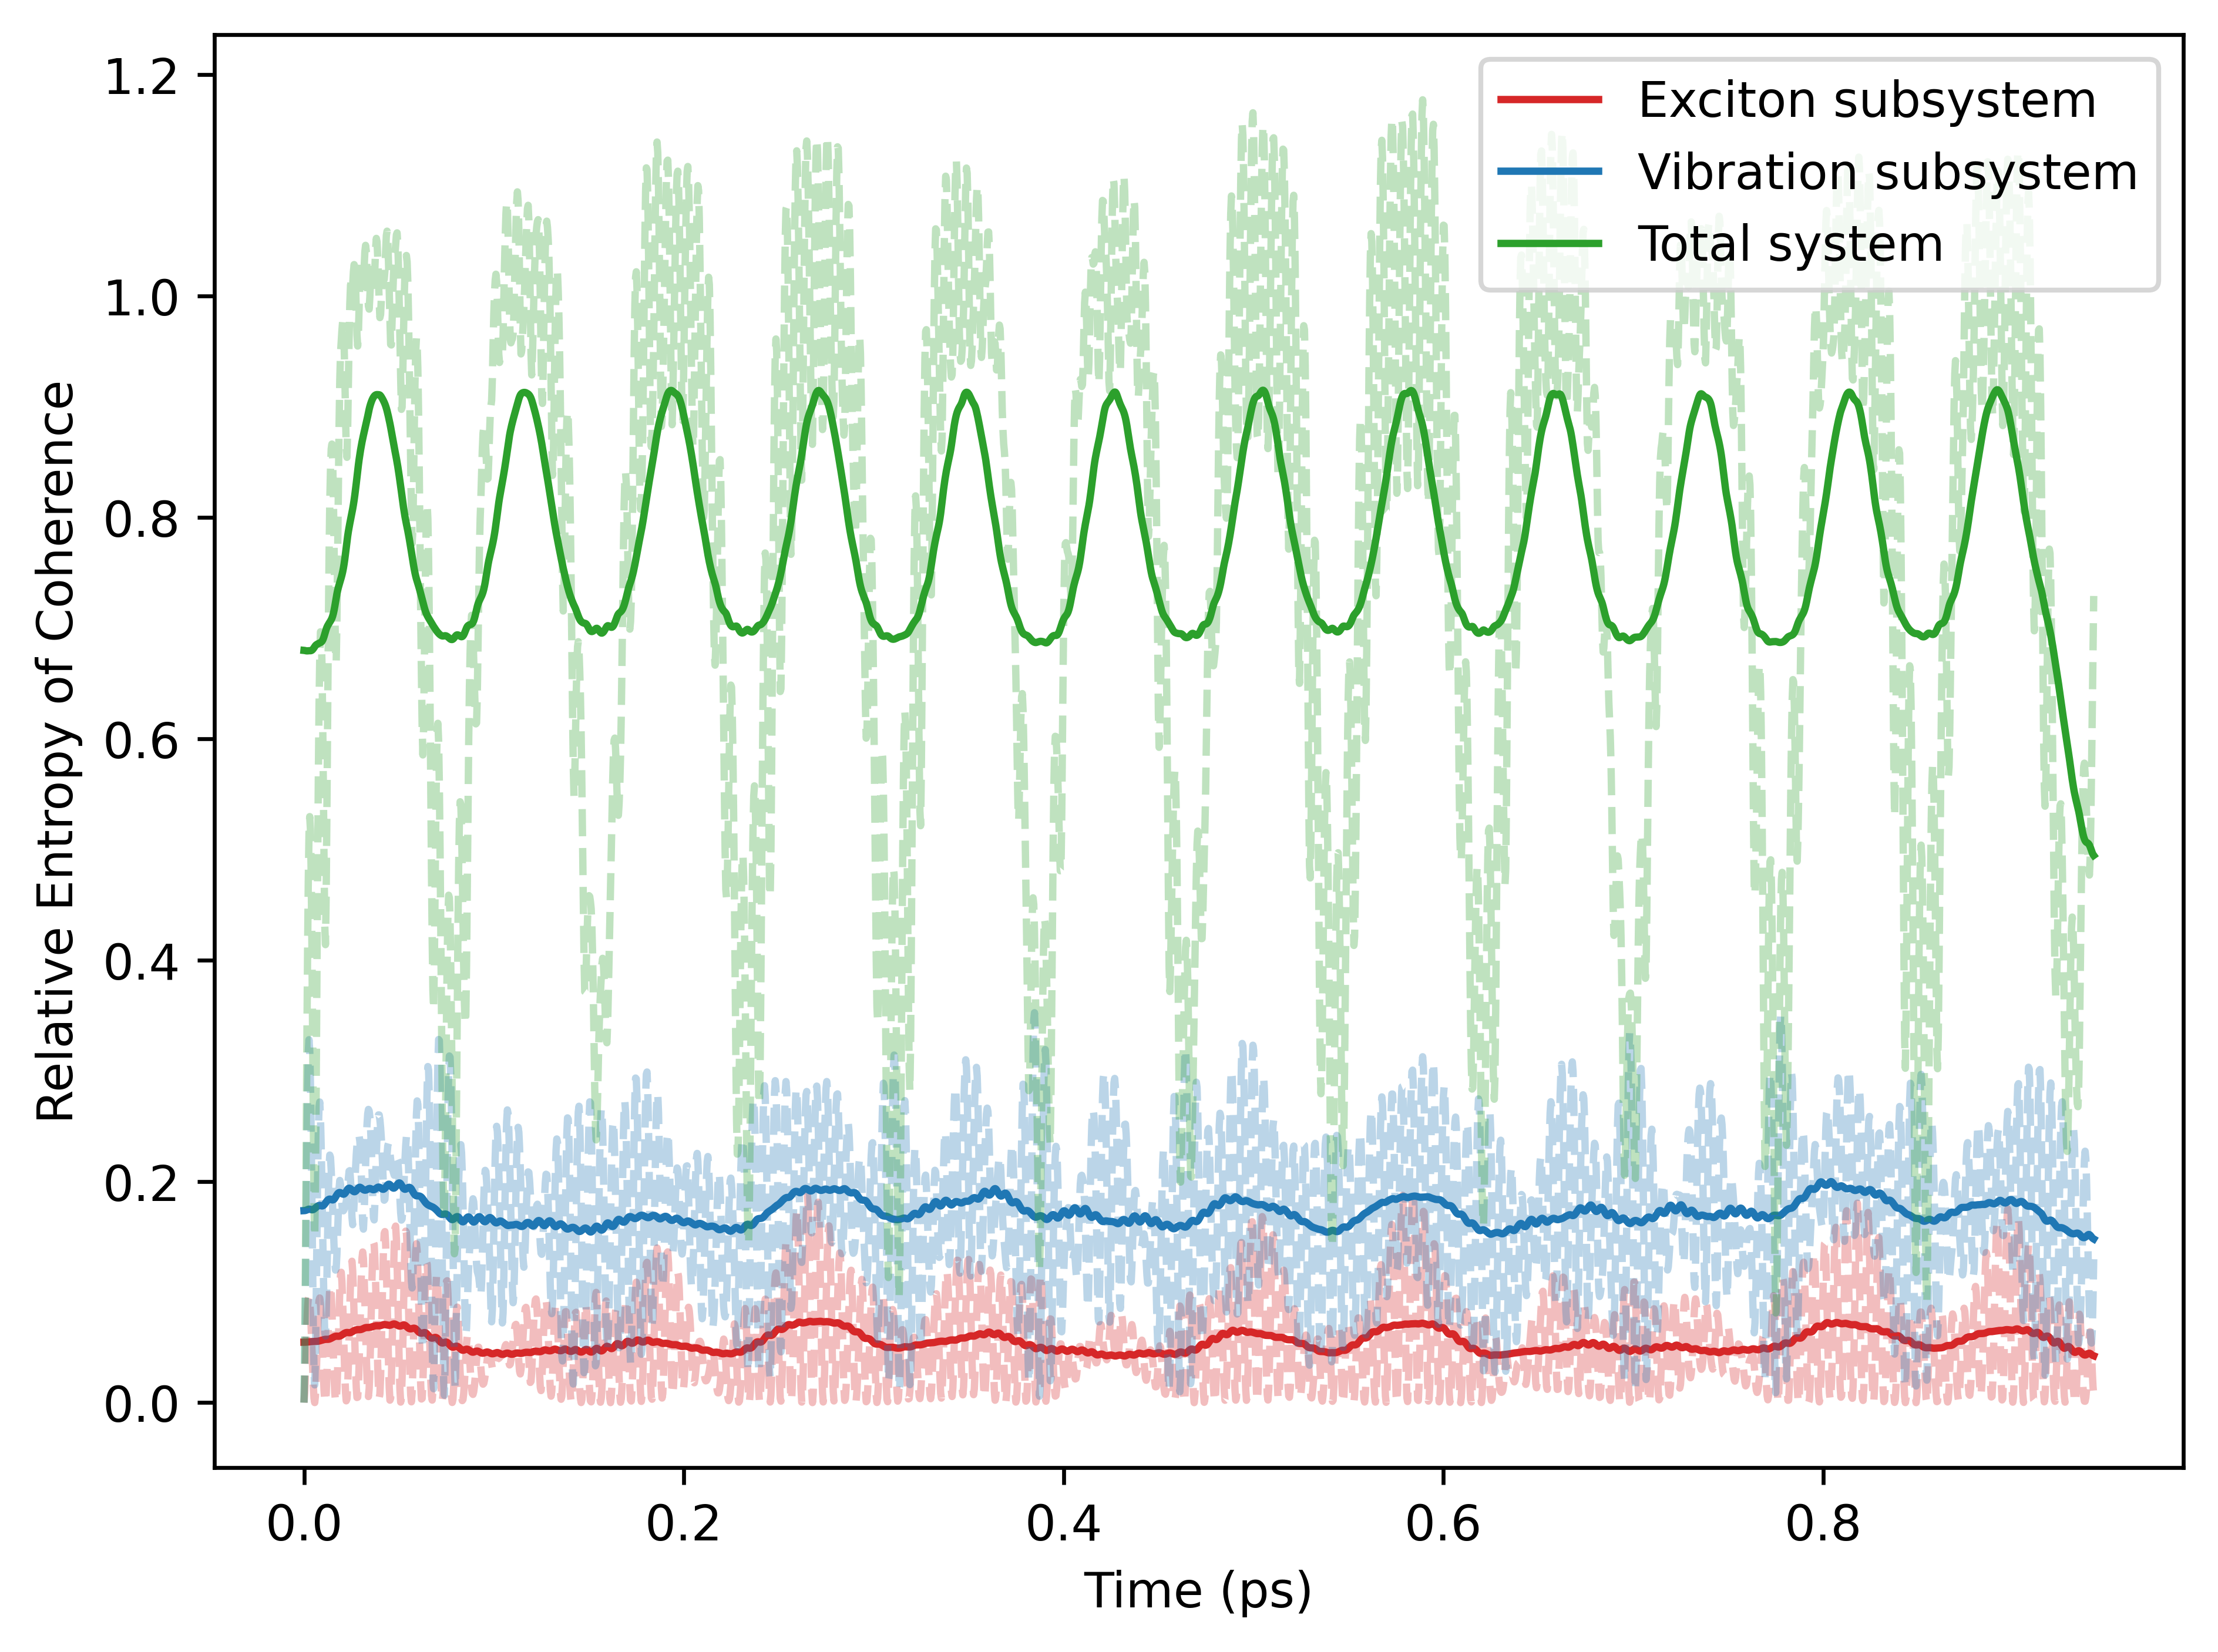
\includegraphics[width=0.49\textwidth]{Research Project/Code/results/ExVib/Closed/Envelope/coh.png}
        \hfill
        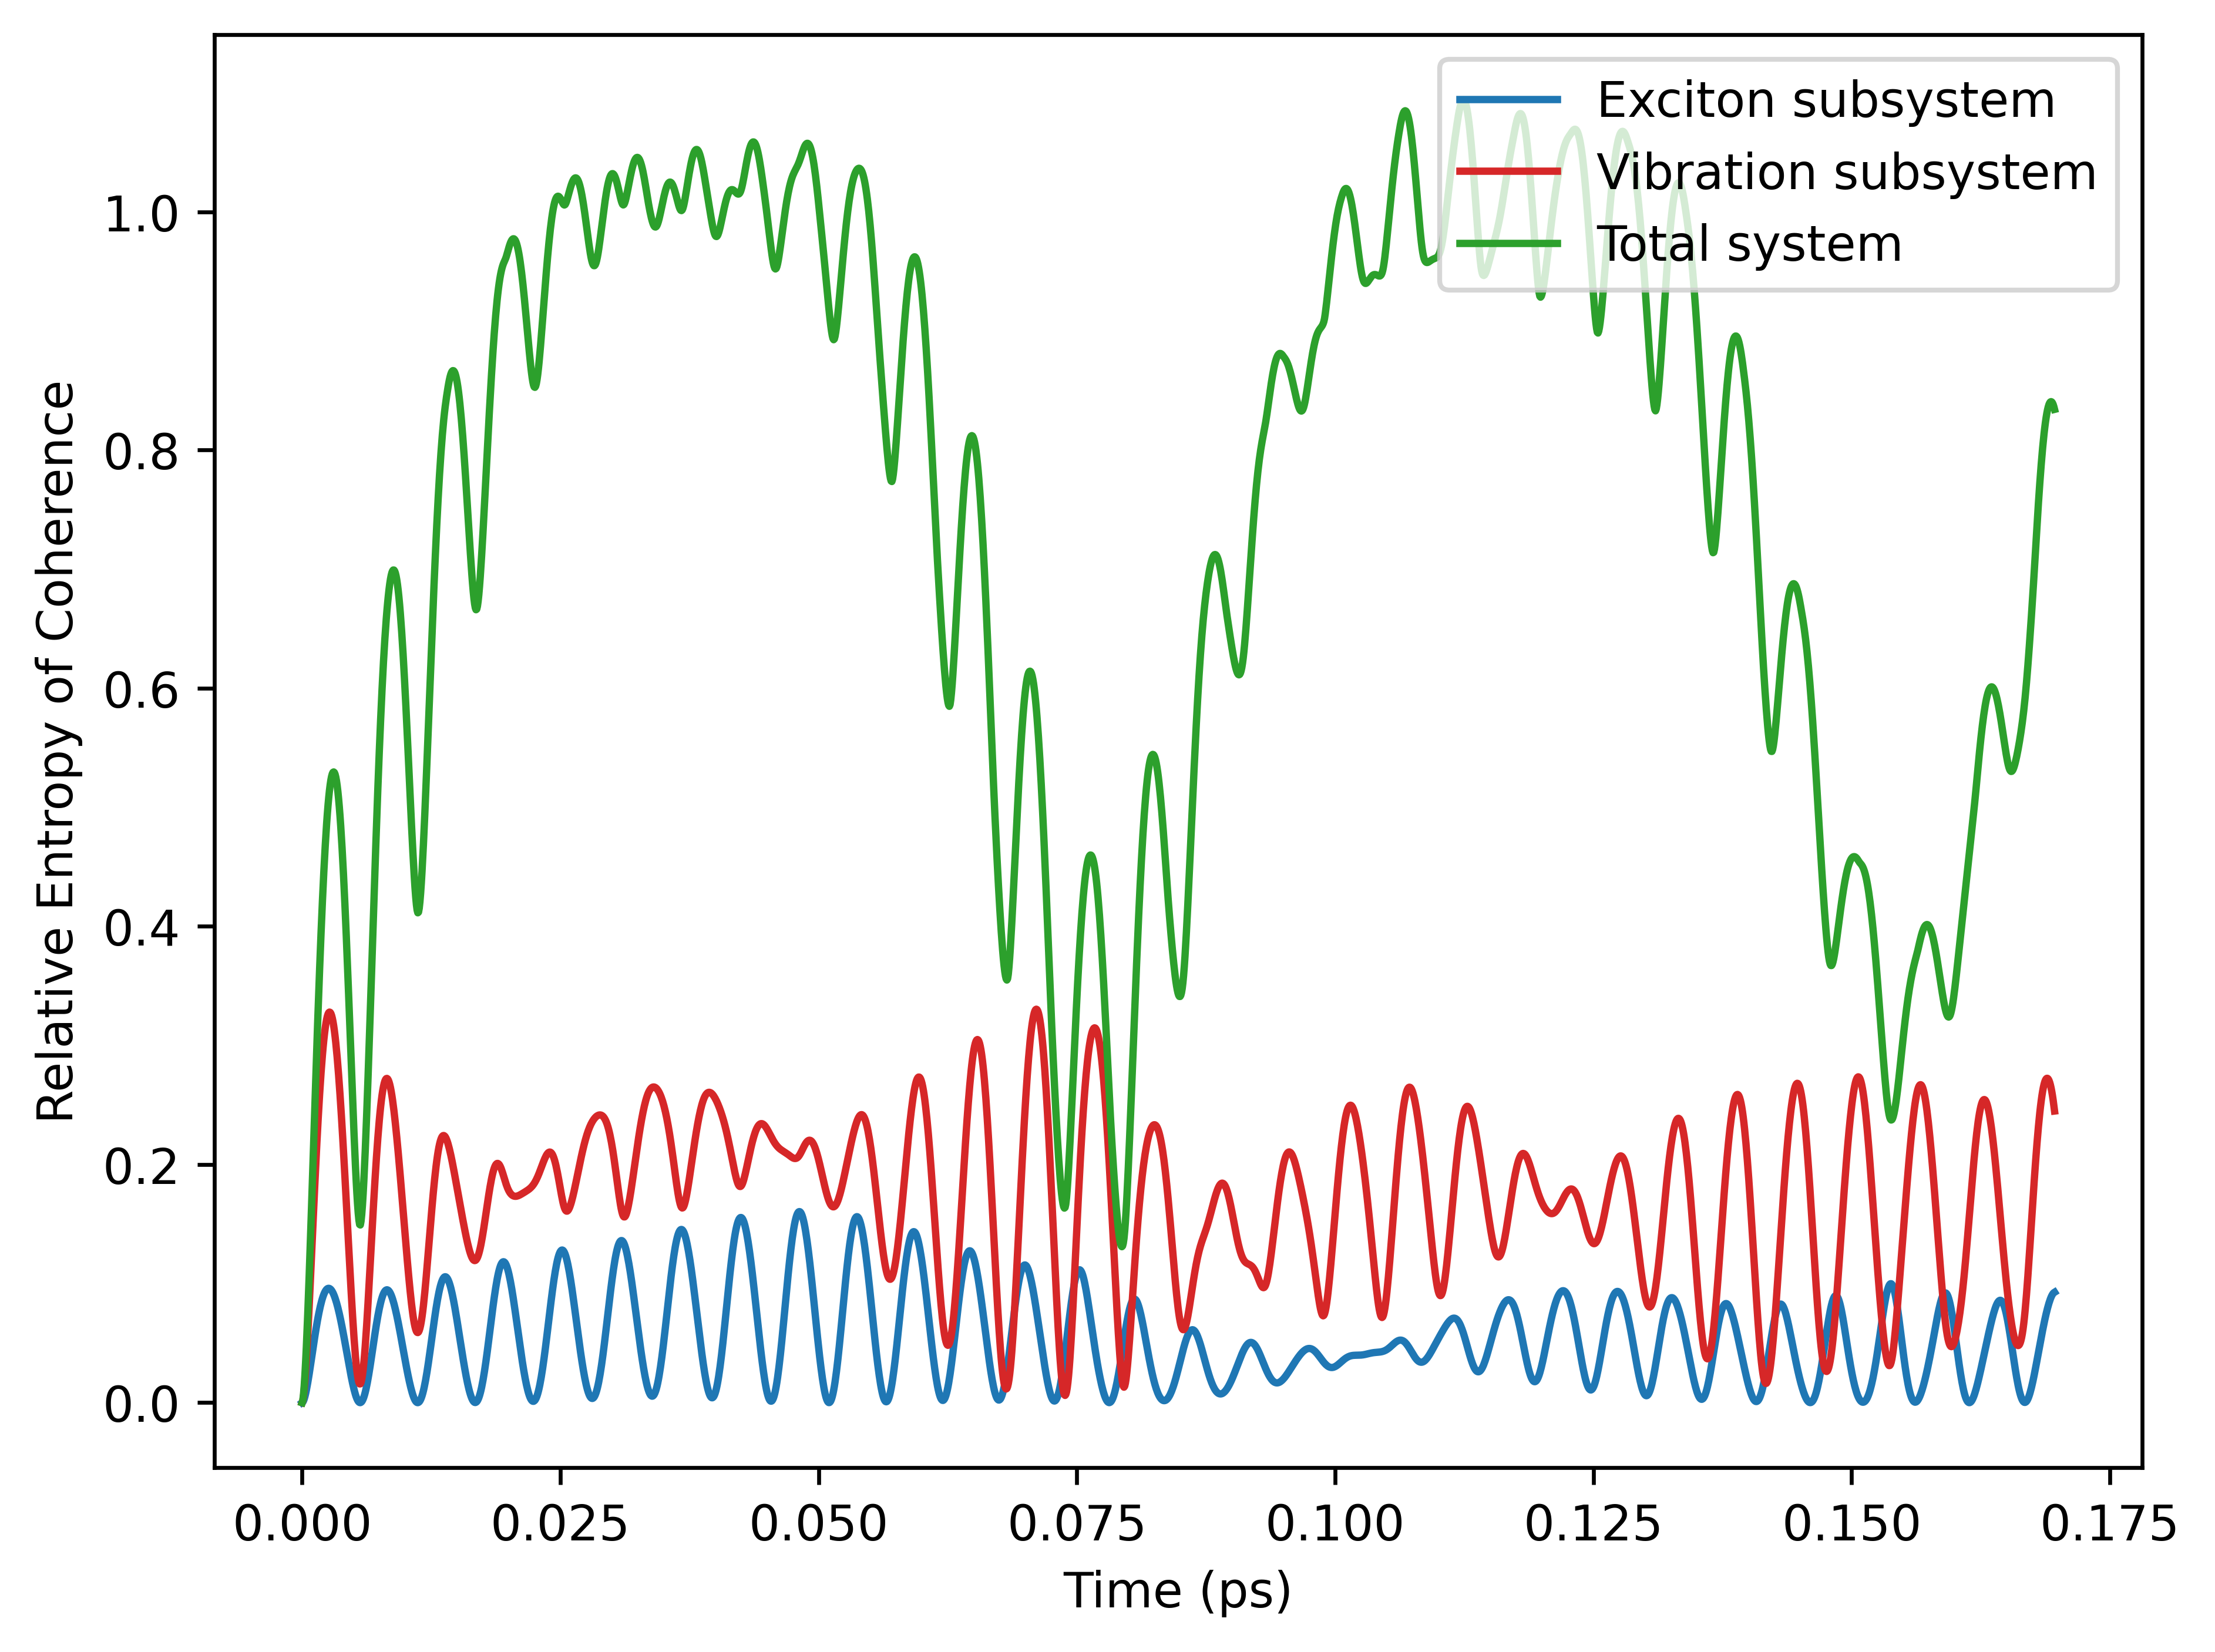
\includegraphics[width=0.49\textwidth]{Research Project/Code/results/ExVib/Closed/Fast/coh.png}
        \caption{}
        \label{fig:EVM_CQS_Coh_e0}
    \end{subfigure}

    \caption{Plots of the EVM under closed unitary evolution with an initial state of $|\psi (\text{t=0})\rangle = |1, 0\rangle$. The left--hand column of sub--figures is plotted over $\approx$ 1 picosecond to demonstrate envelope and medium frequency oscillations. The right--hand column of sub--figures is plotted over a shorter timescale to demonstrate high frequency oscillations. (a) Populations of the excited exciton state $|1\rangle$ and the vibrational mode, $|n=0\rangle$. (b) Entanglement of the total system, quantified by the von Neumann entropy. (c) Coherence of the two subsystems and total system, quantified by the relative entropy of coherence.} 
    \label{fig:EVM_CQS_e0}
\end{figure}

\noindent vibrational states. Finally, the exciton population displays a slow envelope with a period of $\approx0.7$–$0.8$ ps, produced by the small detuning $|\Delta\epsilon - \omega{\scriptscriptstyle \text{vib}}| = 53,\text{cm}^{-1}$, which gives rise to an overall beating modulation.

For the vibrational subsystem, the fastest oscillations have a period of $\approx0.006$ ps. These reflect the bare vibrational frequency $\omega_{\scriptscriptstyle \text{vib}} = 1111,\text{cm}^{-1}$. Unlike the exciton subsystem, population transfer here is generated by the exciton--vibration interaction $\omega_{\scriptscriptstyle \text{vib}} \hat{b}_{\scriptscriptstyle \text{rd}}^\dagger \hat{b}_{\scriptscriptstyle \text{rd}}$ with $\omega_{\scriptscriptstyle \text{vib}}$ being dominant due to $\omega_{\scriptscriptstyle \text{vib}}\gg g$. The same medium oscillations of $\approx0.1$ ps are also present, again set by the coupling $g = 267.1,\text{cm}^{-1}$, and matching those of the exciton subsystem. Finally, the vibrational ground–state population exhibits the same slow envelope with of $\approx0.7$–$0.8$ ps, consistent with the beat frequency generated by the near--resonance between the exciton splitting and the vibrational mode.

Another interesting feature is that the initial condition never vanishes (at no points is the population 0 for either subsystem in Figure \ref{fig:EVM_CQS_Pop_e0}). The terms $\frac{\Delta\epsilon}{2}\sigma_z\text{ and } \omega_{\scriptscriptstyle \text{vib}}\hat{b}_{\scriptscriptstyle \text{rd}}^\dagger\hat{b}_{\scriptscriptstyle \text{rd}}$ are diagonal in their own bases, and therefore always maintain a non--zero contribution from the original exciton and vibrational states.\\
\\
For entanglement, we observe the fast, medium and envelope oscillations in Figure \ref{fig:EVM_CQS_Ent_e0}. It follows the same medium oscillation and envelope frequency beating as with the populations. The fast oscillations, however, correspond to both bare frequencies $\Delta\epsilon$ and $\omega_{\scriptscriptstyle \text{vib}}$, since entanglement reflects the dynamics of the total system. At time $t = 0$, no entanglement is present because the initial state is a product state. Entanglement first reaches its maximum at $t \approx 0.05$ ps with a value of $\ln 2$. This is expected, since for pure states such as our initial state, the von Neumann entropy of either subsystem is equal; the exciton is modelled as an effective TLS, whose maximum entropy is $\ln 2$, so entanglement cannot exceed this value.\\
\\
We observe non--zero coherences in both the subsystems and the total system. This is particularly interesting, because, in contrast to the JCM, there is now coherence present in the subsystems. 

The exciton subsystem's coherence retains the rapid oscillations associated with its bare frequency. Here, coherence arises due to the $\sigma_x$ Hamiltonian term, which transfers populations, while $\sigma_z$ preserves them, thereby generating superpositions. Coherence, however, remains small throughout the evolution, never exceeding values of about 0.1. This behaviour reflects the fact that the exciton is an effective TLS, which can only support off--diagonal terms of the form $|1\rangle\langle 0|$ or $|0\rangle\langle 1|$.

The vibration subsystem, which also exhibits the fast oscillation pattern observed throughout all simulations, displays greater coherence, reaching values roughly twice that of the exciton subsystem. The vibrational mode's free Hamiltonian preserves the input state, while the interaction term induces population transfer, thereby introducing superpositions. Unlike the exciton, however, vibrational modes may access any Fock state through the interaction Hamiltonian, and thus the presence of off--diagonals are far stronger. In principle, its coherence could be unbounded, but entanglement with the exciton constrains its value.

For the total system, we note the presence of fast, medium and envelope oscillations. The fast oscillations include contributions from both $\Delta\epsilon$ and $\omega_{\scriptscriptstyle \text{vib}}$, whereas in the subsystems they arise solely from the respective bare frequencies. The total system incorporates off--diagonal terms across the joint basis, all of which contribute to coherence, leading to a stronger overall presence of off--diagonals compared to the subsystems.

\subsubsubsection{Case II: Superposition Initial Condition} \label{EVM_CQS_case2}

We now carry out our computational analysis of the second initial state from equation \ref{eqn:init_EVM_e0g0}, which reads:

\begin{equation*}
    |\psi (\text{t=0})\rangle = \frac{1}{\sqrt{2}}(|1\rangle + |0\rangle)\otimes|n=0\rangle.
\end{equation*}

The populations in Figure \ref{fig:EVM_CQS_Pop_eg} exhibit the same three--tier oscillatory behaviour and periodicity as in the previous initial condition. The key difference is that the initial state is no longer a stationary component of the total state; the exciton now periodically transfers its populations entirely into its ground state. The vibrational mode, however, retains
\begin{figure}[H]
    \centering

    % -------- Row (a): Populations --------
    \begin{subfigure}{\textwidth}
        \centering
        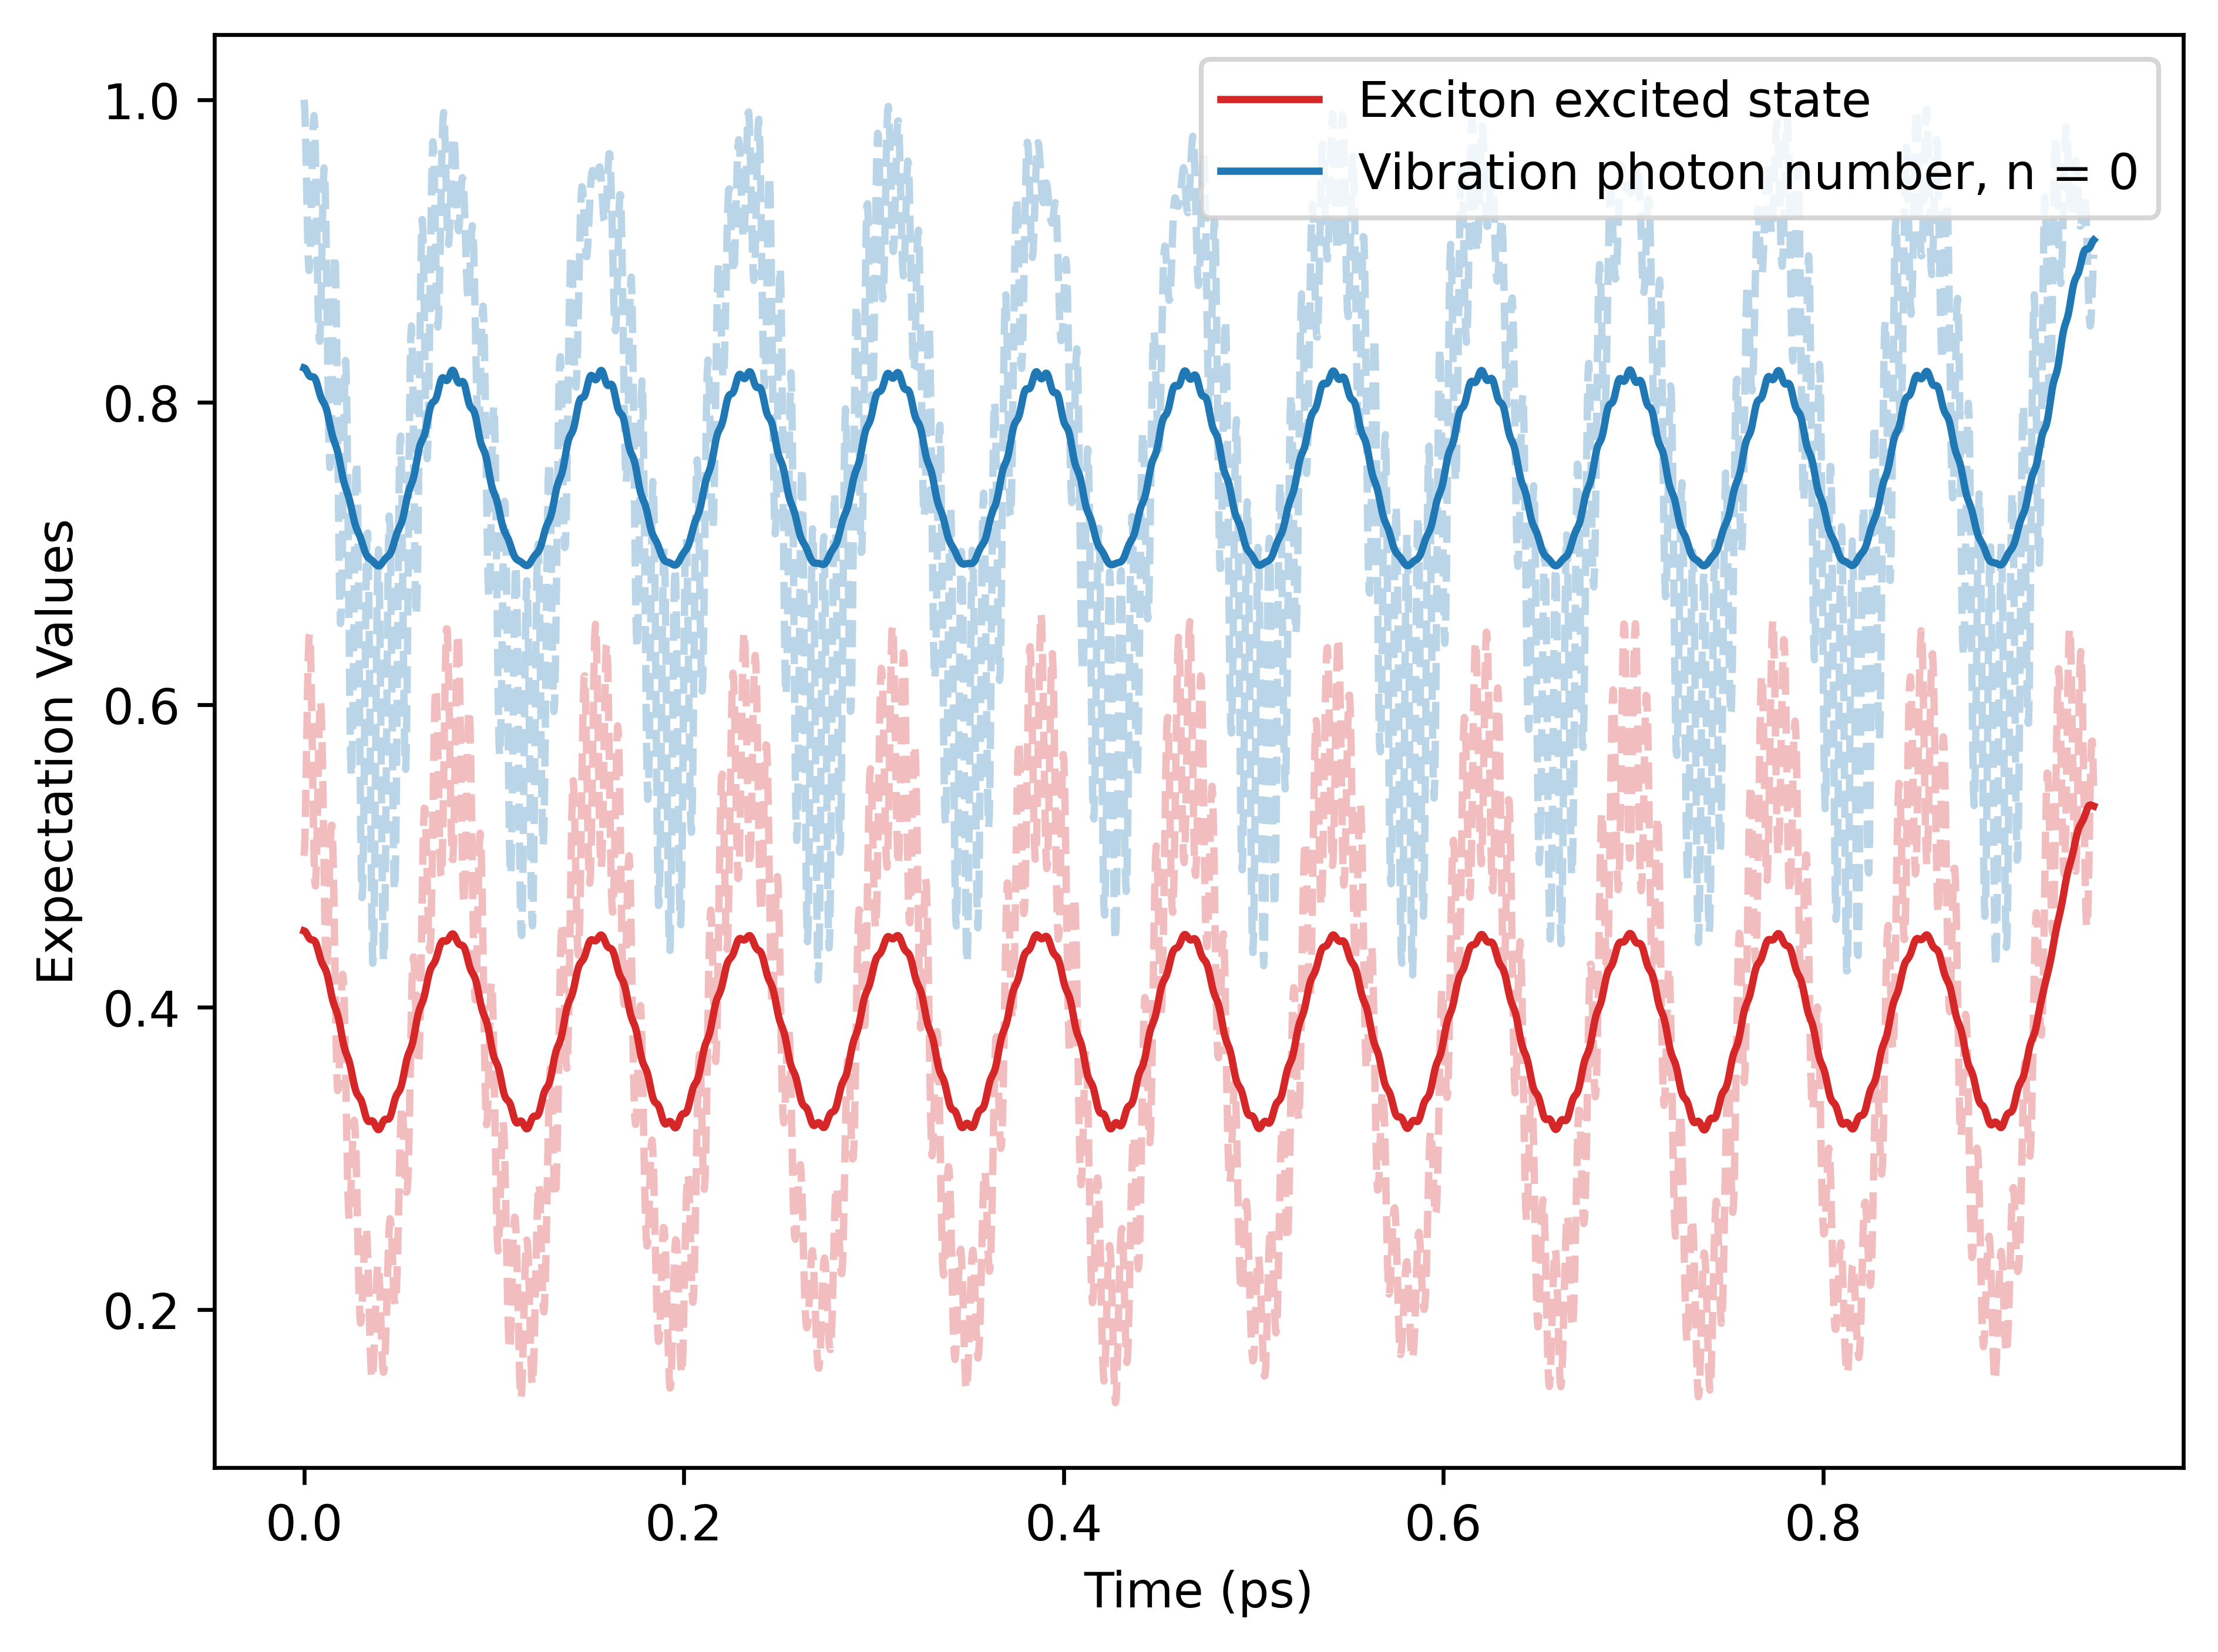
\includegraphics[width=0.49\textwidth]{Research Project/Code/results/ExVib/Closed/Envelope/pops_excited_eg.png}
        \hfill
        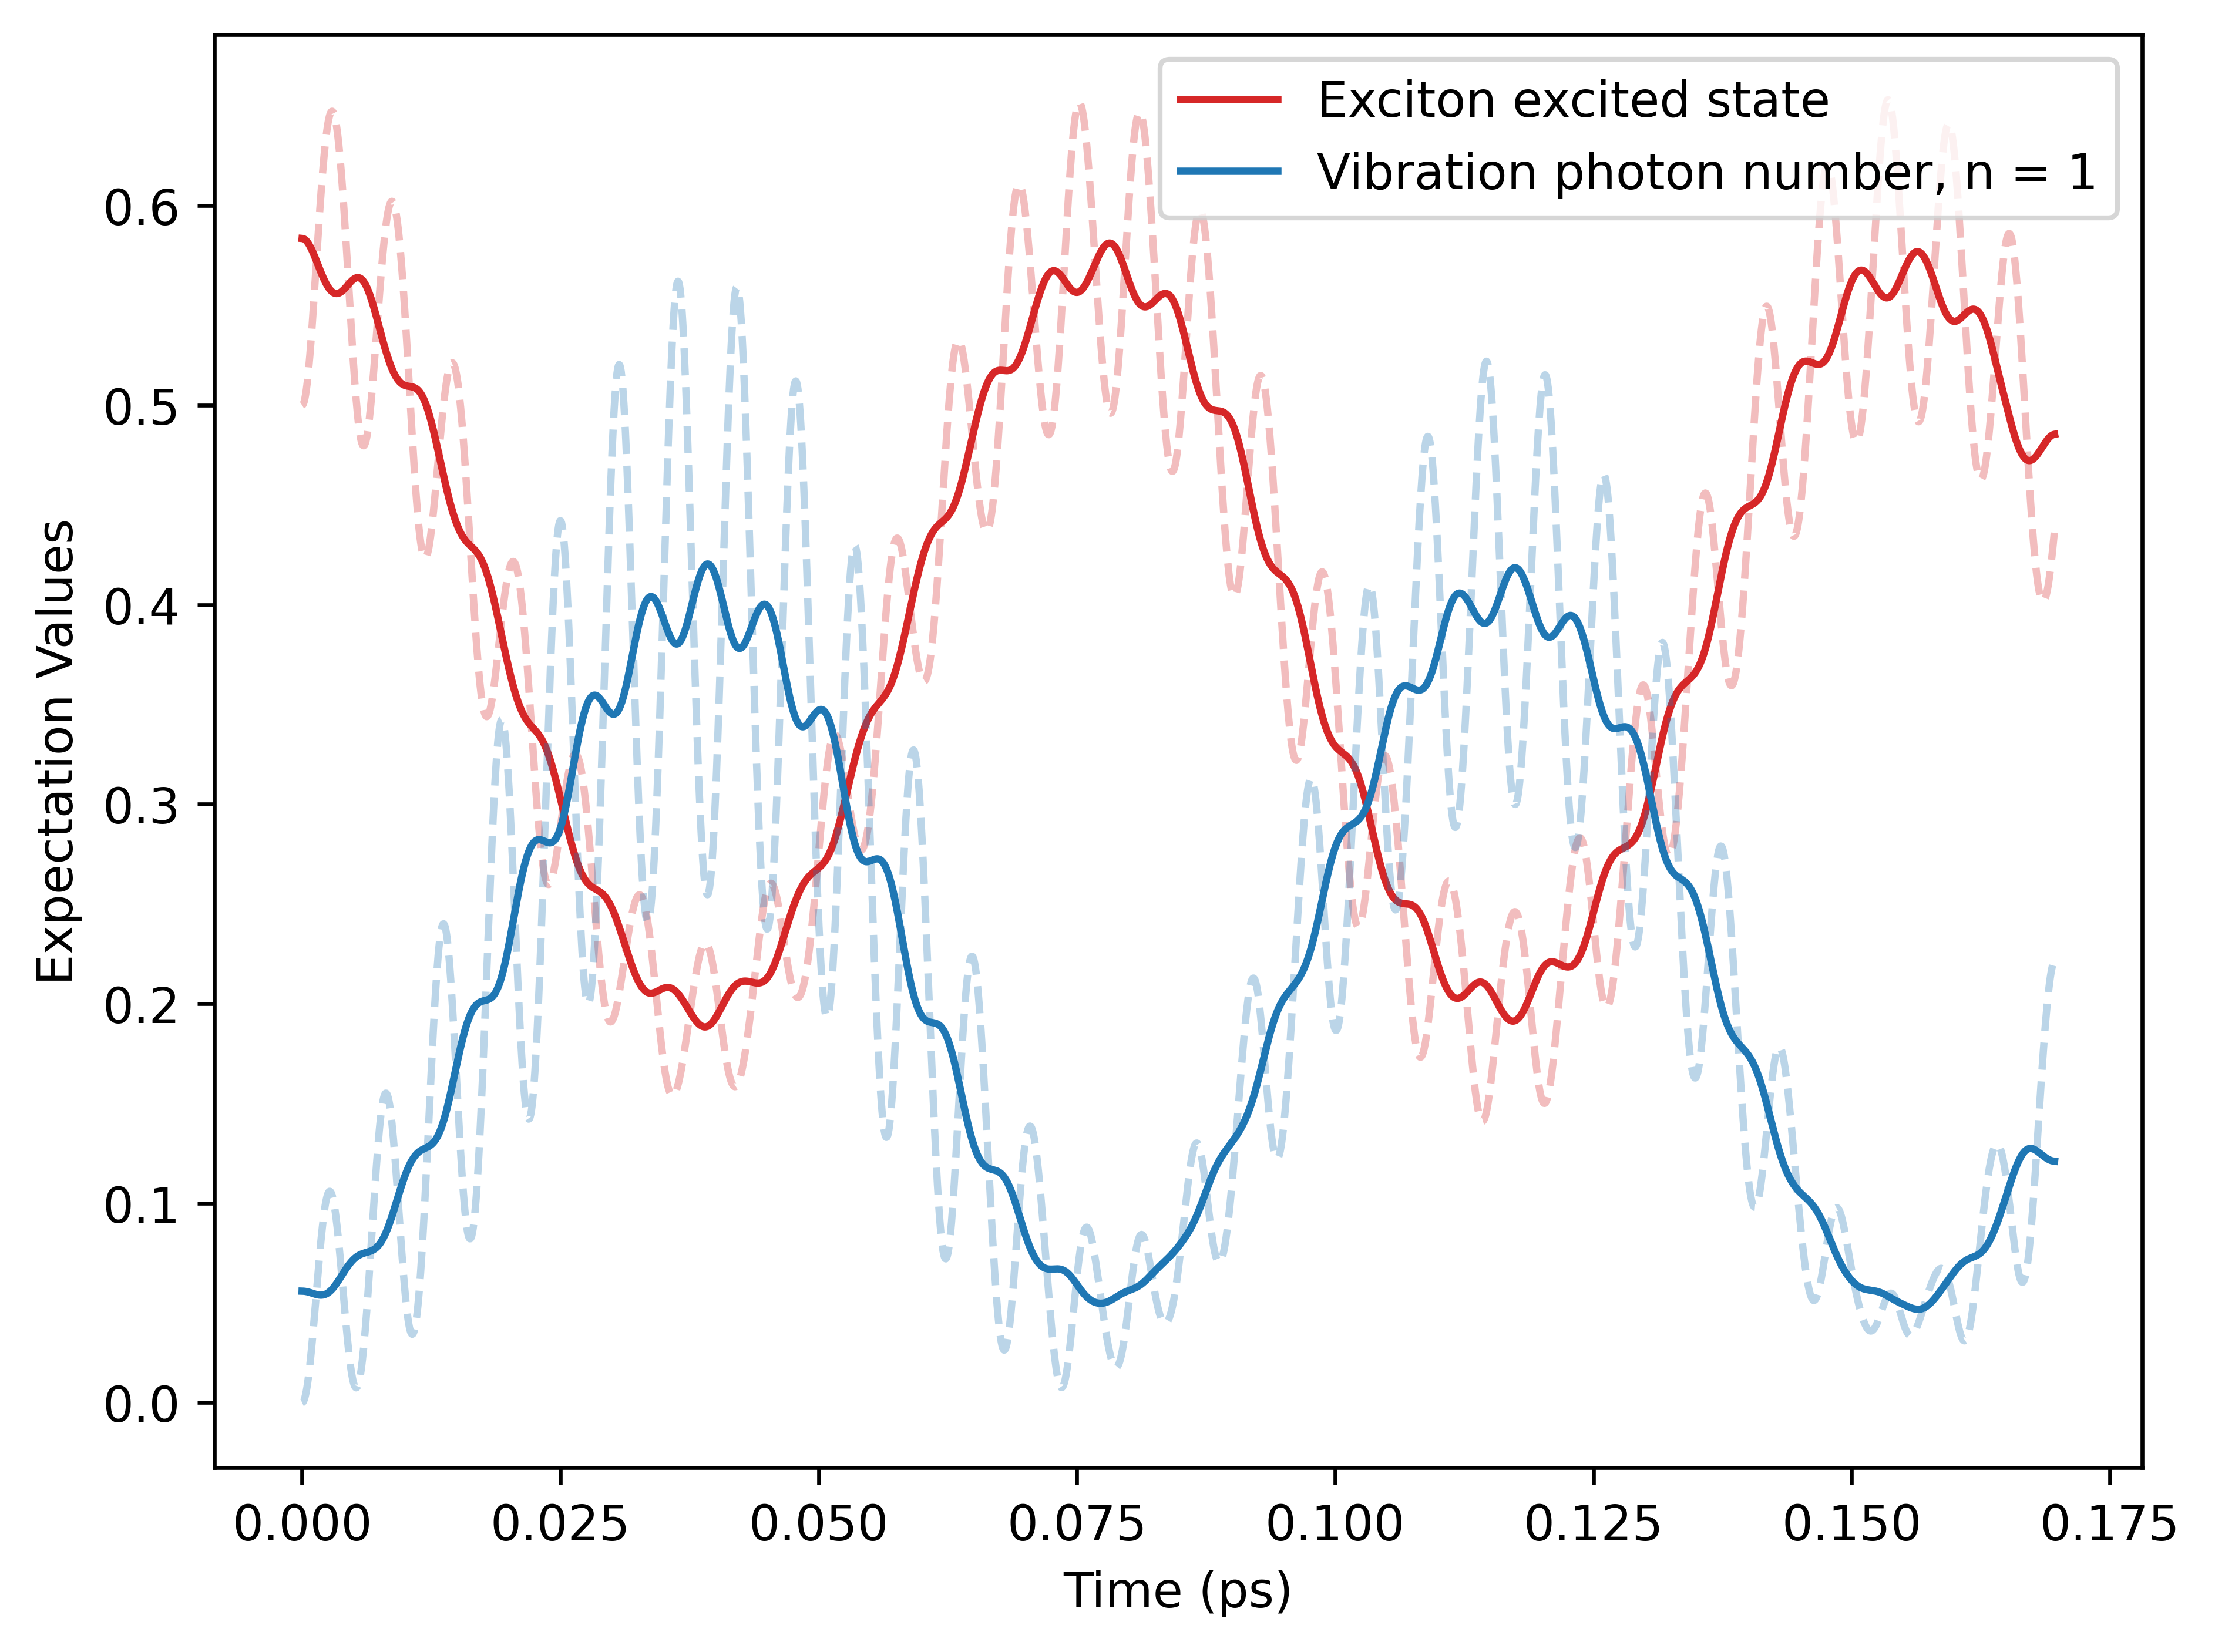
\includegraphics[width=0.49\textwidth]{Research Project/Code/results/ExVib/Closed/Fast/pops_excited_eg.png}
        \caption{}
        \label{fig:EVM_CQS_Pop_eg}
    \end{subfigure}

    \vspace{0.8em}

    % -------- Row (b): Entanglement --------
    \begin{subfigure}{\textwidth}
        \centering
        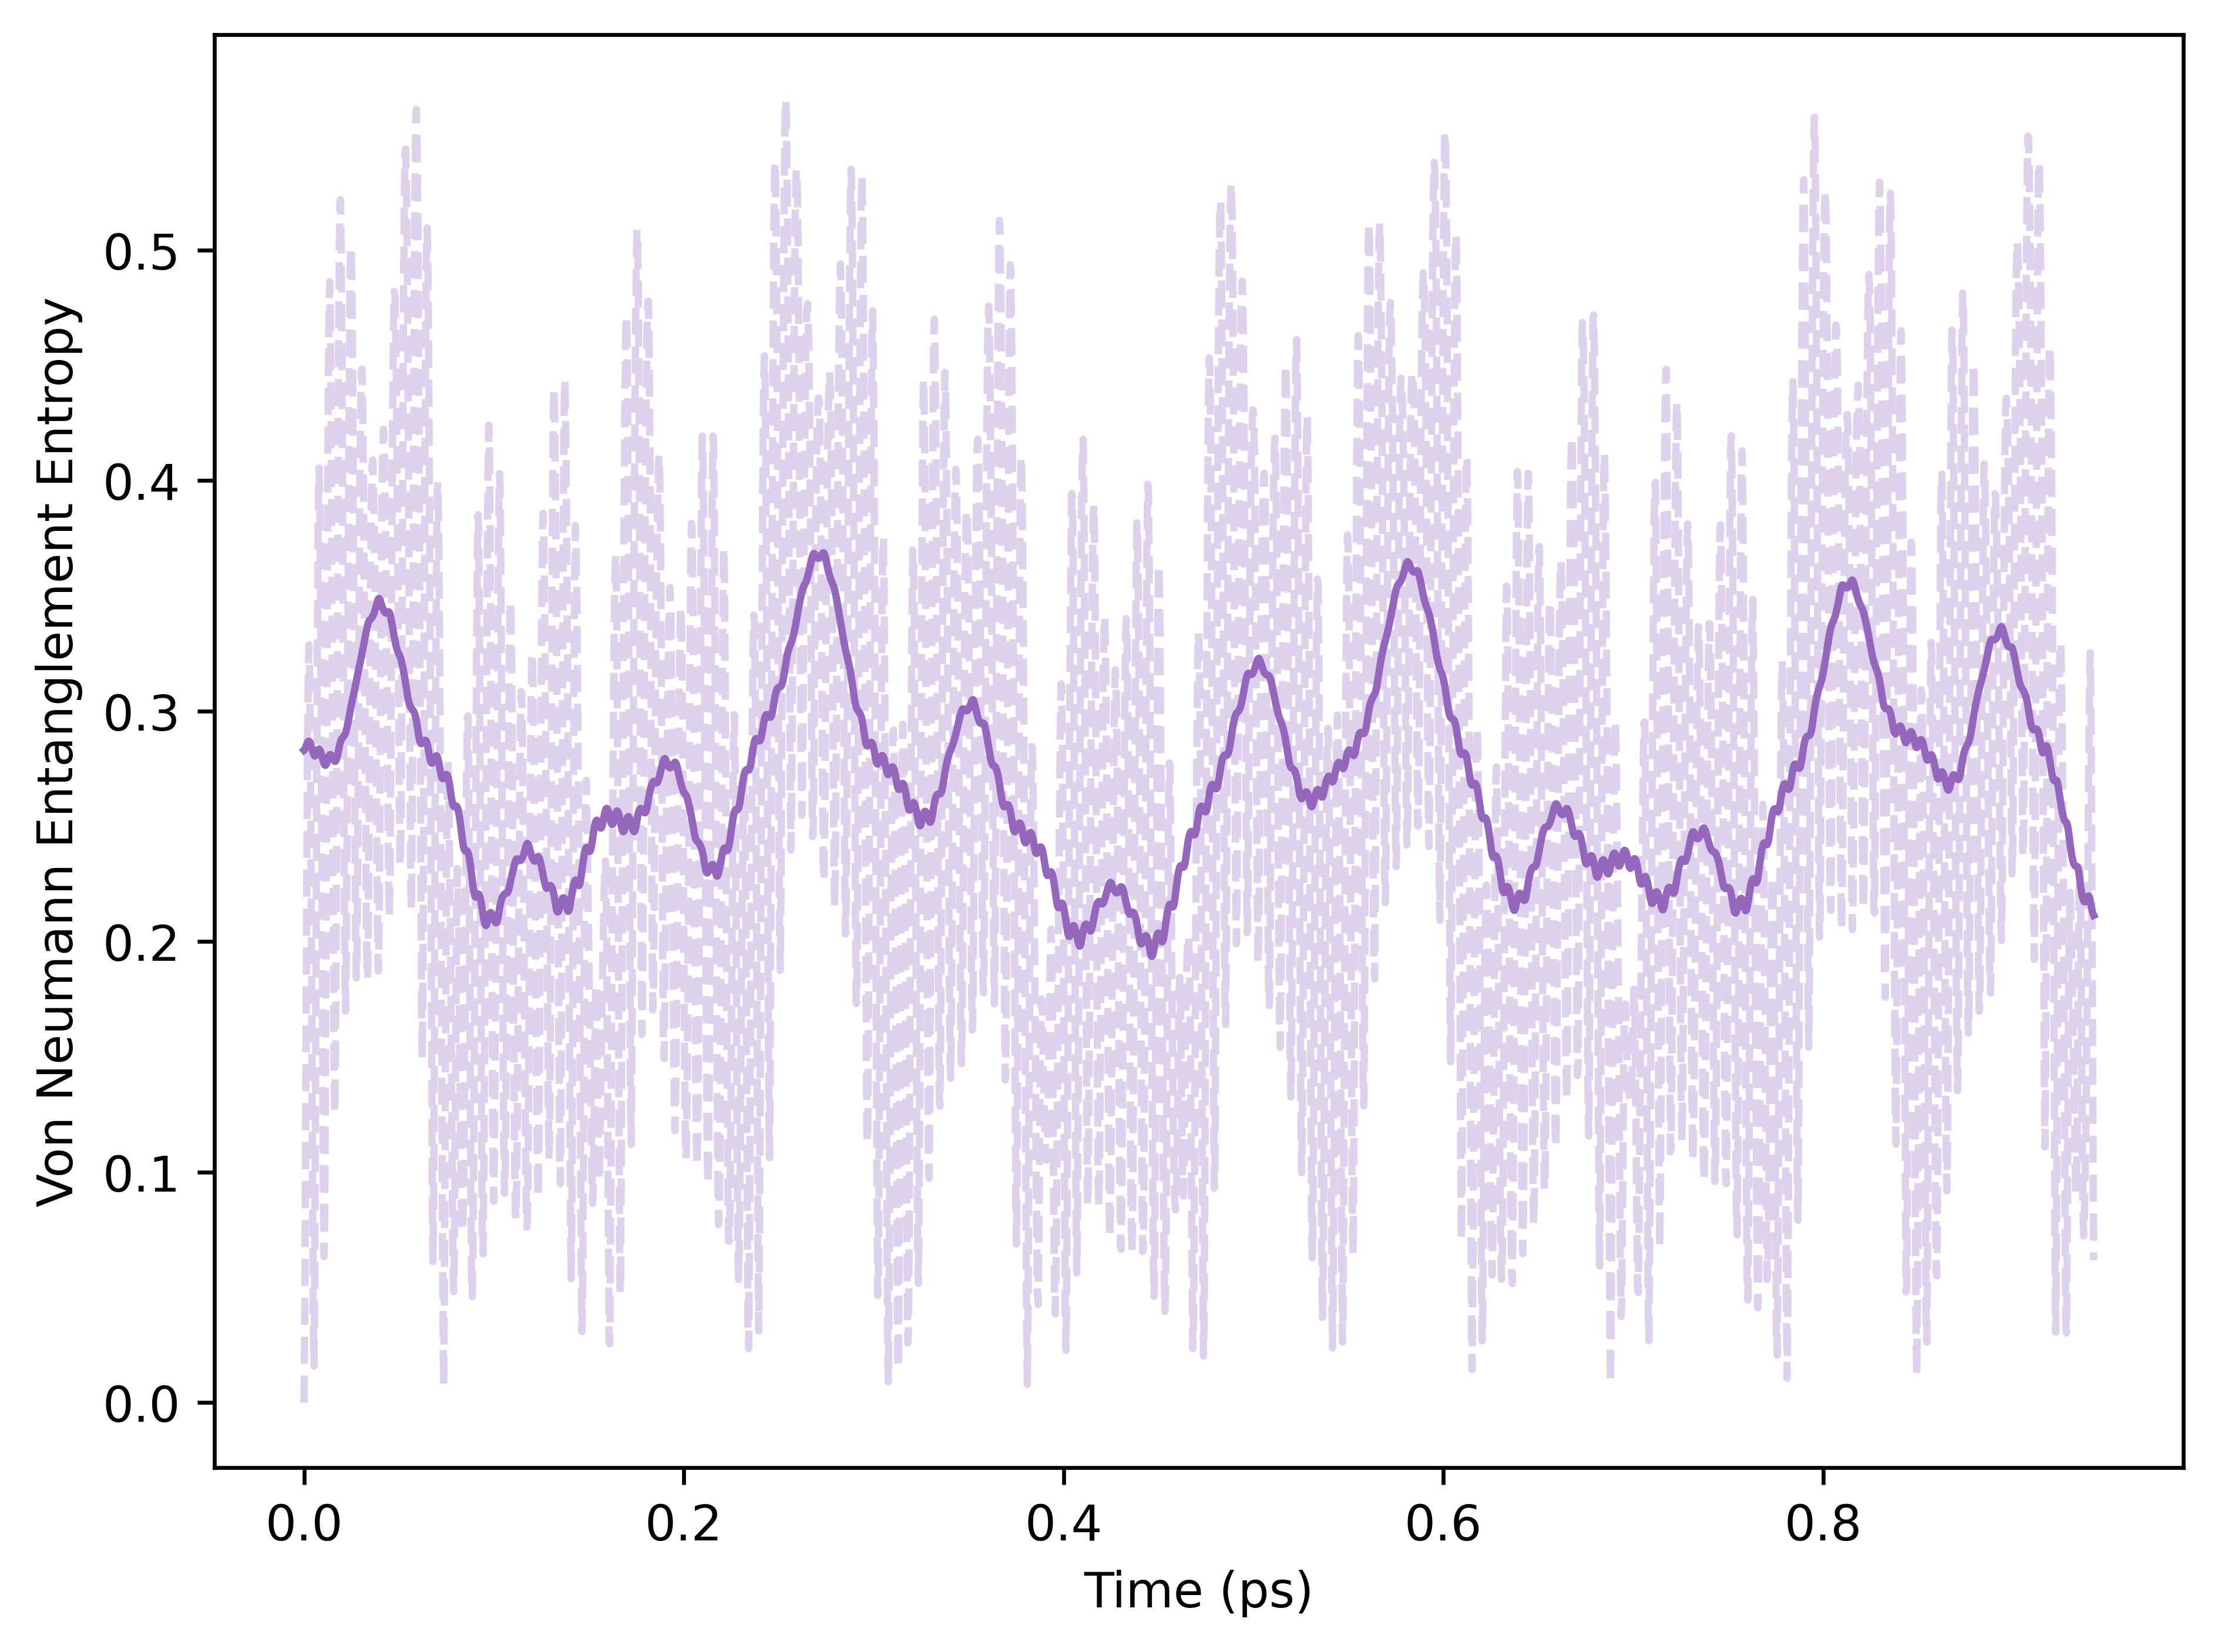
\includegraphics[width=0.49\textwidth]{Research Project/Code/results/ExVib/Closed/Envelope/vne_eg.png}
        \hfill
        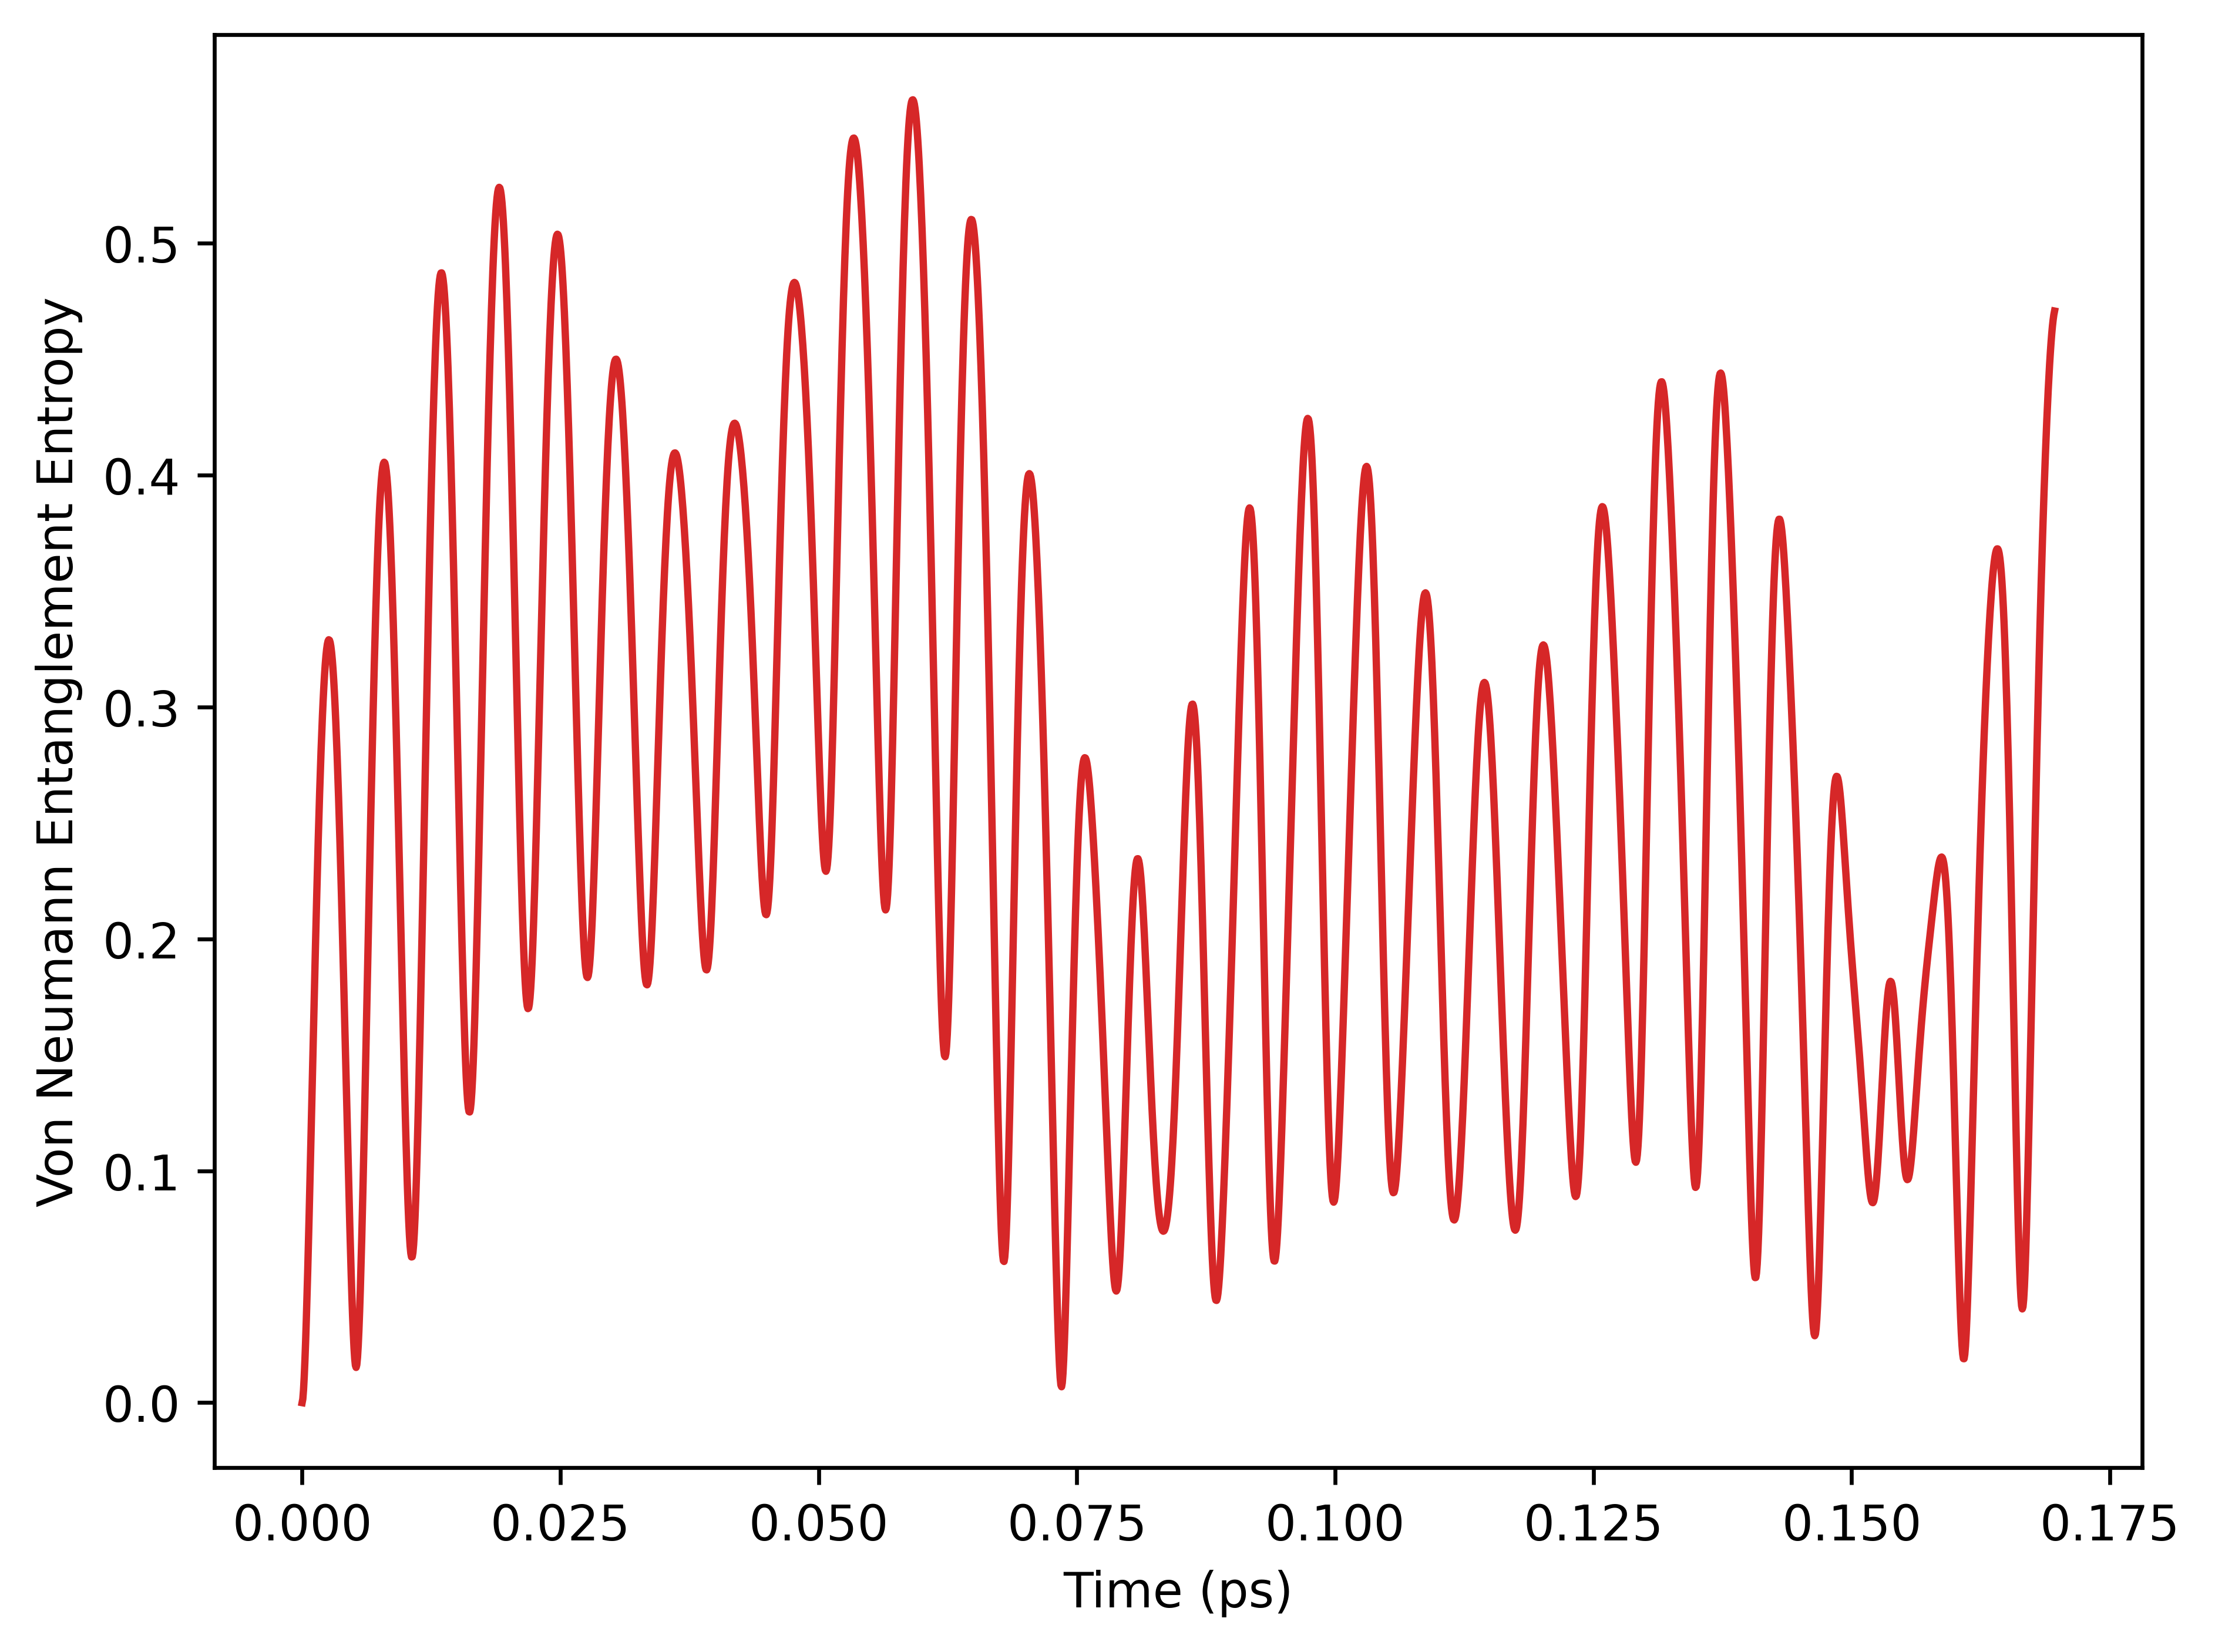
\includegraphics[width=0.49\textwidth]{Research Project/Code/results/ExVib/Closed/Fast/vne_eg.png}
        \caption{}
        \label{fig:EVM_CQS_ent_eg}
    \end{subfigure}

    \vspace{0.8em}

    % -------- Row (c): Coherence --------
    \begin{subfigure}{\textwidth}
        \centering
        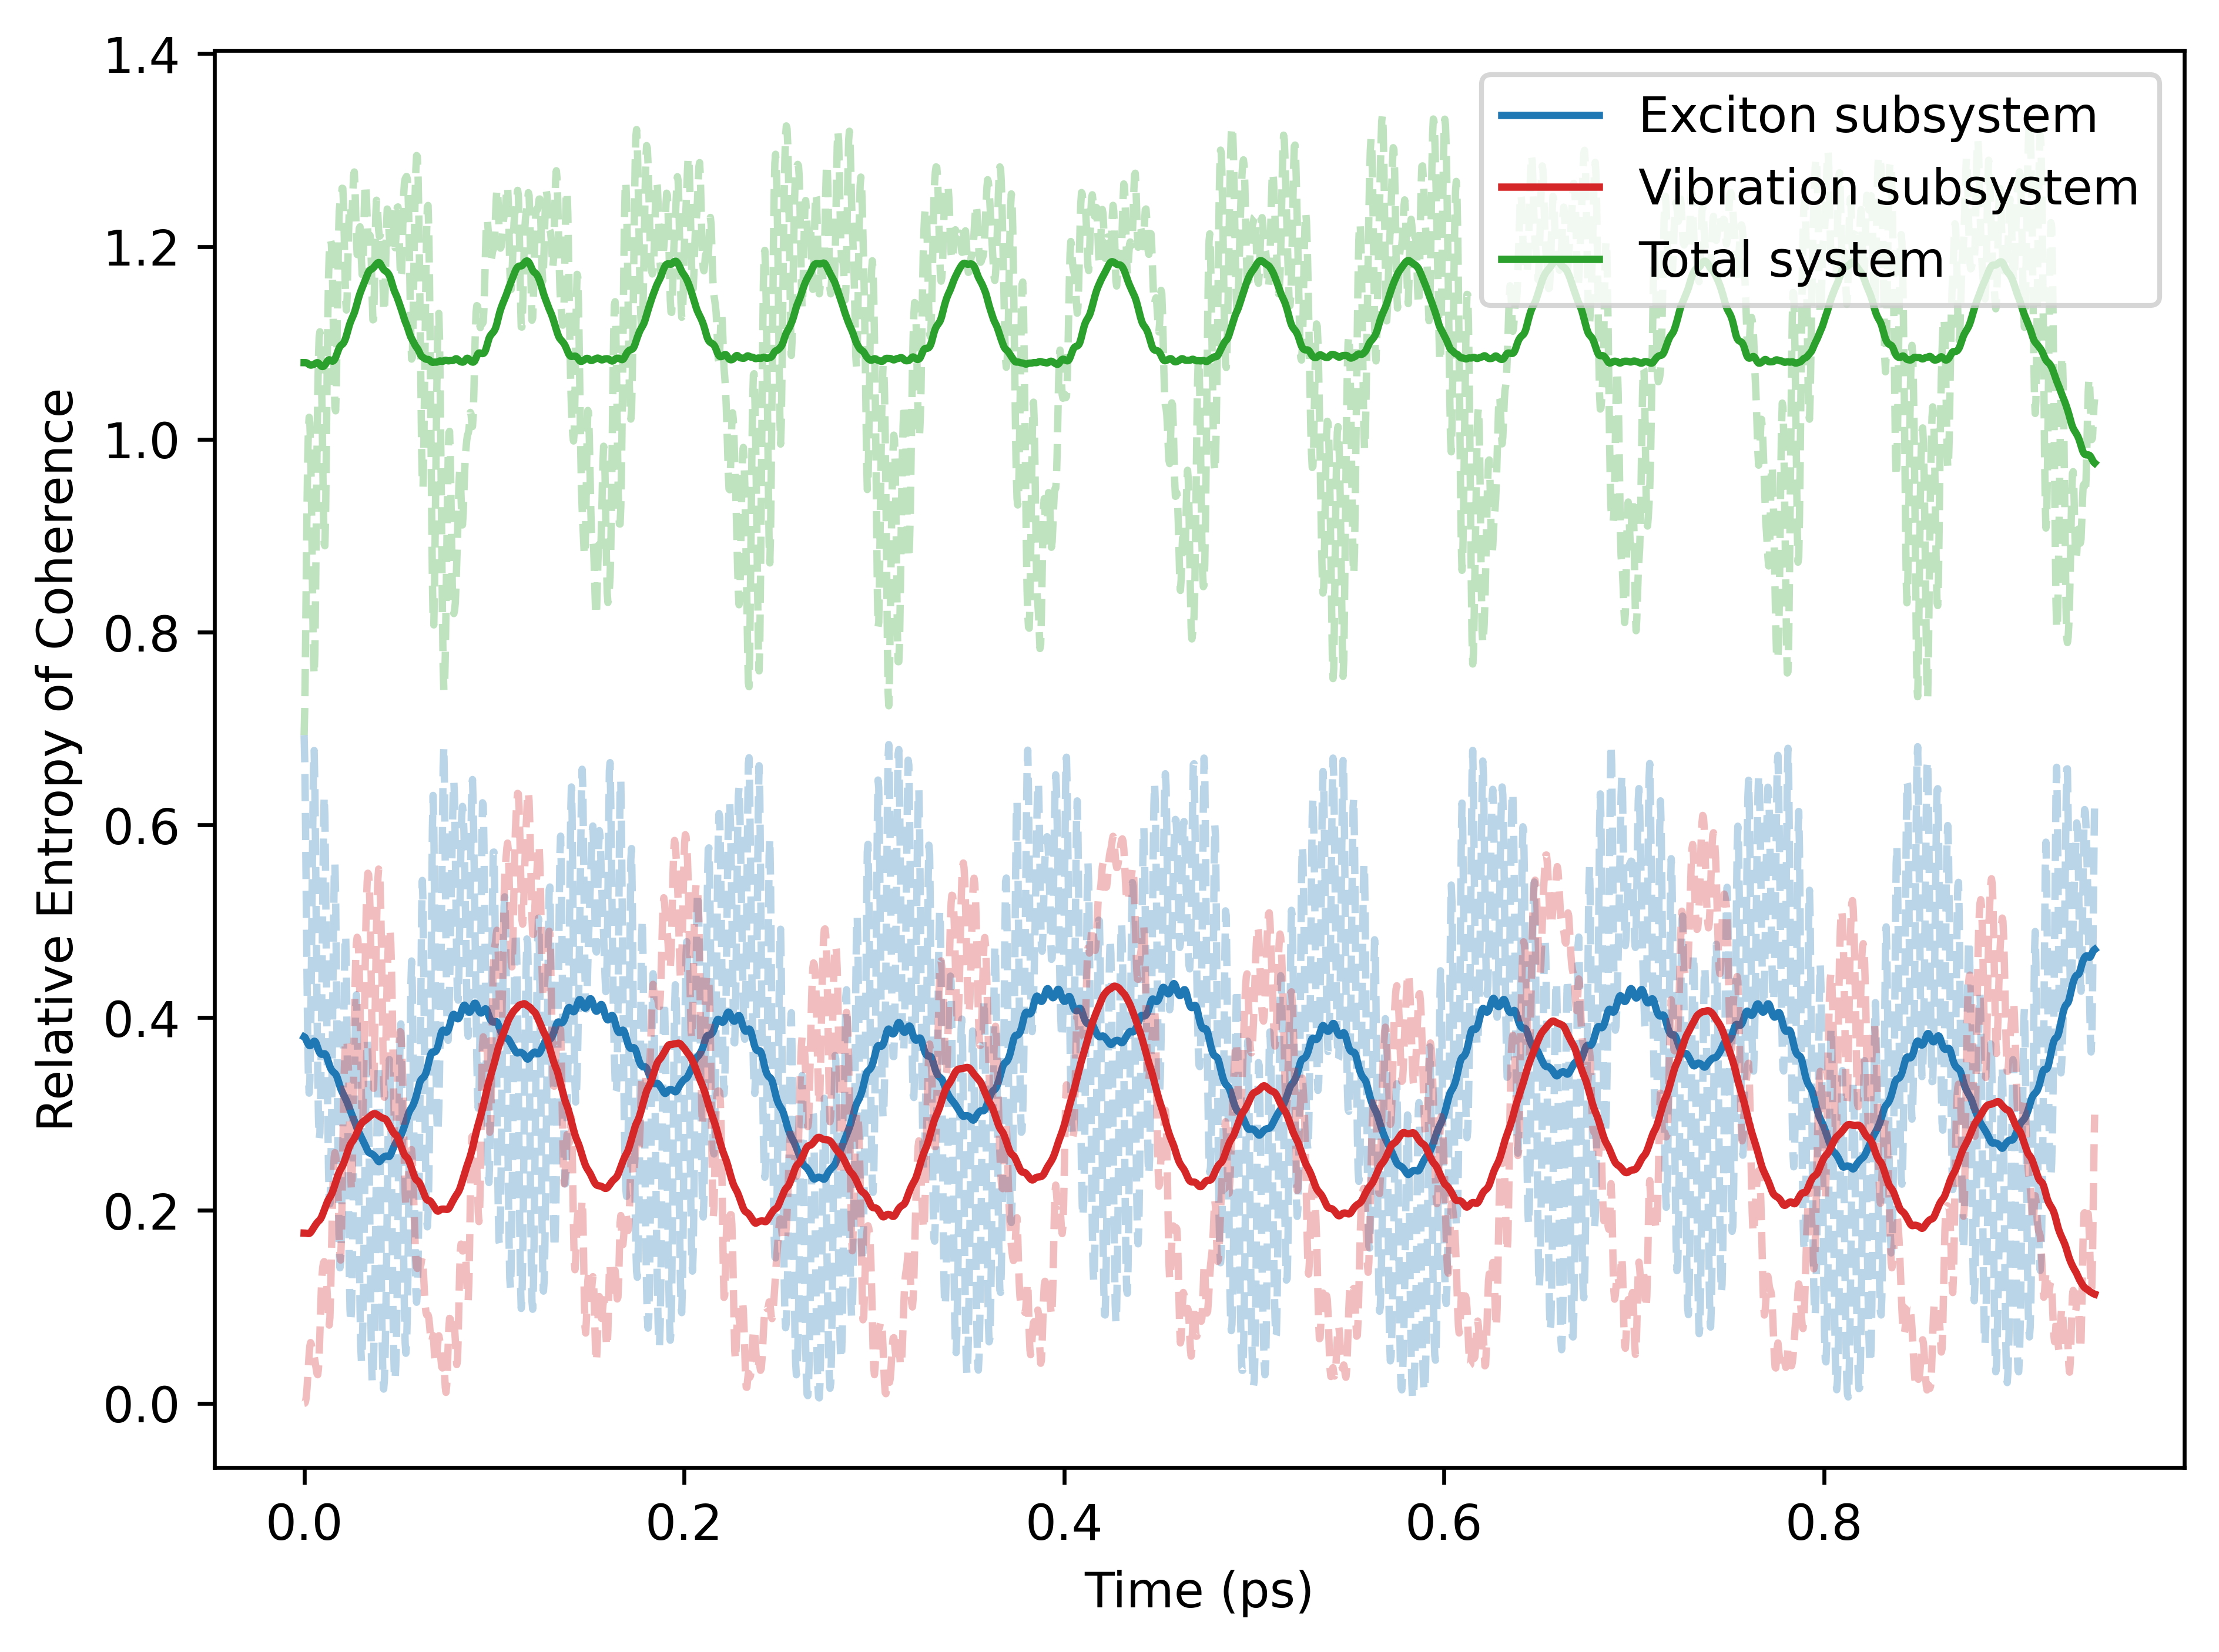
\includegraphics[width=0.49\textwidth]{Research Project/Code/results/ExVib/Closed/Envelope/coh_eg.png}
        \hfill
        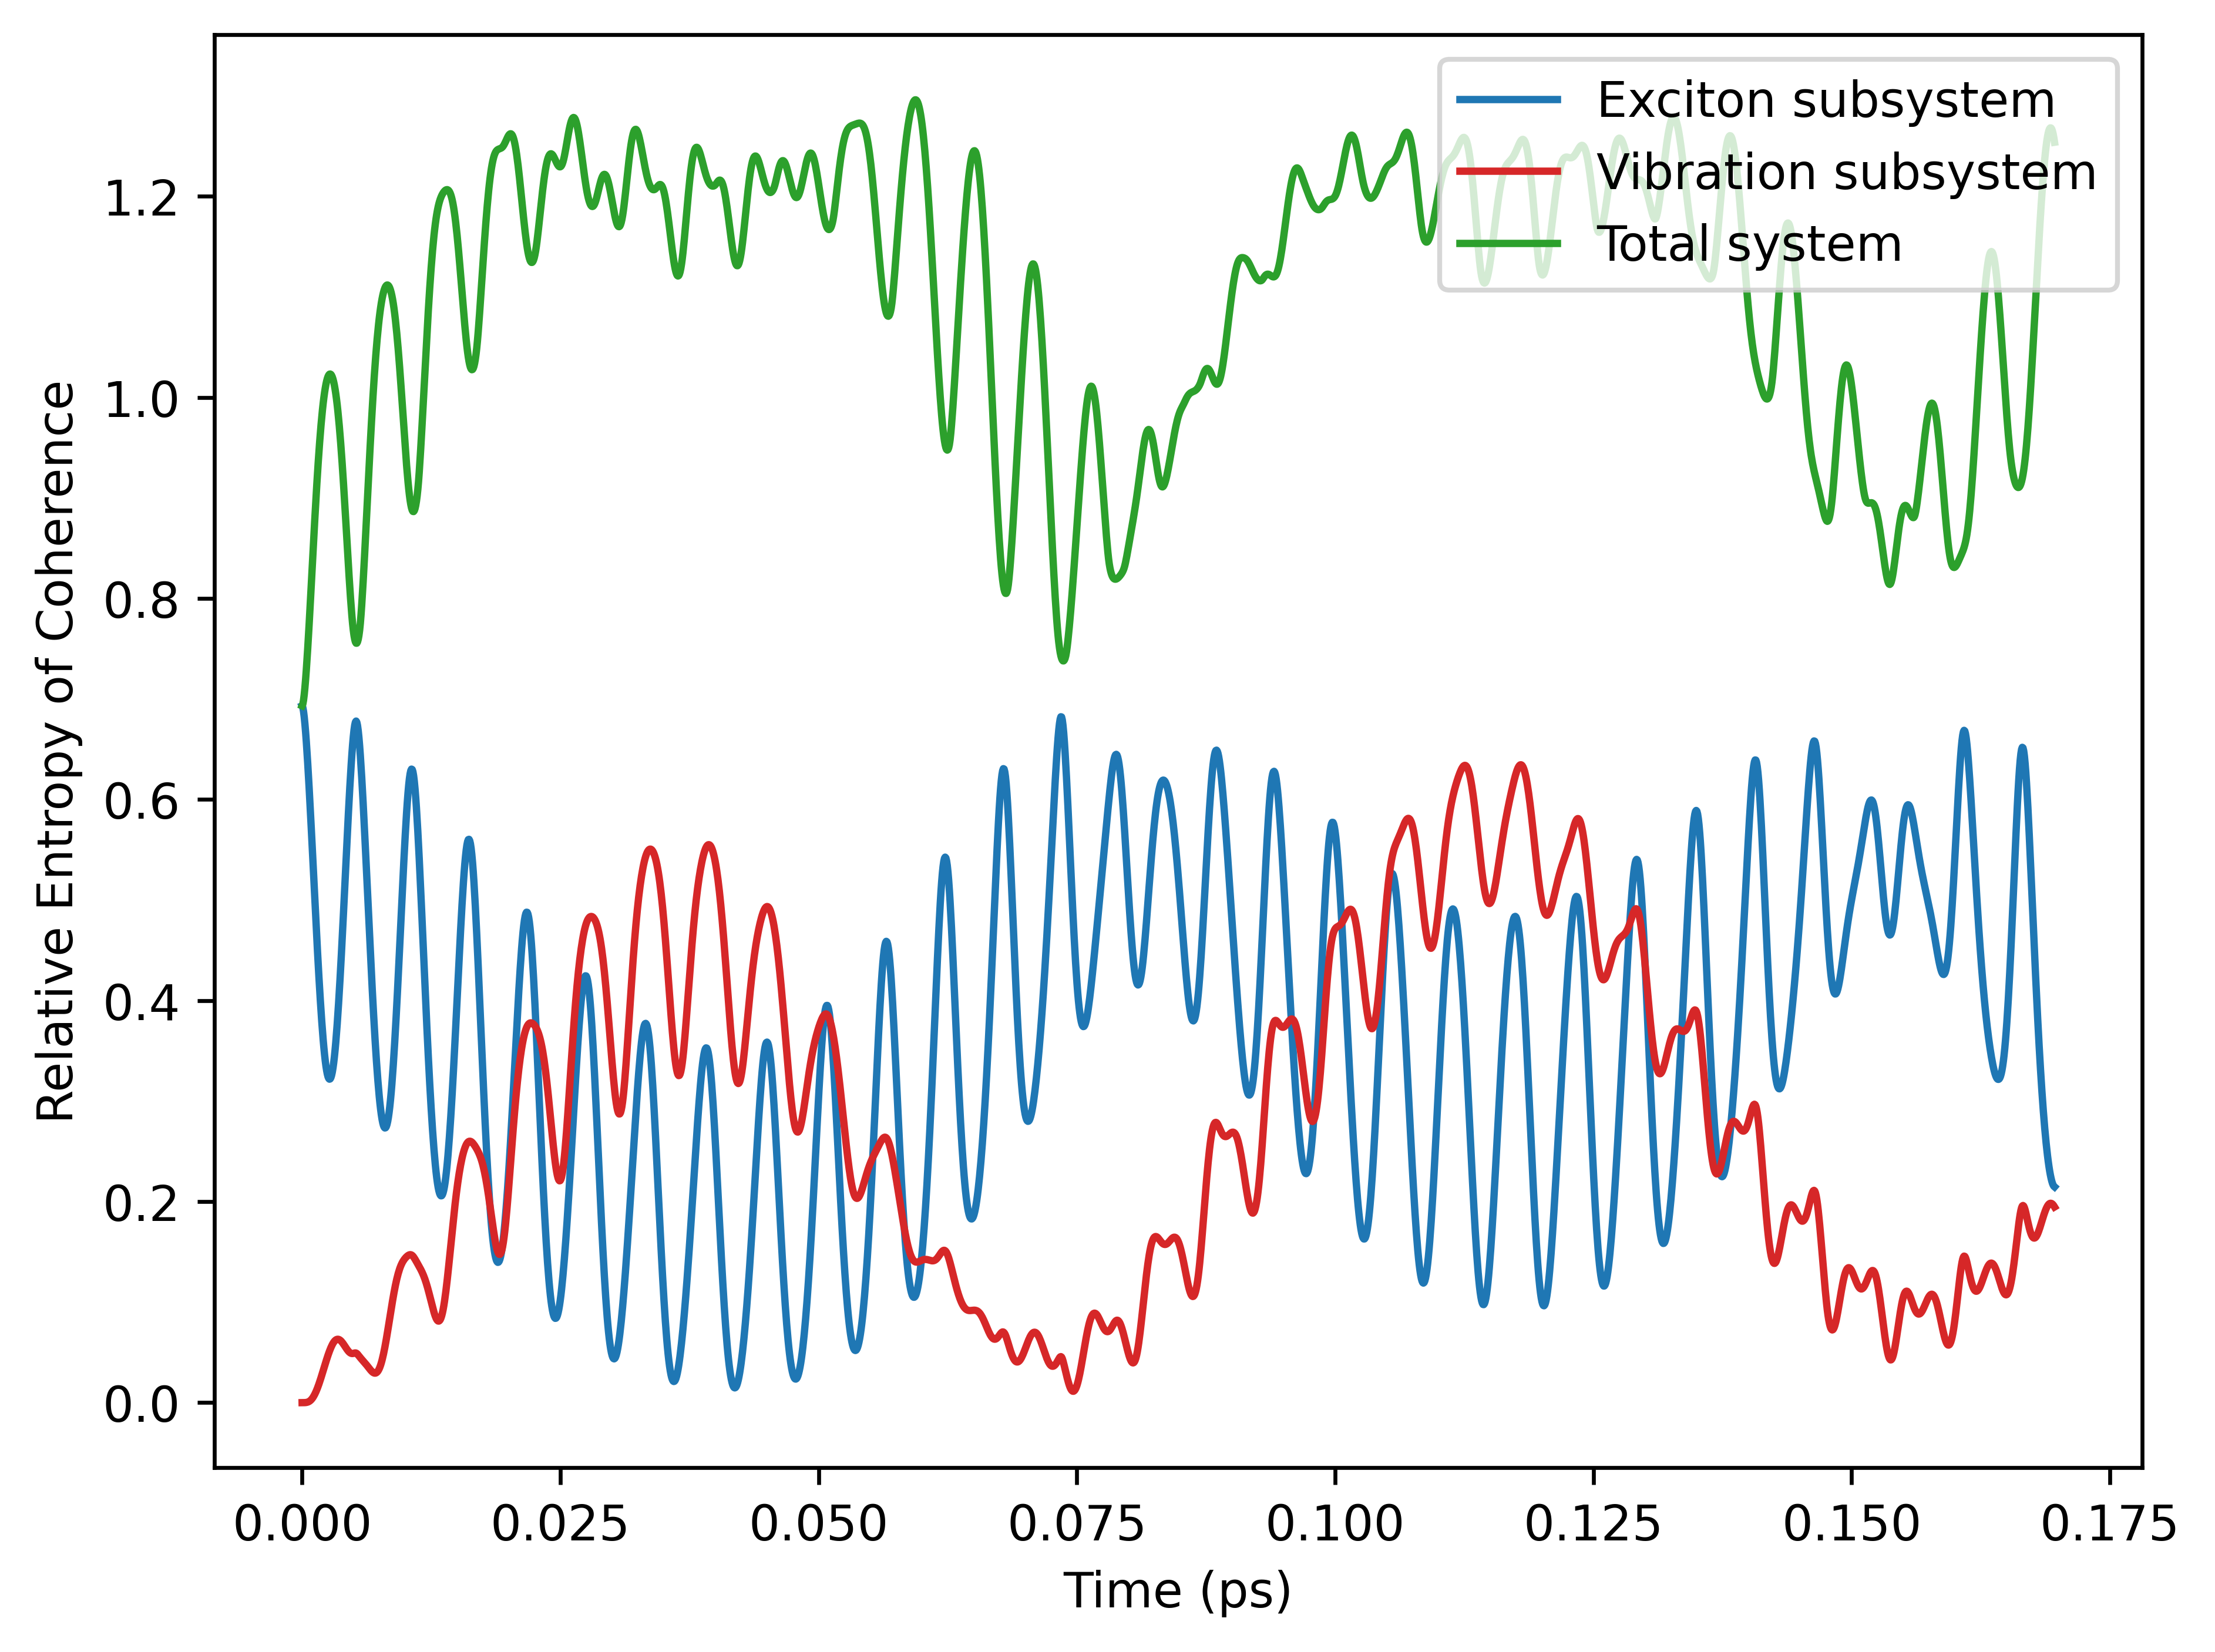
\includegraphics[width=0.49\textwidth]{Research Project/Code/results/ExVib/Closed/Fast/coh_eg.png}
        \caption{}
        \label{fig:EVM_CQS_coh_eg}
    \end{subfigure}

    \caption{Plots of the EVM under closed unitary evolution with an initial state of $|\psi (\text{t=0})\rangle = 1/\sqrt{2}(|1\rangle + |0\rangle)\otimes|n=0\rangle$. The left--hand column of sub--figures is plotted over $\approx$ 1 picosecond to demonstrate envelope and medium frequency oscillations. The right--hand column of sub--figures is plotted over a shorter timescale to demonstrate high frequency oscillations. (a) Populations of the excited exciton state $|1\rangle$ and the vibrational mode, $|n=0\rangle$. (b) Entanglement of the total system, quantified by the von Neumann entropy. (c) Coherence of the two subsystems and total system, quantified by the relative entropy of coherence.} 
    \label{fig:EVM_CQS_eg}
\end{figure}

\noindent its initial $|0\rangle$ subsystem state throughout the evolution, albeit oscillating between superpositions itself and other Fock states. Thus, we note that the joint state $|0,0\rangle$ remains present throughout the entire evolution, analogous to the JCM but arising here for different reasons. \\
\\
When looking at entanglement, however, we notice a significant divergence from our previous case. Figure \ref{fig:EVM_CQS_ent_eg} shows the medium oscillations losing their regular sinusoidal form. This occurs because the initial superposition of exciton states enables both to interact with the vibrational modes from the start. Since the coupling acts with opposite signs on the two exciton states $|1\rangle$ and $|0\rangle$, two entangling processes act simultaneously, giving rise to an irregular oscillatory structure. Moreover, we notice a reduction in the maximum value of entanglement by around 0.1. This can be attributed to the $|0,0\rangle$ state being stationary throughout the evolution (and thus behaving like an unentangled product state), effectively diluting entanglement.\\
\\
We further observe the effects of this stationary state in the coherence of both the subsystems and the total system. Figure \ref{fig:EVM_CQS_coh_eg} shows that coherence for all systems are boosted. While the total coherence reaches a maximum increase around 1.3, both the exciton and vibrational subsystems are doubled at certain points in the evolution. The stationary state adds a constant off--diagonal term to the total system, thus generating a baseline coherence. Furthermore, the exciton subsystem now carries more coherence than the vibrational modes, in contrast to our previous case. The initial state is in a superposition of the two exciton basis states, so the exciton starts with strong off--diagonal terms that remain throughout most of the evolution. The local and global minima of the exciton subsystem coherences are directly associated with the complete transfer of populations to the lower exciton state, and are the only points throughout the evolution where exciton coherence is 0. The vibrational mode, by contrast, must generate coherence through exciton--vibration coupling. Thus, if we start our system in an excitonic superposition, the TLS retains more local coherence than the vibrational mode. On the other hand, if we start in an excitonic eigenstate, the vibrational mode is a better subsystem for carrying coherence. \\
\\
We have completed our analysis of population, entanglement and coherence dynamics under closed evolution, and have observed some key features of the EVM: its three--tier population oscillations, its ability to generate subsystem coherence from classically--behaving initial states such as $|1,0\rangle$, and its potential to boost the exciton subsystem's maximal coherence if we start in an excitonic superposition. We now turn to open system dynamics, where we observe these dynamics again under the effects of decoherence and dissipation.
%%%%%%%%%%%%%%%%%%%%%%%%%%% OQS EVM %%%%%%%%%%%%%%%%%%%%%%%%%%%%%%%%%%
\subsubsection{Open Evolution}

For all open system evolution simulations, we focus on the vibrational mode $|n=1\rangle$, contrary to our closed evolution simulations, to provide a clearer visualisation of the effects of decoherence and dissipation. As before, all datasets are smoothed to aid visualisation, and each result is presented on both long and short timescales to highlight the fine--grain dynamics of the EVM.

\subsubsubsection{Case I: Excited State Initial Condition}

We begin with analysis of the population, entanglement and coherence dynamics for the initial condition in equation \ref{eqn:init_EVM_e0}.\\
\\
The population dynamics in Figure \ref{fig:EVM_OQS_Pop_e0} exhibit the expected hierarchy of oscillations across all three dissipative processes. When only the spontaneous atomic emission channel is open (Figure \ref{fig:EVM_OQS_Pop_spont_e0}), the exciton subsystem decays from $|1\rangle$ to $|0\rangle$ a faster rate than the vibrational mode $|n=1\rangle$. Conversely, when the thermal dissipation channel is open in isolation (Figure \ref{fig:EVM_OQS_Pop_therm_e0}), the vibration subsystem decays much faster than the exciton excited state. This contrast indicates that the subsystem's interaction is less pronounced than in the JCM, whose subsystems decay at comparable rates. The distinction can be explained by the interaction Hamiltonian of the EVM: $\hat{\sigma}_z$ is coupled to $\hat{b}_{\scriptscriptstyle \text{rd}}^\dagger + \hat{b}_{\scriptscriptstyle \text{rd}}$. The $\hat{\sigma}_z$ term primarily introduces phase shifts to the exciton subsystem, and does not induce population transfer. If the interaction instead involved $\hat{\sigma}_x$, we would observe
%%%%%%%%%%%% POPS %%%%%%%%%%%
\begin{figure}[H]
    \centering

    % -------- Row (a): Spontaneous emission --------
    \begin{subfigure}{\textwidth}
        \centering
        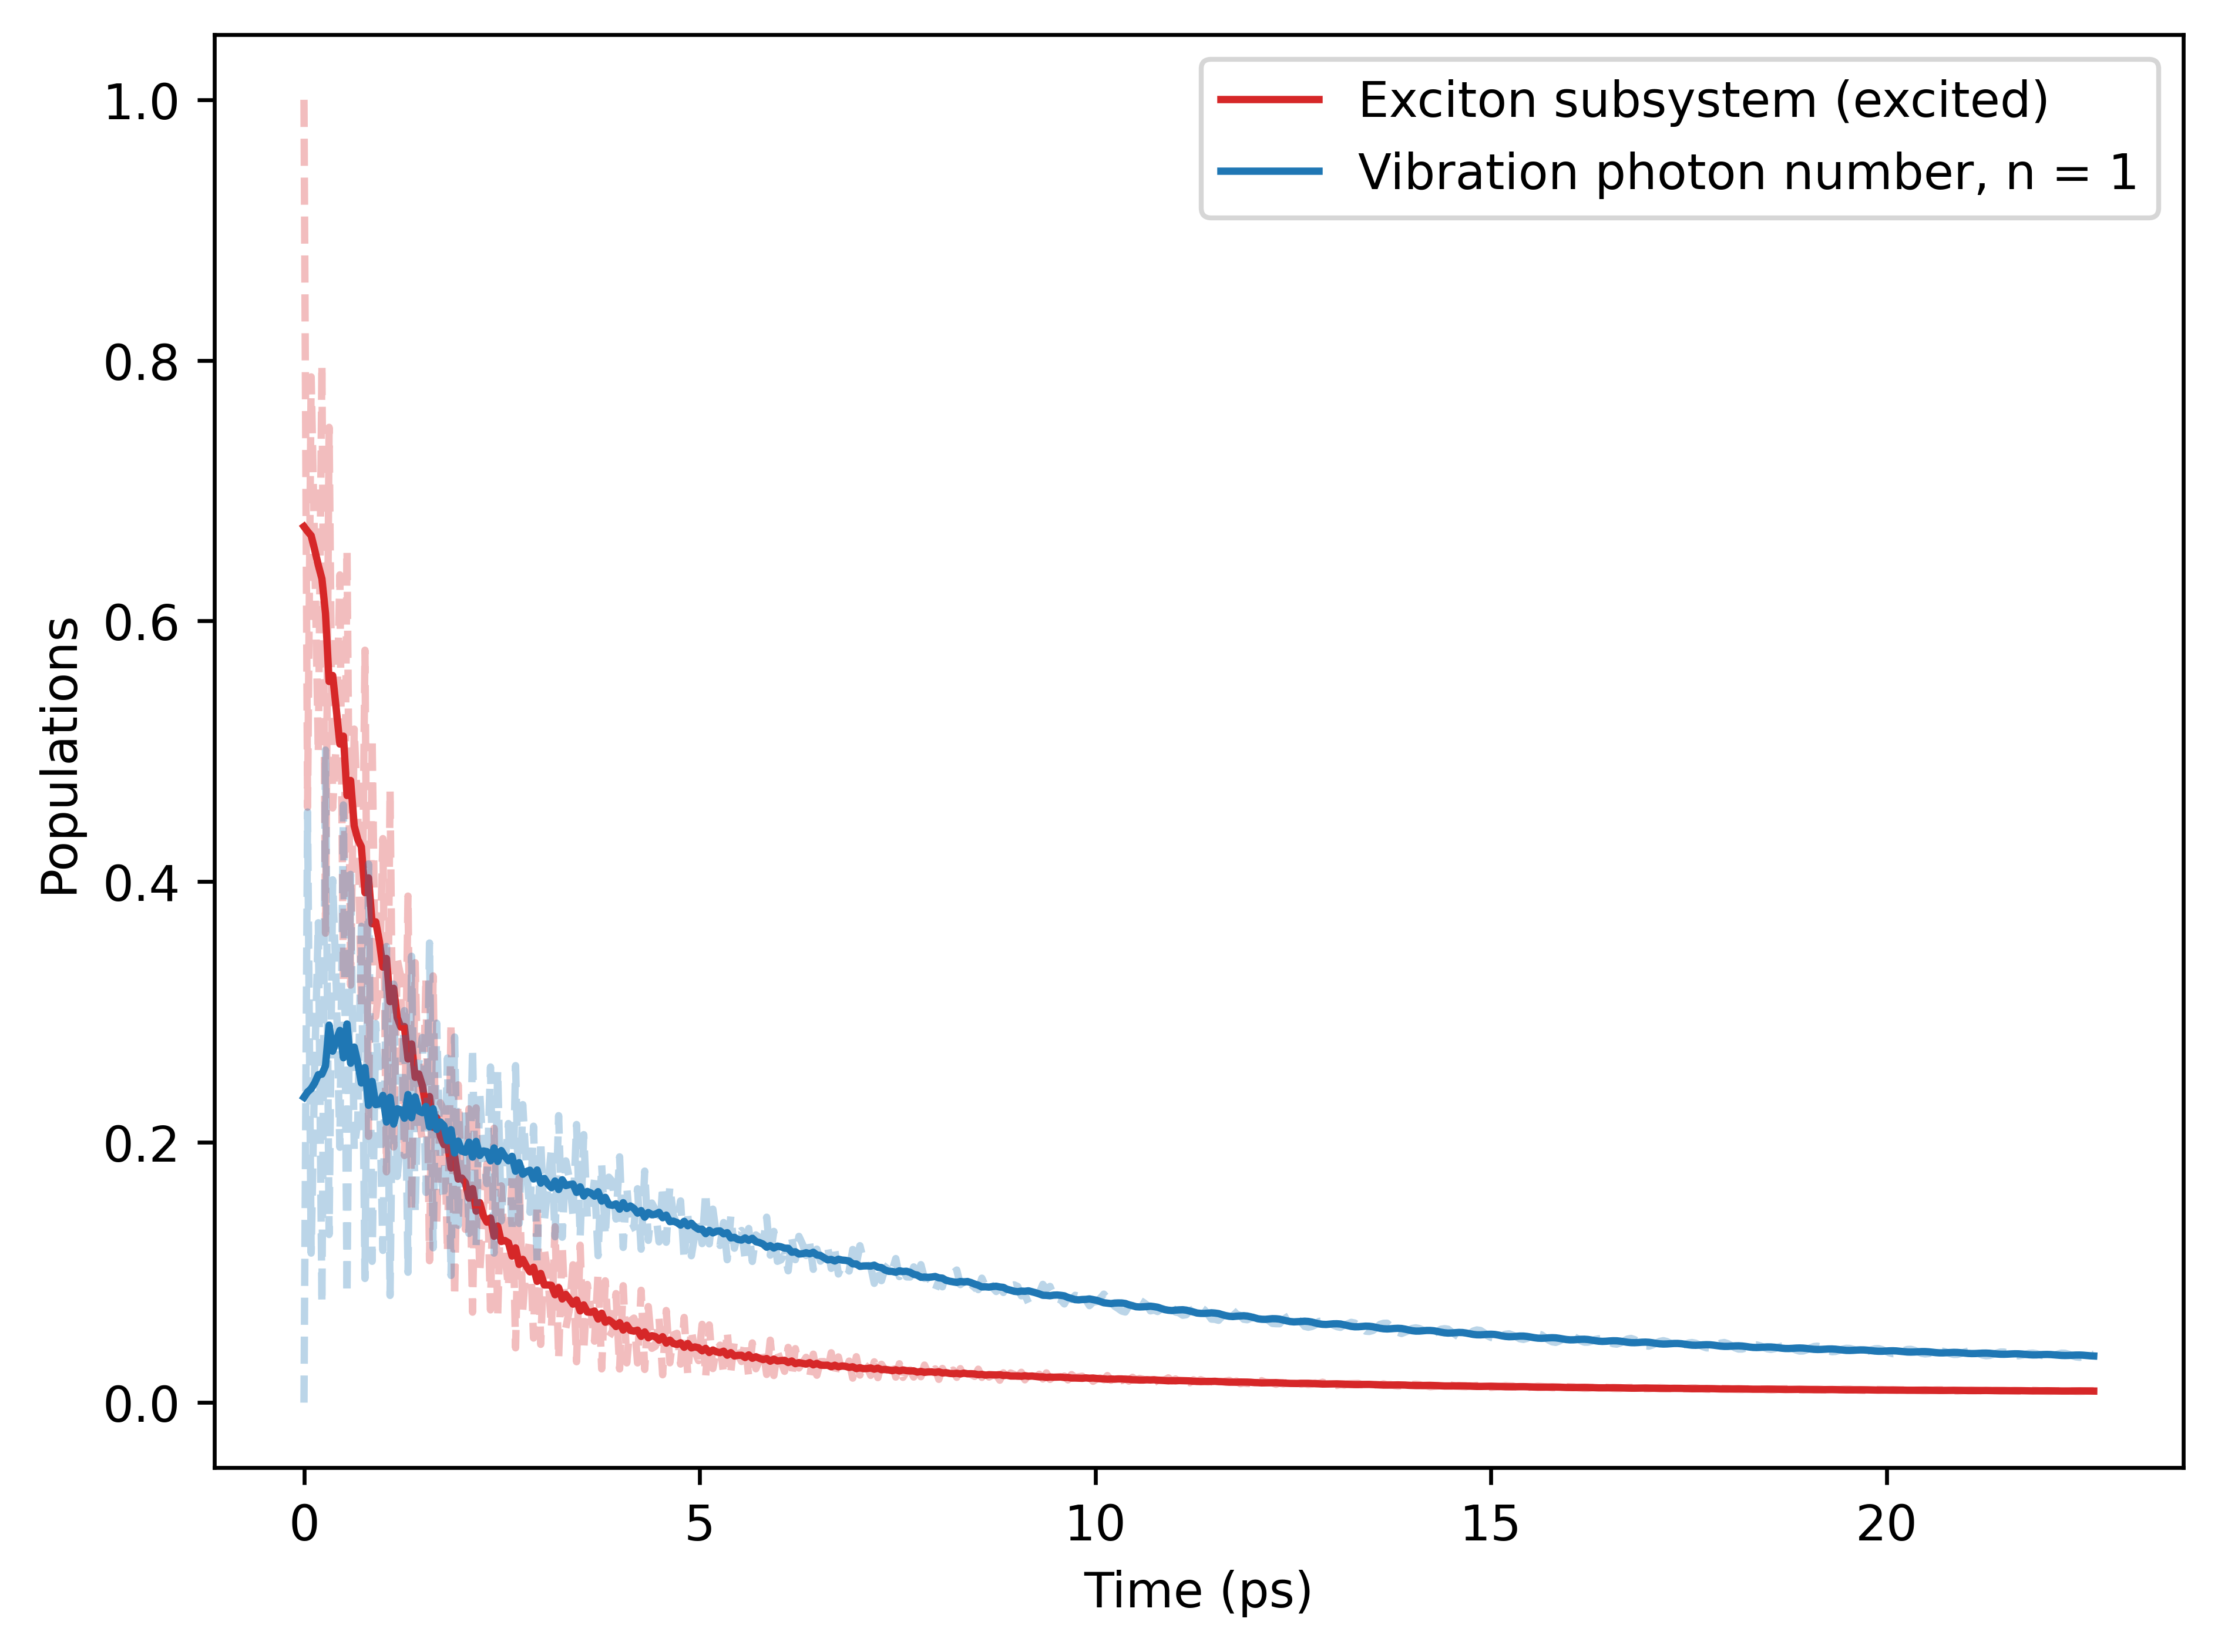
\includegraphics[width=0.49\textwidth]{Research Project/Code/results/ExVib/Open/Population/Envelope/pops_ex_spont_e0.png}
        \hfill
        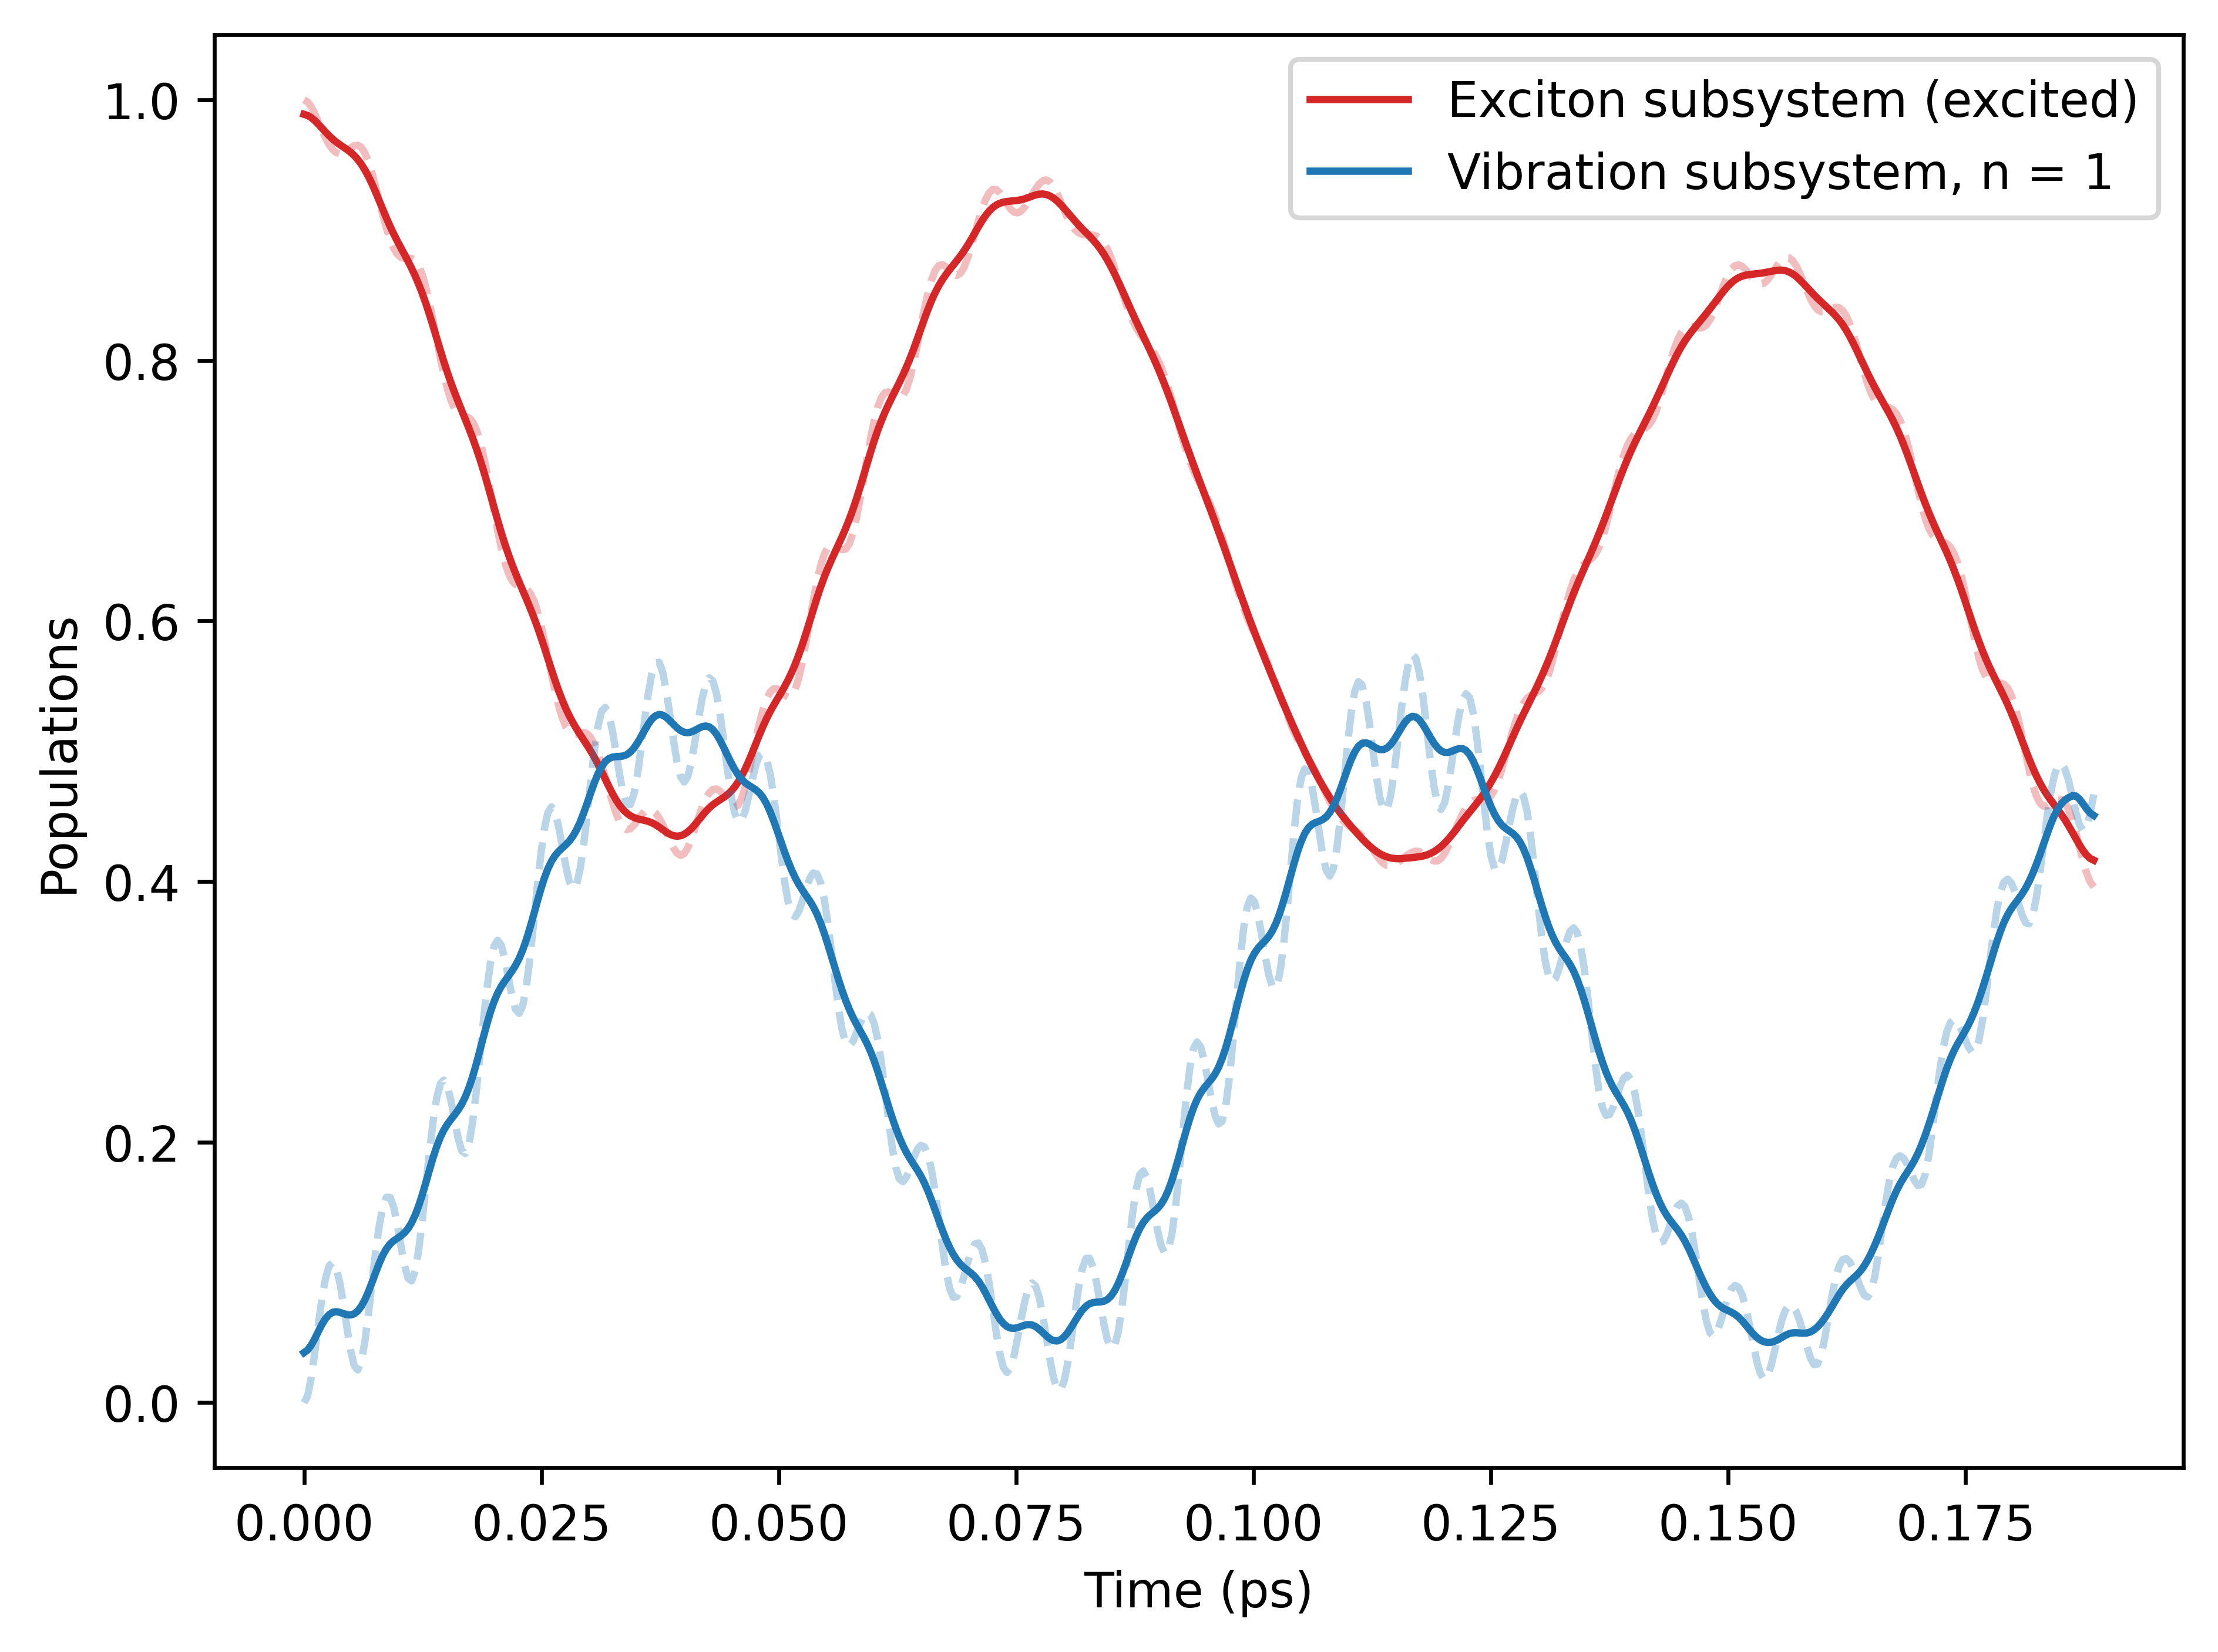
\includegraphics[width=0.49\textwidth]{Research Project/Code/results/ExVib/Open/Population/Fast/pops_ex_spont_e0.png}
        \caption{}
        \label{fig:EVM_OQS_Pop_spont_e0}
    \end{subfigure}

    \vspace{0.8em}

    % -------- Row (b): Thermal dissipation --------
    \begin{subfigure}{\textwidth}
        \centering
        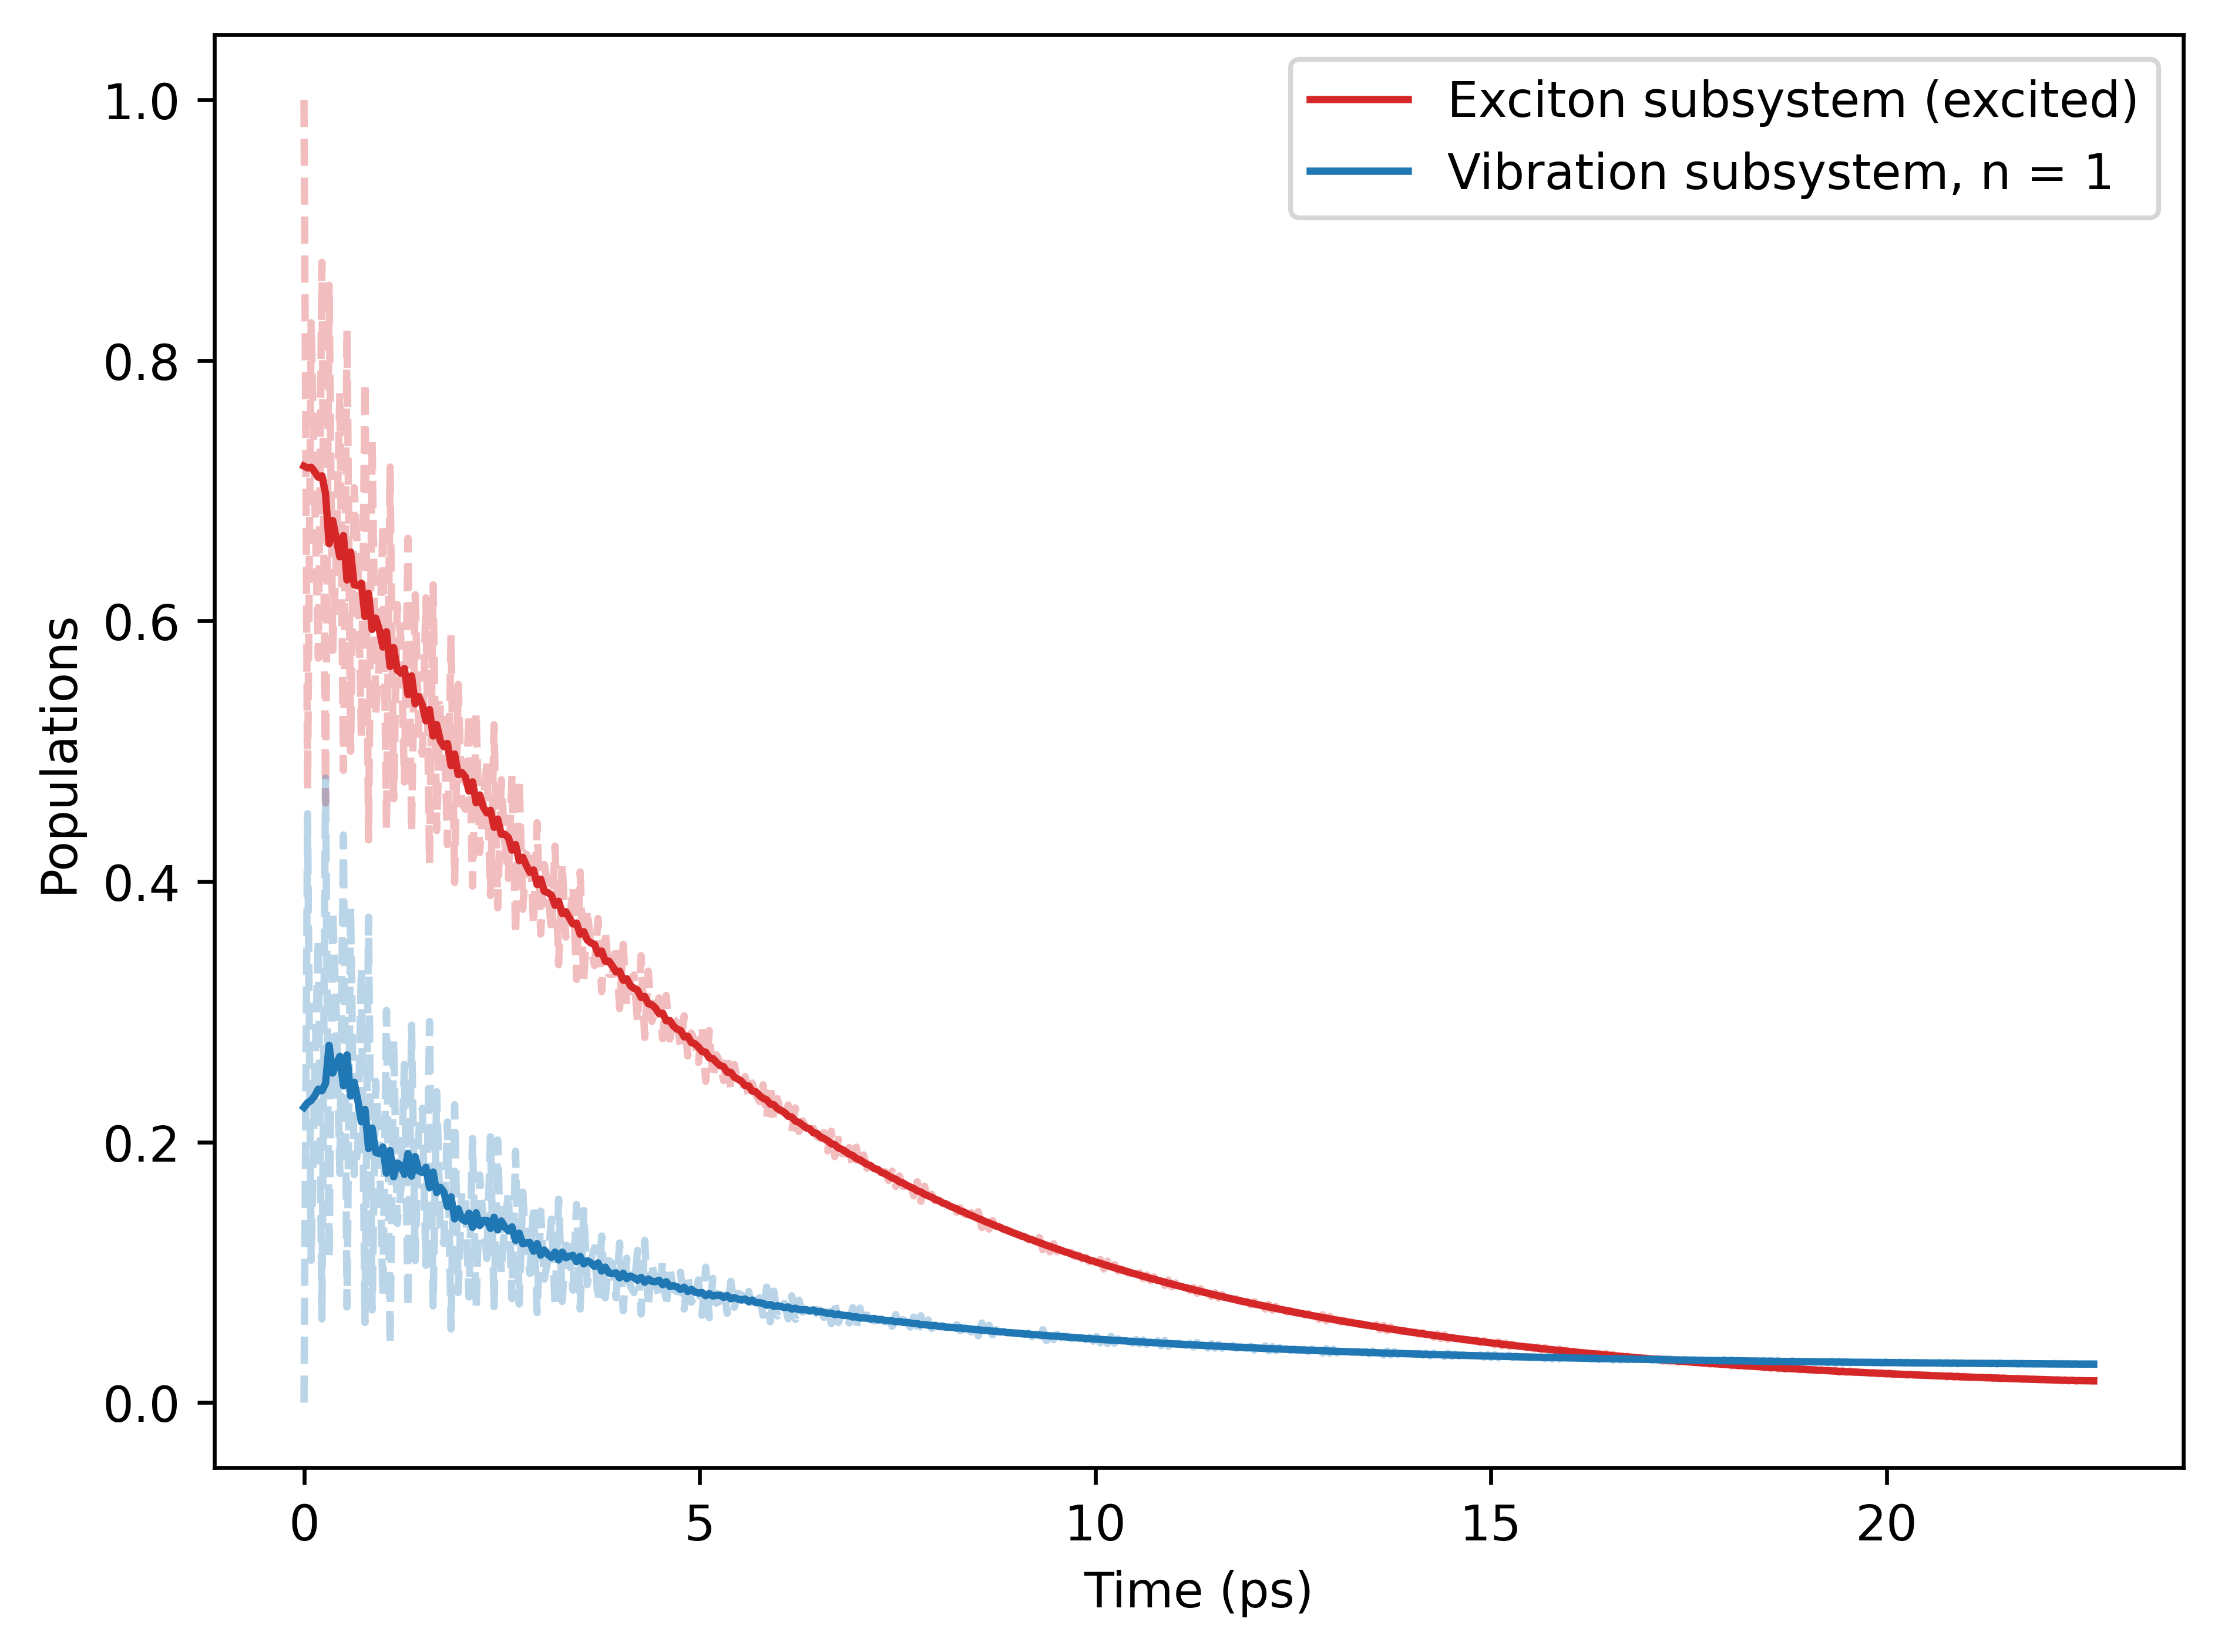
\includegraphics[width=0.49\textwidth]{Research Project/Code/results/ExVib/Open/Population/Envelope/pops_ex_therm_e0.png}
        \hfill
        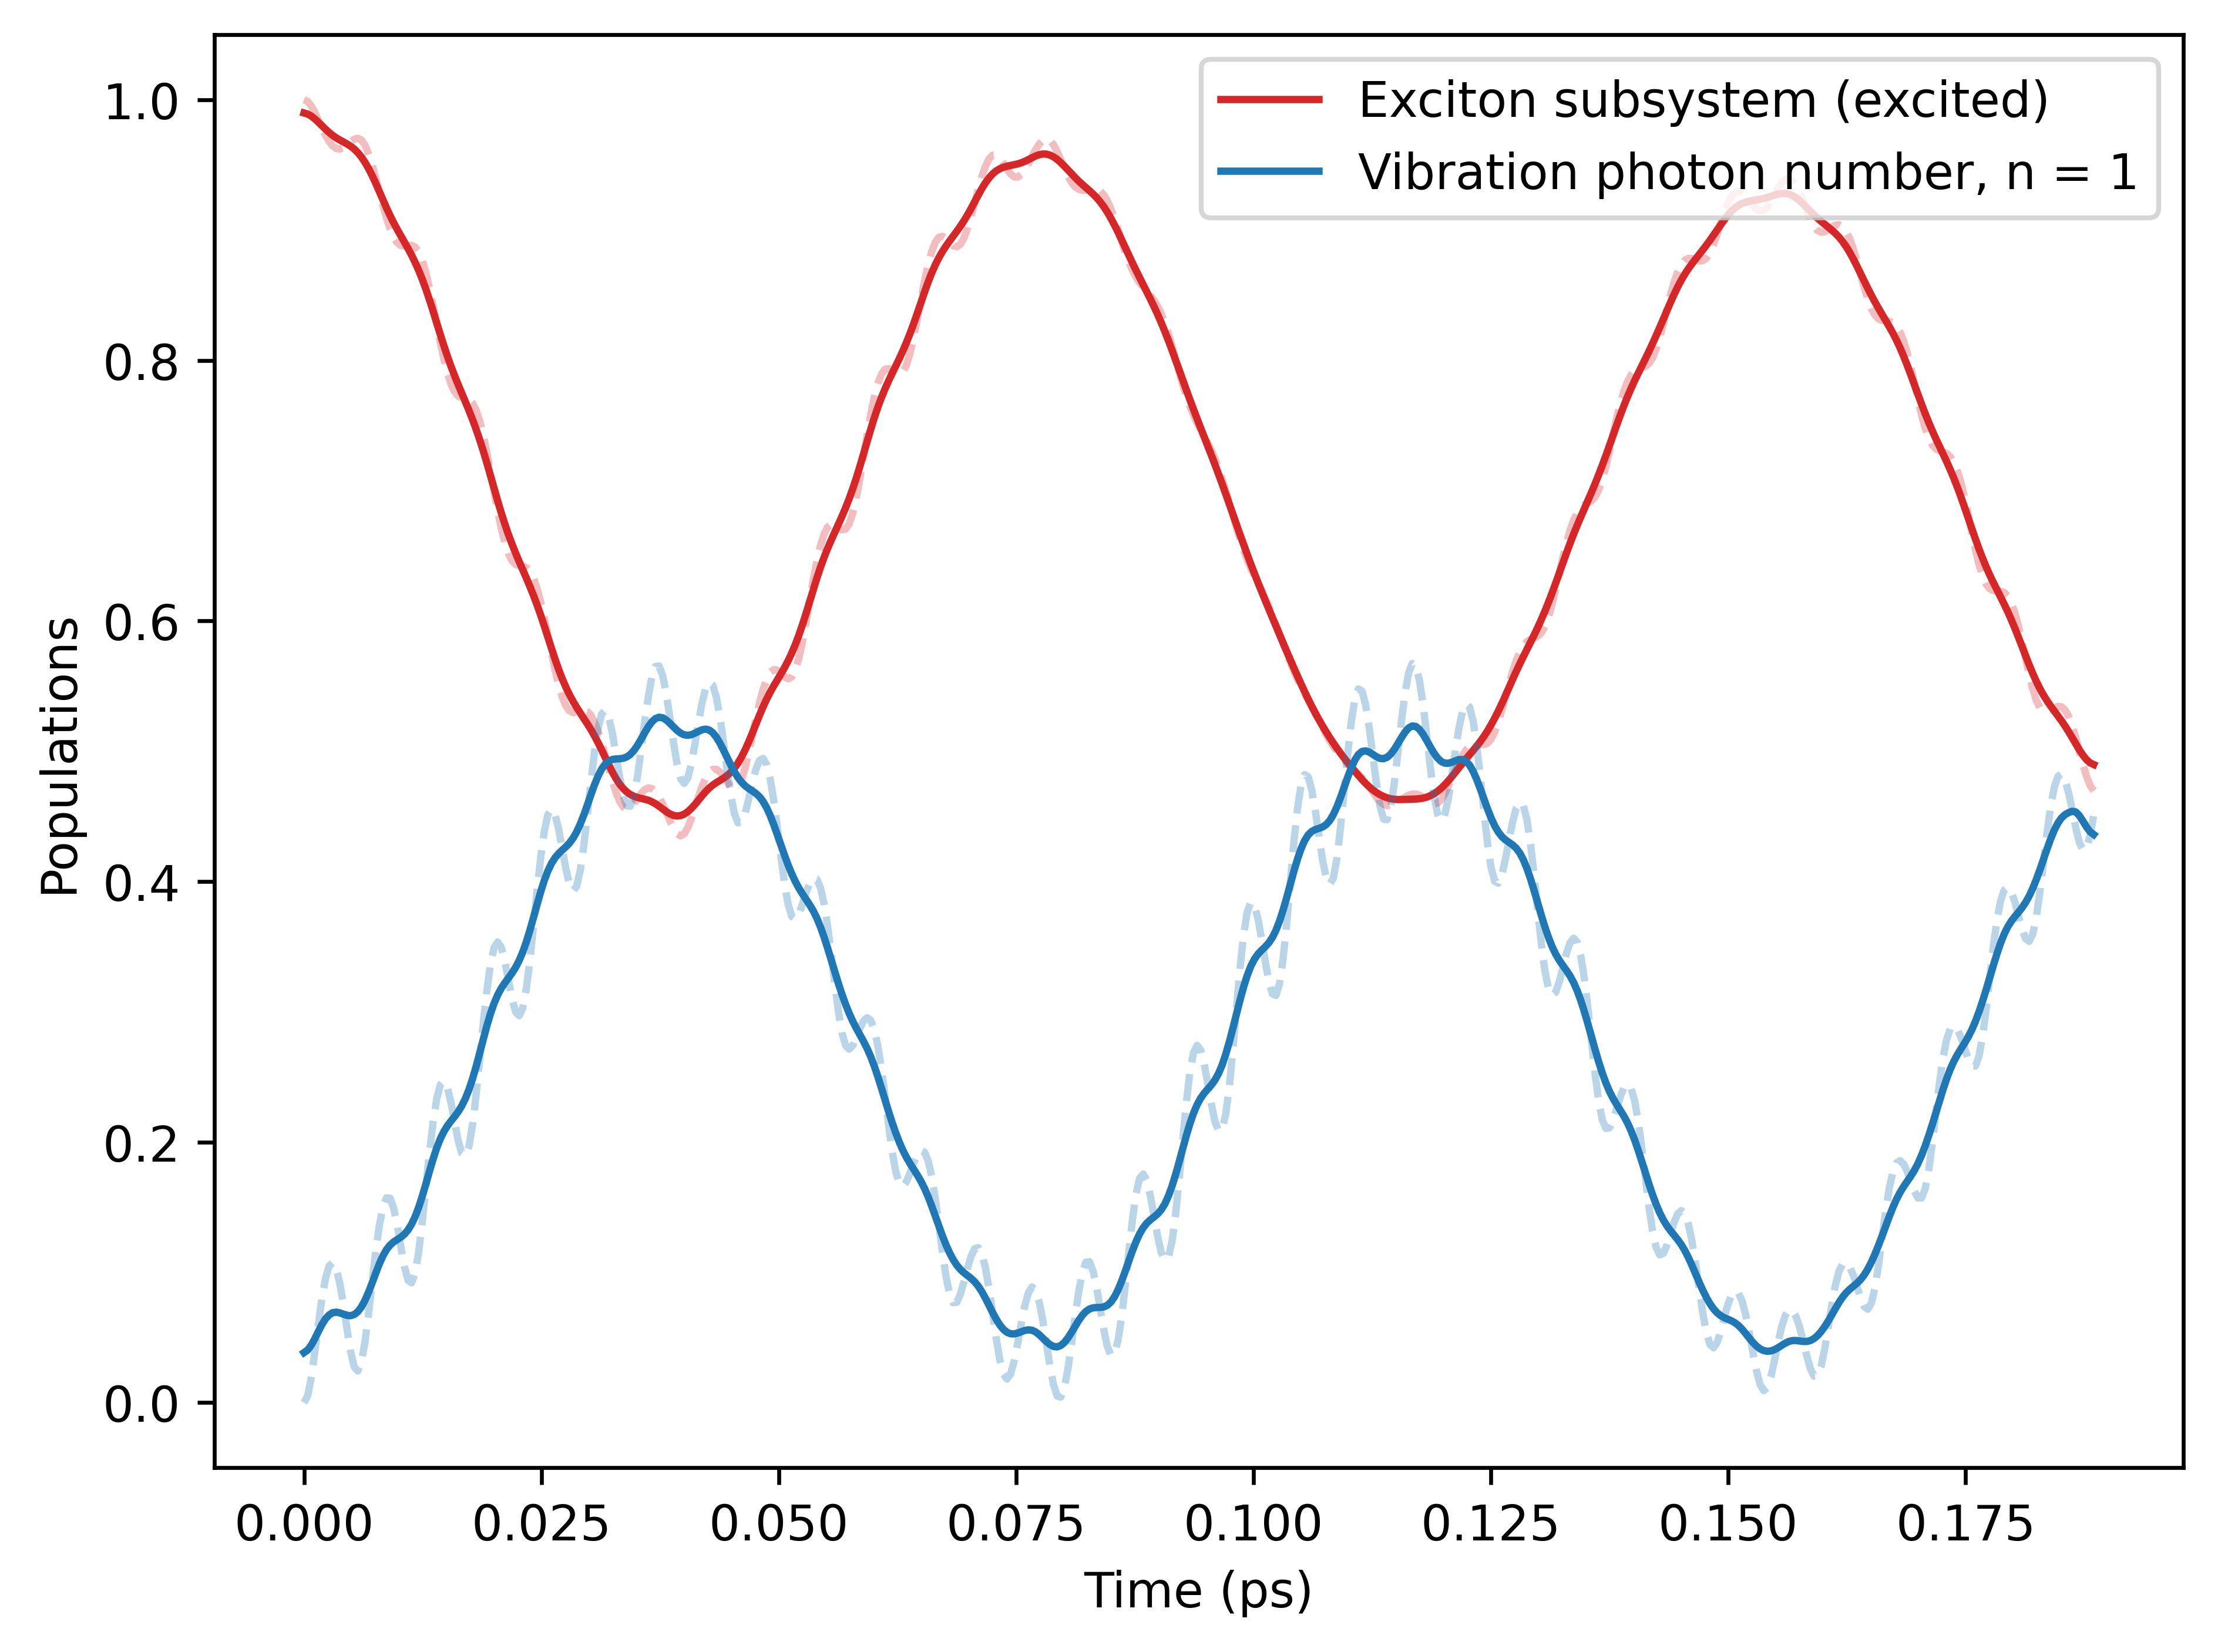
\includegraphics[width=0.49\textwidth]{Research Project/Code/results/ExVib/Open/Population/Fast/pops_ex_therm_e0.png}
        \caption{}
        \label{fig:EVM_OQS_Pop_therm_e0}
    \end{subfigure}

    \vspace{0.8em}

    % -------- Row (c): Both channels --------
    \begin{subfigure}{\textwidth}
        \centering
        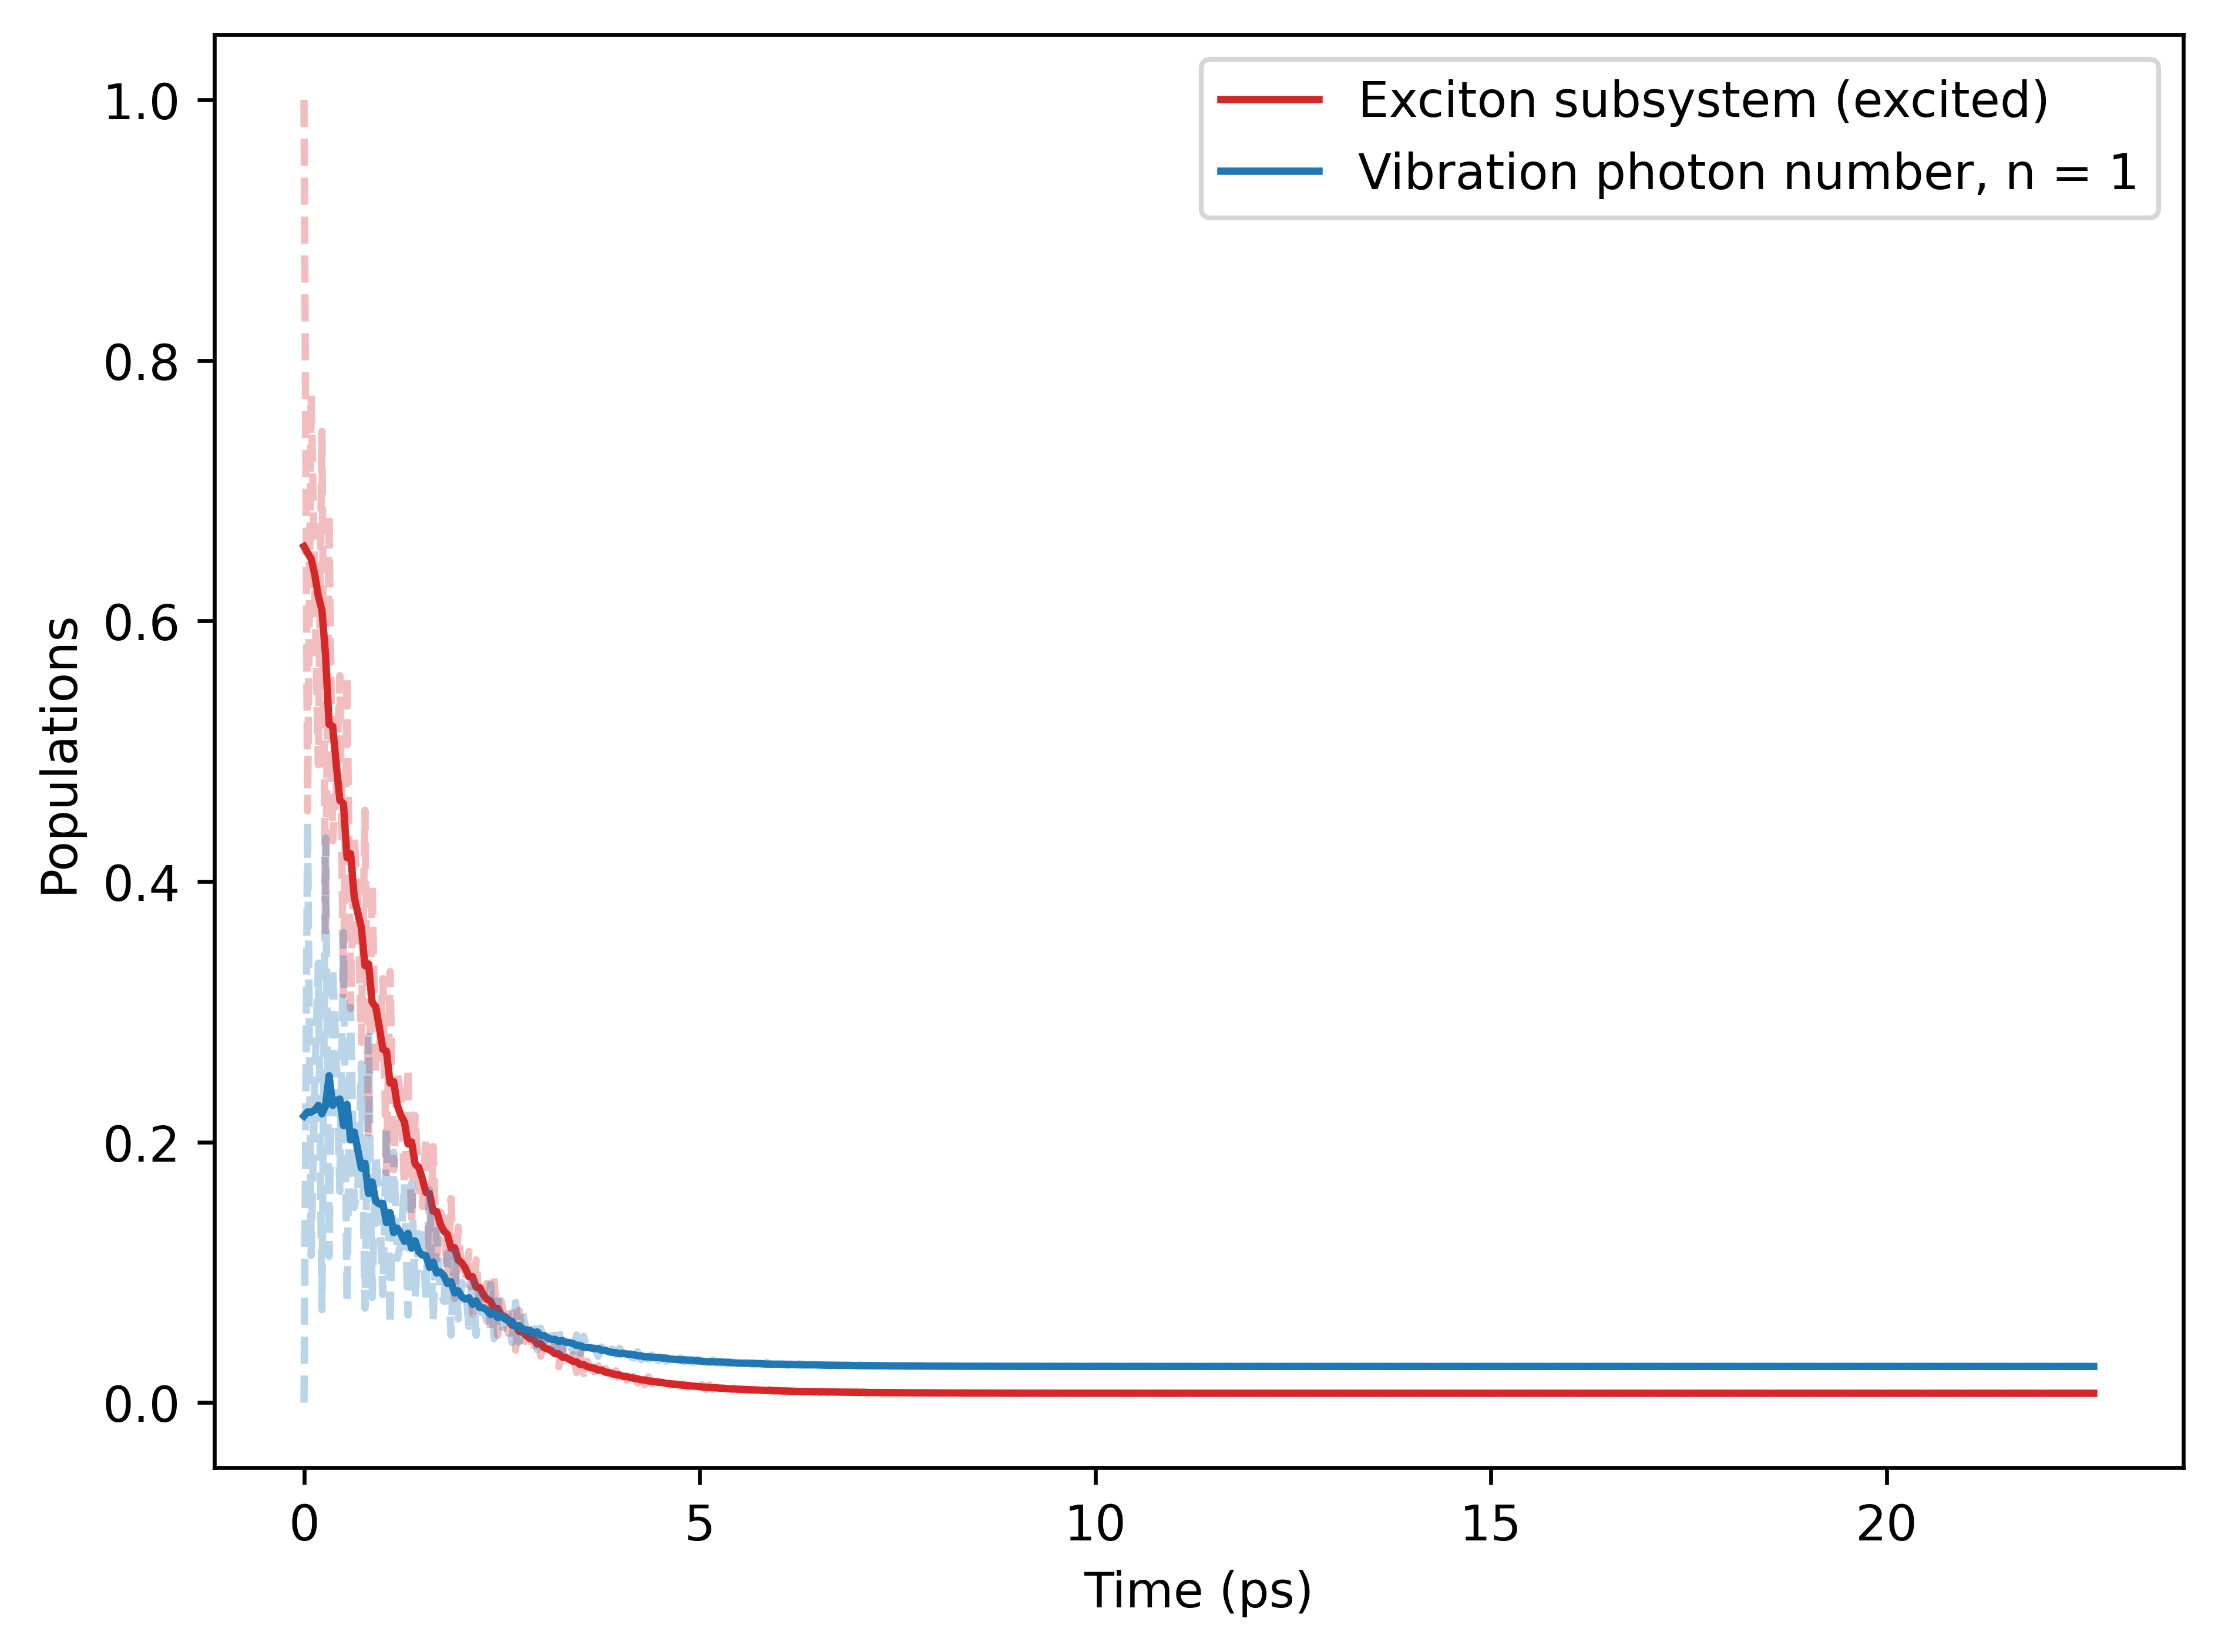
\includegraphics[width=0.49\textwidth]{Research Project/Code/results/ExVib/Open/Population/Envelope/pops_ex_both_e0.png}
        \hfill
        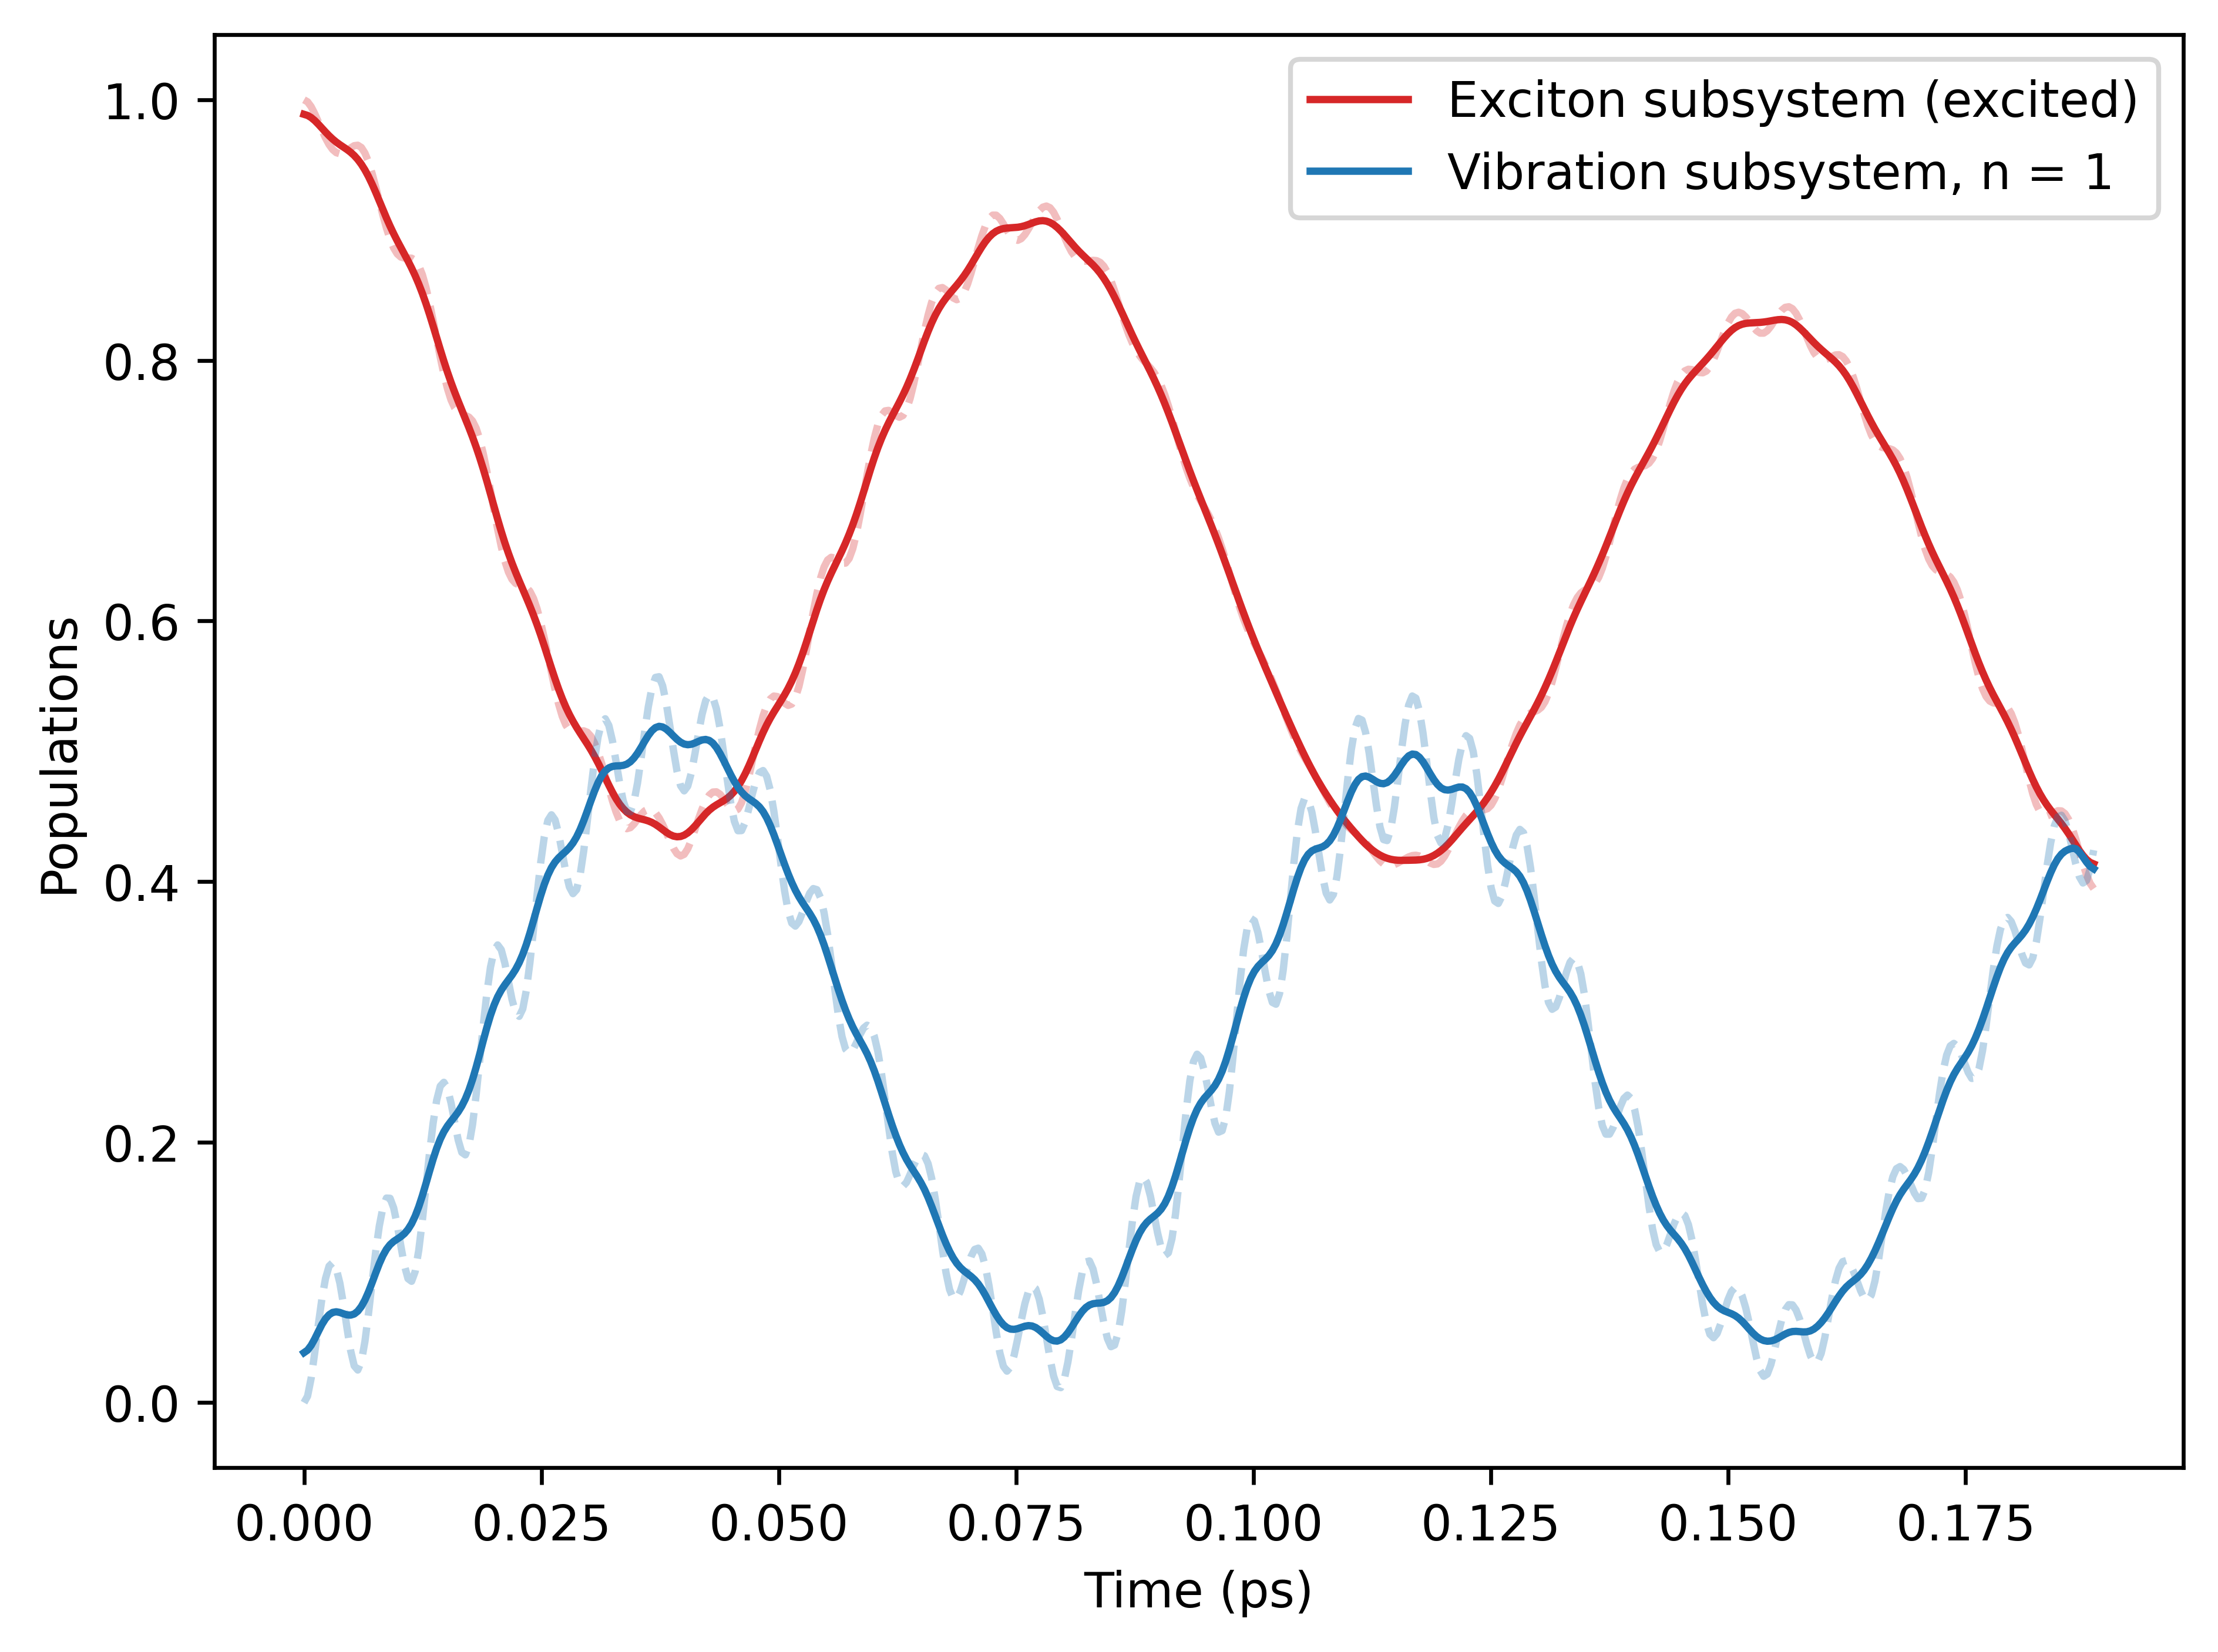
\includegraphics[width=0.49\textwidth]{Research Project/Code/results/ExVib/Open/Population/Fast/pops_ex_both_e0.png}
        \caption{}
        \label{fig:EVM_OQS_Pop_both_e0}
    \end{subfigure}
    \caption{Plots of the EVM subsystem populations under open system evolution, with an initial state of $|\psi (\text{t=0})\rangle = |1, 0\rangle$. The left--hand column of sub--figures is plotted over a long picosecond timescale to demonstrate envelope and medium frequency oscillations, as well as overall decay. The right--hand column of sub--figures is plotted over a shorter timescale to demonstrate high frequency oscillations. (a) Evolution under spontaneous atomic emission. (b) Evolution under thermal dissipation. (c) Evolution under both spontaneous atomic emission and thermal dissipation.}
    \label{fig:EVM_OQS_Pop_e0}
\end{figure}
\vspace{-0.1cm}
\noindent more pronounced population transfer between excitonic states, and so our rates of decay would be nearer in value.
When both decay channels are open simultaneously (Figure \ref{fig:EVM_OQS_Pop_both_e0}), both subsystems decay much faster than when their corresponding decay operators were acting in isolation. Both the exciton and vibration subsystem decay to a steady state at $\approx 6$ps. While the exciton decays to its ground state, the vibrational mode decays to a steady state that is not its ground state of $|n=0\rangle$. We may attribute this to the thermal dissipation channel having a high enough value of $k_bT = 208.5\text{ cm}^{-1}$ that the mean thermal occupation number N (see equation \eqref{eqn:H_EV}) is non--zero, and thus there is a finite temperature bath. In this scenario, there always remains a small equilibrium population in the vibration, so it never decays fully to its ground state.\\
\\
This finite temperature bath regime becomes more apparent when we analyse the entanglement of our system, quantified by negativity measure (Figure \ref{fig:EVM_OQS_Neg_e0}). As expected, the initial entanglement decays rapidly under spontaneous atomic emission (Figure \ref{fig:EVM_OQS_Neg_spont_e0}). In contrast, the thermal dissipation channel takes longer to decay (Figure \ref{fig:EVM_OQS_Neg_therm_e0}). The Lindblad operators cause both collapse and revive populations of the vibration subsystem, such that the oscillator is continually driven from its ground state. The exicton--exciton coupling term does not decay, and so both excited and ground exciton states remain. Both effects in unison cause non--classical correlations between the exciton and vibration, giving rise to small but persistent steady--state entanglement. When both decay channels are active simultaneously, decay is faster overall, but again, the finite--temperature bath gives rise to excitations in the vibration subsystem, and a similar residual entanglement is observed. Surprisingly, under spontaneous atomic emission, where there are no revival mechanisms for either subsystem, entanglement seems to increase, suggesting the presence of a minimum. This could perhaps be explained by numerical instability in our QuTip solver methods.\\
\\
A similar picture emerges when analysing coherence, quantified using the relative entropy of coherence (Figure \ref{fig:EVM_OQS_Coh_e0}). For all plots, we observe that the coherence in the subsystems are initially non--zero and gradually decay, consistent with our observations for the closed evolution. Under spontaneous emission (Figure \ref{fig:EVM_OQS_Coh_spont_e0}), the system is expected to relax to the separable ground state with vanishing coherence. However, as with entanglement, our simulations display a residual coherence. The origin of this effect is not entirely clear: it may rise from numerical artefacts, or be linked to the interaction Hamiltonian of the EVM. We are unable to conclusively determine which mechanism is responsible for this effect, and we associate it with a limitation of the simulation. In contrast, the behaviour under thermal dissipation is well understood. The channel sustains a stable level of coherence in the vibration subsystem (around $\approx 0.18$) due to the finite-temperature bath. The coherence of the exciton subsystem under this decay channel is expected to be weak, and we observe this. The interaction Hamiltonian couples these vibrational excitations to the exciton via the displacement term $\sigma_z(b^\dagger+b)$, while the $V\sigma_x$ term ensures that the TLS does not remain strictly diagonal in the $\{{|0\rangle,|1\rangle}\}$ basis. As a result, the joint density matrix retains weak but persistent off--diagonal elements that survive into the steady state. We further observe that when both decay channels are present (Figure \ref{fig:EVM_OQS_Coh_both_e0}), exciton coherence is quickly suppressed by spontaneous emission, but the vibrational subsystem continues to sustain a small degree of coherence due to the thermal bath. This residual vibrational contribution ensures that the total system retains a non–zero baseline of coherence at long times.

%%%%%% NEG %%%%%%%%%%%%%%%%%
\begin{figure}[H]
    \centering
    % -------- Row (a): Spontaneous emission --------
    \begin{subfigure}{\textwidth}
        \centering
        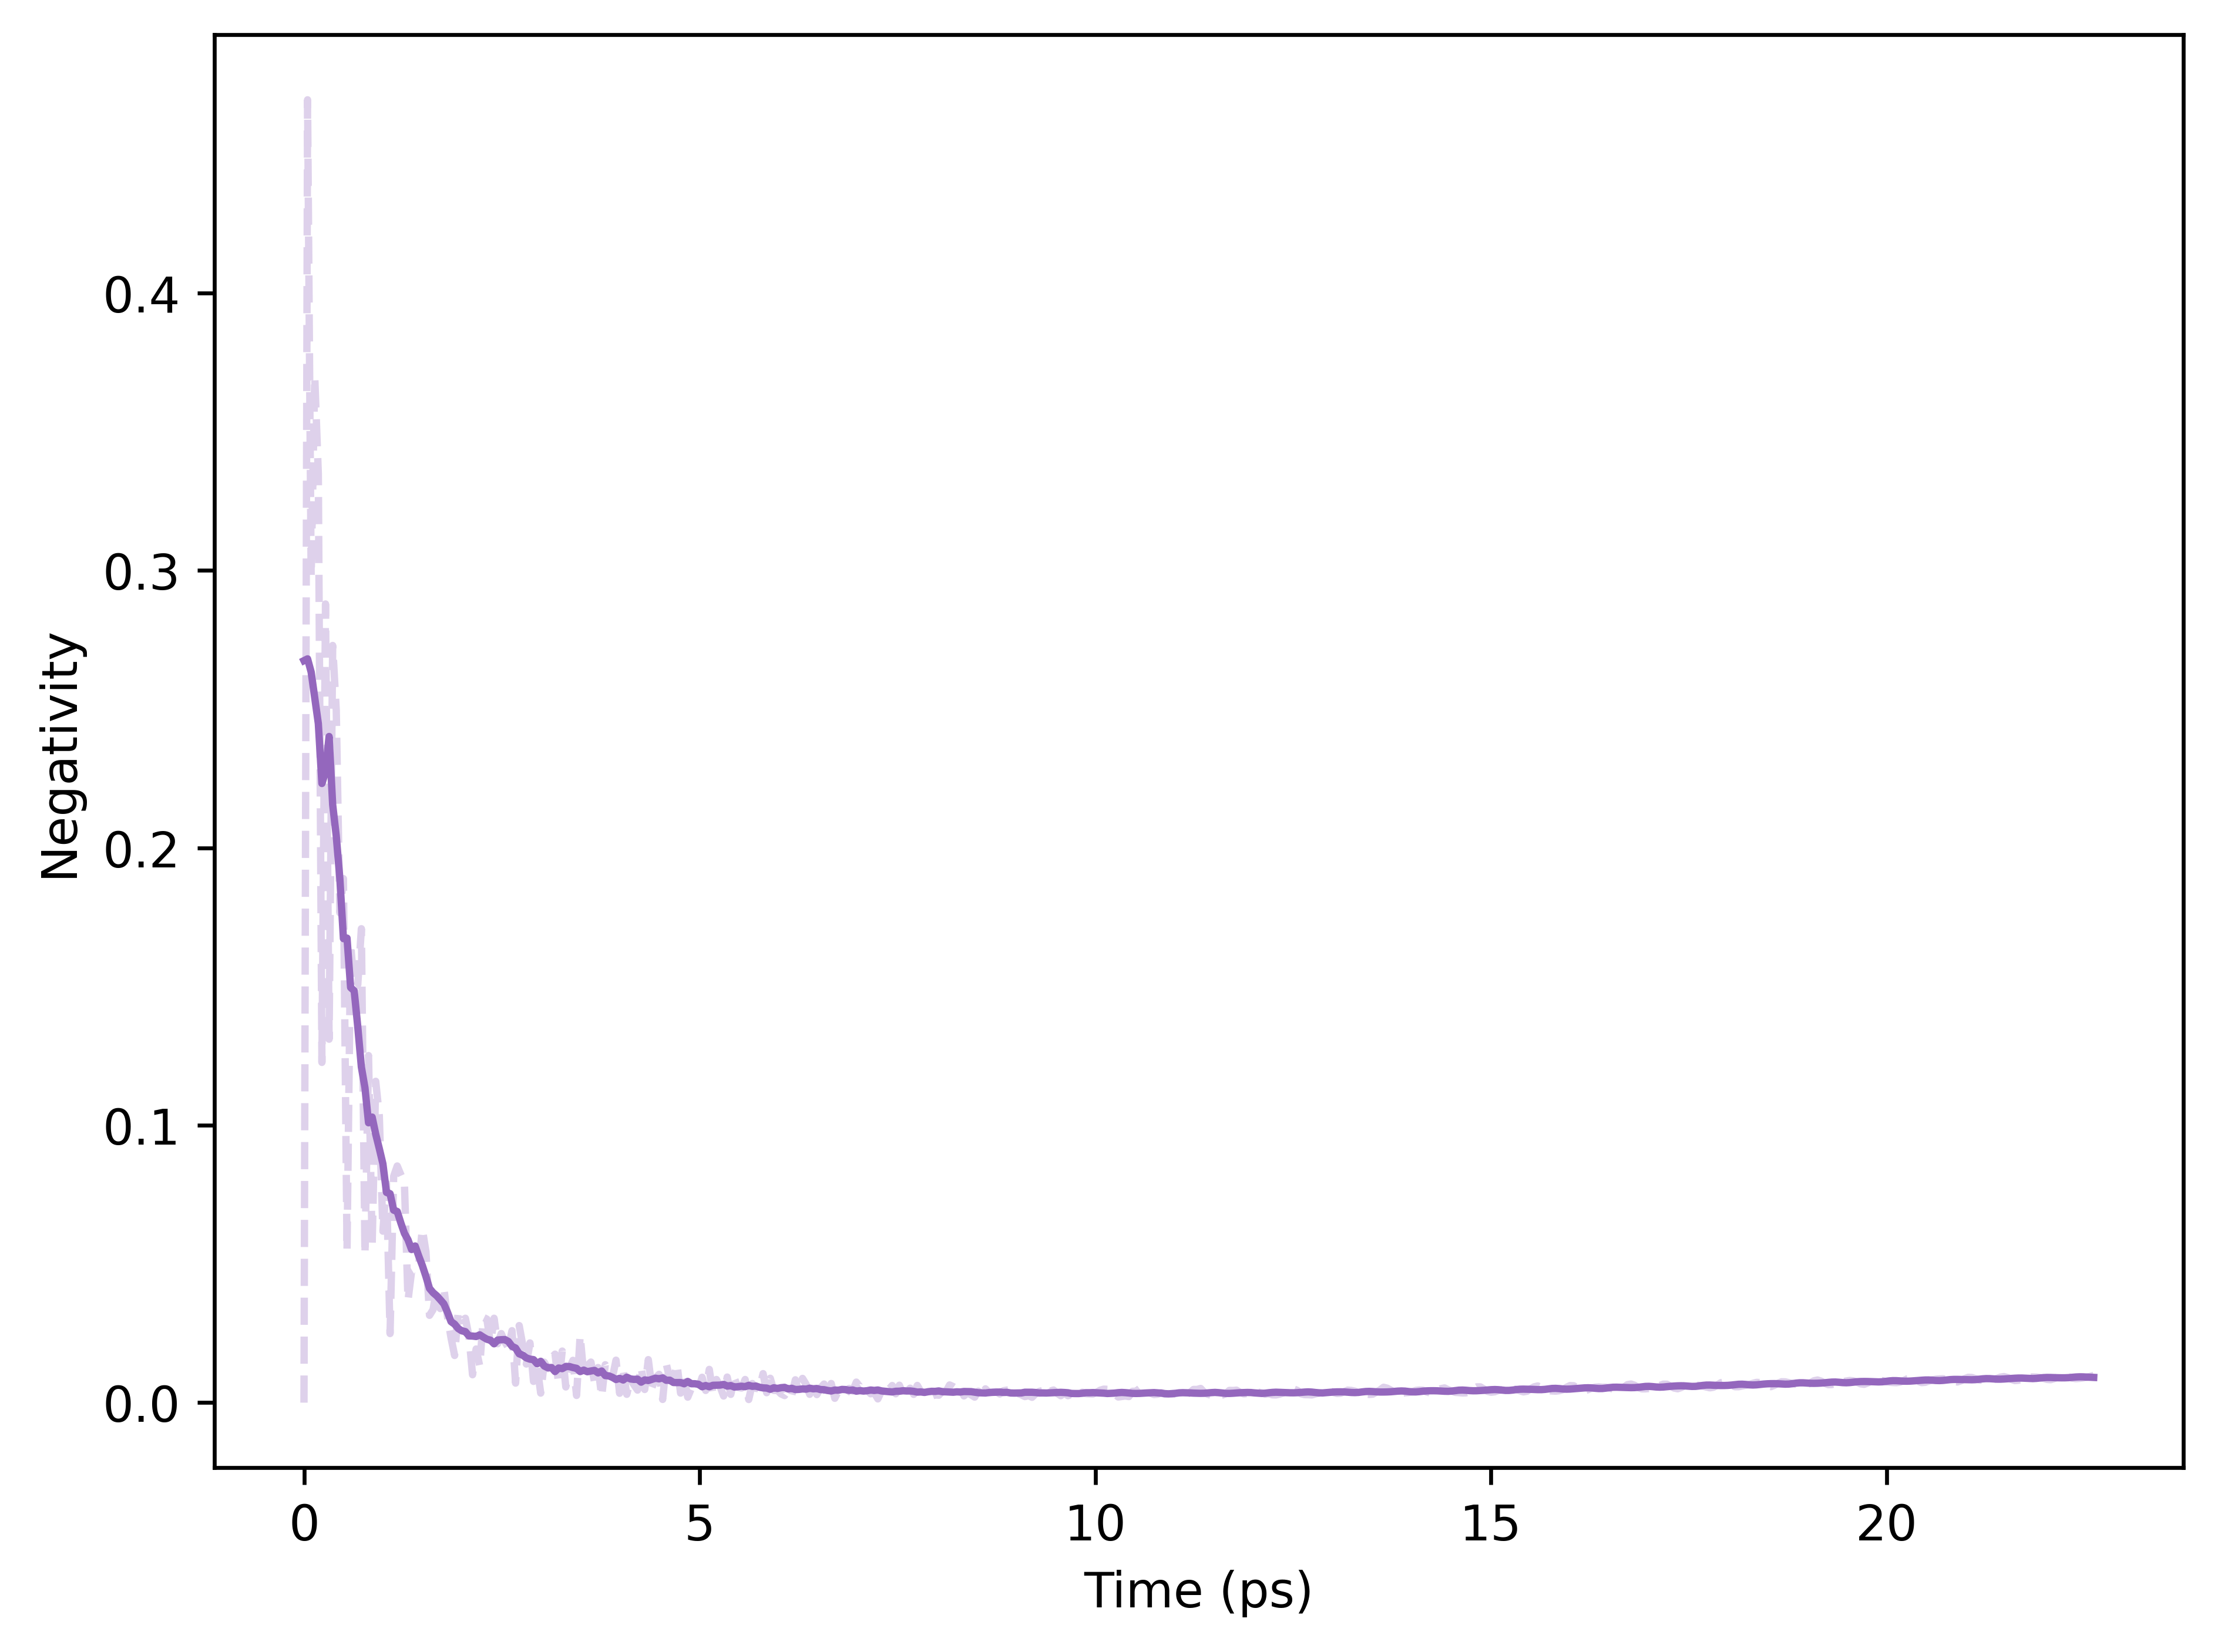
\includegraphics[width=0.49\textwidth]{Research Project/Code/results/ExVib/Open/Negativity/Envelope/neg_spont_e0.png}
        \hfill
        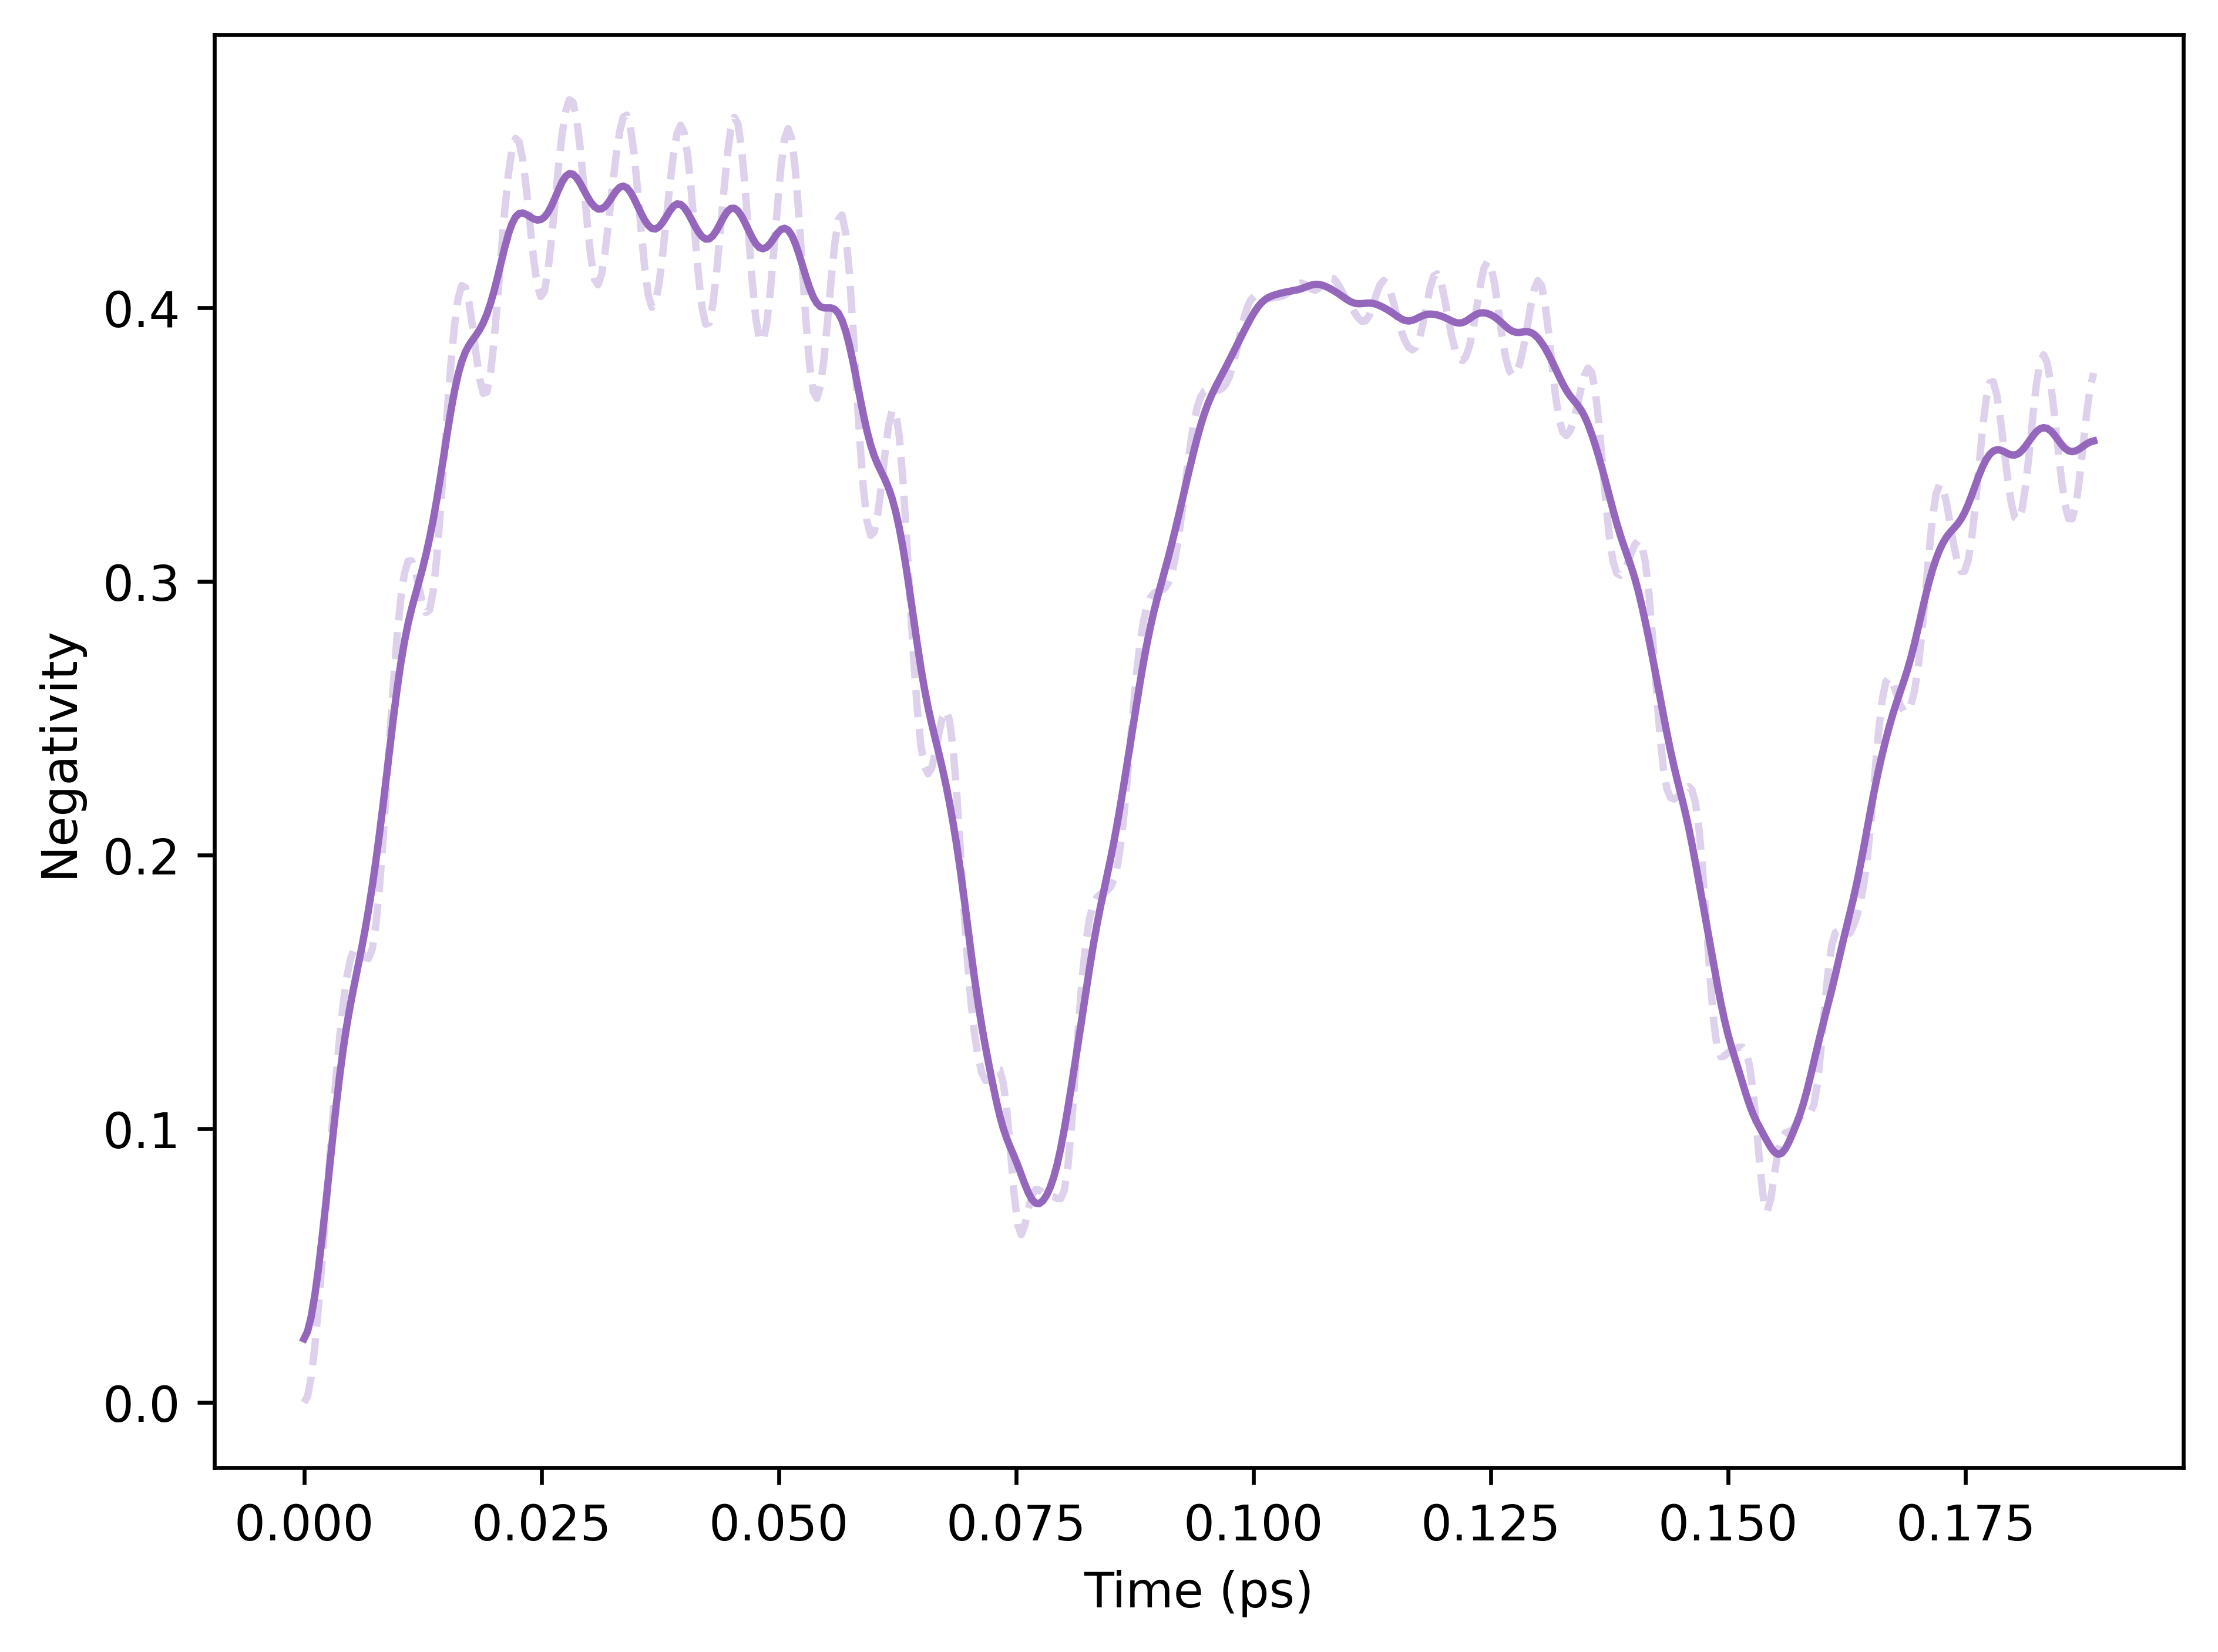
\includegraphics[width=0.49\textwidth]{Research Project/Code/results/ExVib/Open/Negativity/Fast/neg_spont_e0.png}
        \caption{}
        \label{fig:EVM_OQS_Neg_spont_e0}
    \end{subfigure}

    \vspace{0.8em}

    % -------- Row (b): Thermal dissipation --------
    \begin{subfigure}{\textwidth}
        \centering
        \includegraphics[width=0.49\textwidth]{Research Project/Code/results/ExVib/Open/Negativity/Envelope/neg_therm_e0.png}
        \hfill
        \includegraphics[width=0.49\textwidth]{Research Project/Code/results/ExVib/Open/Negativity/Fast/neg_therm_e0.png}
        \caption{}
        \label{fig:EVM_OQS_Neg_therm_e0}
    \end{subfigure}

    \vspace{0.8em}

    % -------- Row (c): Both channels --------
    \begin{subfigure}{\textwidth}
        \centering
        \includegraphics[width=0.49\textwidth]{Research Project/Code/results/ExVib/Open/Negativity/Envelope/neg_both_e0.png}
        \hfill
        \includegraphics[width=0.49\textwidth]{Research Project/Code/results/ExVib/Open/Negativity/Fast/neg_both_e0.png}
        \caption{}
        \label{fig:EVM_OQS_Neg_both_e0}
    \end{subfigure}
    \caption{Plots of the decay of entanglement of the EVM under open system evolution using the negativity measure, with an initial state of $|\psi (\text{t=0})\rangle = |1, 0\rangle$. The left--hand column of sub--figures is plotted over a long picosecond timescale to demonstrate envelope and medium frequency oscillations, as well as overall decay. The right--hand column of sub--figures is plotted over a shorter timescale to demonstrate high frequency oscillations. (a) Entanglement decay under spontaneous atomic emission. (b) Entanglement decay under thermal dissipation. (c) Entanglement decay under both spontaneous atomic emission and thermal dissipation.}
    \label{fig:EVM_OQS_Neg_e0}
\end{figure}


%%%%%%%% COH %%%%%%%%%
\begin{figure}[H]
    \centering

    % -------- Row (a): Spontaneous emission --------
    \begin{subfigure}{\textwidth}
        \centering
        \includegraphics[width=0.49\textwidth]{Research Project/Code/results/ExVib/Open/Coherence/Envelope/coh_spont_e0.png}
        \hfill
        \includegraphics[width=0.49\textwidth]{Research Project/Code/results/ExVib/Open/Coherence/Fast/coh_spont_e0.png}
        \caption{}
        \label{fig:EVM_OQS_Coh_spont_e0}
    \end{subfigure}

    \vspace{0.8em}

    % -------- Row (b): Thermal dissipation --------
    \begin{subfigure}{\textwidth}
        \centering
        \includegraphics[width=0.49\textwidth]{Research Project/Code/results/ExVib/Open/Coherence/Envelope/coh_therm_e0.png}
        \hfill
        \includegraphics[width=0.49\textwidth]{Research Project/Code/results/ExVib/Open/Coherence/Fast/coh_therm_e0.png}
        \caption{}
        \label{fig:EVM_OQS_Coh_therm_e0}
    \end{subfigure}

    \vspace{0.8em}

    % -------- Row (c): Both channels --------
    \begin{subfigure}{\textwidth}
        \centering
        \includegraphics[width=0.49\textwidth]{Research Project/Code/results/ExVib/Open/Coherence/Envelope/coh_both_e0.png}
        \hfill
        \includegraphics[width=0.49\textwidth]{Research Project/Code/results/ExVib/Open/Coherence/Fast/coh_both_e0.png}
        \caption{}
        \label{fig:EVM_OQS_Coh_both_e0}
    \end{subfigure}
    \caption{Plots of the decay of coherence (decoherence) of the EVM under open system evolution using the relative entropy of coherence measure, with an initial state of $|\psi (\text{t=0})\rangle =|1, 0\rangle$. The left--hand column of sub--figures is plotted over a long picosecond timescale to demonstrate envelope and medium frequency oscillations, as well as overall decay. The right--hand column of sub--figures is plotted over a shorter timescale to demonstrate high frequency oscillations. (a) Decoherence under spontaneous atomic emission. (b) Decoherence under thermal dissipation. (c) Decoherence under both spontaneous atomic emission and thermal dissipation.}
    \label{fig:EVM_OQS_Coh_e0}
\end{figure}

%%%%%%%%%%%%%%%%%%%%%%%% EVM OQS II %%%%%%%%%%%%%%%%%%%%%

%%%%%%%% POPS %%%%%%%%
\subsubsubsection{Case II: Superposition Initial Condition}

As with the closed simulation, we also consider the second initial state in equation \eqref{eqn:init_EVM_e0g0}.
\begin{figure}[H]
    \centering

    % -------- Row (a): Spontaneous emission --------
    \begin{subfigure}{\textwidth}
        \centering
        \includegraphics[width=0.49\textwidth]{Research Project/Code/results/ExVib/Open/Population/Envelope/pops_ex_spont_eg.png}
        \hfill
        \includegraphics[width=0.49\textwidth]{Research Project/Code/results/ExVib/Open/Population/Fast/pops_ex_spont_eg.png}
        \caption{}
        \label{fig:EVM_OQS_Pop_spont_eg}
    \end{subfigure}

    \vspace{0.8em}

    % -------- Row (b): Thermal dissipation --------
    \begin{subfigure}{\textwidth}
        \centering
        \includegraphics[width=0.49\textwidth]{Research Project/Code/results/ExVib/Open/Population/Envelope/pops_ex_therm_eg.png}
        \hfill
        \includegraphics[width=0.49\textwidth]{Research Project/Code/results/ExVib/Open/Population/Fast/pops_ex_therm_eg.png}
        \caption{}
        \label{fig:EVM_OQS_Pop_therm_eg}
    \end{subfigure}

    \vspace{0.8em}

    % -------- Row (c): Both channels --------
    \begin{subfigure}{\textwidth}
        \centering
        \includegraphics[width=0.49\textwidth]{Research Project/Code/results/ExVib/Open/Population/Envelope/pops_ex_both_eg.png}
        \hfill
        \includegraphics[width=0.49\textwidth]{Research Project/Code/results/ExVib/Open/Population/Fast/pops_ex_both_eg.png}
        \caption{}
        \label{fig:EVM_OQS_Pop_both_eg}
    \end{subfigure}
    \caption{Plots of the EVM subsystem populations under open system evolution, with an initial state of $|\psi (\text{t=0})\rangle = 1/\sqrt{2}(|1\rangle + |0\rangle)\otimes|n=0\rangle$. The left--hand column of sub--figures is plotted over a long picosecond timescale to demonstrate envelope and medium frequency oscillations, as well as overall decay. The right--hand column of sub--figures is plotted over a shorter timescale to demonstrate high frequency oscillations. (a) Evolution under spontaneous atomic emission. (b) Evolution under thermal dissipation. (c) Evolution under both spontaneous atomic emission and thermal dissipation.}
    \label{fig:EVM_OQS_Pop_eg}
\end{figure}

The populations of both subsystems in Figure \ref{fig:EVM_OQS_Pop_eg} exhibit similar patterns to those of the first initial state. When the spontaneous atomic emission channel is open (Figure \ref{fig:EVM_OQS_Pop_spont_eg}), the exciton subsystem decays in roughly $10$ ps, matching our previous case; the same follows for our vibration subsystem. When only the thermal dissipation channel is active (Figure \ref{fig:EVM_OQS_Pop_therm_eg}), we observe similar exciton subsystem decay rates in the populations; the vibration subsystem also decays, but exhibits the steady--state feature observed earlier. With both channels active (Figure \ref{fig:EVM_OQS_Pop_both_eg}), both subsystems decay more rapidly, as expected, due to the finite--temperature bath and interaction coupling between both subsystems. An interesting feature of all three decay models, however, is that the medium oscillations are much stronger. This suggests that the coupling strength between the subsystems, $g$, is preserved for a longer time. We may therefore conclude that starting in an excitonic superposition state makes the exciton--vibration exchange processes more pronounced..\\
\\
The entanglement of the total system (Figure \ref{fig:EVM_OQS_Neg_eg}) exhibits similar behaviours to our previous initial condition. Overall entanglement is reduced due to the dilution introduced by stationary states. The decay timescales for all three decay channels remain comparable to those of the previous case. The main distinction is that the medium--frequency oscillations are more pronounced, consistent with the population dynamics. Thus, while the maximum achievable entanglement is reduced, the stronger medium--frequency oscillations remain distinct throughout evolution. \\
\\
Lastly, we observe similar decay timescales and steady--state coherence in Figure \ref{fig:EVM_OQS_Coh_eg}, as with the previous initial condition. A characteristic feature of the current initial state, as noted in Section \ref{EVM_CQS_case2}, is that the exciton subsystem becomes a stronger carrier of coherence across all decay types, owing to the  superposition in the initial state. Again, the medium--frequency oscillations are pronounced, but they do not have a particular effect on the decay timescales. We also note that, whereas under closed evolution the coherences of both the subsystems and total systems are stronger, here it seems that decoherence rapidly suppresses them (within less than $1$ ps), diminishing the effectiveness of this initial condition in sustaining stronger coherence, and thus reducing the advantage of this initial state in the generation of coherence.\\
\\
This concludes our analysis of the EVM under both closed and open evolution of the system. We now turn to discuss both models, summarising their unique features of entanglement and coherence, and comparing their strengths and weaknesses. 

%%%%%%%% NEG %%%%%%%%%
\begin{figure}[H]
    \centering
    % -------- Row (a): Spontaneous emission --------
    \begin{subfigure}{\textwidth}
        \centering
        \includegraphics[width=0.49\textwidth]{Research Project/Code/results/ExVib/Open/Negativity/Envelope/neg_spont_eg.png}
        \hfill
        \includegraphics[width=0.49\textwidth]{Research Project/Code/results/ExVib/Open/Negativity/Fast/neg_spont_eg.png}
        \caption{}
        \label{fig:EVM_OQS_Neg_spont_eg}
    \end{subfigure}

    \vspace{0.8em}

    % -------- Row (b): Thermal dissipation --------
    \begin{subfigure}{\textwidth}
        \centering
        \includegraphics[width=0.49\textwidth]{Research Project/Code/results/ExVib/Open/Negativity/Envelope/neg_therm_eg.png}
        \hfill
        \includegraphics[width=0.49\textwidth]{Research Project/Code/results/ExVib/Open/Negativity/Fast/neg_therm_eg.png}
        \caption{}
        \label{fig:EVM_OQS_Neg_therm_eg}
    \end{subfigure}

    \vspace{0.8em}

    % -------- Row (c): Both channels --------
    \begin{subfigure}{\textwidth}
        \centering
        \includegraphics[width=0.49\textwidth]{Research Project/Code/results/ExVib/Open/Negativity/Envelope/neg_both_eg.png}
        \hfill
        \includegraphics[width=0.49\textwidth]{Research Project/Code/results/ExVib/Open/Negativity/Fast/neg_both_eg.png}
        \caption{}
        \label{fig:EVM_OQS_Neg_both_eg}
    \end{subfigure}
    \caption{Plots of the decay of entanglement of the EVM under open system evolution using the negativity measure, with an initial state of $|\psi (\text{t=0})\rangle = 1/\sqrt{2}(|1\rangle + |0\rangle)\otimes|n=0\rangle$. The left--hand column of sub--figures is plotted over a long picosecond timescale to demonstrate envelope and medium frequency oscillations, as well as overall decay. The right--hand column of sub--figures is plotted over a shorter timescale to demonstrate high frequency oscillations. (a) Entanglement decay under spontaneous atomic emission. (b) Entanglement decay under thermal dissipation. (c) Entanglement decay under both spontaneous atomic emission and thermal dissipation.}
    \label{fig:EVM_OQS_Neg_eg}
\end{figure}


%%%%%%%% COH %%%%%%%%%%%%
\begin{figure}[H]
    \centering

    % -------- Row (a): Spontaneous emission --------
    \begin{subfigure}{\textwidth}
        \centering
        \includegraphics[width=0.49\textwidth]{Research Project/Code/results/ExVib/Open/Coherence/Envelope/coh_spont_eg.png}
        \hfill
        \includegraphics[width=0.49\textwidth]{Research Project/Code/results/ExVib/Open/Coherence/Fast/coh_spont_eg.png}
        \caption{}
        \label{fig:EVM_OQS_Coh_spont_eg}
    \end{subfigure}

    \vspace{0.8em}

    % -------- Row (b): Thermal dissipation --------
    \begin{subfigure}{\textwidth}
        \centering
        \includegraphics[width=0.49\textwidth]{Research Project/Code/results/ExVib/Open/Coherence/Envelope/coh_therm_eg.png}
        \hfill
        \includegraphics[width=0.49\textwidth]{Research Project/Code/results/ExVib/Open/Coherence/Fast/coh_therm_eg.png}
        \caption{}
        \label{fig:EVM_OQS_Coh_therm_eg}
    \end{subfigure}

    \vspace{0.8em}

    % -------- Row (c): Both channels --------
    \begin{subfigure}{\textwidth}
        \centering
        \includegraphics[width=0.49\textwidth]{Research Project/Code/results/ExVib/Open/Coherence/Envelope/coh_both_eg.png}
        \hfill
        \includegraphics[width=0.49\textwidth]{Research Project/Code/results/ExVib/Open/Coherence/Fast/coh_both_eg.png}
        \caption{}
        \label{fig:EVM_OQS_Coh_both_eg}
    \end{subfigure}
    \caption{Plots of the decay of coherence (decoherence) of the EVM under open system evolution using the relative entropy of coherence measure, with an initial state of $|\psi (\text{t=0})\rangle = 1/\sqrt{2}(|1\rangle + |0\rangle)\otimes|n=0\rangle$. The left--hand column of sub--figures is plotted over a long picosecond timescale to demonstrate envelope and medium frequency oscillations, as well as overall decay. The right--hand column of sub--figures is plotted over a shorter timescale to demonstrate high frequency oscillations. (a) Decoherence under spontaneous atomic emission. (b) Decoherence under thermal dissipation. (c) Decoherence under both spontaneous atomic emission and thermal dissipation.}
    \label{fig:EVM_OQS_Coh_eg}
\end{figure}
%%%%%%%%%%%%%%%%%%%%%%%%%%%%%% DISCUSSION %%%%%%%%%%%%%%%%%%%%%%%%%%%%%%%%%%%%%%%%%%%%%%%%%
\subsection{Discussion}
The JCM and the EVM represent two distinct yet related frameworks for studying quantum resources in TLS--QHO systems. Taken together, the results from both models provide complementary insights into the generation, evolution, and fragility of entanglement and coherence under closed and open dynamics. In this section, we summarise the main findings for each model before drawing comparisons that highlight their similarities, differences, and broader implications.\\
\\
The JCM serves as a benchmark for analysing TLS--QHO dynamics because of its analytical solvability and its clear exhibition of Rabi oscillations. Under closed evolution, the populations of the TLS and cavity exhibit the expected coherent oscillations due to the exchange of excitations, with entanglement and coherence following the same oscillatory pattern. For an initially excited atomic state, the entanglement cycles between zero and its maximal value of $\ln2$, while coherence in the total system grows and decays in period with population transfer. A superposition initial condition introduces a stationary component $|g,0\rangle$, which has two significant effects: it reduces the maximum entanglement achievable due to dilution by a separable fraction of the state, and simultaneously boosts overall coherence by adding a baseline off--diagonal contribution. This illustrates a general trade--off between entanglement and coherence within the JCM framework.

When environmental effects are included through spontaneous emission and thermal dissipation, the dynamics retain Rabi oscillations but with decaying amplitudes. Populations in both subsystems decay on identical timescales under the two decay channels, reflecting the strong coupling of subsystems due to the interaction Hamiltonian. Coherence also decays on the same timescale as the populations, indicating that, in the computational basis, it cannot persist once excitations are lost. Entanglement, however, proves more fragile: negativity decays at roughly twice the rate of populations, since it requires simultaneous population of coupled states. When both decay channels act together, all quantum resources dissipate more rapidly. These results emphasise the inherent vulnerability of entanglement in open JCM dynamics, while coherence shows greater robustness but is affected by dissipation.\\
\\
The EVM introduces richer dynamics by incorporating additional interaction terms between excitons and vibrational modes. Unlike the simple Rabi oscillations of the JCM, the EVM produces a hierarchy of oscillations across three timescales: fast oscillations at the bare frequencies of the excitonic splitting and vibrational mode, medium oscillations set by the exciton--vibration coupling strength, and slow envelope modulations due to near--resonance detuning. This three--tier structure is visible in the populations, entanglement, and coherence, indicating a significant departure from the simpler JCM behaviour.

Under closed evolution, the EVM generates entanglement oscillations that reflect the bare frequencies of the system. The maximum entanglement is again limited to $\ln2$, but its time dependence is more complex, especially when the initial state is a superposition of excitonic states. In this case, we observe irregular oscillatory patterns and a reduced maximum entanglement. Coherence dynamics are also richer: both the exciton and vibrational subsystems sustain non--zero coherence, in contrast to the JCM where subsystem coherence is typically absent in unentangled initial states. Moreover, the vibration subsystem frequently carries larger coherence than the exciton, although this balance can be reversed when starting in an excitonic superposition.

When open dynamics are considered, the EVM reveals clear distinctions between decay channels. Spontaneous emission rapidly damps the exciton subsystem, whereas thermal dissipation predominantly damps the vibrational subsystem. Their differing action reflects the interaction Hamiltonian structure, which primarily introduces exciton state phase shifts rather than population transfer, leading to asymmetric decay of subsystems. Importantly, the presence of a finite--temperature bath means that the vibrational mode never fully decays to its ground state, sustaining small steady--state populations, residual coherence, and weak but persistent entanglement. This contrasts with the JCM, where both subsystems decay fully under similar conditions. Starting in an excitonic superposition state amplifies the medium--frequency oscillations of both populations and entanglement, although the overall lifetime of quantum resources is primarily governed by decoherence and dissipative processes.\\
\\
The comparative analysis highlights both similarities and differences between the two models. Both models exhibit oscillatory dynamics of populations, coherence, and entanglement under closed evolution, with quantum resources generated by coherent exchanges of excitation. Both also show that entanglement is more fragile than coherence under open dynamics, decaying faster and limiting the timescale over which quantum correlations persist. Moreover, in both systems, superposition initial conditions enhance coherence but suppress maximum entanglement, highlighting the trade--off between these resources.

The differences, however, are significant. The JCM dynamics are dominated by a single oscillatory frequency (the Rabi frequency $g$), leading to simple and predictable cycles of quantum resources. In contrast, the EVM features multi--frequency behaviour, with interference and beating patterns that enrich the time dependence of entanglement and coherence. This makes the EVM a more faithful model for realistic molecular and biological systems, where multiple energy scales exist. Another key difference is that in the JCM, coherence is primarily a property of the total system, while in the EVM it is strongly present in both subsystems, with the vibrational mode often carrying more coherence than the exciton. Finally, while the JCM subsystems decay at comparable rates under open evolution, the EVM exhibits asymmetric decay reflecting its interaction Hamiltonian, and even supports steady--state coherence and entanglement under thermal dissipation due to finite--temperature effects.\\
\\
Taken together, these findings suggest that the JCM is an idealised model for understanding fundamental light--matter interactions and the basic generation of quantum resources, whereas the EVM captures richer, more realistic behaviours relevant for complex systems. The persistence of vibrational coherence and residual entanglement in the EVM, even under environmental noise, points towards potential mechanisms by which quantum effects persist in higher--temperature, noisy environments. In contrast, the fragility of entanglement in the JCM reinforces the challenge of protecting non--classical correlations in cavity QED platforms.\\
\\
We now turn to conclude our findings in the context of our research aims, before providing suggestions for future research. 

%%%%%%%%%%%%%%%%%%%%%%%%%%%%%%%%%%%%%%%%%%%%% CONCLUSION %%%%%%%%%%%%%%%%%%%%%%%%%%%%%%%%%%%%%%%%%%%%%%%%%%%%%%
\newpage
\section{Conclusion and Outlook} \label{sec:conc}
The central question of this work has been: How do entanglement and coherence manifest in TLS--QHO systems? By analysing the JCM and the EVM under both closed and open dynamics, we have gained a detailed picture of how these fundamental quantum resources emerge, evolve, and decay in both systems.\\
\\
In the JCM, entanglement and coherence arise directly from the coherent exchange of excitations between the TLS and the oscillator. For closed dynamics, this exchange leads to well–defined Rabi oscillations in the populations. Coherence in the computational basis follows a similar oscillatory structure, though with important distinctions: superposition initial states generate a stationary contribution to coherence, while simultaneously reducing the maximum attainable entanglement due to dilution by the stationary component. Thus, the JCM highlights an intrinsic trade–off between coherence and entanglement. When decay channels are introduced, both resources decohere alongside the populations, but with different fragilities. Coherence decays on the population timescale, whereas entanglement vanishes more rapidly, highlighting its greater sensitivity to open evolution.

The EVM, by contrast, demonstrates that TLS--QHO systems can sustain far richer dynamics when additional interaction terms and resonances are present. Instead of a single oscillation frequency, entanglement and coherence in the EVM evolve across multiple timescales, producing intricate beating patterns. Importantly, coherence is not confined to the total system but is distributed across both the exciton and vibration subsystems, often with the vibrational mode carrying a substantial share. This feature distinguishes the EVM from the JCM and suggests that vibrational modes can act as carriers of coherence in realistic molecular systems. Under open dynamics, the asymmetric action of spontaneous emission and thermal dissipation further differentiates the EVM from the JCM. While the JCM subsystems decay uniformly to the ground state, the EVM retains small but finite steady–state populations, coherence, and even weak entanglement due to the structure of the exciton--vibration coupling and the finite–temperature environment.\\
\\
Comparing the two models provides a broader understanding of how entanglement and coherence manifest in TLS--QHO systems. Both models confirm that entanglement is more fragile than coherence, typically decaying faster and restricting the window in which strongly non--classical correlations persist. Both also show that superposition initial conditions enhance coherence while limiting entanglement, revealing a general trade--off between these resources. The JCM offers an idealised view of simple, periodic generation of quantum resources, while the EVM captures the complex, multi--frequency dynamics and partial robustness found in typical physical systems.\\
\\
We therefore conclude that entanglement and coherence in TLS--QHO systems are deeply intertwined but distinct resources. Their manifestation depends on the interaction Hamiltonian, initial state, and environment. Entanglement is typically short–lived, peaking during coherent excitation exchange but rapidly degraded by dissipative processes. Coherence, by contrast, can persist longer, may be shared across subsystems, and in some cases endures in steady--state form even under open dynamics. More broadly, they suggest possible ways for understanding how quantum states can remain non--classical in typical physical systems ranging from cavity QED to molecular quantum biology.

Future research could explore novel initial states, such as those containing pre--existing entanglement, or higher Fock states of the QHO. Extending beyond the JCM and EVM, different interaction Hamiltonians and models may reveal further ways in which quantum resources manifest. It would also be interesting to compare multiple quantifiers of entanglement and coherence, and to assess their effects on the fragility of the quantum resources. Finally, incorporating non--Markovian evolution would provide a more realistic description of open dynamics, as real systems often imprint information on their environments, which in turn feeds back to the system.

\newpage
\pagenumbering{gobble}
\bibliographystyle{unsrt} 
\bibliography{References/references.bib} 

\end{document}